\documentclass[12pt,a4paper]{article}

%layout
\usepackage{layouts}
\usepackage[tmargin=1.5in, lmargin=1.25in, rmargin=1.25in, bmargin=1.5in]{geometry}
\usepackage{setspace}
\onehalfspacing
%packages
\usepackage{ifthen} % for conditional statements
\newboolean{uprightparticles}
\setboolean{uprightparticles}{false} %True for upright particle symbols
\usepackage{amsmath}
\usepackage{graphicx}
\usepackage{amsmath}
\usepackage{bookmark}
\usepackage{placeins}
\usepackage{lineno}
\usepackage{tikz}
\usetikzlibrary{shapes,arrows,patterns}
\usepackage[export]{adjustbox}
\usepackage{multirow}
\usepackage{hhline}
\usepackage{subcaption}
\numberwithin{equation}{section}
\usepackage{rotating}

\usepackage{enumitem}
\usepackage{pifont}
\renewcommand{\labelitemi}{\ding{70}}

% Allow the page size to vary a bit ...
\raggedbottom
% To avoid Latex to be too fussy with line breaking ...
\sloppy

% \usepackage{fancyhdr}
% \pagestyle{fancy}
% \fancyhf{}
% \fancyhead[LE,LO]{\nouppercase{\leftmark}}
% \fancyhead[RE,RO]{\thepage}

%colors
\definecolor{lightblue}{rgb}{0.22,0.45,0.70}
\definecolor{bostonuniversityred}{rgb}{0.8, 0.0, 0.0}
\definecolor{denim}{rgb}{0.08, 0.38, 0.74}
\definecolor{bleudefrance}{rgb}{0.19, 0.55, 0.91}

%clickable table of contents
\hypersetup{
    colorlinks,
    citecolor=denim,
    filecolor=black,
    linkcolor=denim,
    urlcolor=black
}
\usepackage{ifthen}
\usepackage{mciteplus}
\newboolean{articletitles}
\setboolean{articletitles}{true}

%LHCb symbols
%%% $Id: lhcb-symbols-def.tex 82618 2015-10-14 14:53:43Z pkoppenb $
%%% ======================================================================
%%% Purpose: Standard LHCb aliases
%%% Author: Originally Ulrik Egede, adapted by Tomasz Skwarnicki for templates,
%%% rewritten by Chris Parkes
%%% Maintainer : Ulrik Egede (2010 - 2012)
%%% Maintainer : Rolf Oldeman (2012 - 2014)
%%% =======================================================================

%%% To use this file outside the normal LHCb document environment, the
%%% following should be added in a preamble (before \begin{document}
%%%
%%%\usepackage{ifthen} 
%%%\newboolean{uprightparticles}
%%%\setboolean{uprightparticles}{false} %Set true for upright particle symbols
\usepackage{xspace} 
\usepackage{upgreek}

%%%%%%%%%%%%%%%%%%%%%%%%%%%%%%%%%%%%%%%%%%%%%%%%%%%%%%%%%%%%
%%%
%%% The following is to ensure that the template automatically can process
%%% this file.
%%%
%%% Add comments with at least three %%% preceding.
%%% Add new sections with one % preceding
%%% Add new subsections with two %% preceding
%%%%%%%%%%%%%%%%%%%%%%%%%%%%%%%%%%%%%%%%%%%%%%%%%%%%%%%%%%%%

%%%%%%%%%%%%%
% Experiments
%%%%%%%%%%%%%
\def\lhcb {\mbox{LHCb}\xspace}
\def\atlas  {\mbox{ATLAS}\xspace}
\def\cms    {\mbox{CMS}\xspace}
\def\alice  {\mbox{ALICE}\xspace}
\def\babar  {\mbox{BaBar}\xspace}
\def\belle  {\mbox{Belle}\xspace}
\def\cleo   {\mbox{CLEO}\xspace}
\def\cdf    {\mbox{CDF}\xspace}
\def\dzero  {\mbox{D0}\xspace}
\def\aleph  {\mbox{ALEPH}\xspace}
\def\delphi {\mbox{DELPHI}\xspace}
\def\opal   {\mbox{OPAL}\xspace}
\def\lthree {\mbox{L3}\xspace}
\def\sld    {\mbox{SLD}\xspace}
%%%\def\argus  {\mbox{ARGUS}\xspace}
%%%\def\uaone  {\mbox{UA1}\xspace}
%%%\def\uatwo  {\mbox{UA2}\xspace}
%%%\def\ux85 {\mbox{UX85}\xspace}
\def\cern {\mbox{CERN}\xspace}
\def\lhc    {\mbox{LHC}\xspace}
\def\lep    {\mbox{LEP}\xspace}
\def\tevatron {Tevatron\xspace}

%% LHCb sub-detectors and sub-systems

%%%\def\pu     {PU\xspace}
\def\velo   {VELO\xspace}
\def\rich   {RICH\xspace}
\def\richone {RICH1\xspace}
\def\richtwo {RICH2\xspace}
\def\ttracker {TT\xspace}
\def\intr   {IT\xspace}
\def\st     {ST\xspace}
\def\ot     {OT\xspace}
%%%\def\Tone   {T1\xspace}
%%%\def\Ttwo   {T2\xspace}
%%%\def\Tthree {T3\xspace}
%%%\def\Mone   {M1\xspace}
%%%\def\Mtwo   {M2\xspace}
%%%\def\Mthree {M3\xspace}
%%%\def\Mfour  {M4\xspace}
%%%\def\Mfive  {M5\xspace}
\def\spd    {SPD\xspace}
\def\presh  {PS\xspace}
\def\ecal   {ECAL\xspace}
\def\hcal   {HCAL\xspace}
%%%\def\bcm    {BCM\xspace}
\def\MagUp {\mbox{\em Mag\kern -0.05em Up}\xspace}
\def\MagDown {\mbox{\em MagDown}\xspace}

\def\ode    {ODE\xspace}
\def\daq    {DAQ\xspace}
\def\tfc    {TFC\xspace}
\def\ecs    {ECS\xspace}
\def\lone   {L0\xspace}
\def\hlt    {HLT\xspace}
\def\hltone {HLT1\xspace}
\def\hlttwo {HLT2\xspace}

%%% Upright (not slanted) Particles

\ifthenelse{\boolean{uprightparticles}}%
{\def\Palpha      {\ensuremath{\upalpha}\xspace}
 \def\Pbeta       {\ensuremath{\upbeta}\xspace}
 \def\Pgamma      {\ensuremath{\upgamma}\xspace}                 
 \def\Pdelta      {\ensuremath{\updelta}\xspace}                 
 \def\Pepsilon    {\ensuremath{\upepsilon}\xspace}                 
 \def\Pvarepsilon {\ensuremath{\upvarepsilon}\xspace}                 
 \def\Pzeta       {\ensuremath{\upzeta}\xspace}                 
 \def\Peta        {\ensuremath{\upeta}\xspace}                 
 \def\Ptheta      {\ensuremath{\uptheta}\xspace}                 
 \def\Pvartheta   {\ensuremath{\upvartheta}\xspace}                 
 \def\Piota       {\ensuremath{\upiota}\xspace}                 
 \def\Pkappa      {\ensuremath{\upkappa}\xspace}                 
 \def\Plambda     {\ensuremath{\uplambda}\xspace}                 
 \def\Pmu         {\ensuremath{\upmu}\xspace}                 
 \def\Pnu         {\ensuremath{\upnu}\xspace}                 
 \def\Pxi         {\ensuremath{\upxi}\xspace}                 
 \def\Ppi         {\ensuremath{\uppi}\xspace}                 
 \def\Pvarpi      {\ensuremath{\upvarpi}\xspace}                 
 \def\Prho        {\ensuremath{\uprho}\xspace}                 
 \def\Pvarrho     {\ensuremath{\upvarrho}\xspace}                 
 \def\Ptau        {\ensuremath{\uptau}\xspace}                 
 \def\Pupsilon    {\ensuremath{\upupsilon}\xspace}                 
 \def\Pphi        {\ensuremath{\upphi}\xspace}                 
 \def\Pvarphi     {\ensuremath{\upvarphi}\xspace}                 
 \def\Pchi        {\ensuremath{\upchi}\xspace}                 
 \def\Ppsi        {\ensuremath{\uppsi}\xspace}                 
 \def\Pomega      {\ensuremath{\upomega}\xspace}                 

 \def\PDelta      {\ensuremath{\Delta}\xspace}                 
 \def\PXi      {\ensuremath{\Xi}\xspace}                 
 \def\PLambda      {\ensuremath{\Lambda}\xspace}                 
 \def\PSigma      {\ensuremath{\Sigma}\xspace}                 
 \def\POmega      {\ensuremath{\Omega}\xspace}                 
 \def\PUpsilon      {\ensuremath{\Upsilon}\xspace}                 
 
 %\mathchardef\Deltares="7101
 %\mathchardef\Xi="7104
 %\mathchardef\Lambda="7103
 %\mathchardef\Sigma="7106
 %\mathchardef\Omega="710A


 \def\PA      {\ensuremath{\mathrm{A}}\xspace}                 
 \def\PB      {\ensuremath{\mathrm{B}}\xspace}                 
 \def\PC      {\ensuremath{\mathrm{C}}\xspace}                 
 \def\PD      {\ensuremath{\mathrm{D}}\xspace}                 
 \def\PE      {\ensuremath{\mathrm{E}}\xspace}                 
 \def\PF      {\ensuremath{\mathrm{F}}\xspace}                 
 \def\PG      {\ensuremath{\mathrm{G}}\xspace}                 
 \def\PH      {\ensuremath{\mathrm{H}}\xspace}                 
 \def\PI      {\ensuremath{\mathrm{I}}\xspace}                 
 \def\PJ      {\ensuremath{\mathrm{J}}\xspace}                 
 \def\PK      {\ensuremath{\mathrm{K}}\xspace}                 
 \def\PL      {\ensuremath{\mathrm{L}}\xspace}                 
 \def\PM      {\ensuremath{\mathrm{M}}\xspace}                 
 \def\PN      {\ensuremath{\mathrm{N}}\xspace}                 
 \def\PO      {\ensuremath{\mathrm{O}}\xspace}                 
 \def\PP      {\ensuremath{\mathrm{P}}\xspace}                 
 \def\PQ      {\ensuremath{\mathrm{Q}}\xspace}                 
 \def\PR      {\ensuremath{\mathrm{R}}\xspace}                 
 \def\PS      {\ensuremath{\mathrm{S}}\xspace}                 
 \def\PT      {\ensuremath{\mathrm{T}}\xspace}                 
 \def\PU      {\ensuremath{\mathrm{U}}\xspace}                 
 \def\PV      {\ensuremath{\mathrm{V}}\xspace}                 
 \def\PW      {\ensuremath{\mathrm{W}}\xspace}                 
 \def\PX      {\ensuremath{\mathrm{X}}\xspace}                 
 \def\PY      {\ensuremath{\mathrm{Y}}\xspace}                 
 \def\PZ      {\ensuremath{\mathrm{Z}}\xspace}                 
 \def\Pa      {\ensuremath{\mathrm{a}}\xspace}                 
 \def\Pb      {\ensuremath{\mathrm{b}}\xspace}                 
 \def\Pc      {\ensuremath{\mathrm{c}}\xspace}                 
 \def\Pd      {\ensuremath{\mathrm{d}}\xspace}                 
 \def\Pe      {\ensuremath{\mathrm{e}}\xspace}                 
 \def\Pf      {\ensuremath{\mathrm{f}}\xspace}                 
 \def\Pg      {\ensuremath{\mathrm{g}}\xspace}                 
 \def\Ph      {\ensuremath{\mathrm{h}}\xspace}                 
 \def\Pi      {\ensuremath{\mathrm{i}}\xspace}                 
 \def\Pj      {\ensuremath{\mathrm{j}}\xspace}                 
 \def\Pk      {\ensuremath{\mathrm{k}}\xspace}                 
 \def\Pl      {\ensuremath{\mathrm{l}}\xspace}                 
 \def\Pm      {\ensuremath{\mathrm{m}}\xspace}                 
 \def\Pn      {\ensuremath{\mathrm{n}}\xspace}                 
 \def\Po      {\ensuremath{\mathrm{o}}\xspace}                 
 \def\Pp      {\ensuremath{\mathrm{p}}\xspace}                 
 \def\Pq      {\ensuremath{\mathrm{q}}\xspace}                 
 \def\Pr      {\ensuremath{\mathrm{r}}\xspace}                 
 \def\Ps      {\ensuremath{\mathrm{s}}\xspace}                 
 \def\Pt      {\ensuremath{\mathrm{t}}\xspace}                 
 \def\Pu      {\ensuremath{\mathrm{u}}\xspace}                 
 \def\Pv      {\ensuremath{\mathrm{v}}\xspace}                 
 \def\Pw      {\ensuremath{\mathrm{w}}\xspace}                 
 \def\Px      {\ensuremath{\mathrm{x}}\xspace}                 
 \def\Py      {\ensuremath{\mathrm{y}}\xspace}                 
 \def\Pz      {\ensuremath{\mathrm{z}}\xspace}                 
}
{\def\Palpha      {\ensuremath{\alpha}\xspace}
 \def\Pbeta       {\ensuremath{\beta}\xspace}
 \def\Pgamma      {\ensuremath{\gamma}\xspace}                 
 \def\Pdelta      {\ensuremath{\delta}\xspace}                 
 \def\Pepsilon    {\ensuremath{\epsilon}\xspace}                 
 \def\Pvarepsilon {\ensuremath{\varepsilon}\xspace}                 
 \def\Pzeta       {\ensuremath{\zeta}\xspace}                 
 \def\Peta        {\ensuremath{\eta}\xspace}                 
 \def\Ptheta      {\ensuremath{\theta}\xspace}                 
 \def\Pvartheta   {\ensuremath{\vartheta}\xspace}                 
 \def\Piota       {\ensuremath{\iota}\xspace}                 
 \def\Pkappa      {\ensuremath{\kappa}\xspace}                 
 \def\Plambda     {\ensuremath{\lambda}\xspace}                 
 \def\Pmu         {\ensuremath{\mu}\xspace}                 
 \def\Pnu         {\ensuremath{\nu}\xspace}                 
 \def\Pxi         {\ensuremath{\xi}\xspace}                 
 \def\Ppi         {\ensuremath{\pi}\xspace}                 
 \def\Pvarpi      {\ensuremath{\varpi}\xspace}                 
 \def\Prho        {\ensuremath{\rho}\xspace}                 
 \def\Pvarrho     {\ensuremath{\varrho}\xspace}                 
 \def\Ptau        {\ensuremath{\tau}\xspace}                 
 \def\Pupsilon    {\ensuremath{\upsilon}\xspace}                 
 \def\Pphi        {\ensuremath{\phi}\xspace}                 
 \def\Pvarphi     {\ensuremath{\varphi}\xspace}                 
 \def\Pchi        {\ensuremath{\chi}\xspace}                 
 \def\Ppsi        {\ensuremath{\psi}\xspace}                 
 \def\Pomega      {\ensuremath{\omega}\xspace}                 
 \mathchardef\PDelta="7101
 \mathchardef\PXi="7104
 \mathchardef\PLambda="7103
 \mathchardef\PSigma="7106
 \mathchardef\POmega="710A
 \mathchardef\PUpsilon="7107
 \def\PA      {\ensuremath{A}\xspace}                 
 \def\PB      {\ensuremath{B}\xspace}                 
 \def\PC      {\ensuremath{C}\xspace}                 
 \def\PD      {\ensuremath{D}\xspace}                 
 \def\PE      {\ensuremath{E}\xspace}                 
 \def\PF      {\ensuremath{F}\xspace}                 
 \def\PG      {\ensuremath{G}\xspace}                 
 \def\PH      {\ensuremath{H}\xspace}                 
 \def\PI      {\ensuremath{I}\xspace}                 
 \def\PJ      {\ensuremath{J}\xspace}                 
 \def\PK      {\ensuremath{K}\xspace}                 
 \def\PL      {\ensuremath{L}\xspace}                 
 \def\PM      {\ensuremath{M}\xspace}                 
 \def\PN      {\ensuremath{N}\xspace}                 
 \def\PO      {\ensuremath{O}\xspace}                 
 \def\PP      {\ensuremath{P}\xspace}                 
 \def\PQ      {\ensuremath{Q}\xspace}                 
 \def\PR      {\ensuremath{R}\xspace}                 
 \def\PS      {\ensuremath{S}\xspace}                 
 \def\PT      {\ensuremath{T}\xspace}                 
 \def\PU      {\ensuremath{U}\xspace}                 
 \def\PV      {\ensuremath{V}\xspace}                 
 \def\PW      {\ensuremath{W}\xspace}                 
 \def\PX      {\ensuremath{X}\xspace}                 
 \def\PY      {\ensuremath{Y}\xspace}                 
 \def\PZ      {\ensuremath{Z}\xspace}                 
 \def\Pa      {\ensuremath{a}\xspace}                 
 \def\Pb      {\ensuremath{b}\xspace}                 
 \def\Pc      {\ensuremath{c}\xspace}                 
 \def\Pd      {\ensuremath{d}\xspace}                 
 \def\Pe      {\ensuremath{e}\xspace}                 
 \def\Pf      {\ensuremath{f}\xspace}                 
 \def\Pg      {\ensuremath{g}\xspace}                 
 \def\Ph      {\ensuremath{h}\xspace}                 
 \def\Pi      {\ensuremath{i}\xspace}                 
 \def\Pj      {\ensuremath{j}\xspace}                 
 \def\Pk      {\ensuremath{k}\xspace}                 
 \def\Pl      {\ensuremath{l}\xspace}                 
 \def\Pm      {\ensuremath{m}\xspace}                 
 \def\Pn      {\ensuremath{n}\xspace}                 
 \def\Po      {\ensuremath{o}\xspace}                 
 \def\Pp      {\ensuremath{p}\xspace}                 
 \def\Pq      {\ensuremath{q}\xspace}                 
 \def\Pr      {\ensuremath{r}\xspace}                 
 \def\Ps      {\ensuremath{s}\xspace}                 
 \def\Pt      {\ensuremath{t}\xspace}                 
 \def\Pu      {\ensuremath{u}\xspace}                 
 \def\Pv      {\ensuremath{v}\xspace}                 
 \def\Pw      {\ensuremath{w}\xspace}                 
 \def\Px      {\ensuremath{x}\xspace}                 
 \def\Py      {\ensuremath{y}\xspace}                 
 \def\Pz      {\ensuremath{z}\xspace}                 
}

%%%%%%%%%%%%%%%%%%%%%%%%%%%%%%%%%%%%%%%%%%%%%%%
% Particles
\makeatletter
\ifcase \@ptsize \relax% 10pt
  \newcommand{\miniscule}{\@setfontsize\miniscule{4}{5}}% \tiny: 5/6
\or% 11pt
  \newcommand{\miniscule}{\@setfontsize\miniscule{5}{6}}% \tiny: 6/7
\or% 12pt
  \newcommand{\miniscule}{\@setfontsize\miniscule{5}{6}}% \tiny: 6/7
\fi
\makeatother


\DeclareRobustCommand{\optbar}[1]{\shortstack{{\miniscule (\rule[.5ex]{1.25em}{.18mm})}
  \\ [-.7ex] $#1$}}


%% Leptons

\let\emi\en
\def\electron   {{\ensuremath{\Pe}}\xspace}
\def\en         {{\ensuremath{\Pe^-}}\xspace}   % electron negative (\em is taken)
\def\ep         {{\ensuremath{\Pe^+}}\xspace}
\def\epm        {{\ensuremath{\Pe^\pm}}\xspace} 
\def\epem       {{\ensuremath{\Pe^+\Pe^-}}\xspace}
%%%\def\ee         {\ensuremath{\Pe^-\Pe^-}\xspace}

\def\muon       {{\ensuremath{\Pmu}}\xspace}
\def\mup        {{\ensuremath{\Pmu^+}}\xspace}
\def\mun        {{\ensuremath{\Pmu^-}}\xspace} % muon negative (\mum is taken)
\def\mumu       {{\ensuremath{\Pmu^+\Pmu^-}}\xspace}

\def\tauon      {{\ensuremath{\Ptau}}\xspace}
\def\taup       {{\ensuremath{\Ptau^+}}\xspace}
\def\taum       {{\ensuremath{\Ptau^-}}\xspace}
\def\tautau     {{\ensuremath{\Ptau^+\Ptau^-}}\xspace}

\def\lepton     {{\ensuremath{\ell}}\xspace}
\def\ellm       {{\ensuremath{\ell^-}}\xspace}
\def\ellp       {{\ensuremath{\ell^+}}\xspace}
%%%\def\ellell     {\ensuremath{\ell^+ \ell^-}\xspace}

\def\neu        {{\ensuremath{\Pnu}}\xspace}
\def\neub       {{\ensuremath{\overline{\Pnu}}}\xspace}
%%%\def\nuenueb    {\ensuremath{\neu\neub}\xspace}
\def\neue       {{\ensuremath{\neu_e}}\xspace}
\def\neueb      {{\ensuremath{\neub_e}}\xspace}
%%%\def\neueneueb  {\ensuremath{\neue\neueb}\xspace}
\def\neum       {{\ensuremath{\neu_\mu}}\xspace}
\def\neumb      {{\ensuremath{\neub_\mu}}\xspace}
%%%\def\neumneumb  {\ensuremath{\neum\neumb}\xspace}
\def\neut       {{\ensuremath{\neu_\tau}}\xspace}
\def\neutb      {{\ensuremath{\neub_\tau}}\xspace}
%%%\def\neutneutb  {\ensuremath{\neut\neutb}\xspace}
\def\neul       {{\ensuremath{\neu_\ell}}\xspace}
\def\neulb      {{\ensuremath{\neub_\ell}}\xspace}
%%%\def\neulneulb  {\ensuremath{\neul\neulb}\xspace}

%% Gauge bosons and scalars

\def\g      {{\ensuremath{\Pgamma}}\xspace}
\def\H      {{\ensuremath{\PH^0}}\xspace}
\def\Hp     {{\ensuremath{\PH^+}}\xspace}
\def\Hm     {{\ensuremath{\PH^-}}\xspace}
\def\Hpm    {{\ensuremath{\PH^\pm}}\xspace}
\def\W      {{\ensuremath{\PW}}\xspace}
\def\Wp     {{\ensuremath{\PW^+}}\xspace}
\def\Wm     {{\ensuremath{\PW^-}}\xspace}
\def\Wpm    {{\ensuremath{\PW^\pm}}\xspace}
\def\Z      {{\ensuremath{\PZ}}\xspace}

%% Quarks

\def\quark     {{\ensuremath{\Pq}}\xspace}
\def\quarkbar  {{\ensuremath{\overline \quark}}\xspace}
\def\qqbar     {{\ensuremath{\quark\quarkbar}}\xspace}
\def\uquark    {{\ensuremath{\Pu}}\xspace}
\def\uquarkbar {{\ensuremath{\overline \uquark}}\xspace}
\def\uubar     {{\ensuremath{\uquark\uquarkbar}}\xspace}
\def\dquark    {{\ensuremath{\Pd}}\xspace}
\def\dquarkbar {{\ensuremath{\overline \dquark}}\xspace}
\def\ddbar     {{\ensuremath{\dquark\dquarkbar}}\xspace}
\def\squark    {{\ensuremath{\Ps}}\xspace}
\def\squarkbar {{\ensuremath{\overline \squark}}\xspace}
\def\ssbar     {{\ensuremath{\squark\squarkbar}}\xspace}
\def\cquark    {{\ensuremath{\Pc}}\xspace}
\def\cquarkbar {{\ensuremath{\overline \cquark}}\xspace}
\def\ccbar     {{\ensuremath{\cquark\cquarkbar}}\xspace}
\def\bquark    {{\ensuremath{\Pb}}\xspace}
\def\bquarkbar {{\ensuremath{\overline \bquark}}\xspace}
\def\bbbar     {{\ensuremath{\bquark\bquarkbar}}\xspace}
\def\tquark    {{\ensuremath{\Pt}}\xspace}
\def\tquarkbar {{\ensuremath{\overline \tquark}}\xspace}
\def\ttbar     {{\ensuremath{\tquark\tquarkbar}}\xspace}

%% Light mesons

\def\hadron {{\ensuremath{\Ph}}\xspace}
\def\pion   {{\ensuremath{\Ppi}}\xspace}
\def\piz    {{\ensuremath{\pion^0}}\xspace}
\def\pizs   {{\ensuremath{\pion^0\mbox\,\mathrm{s}}}\xspace}
\def\pip    {{\ensuremath{\pion^+}}\xspace}
\def\pim    {{\ensuremath{\pion^-}}\xspace}
\def\pipm   {{\ensuremath{\pion^\pm}}\xspace}
\def\pimp   {{\ensuremath{\pion^\mp}}\xspace}

\def\rhomeson {{\ensuremath{\Prho}}\xspace}
\def\rhoz     {{\ensuremath{\rhomeson^0}}\xspace}
\def\rhop     {{\ensuremath{\rhomeson^+}}\xspace}
\def\rhom     {{\ensuremath{\rhomeson^-}}\xspace}
\def\rhopm    {{\ensuremath{\rhomeson^\pm}}\xspace}
\def\rhomp    {{\ensuremath{\rhomeson^\mp}}\xspace}

\def\kaon    {{\ensuremath{\PK}}\xspace}
%%% do NOT use ensuremath here
  \def\Kbar    {{\kern 0.2em\overline{\kern -0.2em \PK}{}}\xspace}
\def\Kb      {{\ensuremath{\Kbar}}\xspace}
\def\KorKbar    {\kern 0.18em\optbar{\kern -0.18em K}{}\xspace}
\def\Kz      {{\ensuremath{\kaon^0}}\xspace}
\def\Kzb     {{\ensuremath{\Kbar{}^0}}\xspace}
\def\Kp      {{\ensuremath{\kaon^+}}\xspace}
\def\Km      {{\ensuremath{\kaon^-}}\xspace}
\def\Kpm     {{\ensuremath{\kaon^\pm}}\xspace}
\def\Kmp     {{\ensuremath{\kaon^\mp}}\xspace}
\def\KS      {{\ensuremath{\kaon^0_{\mathrm{ \scriptscriptstyle S}}}}\xspace}
\def\KL      {{\ensuremath{\kaon^0_{\mathrm{ \scriptscriptstyle L}}}}\xspace}
\def\Kstarz  {{\ensuremath{\kaon^{*0}}}\xspace}
\def\Kstarzb {{\ensuremath{\Kbar{}^{*0}}}\xspace}
\def\Kstar   {{\ensuremath{\kaon^*}}\xspace}
\def\Kstarb  {{\ensuremath{\Kbar{}^*}}\xspace}
\def\Kstarp  {{\ensuremath{\kaon^{*+}}}\xspace}
\def\Kstarm  {{\ensuremath{\kaon^{*-}}}\xspace}
\def\Kstarpm {{\ensuremath{\kaon^{*\pm}}}\xspace}
\def\Kstarmp {{\ensuremath{\kaon^{*\mp}}}\xspace}

\newcommand{\etaz}{\ensuremath{\Peta}\xspace}
\newcommand{\etapr}{\ensuremath{\Peta^{\prime}}\xspace}
\newcommand{\phiz}{\ensuremath{\Pphi}\xspace}
\newcommand{\omegaz}{\ensuremath{\Pomega}\xspace}

%% Heavy mesons

%%% do NOT use ensuremath here
  \def\Dbar    {{\kern 0.2em\overline{\kern -0.2em \PD}{}}\xspace}
\def\D       {{\ensuremath{\PD}}\xspace}
\def\Db      {{\ensuremath{\Dbar}}\xspace}
\def\DorDbar    {\kern 0.18em\optbar{\kern -0.18em D}{}\xspace}
\def\Dz      {{\ensuremath{\D^0}}\xspace}
\def\Dzb     {{\ensuremath{\Dbar{}^0}}\xspace}
\def\Dp      {{\ensuremath{\D^+}}\xspace}
\def\Dm      {{\ensuremath{\D^-}}\xspace}
\def\Dpm     {{\ensuremath{\D^\pm}}\xspace}
\def\Dmp     {{\ensuremath{\D^\mp}}\xspace}
\def\Dstar   {{\ensuremath{\D^*}}\xspace}
\def\Dstarb  {{\ensuremath{\Dbar{}^*}}\xspace}
\def\Dstarz  {{\ensuremath{\D^{*0}}}\xspace}
\def\Dstarzb {{\ensuremath{\Dbar{}^{*0}}}\xspace}
\def\Dstarp  {{\ensuremath{\D^{*+}}}\xspace}
\def\Dstarm  {{\ensuremath{\D^{*-}}}\xspace}
\def\Dstarpm {{\ensuremath{\D^{*\pm}}}\xspace}
\def\Dstarmp {{\ensuremath{\D^{*\mp}}}\xspace}
\def\Ds      {{\ensuremath{\D^+_\squark}}\xspace}
\def\Dsp     {{\ensuremath{\D^+_\squark}}\xspace}
\def\Dsm     {{\ensuremath{\D^-_\squark}}\xspace}
\def\Dspm    {{\ensuremath{\D^{\pm}_\squark}}\xspace}
\def\Dsmp    {{\ensuremath{\D^{\mp}_\squark}}\xspace}
\def\Dss     {{\ensuremath{\D^{*+}_\squark}}\xspace}
\def\Dssp    {{\ensuremath{\D^{*+}_\squark}}\xspace}
\def\Dssm    {{\ensuremath{\D^{*-}_\squark}}\xspace}
\def\Dsspm   {{\ensuremath{\D^{*\pm}_\squark}}\xspace}
\def\Dssmp   {{\ensuremath{\D^{*\mp}_\squark}}\xspace}

\def\B       {{\ensuremath{\PB}}\xspace}
%%% do NOT use ensuremath here
\def\Bbar    {{\ensuremath{\kern 0.18em\overline{\kern -0.18em \PB}{}}}\xspace}
\def\Bb      {{\ensuremath{\Bbar}}\xspace}
\def\BorBbar    {\kern 0.18em\optbar{\kern -0.18em B}{}\xspace}
\def\Bz      {{\ensuremath{\B^0}}\xspace}
\def\Bzb     {{\ensuremath{\Bbar{}^0}}\xspace}
\def\Bu      {{\ensuremath{\B^+}}\xspace}
\def\Bub     {{\ensuremath{\B^-}}\xspace}
\def\Bp      {{\ensuremath{\Bu}}\xspace}
\def\Bm      {{\ensuremath{\Bub}}\xspace}
\def\Bpm     {{\ensuremath{\B^\pm}}\xspace}
\def\Bmp     {{\ensuremath{\B^\mp}}\xspace}
\def\Bd      {{\ensuremath{\B^0}}\xspace}
\def\Bs      {{\ensuremath{\B^0_\squark}}\xspace}
\def\Bsb     {{\ensuremath{\Bbar{}^0_\squark}}\xspace}
\def\Bdb     {{\ensuremath{\Bbar{}^0}}\xspace}
\def\Bc      {{\ensuremath{\B_\cquark^+}}\xspace}
\def\Bcp     {{\ensuremath{\B_\cquark^+}}\xspace}
\def\Bcm     {{\ensuremath{\B_\cquark^-}}\xspace}
\def\Bcpm    {{\ensuremath{\B_\cquark^\pm}}\xspace}

%% Onia

\def\jpsi     {{\ensuremath{{\PJ\mskip -3mu/\mskip -2mu\Ppsi\mskip 2mu}}}\xspace}
\def\psitwos  {{\ensuremath{\Ppsi{(2S)}}}\xspace}
\def\psiprpr  {{\ensuremath{\Ppsi(3770)}}\xspace}
\def\etac     {{\ensuremath{\Peta_\cquark}}\xspace}
\def\chiczero {{\ensuremath{\Pchi_{\cquark 0}}}\xspace}
\def\chicone  {{\ensuremath{\Pchi_{\cquark 1}}}\xspace}
\def\chictwo  {{\ensuremath{\Pchi_{\cquark 2}}}\xspace}
  %\mathchardef\Upsilon="7107
  \def\Y#1S{\ensuremath{\PUpsilon{(#1S)}}\xspace}% no space before {...}!
\def\OneS  {{\Y1S}}
\def\TwoS  {{\Y2S}}
\def\ThreeS{{\Y3S}}
\def\FourS {{\Y4S}}
\def\FiveS {{\Y5S}}

\def\chic  {{\ensuremath{\Pchi_{c}}}\xspace}

%% Baryons

\def\proton      {{\ensuremath{\Pp}}\xspace}
\def\antiproton  {{\ensuremath{\overline \proton}}\xspace}
\def\neutron     {{\ensuremath{\Pn}}\xspace}
\def\antineutron {{\ensuremath{\overline \neutron}}\xspace}
\def\Deltares    {{\ensuremath{\PDelta}}\xspace}
\def\Deltaresbar {{\ensuremath{\overline \Deltares}}\xspace}
\def\Xires       {{\ensuremath{\PXi}}\xspace}
\def\Xiresbar    {{\ensuremath{\overline \Xires}}\xspace}
\def\Lz          {{\ensuremath{\PLambda}}\xspace}
\def\Lbar        {{\ensuremath{\kern 0.1em\overline{\kern -0.1em\PLambda}}}\xspace}
\def\LorLbar    {\kern 0.18em\optbar{\kern -0.18em \PLambda}{}\xspace}
\def\Lambdares   {{\ensuremath{\PLambda}}\xspace}
\def\Lambdaresbar{{\ensuremath{\Lbar}}\xspace}
\def\Sigmares    {{\ensuremath{\PSigma}}\xspace}
\def\Sigmaresbar {{\ensuremath{\overline \Sigmares}}\xspace}
\def\Omegares    {{\ensuremath{\POmega}}\xspace}
\def\Omegaresbar {{\ensuremath{\overline \POmega}}\xspace}

%%% do NOT use ensuremath here
 % \def\Deltabar{\kern 0.25em\overline{\kern -0.25em \Deltares}{}\xspace}
 % \def\Sigbar{\kern 0.2em\overline{\kern -0.2em \Sigma}{}\xspace}
 % \def\Xibar{\kern 0.2em\overline{\kern -0.2em \Xi}{}\xspace}
 % \def\Obar{\kern 0.2em\overline{\kern -0.2em \Omega}{}\xspace}
 % \def\Nbar{\kern 0.2em\overline{\kern -0.2em N}{}\xspace}
 % \def\Xb{\kern 0.2em\overline{\kern -0.2em X}{}\xspace}

\def\Lb      {{\ensuremath{\Lz^0_\bquark}}\xspace}
\def\Lbbar   {{\ensuremath{\Lbar{}^0_\bquark}}\xspace}
\def\Lc      {{\ensuremath{\Lz^+_\cquark}}\xspace}
\def\Lcbar   {{\ensuremath{\Lbar{}^-_\cquark}}\xspace}
\def\Xib     {{\ensuremath{\Xires_\bquark}}\xspace}
\def\Xibz    {{\ensuremath{\Xires^0_\bquark}}\xspace}
\def\Xibm    {{\ensuremath{\Xires^-_\bquark}}\xspace}
\def\Xibbar  {{\ensuremath{\Xiresbar{}_\bquark}}\xspace}
\def\Xibbarz {{\ensuremath{\Xiresbar{}_\bquark^0}}\xspace}
\def\Xibbarp {{\ensuremath{\Xiresbar{}_\bquark^+}}\xspace}
\def\Xic     {{\ensuremath{\Xires_\cquark}}\xspace}
\def\Xicz    {{\ensuremath{\Xires^0_\cquark}}\xspace}
\def\Xicp    {{\ensuremath{\Xires^+_\cquark}}\xspace}
\def\Xicbar  {{\ensuremath{\Xiresbar{}_\cquark}}\xspace}
\def\Xicbarz {{\ensuremath{\Xiresbar{}_\cquark^0}}\xspace}
\def\Xicbarm {{\ensuremath{\Xiresbar{}_\cquark^-}}\xspace}
\def\Omegac    {{\ensuremath{\Omegares^0_\cquark}}\xspace}
\def\Omegacbar {{\ensuremath{\Omegaresbar{}_\cquark^0}}\xspace}
\def\Omegab    {{\ensuremath{\Omegares^-_\bquark}}\xspace}
\def\Omegabbar {{\ensuremath{\Omegaresbar{}_\bquark^+}}\xspace}

%%%%%%%%%%%%%%%%%%
% Physics symbols
%%%%%%%%%%%%%%%%%

%% Decays
\def\BF         {{\ensuremath{\mathcal{B}}}\xspace}
\def\BRvis      {{\ensuremath{\BR_{\mathrm{{vis}}}}}}
\def\BR         {\BF}
\newcommand{\decay}[2]{\ensuremath{#1\!\to #2}\xspace}         % {\Pa}{\Pb \Pc}
\def\ra                 {\ensuremath{\rightarrow}\xspace}
\def\to                 {\ensuremath{\rightarrow}\xspace}

%% Lifetimes
\newcommand{\tauBs}{{\ensuremath{\tau_{\Bs}}}\xspace}
\newcommand{\tauBd}{{\ensuremath{\tau_{\Bd}}}\xspace}
\newcommand{\tauBz}{{\ensuremath{\tau_{\Bz}}}\xspace}
\newcommand{\tauBu}{{\ensuremath{\tau_{\Bp}}}\xspace}
\newcommand{\tauDp}{{\ensuremath{\tau_{\Dp}}}\xspace}
\newcommand{\tauDz}{{\ensuremath{\tau_{\Dz}}}\xspace}
\newcommand{\tauL}{{\ensuremath{\tau_{\mathrm{ L}}}}\xspace}
\newcommand{\tauH}{{\ensuremath{\tau_{\mathrm{ H}}}}\xspace}

%% Masses
\newcommand{\mBd}{{\ensuremath{m_{\Bd}}}\xspace}
\newcommand{\mBp}{{\ensuremath{m_{\Bp}}}\xspace}
\newcommand{\mBs}{{\ensuremath{m_{\Bs}}}\xspace}
\newcommand{\mBc}{{\ensuremath{m_{\Bc}}}\xspace}
\newcommand{\mLb}{{\ensuremath{m_{\Lb}}}\xspace}

%% EW theory, groups
\def\grpsuthree {{\ensuremath{\mathrm{SU}(3)}}\xspace}
\def\grpsutw    {{\ensuremath{\mathrm{SU}(2)}}\xspace}
\def\grpuone    {{\ensuremath{\mathrm{U}(1)}}\xspace}

\def\ssqtw   {{\ensuremath{\sin^{2}\!\theta_{\mathrm{W}}}}\xspace}
\def\csqtw   {{\ensuremath{\cos^{2}\!\theta_{\mathrm{W}}}}\xspace}
\def\stw     {{\ensuremath{\sin\theta_{\mathrm{W}}}}\xspace}
\def\ctw     {{\ensuremath{\cos\theta_{\mathrm{W}}}}\xspace}
\def\ssqtwef {{\ensuremath{{\sin}^{2}\theta_{\mathrm{W}}^{\mathrm{eff}}}}\xspace}
\def\csqtwef {{\ensuremath{{\cos}^{2}\theta_{\mathrm{W}}^{\mathrm{eff}}}}\xspace}
\def\stwef   {{\ensuremath{\sin\theta_{\mathrm{W}}^{\mathrm{eff}}}}\xspace}
\def\ctwef   {{\ensuremath{\cos\theta_{\mathrm{W}}^{\mathrm{eff}}}}\xspace}
\def\gv      {{\ensuremath{g_{\mbox{\tiny V}}}}\xspace}
\def\ga      {{\ensuremath{g_{\mbox{\tiny A}}}}\xspace}

\def\order   {{\ensuremath{\mathcal{O}}}\xspace}
\def\ordalph {{\ensuremath{\mathcal{O}(\alpha)}}\xspace}
\def\ordalsq {{\ensuremath{\mathcal{O}(\alpha^{2})}}\xspace}
\def\ordalcb {{\ensuremath{\mathcal{O}(\alpha^{3})}}\xspace}

%% QCD parameters
\newcommand{\as}{{\ensuremath{\alpha_s}}\xspace}
\newcommand{\MSb}{{\ensuremath{\overline{\mathrm{MS}}}}\xspace}
\newcommand{\lqcd}{{\ensuremath{\Lambda_{\mathrm{QCD}}}}\xspace}
\def\qsq       {{\ensuremath{q^2}}\xspace}

%% CKM, CP violation

\def\eps   {{\ensuremath{\varepsilon}}\xspace}
\def\epsK  {{\ensuremath{\varepsilon_K}}\xspace}
\def\epsB  {{\ensuremath{\varepsilon_B}}\xspace}
\def\epsp  {{\ensuremath{\varepsilon^\prime_K}}\xspace}

\def\CP                {{\ensuremath{C\!P}}\xspace}
\def\CPT               {{\ensuremath{C\!PT}}\xspace}

\def\rhobar {{\ensuremath{\overline \rho}}\xspace}
\def\etabar {{\ensuremath{\overline \eta}}\xspace}

\def\Vud  {{\ensuremath{V_{\uquark\dquark}}}\xspace}
\def\Vcd  {{\ensuremath{V_{\cquark\dquark}}}\xspace}
\def\Vtd  {{\ensuremath{V_{\tquark\dquark}}}\xspace}
\def\Vus  {{\ensuremath{V_{\uquark\squark}}}\xspace}
\def\Vcs  {{\ensuremath{V_{\cquark\squark}}}\xspace}
\def\Vts  {{\ensuremath{V_{\tquark\squark}}}\xspace}
\def\Vub  {{\ensuremath{V_{\uquark\bquark}}}\xspace}
\def\Vcb  {{\ensuremath{V_{\cquark\bquark}}}\xspace}
\def\Vtb  {{\ensuremath{V_{\tquark\bquark}}}\xspace}
\def\Vuds  {{\ensuremath{V_{\uquark\dquark}^\ast}}\xspace}
\def\Vcds  {{\ensuremath{V_{\cquark\dquark}^\ast}}\xspace}
\def\Vtds  {{\ensuremath{V_{\tquark\dquark}^\ast}}\xspace}
\def\Vuss  {{\ensuremath{V_{\uquark\squark}^\ast}}\xspace}
\def\Vcss  {{\ensuremath{V_{\cquark\squark}^\ast}}\xspace}
\def\Vtss  {{\ensuremath{V_{\tquark\squark}^\ast}}\xspace}
\def\Vubs  {{\ensuremath{V_{\uquark\bquark}^\ast}}\xspace}
\def\Vcbs  {{\ensuremath{V_{\cquark\bquark}^\ast}}\xspace}
\def\Vtbs  {{\ensuremath{V_{\tquark\bquark}^\ast}}\xspace}

%% Oscillations

\newcommand{\dm}{{\ensuremath{\Delta m}}\xspace}
\newcommand{\dms}{{\ensuremath{\Delta m_{\squark}}}\xspace}
\newcommand{\dmd}{{\ensuremath{\Delta m_{\dquark}}}\xspace}
\newcommand{\DG}{{\ensuremath{\Delta\Gamma}}\xspace}
\newcommand{\DGs}{{\ensuremath{\Delta\Gamma_{\squark}}}\xspace}
\newcommand{\DGd}{{\ensuremath{\Delta\Gamma_{\dquark}}}\xspace}
\newcommand{\Gs}{{\ensuremath{\Gamma_{\squark}}}\xspace}
\newcommand{\Gd}{{\ensuremath{\Gamma_{\dquark}}}\xspace}
\newcommand{\MBq}{{\ensuremath{M_{\B_\quark}}}\xspace}
\newcommand{\DGq}{{\ensuremath{\Delta\Gamma_{\quark}}}\xspace}
\newcommand{\Gq}{{\ensuremath{\Gamma_{\quark}}}\xspace}
\newcommand{\dmq}{{\ensuremath{\Delta m_{\quark}}}\xspace}
\newcommand{\GL}{{\ensuremath{\Gamma_{\mathrm{ L}}}}\xspace}
\newcommand{\GH}{{\ensuremath{\Gamma_{\mathrm{ H}}}}\xspace}
\newcommand{\DGsGs}{{\ensuremath{\Delta\Gamma_{\squark}/\Gamma_{\squark}}}\xspace}
\newcommand{\Delm}{{\mbox{$\Delta m $}}\xspace}
\newcommand{\ACP}{{\ensuremath{{\mathcal{A}}^{\CP}}}\xspace}
\newcommand{\Adir}{{\ensuremath{{\mathcal{A}}^{\mathrm{ dir}}}}\xspace}
\newcommand{\Amix}{{\ensuremath{{\mathcal{A}}^{\mathrm{ mix}}}}\xspace}
\newcommand{\ADelta}{{\ensuremath{{\mathcal{A}}^\Delta}}\xspace}
\newcommand{\phid}{{\ensuremath{\phi_{\dquark}}}\xspace}
\newcommand{\sinphid}{{\ensuremath{\sin\!\phid}}\xspace}
\newcommand{\phis}{{\ensuremath{\phi_{\squark}}}\xspace}
\newcommand{\betas}{{\ensuremath{\beta_{\squark}}}\xspace}
\newcommand{\sbetas}{{\ensuremath{\sigma(\beta_{\squark})}}\xspace}
\newcommand{\stbetas}{{\ensuremath{\sigma(2\beta_{\squark})}}\xspace}
\newcommand{\stphis}{{\ensuremath{\sigma(\phi_{\squark})}}\xspace}
\newcommand{\sinphis}{{\ensuremath{\sin\!\phis}}\xspace}

%% Tagging
\newcommand{\edet}{{\ensuremath{\varepsilon_{\mathrm{ det}}}}\xspace}
\newcommand{\erec}{{\ensuremath{\varepsilon_{\mathrm{ rec/det}}}}\xspace}
\newcommand{\esel}{{\ensuremath{\varepsilon_{\mathrm{ sel/rec}}}}\xspace}
\newcommand{\etrg}{{\ensuremath{\varepsilon_{\mathrm{ trg/sel}}}}\xspace}
\newcommand{\etot}{{\ensuremath{\varepsilon_{\mathrm{ tot}}}}\xspace}

\newcommand{\mistag}{\ensuremath{\omega}\xspace}
\newcommand{\wcomb}{\ensuremath{\omega^{\mathrm{comb}}}\xspace}
\newcommand{\etag}{{\ensuremath{\varepsilon_{\mathrm{tag}}}}\xspace}
\newcommand{\etagcomb}{{\ensuremath{\varepsilon_{\mathrm{tag}}^{\mathrm{comb}}}}\xspace}
\newcommand{\effeff}{\ensuremath{\varepsilon_{\mathrm{eff}}}\xspace}
\newcommand{\effeffcomb}{\ensuremath{\varepsilon_{\mathrm{eff}}^{\mathrm{comb}}}\xspace}
\newcommand{\efftag}{{\ensuremath{\etag(1-2\omega)^2}}\xspace}
\newcommand{\effD}{{\ensuremath{\etag D^2}}\xspace}

\newcommand{\etagprompt}{{\ensuremath{\varepsilon_{\mathrm{ tag}}^{\mathrm{Pr}}}}\xspace}
\newcommand{\etagLL}{{\ensuremath{\varepsilon_{\mathrm{ tag}}^{\mathrm{LL}}}}\xspace}

%% Key decay channels

\def\BdToKstmm    {\decay{\Bd}{\Kstarz\mup\mun}}
\def\BdbToKstmm   {\decay{\Bdb}{\Kstarzb\mup\mun}}

\def\BsToJPsiPhi  {\decay{\Bs}{\jpsi\phi}}
\def\BdToJPsiKst  {\decay{\Bd}{\jpsi\Kstarz}}
\def\BdbToJPsiKst {\decay{\Bdb}{\jpsi\Kstarzb}}

\def\BsPhiGam     {\decay{\Bs}{\phi \g}}
\def\BdKstGam     {\decay{\Bd}{\Kstarz \g}}

\def\BTohh        {\decay{\B}{\Ph^+ \Ph'^-}}
\def\BdTopipi     {\decay{\Bd}{\pip\pim}}
\def\BdToKpi      {\decay{\Bd}{\Kp\pim}}
\def\BsToKK       {\decay{\Bs}{\Kp\Km}}
\def\BsTopiK      {\decay{\Bs}{\pip\Km}}

%% Rare decays
\def\BdKstee  {\decay{\Bd}{\Kstarz\epem}}
\def\BdbKstee {\decay{\Bdb}{\Kstarzb\epem}}
\def\bsll     {\decay{\bquark}{\squark \ell^+ \ell^-}}
\def\AFB      {\ensuremath{A_{\mathrm{FB}}}\xspace}
\def\FL       {\ensuremath{F_{\mathrm{L}}}\xspace}
\def\AT#1     {\ensuremath{A_{\mathrm{T}}^{#1}}\xspace}           % 2
\def\btosgam  {\decay{\bquark}{\squark \g}}
\def\btodgam  {\decay{\bquark}{\dquark \g}}
\def\Bsmm     {\decay{\Bs}{\mup\mun}}
\def\Bdmm     {\decay{\Bd}{\mup\mun}}
\def\ctl       {\ensuremath{\cos{\theta_\ell}}\xspace}
\def\ctk       {\ensuremath{\cos{\theta_K}}\xspace}

%% Wilson coefficients and operators
\def\C#1      {\ensuremath{\mathcal{C}_{#1}}\xspace}                       % 9
\def\Cp#1     {\ensuremath{\mathcal{C}_{#1}^{'}}\xspace}                    % 7
\def\Ceff#1   {\ensuremath{\mathcal{C}_{#1}^{\mathrm{(eff)}}}\xspace}        % 9  
\def\Cpeff#1  {\ensuremath{\mathcal{C}_{#1}^{'\mathrm{(eff)}}}\xspace}       % 7
\def\Ope#1    {\ensuremath{\mathcal{O}_{#1}}\xspace}                       % 2
\def\Opep#1   {\ensuremath{\mathcal{O}_{#1}^{'}}\xspace}                    % 7

%% Charm

\def\xprime     {\ensuremath{x^{\prime}}\xspace}
\def\yprime     {\ensuremath{y^{\prime}}\xspace}
\def\ycp        {\ensuremath{y_{\CP}}\xspace}
\def\agamma     {\ensuremath{A_{\Gamma}}\xspace}
%%%\def\kpi        {\ensuremath{\PK\Ppi}\xspace}
%%%\def\kk         {\ensuremath{\PK\PK}\xspace}
%%%\def\dkpi       {\decay{\PD}{\PK\Ppi}}
%%%\def\dkk        {\decay{\PD}{\PK\PK}}
\def\dkpicf     {\decay{\Dz}{\Km\pip}}

%% QM
\newcommand{\bra}[1]{\ensuremath{\langle #1|}}             % {a}
\newcommand{\ket}[1]{\ensuremath{|#1\rangle}}              % {b}
\newcommand{\braket}[2]{\ensuremath{\langle #1|#2\rangle}} % {a}{b}

%%%%%%%%%%%%%%%%%%%%%%%%%%%%%%%%%%%%%%%%%%%%%%%%%%
% Units
%%%%%%%%%%%%%%%%%%%%%%%%%%%%%%%%%%%%%%%%%%%%%%%%%%
\newcommand{\unit}[1]{\ensuremath{\mathrm{ \,#1}}\xspace}          % {kg}

%% Energy and momentum
\newcommand{\tev}{\ensuremath{\mathrm{\,Te\kern -0.1em V}}\xspace}
\newcommand{\gev}{\ensuremath{\mathrm{\,Ge\kern -0.1em V}}\xspace}
\newcommand{\mev}{\ensuremath{\mathrm{\,Me\kern -0.1em V}}\xspace}
\newcommand{\kev}{\ensuremath{\mathrm{\,ke\kern -0.1em V}}\xspace}
\newcommand{\ev}{\ensuremath{\mathrm{\,e\kern -0.1em V}}\xspace}
\newcommand{\gevc}{\ensuremath{{\mathrm{\,Ge\kern -0.1em V\!/}c}}\xspace}
\newcommand{\mevc}{\ensuremath{{\mathrm{\,Me\kern -0.1em V\!/}c}}\xspace}
\newcommand{\gevcc}{\ensuremath{{\mathrm{\,Ge\kern -0.1em V\!/}c^2}}\xspace}
\newcommand{\gevgevcccc}{\ensuremath{{\mathrm{\,Ge\kern -0.1em V^2\!/}c^4}}\xspace}
\newcommand{\mevcc}{\ensuremath{{\mathrm{\,Me\kern -0.1em V\!/}c^2}}\xspace}

%% Distance and area
\def\km   {\ensuremath{\mathrm{ \,km}}\xspace}
\def\m    {\ensuremath{\mathrm{ \,m}}\xspace}
\def\ma   {\ensuremath{{\mathrm{ \,m}}^2}\xspace}
\def\cm   {\ensuremath{\mathrm{ \,cm}}\xspace}
\def\cma  {\ensuremath{{\mathrm{ \,cm}}^2}\xspace}
\def\mm   {\ensuremath{\mathrm{ \,mm}}\xspace}
\def\mma  {\ensuremath{{\mathrm{ \,mm}}^2}\xspace}
\def\mum  {\ensuremath{{\,\upmu\mathrm{m}}}\xspace}
\def\muma {\ensuremath{{\,\upmu\mathrm{m}^2}}\xspace}
\def\nm   {\ensuremath{\mathrm{ \,nm}}\xspace}
\def\fm   {\ensuremath{\mathrm{ \,fm}}\xspace}
\def\barn{\ensuremath{\mathrm{ \,b}}\xspace}
%%%\def\barnhyph{\ensuremath{\mathrm{ -b}}\xspace}
\def\mbarn{\ensuremath{\mathrm{ \,mb}}\xspace}
\def\mub{\ensuremath{{\mathrm{ \,\upmu b}}}\xspace}
%%%\def\mbarnhyph{\ensuremath{\mathrm{ -mb}}\xspace}
\def\nb {\ensuremath{\mathrm{ \,nb}}\xspace}
\def\invnb {\ensuremath{\mbox{\,nb}^{-1}}\xspace}
\def\pb {\ensuremath{\mathrm{ \,pb}}\xspace}
\def\invpb {\ensuremath{\mbox{\,pb}^{-1}}\xspace}
\def\fb   {\ensuremath{\mbox{\,fb}}\xspace}
\def\invfb   {\ensuremath{\mbox{\,fb}^{-1}}\xspace}
\def\ab   {\ensuremath{\mbox{\,ab}}\xspace}
\def\invab   {\ensuremath{\mbox{\,ab}^{-1}}\xspace}

%% Time 
\def\sec  {\ensuremath{\mathrm{{\,s}}}\xspace}
\def\ms   {\ensuremath{{\mathrm{ \,ms}}}\xspace}
\def\mus  {\ensuremath{{\,\upmu{\mathrm{ s}}}}\xspace}
\def\ns   {\ensuremath{{\mathrm{ \,ns}}}\xspace}
\def\ps   {\ensuremath{{\mathrm{ \,ps}}}\xspace}
\def\fs   {\ensuremath{\mathrm{ \,fs}}\xspace}

\def\mhz  {\ensuremath{{\mathrm{ \,MHz}}}\xspace}
\def\khz  {\ensuremath{{\mathrm{ \,kHz}}}\xspace}
\def\hz   {\ensuremath{{\mathrm{ \,Hz}}}\xspace}

\def\invps{\ensuremath{{\mathrm{ \,ps^{-1}}}}\xspace}
\def\invns{\ensuremath{{\mathrm{ \,ns^{-1}}}}\xspace}

\def\yr   {\ensuremath{\mathrm{ \,yr}}\xspace}
\def\hr   {\ensuremath{\mathrm{ \,hr}}\xspace}

%% Temperature
\def\degc {\ensuremath{^\circ}{C}\xspace}
\def\degk {\ensuremath {\mathrm{ K}}\xspace}

%% Material lengths, radiation
\def\Xrad {\ensuremath{X_0}\xspace}
\def\NIL{\ensuremath{\lambda_{int}}\xspace}
\def\mip {MIP\xspace}
\def\neutroneq {\ensuremath{\mathrm{ \,n_{eq}}}\xspace}
\def\neqcmcm {\ensuremath{\mathrm{ \,n_{eq} / cm^2}}\xspace}
\def\kRad {\ensuremath{\mathrm{ \,kRad}}\xspace}
\def\MRad {\ensuremath{\mathrm{ \,MRad}}\xspace}
\def\ci {\ensuremath{\mathrm{ \,Ci}}\xspace}
\def\mci {\ensuremath{\mathrm{ \,mCi}}\xspace}

%% Uncertainties
\def\sx    {\ensuremath{\sigma_x}\xspace}    
\def\sy    {\ensuremath{\sigma_y}\xspace}   
\def\sz    {\ensuremath{\sigma_z}\xspace}    

\newcommand{\stat}{\ensuremath{\mathrm{\,(stat)}}\xspace}
\newcommand{\syst}{\ensuremath{\mathrm{\,(syst)}}\xspace}

%% Maths

\def\order{{\ensuremath{\mathcal{O}}}\xspace}
\newcommand{\chisq}{\ensuremath{\chi^2}\xspace}
\newcommand{\chisqndf}{\ensuremath{\chi^2/\mathrm{ndf}}\xspace}
\newcommand{\chisqip}{\ensuremath{\chi^2_{\text{IP}}}\xspace}
\newcommand{\chisqvs}{\ensuremath{\chi^2_{\text{VS}}}\xspace}
\newcommand{\chisqvtx}{\ensuremath{\chi^2_{\text{vtx}}}\xspace}
\newcommand{\chisqvtxndf}{\ensuremath{\chi^2_{\text{vtx}}/\mathrm{ndf}}\xspace}

\def\deriv {\ensuremath{\mathrm{d}}}

\def\gsim{{~\raise.15em\hbox{$>$}\kern-.85em
          \lower.35em\hbox{$\sim$}~}\xspace}
\def\lsim{{~\raise.15em\hbox{$<$}\kern-.85em
          \lower.35em\hbox{$\sim$}~}\xspace}

\newcommand{\mean}[1]{\ensuremath{\left\langle #1 \right\rangle}} % {x}
\newcommand{\abs}[1]{\ensuremath{\left\|#1\right\|}} % {x}
\newcommand{\Real}{\ensuremath{\mathcal{R}e}\xspace}
\newcommand{\Imag}{\ensuremath{\mathcal{I}m}\xspace}

\def\PDF {PDF\xspace}

\def\sPlot{\mbox{\em sPlot}\xspace}
%%%\def\sWeight{\mbox{\em sWeight}\xspace}

%%%%%%%%%%%%%%%%%%%%%%%%%%%%%%%%%%%%%%%%%%%%%%%%%%
% Kinematics
%%%%%%%%%%%%%%%%%%%%%%%%%%%%%%%%%%%%%%%%%%%%%%%%%%

%% Energy, Momenta
\def\Ebeam {\ensuremath{E_{\mbox{\tiny BEAM}}}\xspace}
\def\sqs   {\ensuremath{\protect\sqrt{s}}\xspace}

\def\ptot       {\mbox{$p$}\xspace}
\def\pt         {\mbox{$p_{\mathrm{ T}}$}\xspace}
\def\et         {\mbox{$E_{\mathrm{ T}}$}\xspace}
\def\mt         {\mbox{$M_{\mathrm{ T}}$}\xspace}
\def\dpp        {\ensuremath{\Delta p/p}\xspace}
\def\msq        {\ensuremath{m^2}\xspace}
\newcommand{\dedx}{\ensuremath{\mathrm{d}\hspace{-0.1em}E/\mathrm{d}x}\xspace}

%% PID

\def\dllkpi     {\ensuremath{\mathrm{DLL}_{\kaon\pion}}\xspace}
\def\dllppi     {\ensuremath{\mathrm{DLL}_{\proton\pion}}\xspace}
\def\dllepi     {\ensuremath{\mathrm{DLL}_{\electron\pion}}\xspace}
\def\dllmupi    {\ensuremath{\mathrm{DLL}_{\muon\pi}}\xspace}

%% Geometry
%%%\def\mphi       {\mbox{$\phi$}\xspace}
%%%\def\mtheta     {\mbox{$\theta$}\xspace}
%%%\def\ctheta     {\mbox{$\cos\theta$}\xspace}
%%%\def\stheta     {\mbox{$\sin\theta$}\xspace}
%%%\def\ttheta     {\mbox{$\tan\theta$}\xspace}

\def\degrees{\ensuremath{^{\circ}}\xspace}
\def\krad {\ensuremath{\mathrm{ \,krad}}\xspace}
\def\mrad{\ensuremath{\mathrm{ \,mrad}}\xspace}
\def\rad{\ensuremath{\mathrm{ \,rad}}\xspace}

%% Accelerator
\def\betastar {\ensuremath{\beta^*}}
\newcommand{\lum} {\ensuremath{\mathcal{L}}\xspace}
\newcommand{\intlum}[1]{\ensuremath{\int\lum=#1}\xspace}  % {2 \,\invfb}

%%%%%%%%%%%%%%%%%%%%%%%%%%%%%%%%%%%%%%%%%%%%%%%%%%%%%%%%%%%%%%%%%%%%
% Software
%%%%%%%%%%%%%%%%%%%%%%%%%%%%%%%%%%%%%%%%%%%%%%%%%%%%%%%%%%%%%%%%%%%%

%% Programs
%%%\def\ansys      {\mbox{\textsc{Ansys}}\xspace}
\def\bcvegpy    {\mbox{\textsc{Bcvegpy}}\xspace}
\def\boole      {\mbox{\textsc{Boole}}\xspace}
\def\brunel     {\mbox{\textsc{Brunel}}\xspace}
\def\davinci    {\mbox{\textsc{DaVinci}}\xspace}
\def\dirac      {\mbox{\textsc{Dirac}}\xspace}
%%%\def\erasmus    {\mbox{\textsc{Erasmus}}\xspace}
\def\evtgen     {\mbox{\textsc{EvtGen}}\xspace}
\def\fewz       {\mbox{\textsc{Fewz}}\xspace}
\def\fluka      {\mbox{\textsc{Fluka}}\xspace}
\def\ganga      {\mbox{\textsc{Ganga}}\xspace}
%%%\def\garfield   {\mbox{\textsc{Garfield}}\xspace}
\def\gaudi      {\mbox{\textsc{Gaudi}}\xspace}
\def\gauss      {\mbox{\textsc{Gauss}}\xspace}
\def\geant      {\mbox{\textsc{Geant4}}\xspace}
\def\hepmc      {\mbox{\textsc{HepMC}}\xspace}
\def\herwig     {\mbox{\textsc{Herwig}}\xspace}
\def\moore      {\mbox{\textsc{Moore}}\xspace}
\def\neurobayes {\mbox{\textsc{NeuroBayes}}\xspace}
\def\photos     {\mbox{\textsc{Photos}}\xspace}
\def\powheg     {\mbox{\textsc{Powheg}}\xspace}
%%%\def\pyroot     {\mbox{\textsc{PyRoot}}\xspace}
\def\pythia     {\mbox{\textsc{Pythia}}\xspace}
\def\resbos     {\mbox{\textsc{ResBos}}\xspace}
\def\roofit     {\mbox{\textsc{RooFit}}\xspace}
\def\root       {\mbox{\textsc{Root}}\xspace}
\def\spice      {\mbox{\textsc{Spice}}\xspace}
%%%\def\tosca      {\mbox{\textsc{Tosca}}\xspace}
\def\urania     {\mbox{\textsc{Urania}}\xspace}

%% Languages
\def\cpp        {\mbox{\textsc{C\raisebox{0.1em}{{\footnotesize{++}}}}}\xspace}
%%%\def\python     {\mbox{\textsc{Python}}\xspace}
\def\ruby       {\mbox{\textsc{Ruby}}\xspace}
\def\fortran    {\mbox{\textsc{Fortran}}\xspace}
\def\svn        {\mbox{\textsc{SVN}}\xspace}

%% Data processing
\def\kbytes     {\ensuremath{{\mathrm{ \,kbytes}}}\xspace}
\def\kbsps      {\ensuremath{{\mathrm{ \,kbytes/s}}}\xspace}
\def\kbits      {\ensuremath{{\mathrm{ \,kbits}}}\xspace}
\def\kbsps      {\ensuremath{{\mathrm{ \,kbits/s}}}\xspace}
\def\mbsps      {\ensuremath{{\mathrm{ \,Mbits/s}}}\xspace}
\def\mbytes     {\ensuremath{{\mathrm{ \,Mbytes}}}\xspace}
\def\mbps       {\ensuremath{{\mathrm{ \,Mbyte/s}}}\xspace}
\def\mbsps      {\ensuremath{{\mathrm{ \,Mbytes/s}}}\xspace}
\def\gbsps      {\ensuremath{{\mathrm{ \,Gbits/s}}}\xspace}
\def\gbytes     {\ensuremath{{\mathrm{ \,Gbytes}}}\xspace}
\def\gbsps      {\ensuremath{{\mathrm{ \,Gbytes/s}}}\xspace}
\def\tbytes     {\ensuremath{{\mathrm{ \,Tbytes}}}\xspace}
\def\tbpy       {\ensuremath{{\mathrm{ \,Tbytes/yr}}}\xspace}

\def\dst        {DST\xspace}

%%%%%%%%%%%%%%%%%%%%%%%%%%%
% Detector related
%%%%%%%%%%%%%%%%%%%%%%%%%%%

%% Detector technologies
\def\nonn {\ensuremath{\mathrm{{ \mathit{n^+}} \mbox{-} on\mbox{-}{ \mathit{n}}}}\xspace}
\def\ponn {\ensuremath{\mathrm{{ \mathit{p^+}} \mbox{-} on\mbox{-}{ \mathit{n}}}}\xspace}
\def\nonp {\ensuremath{\mathrm{{ \mathit{n^+}} \mbox{-} on\mbox{-}{ \mathit{p}}}}\xspace}
\def\cvd  {CVD\xspace}
\def\mwpc {MWPC\xspace}
\def\gem  {GEM\xspace}

%% Detector components, electronics
\def\tell1  {TELL1\xspace}
\def\ukl1   {UKL1\xspace}
\def\beetle {Beetle\xspace}
\def\otis   {OTIS\xspace}
\def\croc   {CROC\xspace}
\def\carioca {CARIOCA\xspace}
\def\dialog {DIALOG\xspace}
\def\sync   {SYNC\xspace}
\def\cardiac {CARDIAC\xspace}
\def\gol    {GOL\xspace}
\def\vcsel  {VCSEL\xspace}
\def\ttc    {TTC\xspace}
\def\ttcrx  {TTCrx\xspace}
\def\hpd    {HPD\xspace}
\def\pmt    {PMT\xspace}
\def\specs  {SPECS\xspace}
\def\elmb   {ELMB\xspace}
\def\fpga   {FPGA\xspace}
\def\plc    {PLC\xspace}
\def\rasnik {RASNIK\xspace}
\def\elmb   {ELMB\xspace}
\def\can    {CAN\xspace}
\def\lvds   {LVDS\xspace}
\def\ntc    {NTC\xspace}
\def\adc    {ADC\xspace}
\def\led    {LED\xspace}
\def\ccd    {CCD\xspace}
\def\hv     {HV\xspace}
\def\lv     {LV\xspace}
\def\pvss   {PVSS\xspace}
\def\cmos   {CMOS\xspace}
\def\fifo   {FIFO\xspace}
\def\ccpc   {CCPC\xspace}

%% Chemical symbols
\def\cfourften     {\ensuremath{\mathrm{ C_4 F_{10}}}\xspace}
\def\cffour        {\ensuremath{\mathrm{ CF_4}}\xspace}
\def\cotwo         {\ensuremath{\mathrm{ CO_2}}\xspace} 
\def\csixffouteen  {\ensuremath{\mathrm{ C_6 F_{14}}}\xspace} 
\def\mgftwo     {\ensuremath{\mathrm{ Mg F_2}}\xspace} 
\def\siotwo     {\ensuremath{\mathrm{ SiO_2}}\xspace} 

%%%%%%%%%%%%%%%
% Special Text 
%%%%%%%%%%%%%%%
\newcommand{\eg}{\mbox{\itshape e.g.}\xspace}
\newcommand{\ie}{\mbox{\itshape i.e.}\xspace}
\newcommand{\etal}{\mbox{\itshape et al.}\xspace}
\newcommand{\etc}{\mbox{\itshape etc.}\xspace}
\newcommand{\cf}{\mbox{\itshape cf.}\xspace}
\newcommand{\ffp}{\mbox{\itshape ff.}\xspace}
\newcommand{\vs}{\mbox{\itshape vs.}\xspace}

\def\mkpi  {\ensuremath{m(\Kp\pim)}\xspace}
\def\mkpimm{\ensuremath{m(\Kp\pim\mup\mun)}\xspace}
\def\kpi{\ensuremath{\Kp\pim}\xspace}
\def\kpimm{\ensuremath{\Kp\pim\mup\mun}\xspace}
\def\mkpip  {\ensuremath{m'(\Kp\pim)}\xspace}
\def\qsqp  {\ensuremath{\qsq'}\xspace}
\def\phip  {\ensuremath{\phi'}\xspace}

\def\BdToKpimm    {\decay{\Bd}{\Kp\pim\mumu}}
\def\LbTopKmm     {\decay{\Lb}{p\Km\mumu}}
\def\BsTophimm    {\decay{\Bs}{\Pphi\mumu}}
\def\BuToKmm      {\decay{\Bu}{\Kp\mumu}}
\def\BsToJPsiKst  {\decay{\Bs}{\jpsi\Kstarzb}}
\def\BdToPsitwosKst {\decay{\Bd}{\psitwos\Kstarz}}
\def\BdToJPsiKpi  {\decay{\Bd}{\jpsi \Kp\pim}}
\def\BdToPsitwosKpi {\decay{\Bd}{\psitwos\kaon\pion}}
\def\Kstarnospace  {{\ensuremath{\kaon^{*}}}}
\def\Kstarone  {{\ensuremath{\kaon^{*}_{1}}}}
\def\Kstartwo  {{\ensuremath{\kaon^{*}_{2}}}}
\def\Kstarthree  {{\ensuremath{\kaon^{*}_{3}}}}
\def\Kstarfour  {{\ensuremath{\kaon^{*}_{4}}}}
\def\Kstarzero  {{\ensuremath{\kaon^{*}_{0}}}}
\def\KstarJ  {{\ensuremath{\kaon^{*}_{J}}}\xspace}
\def\KstarJb  {{\ensuremath{\Kbar{}^{*}_{J}}}\xspace}
\def\BsToMuMu      {\decay{\Bs}{\mumu}}
\def\BdToJPsiKstP  {\decay{\Bd}{\jpsi\kaon^{*}(892)^{0}}}
\def\KstP  {\ensuremath{\kaon^{*}(892)^{0}}\xspace}

\def\thetal {\ensuremath{\theta_\ell}\xspace}
\def\thetak {\ensuremath{\theta_K}\xspace}

\def\mkmm  {\ensuremath{m_{K\mu\mu}}\xspace}
\def\mSwappKmm {\ensuremath{m_{(\pi\to p)K\mu\mu}}\xspace}
\def\mSwappiK {\ensuremath{m_{(\pi\to K)K}}\xspace}
\def\mSwappiKmm {\ensuremath{m_{(\pi\to K)K\mu\mu}}\xspace}
\def\mSwappK   {\ensuremath{m_{(\pi\to p)K}}\xspace}
\def\mDoubleSwappKmm {\ensuremath{m_{(K\to p)(\pi\to K)\mu\mu}}\xspace}
\def\mDoubleSwappK {\ensuremath{m_{(K\to p)(\pi\to K)}}\xspace}
\def\mSwapKst {\ensuremath{m_{K\leftrightarrow\pi}}\xspace}

\def\Vij  {{\ensuremath{V_{ij}}}\xspace}
\def\btosll    {\decay{\bquark}{\squark\ell^{+}\ell^{-}}}
\def\btosmm    {\decay{\bquark}{\squark\mup\mun}}
\def\ellbar  {{\ensuremath{\overline \ell}}\xspace}
\def\dll     {\ensuremath{\mathrm{DLL}\xspace}}

\newcommand {\img} {\, Im}
\newcommand {\rel} {\, Re}

\def\hzsq        {\ensuremath{|H^L_0|^2}\xspace}
\def\hpsq        {\ensuremath{|H^L_+|^2}\xspace}
\def\hmsq        {\ensuremath{|H^L_-|^2}\xspace}
\def\ssq         {\ensuremath{|S^L|^2}\xspace}
\def\dzsq        {\ensuremath{|D^L_0|^2}\xspace}
\def\dpsq        {\ensuremath{|D^L_+|^2}\xspace}
\def\dmsq        {\ensuremath{|D^L_-|^2}\xspace}
\def\hpasq        {\ensuremath{|H^L_\parallel|^2}\xspace}
\def\hpesq        {\ensuremath{|H^L_\perp|^2}\xspace}
\def\dpasq        {\ensuremath{|D^L_\parallel|^2}\xspace}
\def\dpesq        {\ensuremath{|D^L_\perp|^2}\xspace}

\def\rhzdz       {\ensuremath{Re(H^L_0 D^{L\ast}_0)}\xspace}
\def\rshz        {\ensuremath{Re(S^L H_0^{L \ast})}\xspace}
\def\rhpdp       {\ensuremath{Re(H^L_+D^{L\ast}_+)}\xspace}
\def\rhpadpa       {\ensuremath{Re(H^L_\parallel D^{L\ast}_\parallel)}\xspace}
\def\rhpedpe       {\ensuremath{Re(H^L_\perp D^{L\ast}_\perp)}\xspace}
\def\rhmdm       {\ensuremath{Re(H^L_- D^{L \ast}_-)}\xspace}
\def\rsdz        {\ensuremath{Re(S^L D_0^{L \ast})}\xspace}
\def\rhpdp       {\ensuremath{Re(H^L_+ D^{L\ast}_+ + H^L_- D^{L\ast}_-)}\xspace}
\def\hpdp       {\ensuremath{H^L_+ D^{L\ast}_+ + H^L_- D^{L\ast}_-}\xspace}
\def\rhphms      {\ensuremath{Re((H^L_+ + H^L_-)S^{L\ast})}\xspace}
\def\rhphmdz     {\ensuremath{Re((H^L_+ + H^L_-)D^{L\ast}_0)}\xspace}
\def\rdpdmhz     {\ensuremath{Re((D^L_+ + D^L_-)H^{L\ast}_0)}\xspace}
\def\rhphmhz     {\ensuremath{Re((H^L_+ + H^L_-)S^{L\ast})}\xspace}
\def\rdpdms      {\ensuremath{Re((D^L_+ + D^L_-)S^{L\ast})}\xspace}
\def\rdpdmdz     {\ensuremath{Re((D^L_+ + D^L_-)D^{L\ast}_0)}\xspace}
\def\rdpdm       {\ensuremath{Re(D^L_+ D^{L \ast}_-)}\xspace}
\def\rhphm       {\ensuremath{Re(H^L_+ H^{L \ast}_-)}\xspace}

\def\ihzdz       {\ensuremath{Im(H^L_0 D^{L\ast}_0}\xspace}
\def\ishz        {\ensuremath{Im(S^L H_0^{L \ast})}\xspace}
\def\ihpdp       {\ensuremath{Im(H^L_+D^{L\ast}_+)}\xspace}
\def\ihmdm       {\ensuremath{Im(H^L_- D^{L \ast}_-)}\xspace}
\def\isdz        {\ensuremath{Im(S^L D_0^{L \ast})}\xspace}
\def\ihpdp       {\ensuremath{Im(H^L_+ D^{L\ast}_+ + H^L_- D^{L\ast}_-)}\xspace}
\def\ihphms      {\ensuremath{Im((H^L_+ +H^L_-)S^{L\ast})}\xspace}
\def\ihphmdz     {\ensuremath{Im((H^L_+ +H^L_-)D^{L\ast}_0)}\xspace}
\def\idpdmhz     {\ensuremath{Im((D^L_+ +D^L_-)H^{L\ast}_0)}\xspace}
\def\ihphmhz     {\ensuremath{Im((H^L_+ +H^L_-)S^{L\ast})}\xspace}
\def\idpdms      {\ensuremath{Im((D^L_+ +D^L_-)S^{L\ast})}\xspace}
\def\idpdmdz     {\ensuremath{Im((D^L_+ +D^L_-)D^{L\ast}_0)}\xspace}

\def\qrhpede     {\ensuremath{Re(d^\dagger_\perp h_\perp)}\xspace}
% Quim's bilinears in the transversity basis

\def\qssq     {\ensuremath{|s|^2}\xspace}
\def\qhzsq     {\ensuremath{|h_0|^2}\xspace}
\def\qhpasq     {\ensuremath{|h_\parallel|^2}\xspace}
\def\qhpesq     {\ensuremath{|h_\perp|^2}\xspace}
\def\qdzsq     {\ensuremath{|d_0|^2}\xspace}
\def\qdpasq     {\ensuremath{|d_\parallel|^2}\xspace}
\def\qdpesq     {\ensuremath{|d_\perp|^2}\xspace}
\def\qrhzdz     {\ensuremath{Re(d^\dagger_0 h_0)}\xspace}
\def\qrshz     {\ensuremath{Re(h^\dagger_0 s)}\xspace}
\def\qrhpadpa     {\ensuremath{Re(d^\dagger_\parallel h_\parallel)}\xspace}
\def\qrhpedpe     {\ensuremath{Re(d^\dagger_\perp h_\perp)}\xspace}
\def\qrsdz    {\ensuremath{Re(d^\dagger_0 s)}\xspace}
\def\qrhpedpe     {\ensuremath{Re(d^\dagger_\perp h_\perp)}\xspace}
\def\qrhzdz     {\ensuremath{Re(d^\dagger_0 h_0)}\xspace}
\def\qrhpas     {\ensuremath{Re(s^\dagger h_\parallel)}\xspace}
\def\qrhpadz     {\ensuremath{Re(d^\dagger_0 h_\parallel)}\xspace}
\def\qrdpahz     {\ensuremath{Re(h^\dagger_0 d_\parallel)}\xspace}
\def\qrhpahz     {\ensuremath{Re(h^\dagger_0 h_\parallel)}\xspace}
\def\qrdpas     {\ensuremath{Re(s^\dagger d_\parallel)}\xspace}
\def\qrdpadz     {\ensuremath{Re(d^\dagger_0 d_\parallel)}\xspace}
\def\qrdpahz     {\ensuremath{Re(h^\dagger_0 d_\parallel)}\xspace}
\def\qrhpadz     {\ensuremath{Re(d^\dagger_0 h_\parallel)}\xspace}
\def\qrdpehpe     {\ensuremath{Re(h^\dagger_\perp d_\perp)}\xspace}
\def\qrhpehpa     {\ensuremath{Re(h^\dagger_\parallel h_\perp)}\xspace}
\def\qrdpedpa     {\ensuremath{Re(d^\dagger_\parallel d_\perp)}\xspace}
\def\qrhpedpa     {\ensuremath{Re(d^\dagger_\parallel h_\perp)}\xspace}
\def\qrhpadpe     {\ensuremath{Re(d^\dagger_\perp h_\parallel)}\xspace}
\def\qrhpes      {\ensuremath{Re(s^\dagger h_\perp)}\xspace}
\def\qrdpehz      {\ensuremath{Re(h^\dagger_0 d_\perp)}\xspace}
\def\qrhpedz      {\ensuremath{Re(d^\dagger_0 h_\perp)}\xspace}
\def\qrhpehz      {\ensuremath{Re(h^\dagger_0 h_\perp)}\xspace}
\def\qrdpes      {\ensuremath{Re(s^\dagger d_\perp)}\xspace}
\def\qrdpedz      {\ensuremath{Re(d^\dagger_0 d_\perp)}\xspace}



\def\qihzdz     {\ensuremath{Im(d^\dagger_0 h_0)}\xspace}
\def\qishz     {\ensuremath{Im(h^\dagger_0 s)}\xspace}
\def\qihpadpa     {\ensuremath{Im(d^\dagger_\parallel h_\parallel)}\xspace}
\def\qihpedpe     {\ensuremath{Im(d^\dagger_\perp h_\perp)}\xspace}
\def\qisdz    {\ensuremath{Im(d^\dagger_0 s)}\xspace}
\def\qihpedpe     {\ensuremath{Im(d^\dagger_\perp h_\perp)}\xspace}
\def\qihzdz     {\ensuremath{Im(d^\dagger_0 h_0)}\xspace}
\def\qihpas     {\ensuremath{Im(s^\dagger h_\parallel)}\xspace}
\def\qihpadz     {\ensuremath{Im(d^\dagger_0 h_\parallel)}\xspace}
\def\qidpahz     {\ensuremath{Im(h^\dagger_0 d_\parallel)}\xspace}
\def\qihpahz     {\ensuremath{Im(h^\dagger_0 h_\parallel)}\xspace}
\def\qidpas     {\ensuremath{Im(s^\dagger d_\parallel)}\xspace}
\def\qidpadz     {\ensuremath{Im(d^\dagger_0 d_\parallel)}\xspace}
\def\qidpahz     {\ensuremath{Im(h^\dagger_0 d_\parallel)}\xspace}
\def\qihpadz     {\ensuremath{Im(d^\dagger_0 h_\parallel)}\xspace}
\def\qidpehpe     {\ensuremath{Im(h^\dagger_\perp d_\perp)}\xspace}
\def\qihpehpa     {\ensuremath{Im(h^\dagger_\parallel h_\perp)}\xspace}
\def\qidpedpa     {\ensuremath{Im(d^\dagger_\parallel d_\perp)}\xspace}
\def\qihpedpa     {\ensuremath{Im(d^\dagger_\parallel h_\perp)}\xspace}
\def\qihpadpe     {\ensuremath{Im(d^\dagger_\perp h_\parallel)}\xspace}
\def\qihpes      {\ensuremath{Im(s^\dagger h_\perp)}\xspace}
\def\qidpehz      {\ensuremath{Im(h^\dagger_0 d_\perp)}\xspace}
\def\qihpedz      {\ensuremath{Im(d^\dagger_0 h_\perp)}\xspace}
\def\qihpehz      {\ensuremath{Im(h^\dagger_0 h_\perp)}\xspace}
\def\qidpes      {\ensuremath{Im(s^\dagger d_\perp)}\xspace}
\def\qidpedz      {\ensuremath{Im(d^\dagger_0 d_\perp)}\xspace}



\def\qhzdz     {\ensuremath{d^\dagger_0 h_0}\xspace}
\def\qshz     {\ensuremath{h^\dagger_0 s}\xspace}
\def\qhpadpa     {\ensuremath{d^\dagger_\parallel h_\parallel}\xspace}
\def\qhpedpe     {\ensuremath{d^\dagger_\perp h_\perp}\xspace}
\def\qsdz    {\ensuremath{d^\dagger_0 s}\xspace}
\def\qhpedpe     {\ensuremath{d^\dagger_\perp h_\perp}\xspace}
\def\qhzdz     {\ensuremath{d^\dagger_0 h_0}\xspace}
\def\qhpas     {\ensuremath{s^\dagger h_\parallel}\xspace}
\def\qhpadz     {\ensuremath{d^\dagger_0 h_\parallel}\xspace}
\def\qdpahz     {\ensuremath{h^\dagger_0 d_\parallel}\xspace}
\def\qhpahz     {\ensuremath{h^\dagger_0 h_\parallel}\xspace}
\def\qdpas     {\ensuremath{s^\dagger d_\parallel}\xspace}
\def\qdpadz     {\ensuremath{d^\dagger_0 d_\parallel}\xspace}
\def\qdpahz     {\ensuremath{h^\dagger_0 d_\parallel}\xspace}
\def\qhpadz     {\ensuremath{d^\dagger_0 h_\parallel}\xspace}
\def\qdpehpe     {\ensuremath{h^\dagger_\perp d_\perp}\xspace}
\def\qhpehpa     {\ensuremath{h^\dagger_\parallel h_\perp}\xspace}
\def\qdpedpa     {\ensuremath{d^\dagger_\parallel d_\perp}\xspace}
\def\qhpedpa     {\ensuremath{d^\dagger_\parallel h_\perp}\xspace}
\def\qhpadpe     {\ensuremath{d^\dagger_\perp h_\parallel}\xspace}
\def\qhpes      {\ensuremath{s^\dagger h_\perp}\xspace}
\def\qdpehz      {\ensuremath{h^\dagger_0 d_\perp}\xspace}
\def\qhpedz      {\ensuremath{d^\dagger_0 h_\perp}\xspace}
\def\qhpehz      {\ensuremath{h^\dagger_0 h_\perp}\xspace}
\def\qdpes      {\ensuremath{s^\dagger d_\perp}\xspace}
\def\qdpedz      {\ensuremath{d^\dagger_0 d_\perp}\xspace}
\def\qdpehpa      {\ensuremath{h^\dagger_\parallel d_\perp}\xspace}

%tracking
\def\velout   {VeloUT\xspace}
\def\velott   {VeloTT\xspace}
%MC
\def\BsToPhiPhi    {\decay{\Bs}{\phi\phi}}

%Add bibliography to table of contents
\usepackage[nottoc,notlot,notlof]{tocbibind}

\begin{document}
\pagenumbering{gobble}

%%%%%%%%%%%%%%%%%%%%%%%%%
%%%%%  TITLE PAGE  %%%%%%
%%%%%%%%%%%%%%%%%%%%%%%%%
\begin{titlepage}
 
% Header ---------------------------------------------------
\vspace*{-1.5cm}

\begin{center}
{\Large
Upstream Tracking and the Decay $\B^{0} \to K^{+}\pi^{-}\mu^{+}\mu^{-}$\\ at the LHCb Experiment

\rule{\linewidth}{0.5pt}
}

\vspace*{1cm}

{\large
Dissertation \\
}

zur \\
Erlangung der naturwissenschaftlichen Doktorw\"urde \\ (Dr. sc. nat.) \\~\\
vorgelegt der \\ Mathematisch-naturwissenschaftlichen Fakult\"at \\
der \\
Universit\"at Z\"urich \\~\\
von \\
Espen Eie Bowen \\
aus \\
United Kingdom \\

\vspace*{1cm}

Promotionskomitee \\
Prof. Dr. Ulrich Straumann (Vorsitz) \\
Prof. Dr. Nicola Serra \\
Dr. Olaf Steinkamp \\
Dr. Barbara Storaci \\

\vspace*{1cm}

Z\"urich, 2017

\end{center}
\end{titlepage}
\clearpage\mbox{}\clearpage%blank page after title
\pagenumbering{arabic}
\setcounter{page}{3}

\section*{Abstract}

The LHCb detector is a single-arm forward spectrometer covering the pseudorapidity range $2 < \eta < 5$, designed to search for indirect evidence of New Physics in $C\!P$ violation and rare decays of beauty and charm hadrons. The unique geometry takes advantage of the large $b$ and $c$ quark production in the forward region at the LHC. The detector includes a high granularity silicon-strip vertex detector, a silicon-strip detector upstream of the magnet and three stations of silicon-strip detectors and straw drift tubes downstream of the magnet.

This thesis is divided into two main parts. The first part details the development of improved algorithms to perform track reconstruction using the sub-detectors upstream of the LHCb magnet. A novel idea to perform upstream tracking as an intermediate step of the track reconstruction sequence was investigated. The vast gains in tracking performance obtained when using upstream tracks led to the algorithm being adopted into the default reconstruction sequence for the LHCb Upgrade. It will play a large role in allowing LHCb to become the first hadron collider experiment to operate a software-only trigger at the full event rate. Following the success of upstream tracking for the Upgrade scenario, a similar strategy was developed for LHCb Run 2. The resulting algorithm was included in the tracking sequence in the first stage of the software trigger, greatly improving the signal efficiency for charm physics and allowing lifetime unbiased triggers for hadronic final states for the first time.

The second part of this thesis describes the measurements of the differential branching fraction and angular moments of the decay $\B^{0} \to K^{+}\pi^{-}\mu^{+}\mu^{-}$ in the $K^{*}_{0,2}(1430)^{0}$ region. Proton-proton collision data are used, corresponding to an integrated luminosity of 3$\mbox{\,fb}^{-1}$ collected by the LHCb experiment. Differential branching fraction measurements are reported in five bins of the invariant mass squared of the dimuon system, \qsq, between $0.1$ and $8.0{\mathrm{\,Ge\kern -0.1em V^2\!/}c^4}$. For the first time, an angular analysis that is sensitive to the S-, P- and D-wave contributions of this rare decay is performed. The set of 40 normalised angular moments describing the decay is presented for the \qsq range $1.1$--$6.0{\mathrm{\,Ge\kern -0.1em V^2\!/}c^4}$. 
\clearpage
\section*{Acknowledgements}

%Thanks to Olaf for the translation

\clearpage
\begingroup
\hypersetup{linkcolor=black}
\tableofcontents
\endgroup
\clearpage

%\linenumbers%remove for final draft

%chapters
\section{Introduction}
\label{sec:intro}

Particle physics is the study of the basic constituents of matter and their interactions, and aims to describe the fundamental laws governing the nature of the physical universe. It is a vast, diverse field encompassing both theoretical and experimental communities.

This thesis will focus on the \lhcb experiment, situated at the Large Hadron Collider (\lhc) at \cern. The \lhc is the world's largest and most powerful particle accelerator and represents the forefront of experimental particle physics research. \lhcb is one of several detector experiments designed to study the debris produced by the colliding beams of particles.

Chapter~\ref{sec:theory} provides a theoretical motivation for the experimental studies presented in later chapters. A brief introduction to the framework of modern particle physics is given, followed by a description of the properties of the decays of rare \B mesons.

Chapter~\ref{sec:lhcb} describes the \lhcb experiment, both current and future, with emphasis given to the tracking sub-detectors and trigger system.

Chapter~\ref{sec:track} introduces track reconstruction in \lhcb. A description of each of the tracking algorithms employed during \lhcb Run I is provided, along with an explanation of how tracking performance is characterised.

Chapter~\ref{sec:up-track-upgrade} details the development of an improved upstream tracking algorithm for use in the reconstruction sequence of the \lhcb Upgrade trigger. The motivation and initial performance are given, followed by a comprehensive description of the improvements made to the algorithm and the subsequent gains in performance. 

Chapter~\ref{sec:up-track-run2} describes how the upstream tracking algorithm was subsequently adapted for use in the reconstruction sequence of the \lhcb Run II trigger and the improvements in performance achieved.

Chapter~\ref{sec:kpimm} describes the measurement of the differential branching and angular moments analysis of \BdToKpimm decays in the $K^{*}_{0,2}(1430)^{0}$ region. The dataset used has been collected by the \lhcb experiment in $pp$ collisions at centre of mass energies of 7 and 8${\mathrm{\,Te\kern -0.1em V}}$, corresponding to an integrated luminosity of 3$\mbox{\,fb}^{-1}$.
\clearpage
\section{Theoretical overview}
\label{sec:theory}

% In this chapter, the theoretical motivation for the study of rare decays of \B mesons is presented. Section~\ref{sec:theory:overview} gives a brief overview of the Standard Model (SM) of particle physics. Section~\ref{sec:theory:flavourviolation} describes the process of flavour violation within the SM.  The limitations of the SM are detailed in Sec.~\ref{sec:theory:limitations}. Section~\ref{sec:theory:rare} describes the decays of rare \B mesons and the effective theories used to intepret experimental measurements.

\subsection{The Standard Model of particle physics}
\label{sec:theory:overview}

The Standard Model (SM) of particle physics incorporates the Glashow-Weinberg-Salam theory of the electroweak interaction and quantum chromodynamics. It describes our current understanding of elementary particles and their interactions. While this chapter briefly describes the most relevant aspects of the SM for this thesis, a more complete description can be found in Refs.~\cite{griffiths,halzen,aitchison}.

Elementary particles can be divided into two categories: fermions, with half integer spin, and bosons, with integer spin. The SM fermions consist of quarks and leptons and are often referred to as matter. The properties of the twelve SM fermions are shown in Table~\ref{tab:fermions}. The SM bosons mediate the fundamental interactions between the fermions and amongst themselves. The properties of the SM bosons are shown in Table~\ref{tab:bosons}.

\begin{table}[!b]
\def\arraystretch{1.1}
\caption{Properties of the quarks and leptons in the SM. The particle masses are taken from Ref.~\cite{pdg}.}
\begin{center}
\resizebox{\textwidth}{!}{
\begin{tabular}{ccc}
\multicolumn{3}{c}{\bf Quarks} \\
Flavour & Mass~[$\mathrm{Me\kern -0.1em V\!/}c^2$] & Charge \\
\hline
\uquark & $2.3^{+0.7}_{-0.5}$ & $+$2/3 \\
\dquark & $4.8^{+0.7}_{-0.3}$ & $-$1/3 \\
\cquark & $1275\pm25$ & $+$2/3 \\
\squark & $95\pm5$ & $-$1/3 \\
\tquark & $(160^{+5}_{-4})\times10^{3}$ & $+$2/3 \\
\bquark & $4180\pm30$ & $-$1/3 \\
\end{tabular}

\begin{tabular}{ccc}
\multicolumn{3}{c}{\bf Leptons} \\
Flavour & Mass~[$\mathrm{Me\kern -0.1em V\!/}c^2$] & Charge \\
\hline
\neue & $<2 \times 10^{-6}$ & \hphantom{$-$}0 \\
\electron & 0.510998928(11) & $-$1 \\
\neum & $<0.19$ & \hphantom{$-$}0 \\
\muon & 105.6583715(35) & $-$1 \\
\neut & $<18.2$ & \hphantom{$-$}0 \\
\tauon & 1776.86(12) & $-$1 \\
\end{tabular}
}
\end{center}
\label{tab:fermions}
\end{table}

\begin{table}[!tb]
\caption{Properties of the bosons in the SM. The particle masses are taken from Ref.~\cite{pdg}.}
\begin{center}
\resizebox{0.6\textwidth}{!}{
\begin{tabular}{lccc}
Boson & Mass~[$\mathrm{Ge\kern -0.1em V\!/}c^2$] & Charge & Spin \\
\hline 
$g$ & 0 & \hphantom{$\pm$}0 & 1 \\
\Wpm & $80.385\pm0.015\hphantom{0}$ & $\pm$1 & 1 \\
\Z & $91.187\pm0.0021$ & \hphantom{$\pm$}0 & 1 \\
$\gamma$ & 0 & \hphantom{$\pm$}0 & 1 \\
\H & $125.09\pm0.24\hphantom{00}$ & \hphantom{$\pm$}0 & 0 \\
\end{tabular}
}
\end{center}
\label{tab:bosons}
\end{table}

The SM is formulated within the framework of Quantum Field Theory (QFT) where the fermions and bosons are represented by quantum fields. The dynamics of the SM particles are described by the SM Lagrangian,

\begin{equation}
\mathcal{L}_{SM} = \mathcal{L}_{EW} + \mathcal{L}_{QCD} + \mathcal{L}_{Higgs},
\end{equation}

\noindent which is invariant under local transformations of the gauge group ${\rm SU}(3)_{C} \times {\rm SU}(2)_{L} \times {\rm U}(1)_{Y}$. The requirement of local gauge symmetry gives rise to gauge bosons corresponding to each of the symmetry groups. The ${\rm SU}(3)_{C}$ group introduces eight gluons, $g$, and represents the symmetry group of the strong interaction, resulting in the conservation of color charge, $C$. The ${\rm SU}(2)_{L} \times {\rm U}(1)_{Y}$ group introduces the \Wpm, \Z and \g bosons, and represents the symmetry group of the electroweak interaction, resulting in the conservation of weak isospin, $T$, and weak hypercharge, $Y$. 

The ${\rm SU}(2)_{L} \times {\rm U}(1)_{Y}$ symmetry is spontaneously broken by the Higgs field into the electromagnetic and weak interactions. This mechanism also generates the masses for the \Wpm and \Z bosons. The quarks and leptons obtain their masses via Yukawa couplings to the Higgs field. The fact that the Yukawa couplings are not diagonal generates the quark mixing described in Sec.~\ref{sec:theory:flavourviolation}. The Higgs boson, \H, was the final particle of the SM to be discovered when it was confirmed in 2012~\cite{higgs-atlas,higgs-cms}.

\subsection{Flavour violation in the SM}
\label{sec:theory:flavourviolation}

When only the three lightest quarks (\uquark, \dquark, \squark) were known, Cabibbo~\cite{cabbibo} proposed a mechanism to explain the observed rates of semileptonic processes. Vertices of the type $\decay{\dquark}{\uquark+\Wm}$ were given a factor $\cos\theta_{C}$, while those of the type $\decay{\squark}{\uquark+\Wm}$ were given a factor $\sin\theta_{C}$, where $\theta_{C}\sim13^{\circ}$ is the Cabibbo angle. This mechanism was found to be very successful in describing many decay rates but there was a problem: it allowed the \Kz meson to decay into a \mumu pair. The amplitude of this process should be proportional to $\sin\theta_{C}\cos\theta_{C}$ but the calculated rate was much greater than the experimental limit. 

A solution was proposed by Glashow, Iliopoulos and Maini (GIM)~\cite{gim} who introduced the fourth quark, \cquark, with vertex couplings of $-\sin\theta_{C}$ and $\cos\theta_{C}$ for $\decay{\dquark}{\cquark+\Wm}$ and $\decay{\squark}{\cquark+\Wm}$ transitions respectively. This was several years before the \cquark quark was observed experimentally~\cite{jpsi-1,jpsi-2}. According to the GIM mechanism, the diagram for the decay \decay{\Kz}{\mumu} in Fig.~\ref{fig:ktomm:a} is almost exactly cancelled by the corresponding diagram in Fig.~\ref{fig:ktomm:b} with a virtual \cquark quark replacing the \uquark. The small rate that remains is due to the differences in the masses of the \uquark quark and the \cquark quark.

\begin{figure}[!tb]
\centering
\begin{subfigure}{0.49\textwidth}
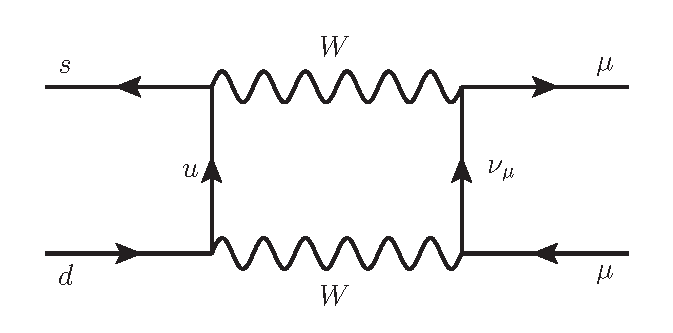
\includegraphics[width=\linewidth]{figs/theory/KToMuMu_uquark.eps}
\caption{}
\label{fig:ktomm:a}
\end{subfigure}
\begin{subfigure}{0.49\textwidth}
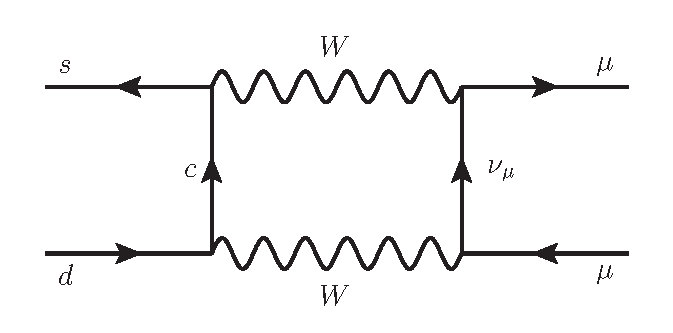
\includegraphics[width=\linewidth]{figs/theory/KToMuMu_cquark.eps}
\caption{}
\label{fig:ktomm:b}
\end{subfigure}
\caption{Feynman diagrams contributing to the decay \decay{\Kz}{\mumu}. The amplitude for each diagram is proportional to the product of the coupling at each vertex: (a) $\sin\theta_{C}\cos\theta_{C}$, (b)  $-\sin\theta_{C}\cos\theta_{C}$. The total amplitude is found by summing the two contributions.}
\label{fig:ktomm}
\end{figure}

In the Cabibbo-GIM scheme, it can be intepreted that the \W does not couple to the mass eigenstates \dquark and \squark but instead to the weak eigenstates $\dquark^\prime$ and $\squark^\prime$, given by

\begin{equation}
\dquark^\prime = \dquark\cos\theta_{C}+\squark\sin\theta_{C},~~~\squark^\prime = -\dquark\sin\theta_{C}+\squark\cos\theta_{C}
\end{equation}

\noindent or in `Cabibbo matrix' form

\begin{equation}
\binom{\dquark^\prime}{\squark^\prime} = 
\begin{pmatrix}
\cos\theta_{C} & \sin\theta_{C} \\
-\sin\theta_{C} & \cos\theta_{C} \\
\end{pmatrix}
\binom{\dquark}{\squark}.
\end{equation}

Even before the discovery of the \cquark quark, Kobayaski and Maskawa~\cite{kobayashi-maskawa} had generalised the Cabibbo-GIM scheme to incorporate three generations of quarks. This was motivated by the desire to explain \CP violation within the Cabibbo-GIM scheme, which was not possible with only two generations. The weak eigenstates are related to the mass eigenstates through the CKM matrix

\begin{equation}
\begin{pmatrix}
\dquark^\prime \\
\squark^\prime \\
\bquark^\prime \\
\end{pmatrix}
=
\begin{pmatrix}
\Vud & \Vus & \Vub \\
\Vcd & \Vcs & \Vcb \\
\Vtd & \Vts & \Vtb \\
\end{pmatrix}
\begin{pmatrix}
\dquark \\
\squark \\
\bquark \\
\end{pmatrix}
\end{equation}

\noindent where each matrix element, \Vij, specifies the coupling of $i$ to $j$. The additional generation of quarks increases the number of free parameters from one ($\theta_{C}$) to four: three `generalised Cabibbo angles' ($\theta_{12}$, $\theta_{23}$, $\theta_{13}$) and a complex phase $\delta$. This complex phase generates \CP violation in the quark sector. 

\subsection{Beyond the SM}
\label{sec:theory:limitations}

Despite its considerable success in predicting cross-sections and branching ratios of particles with great accuracy, the SM is not without its limitations, some of which are outlined below

\begin{itemize}
  \item Gravity, the fourth fundamental force, is not incorporated in the SM. However, this is not specific to the SM as there is no consensus on how to include gravity in a QFT. 
  \item The SM has 19 free parameters: the 9 fermion masses, the 4 parameters of the CKM matrix, 3 gauge coupling constants, the Higgs vacuum expectation value $v$, the Higgs quartic coupling $\lambda$ and the QCD $\theta$ parameter. 
  \item Dark matter, which is believed to be five times as abundant as ordinary matter, is not accounted for in the SM.
  \item The amount of \CP violation predicted by the SM is ten orders of magnitude lower than what is needed to account for the observed matter-antimatter asymmetry in the Universe, assuming matter and antimatter were created in equal amounts in the Big Bang.
  \item The measured mass of the Higgs boson implies a large cancellation between the bare mass and quantum corrections. The nature of a mechanism that could provide a natural cancellation of these corrections is unknown.
\end{itemize}

\noindent These limitations have led physicists to look for extensions to the SM in the form of New Physics (NP) models. Such NP models often predict new particles that may contribute to, and therefore modify, flavour-changing processes in the SM.

\subsection{Rare decays of \B mesons}
\label{sec:theory:rare}

Flavour-changing neutral current (FCNC) transitions are forbidden at tree level in the SM. They are rare processes that occur via loop and box diagrams, making them an ideal place to perform a search for NP. Rare decays of \B mesons, such as those containing a \btosll transition, can have sizeable NP contributions that are not swamped by the competing SM process. 

By studying the properties of FCNC processes it is possible to perform model independent searches sensitive to a wide range of NP models. Feyman diagrams for the \btosll transition, both in the SM and in possible NP scenarios~\cite{Gauld:2013qja,Altmannshofer:2014cfa,Crivellin:2015mga}, are shown Fig.~\ref{fig:btosll}. New particles can modify the dynamics of a decay: changing the branching fraction or the kinematic distribution of the final state particles. By comparing the SM prediction of observables with experimental measurements, the flavour structure of NP models can be probed. The theoretical framework used to interpret flavour physics measurements in a model independent way is the so-called Operator Product Expansion (OPE)~\cite{ope}.

\begin{figure}[!tb]
\centering
\begin{subfigure}{0.49\textwidth}
\begin{tikzpicture}
\node[anchor=south west,inner sep=0](image) at (0,0) {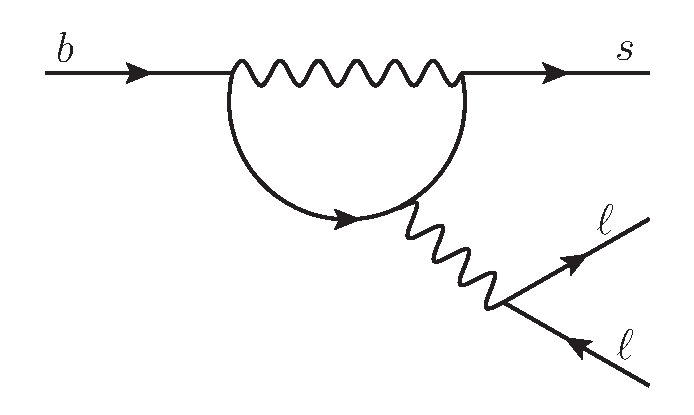
\includegraphics[width=\textwidth]{figs/theory/btosll_penguin.eps}};
\begin{scope}[x={(image.south east)},y={(image.north west)}]
%\draw[help lines,xstep=.1,ystep=.1] (0,0) grid (1,1);
\node[draw=none,bleudefrance] at (0.53,0.96) {\small \Wm};
\node[draw=none,bleudefrance] at (0.3,0.6) {\small \tquark};
\node[draw=none,bleudefrance] at (0.56,0.27) {\small \Pgamma, $\Z^{0}$};
\node[draw=none,bleudefrance] at (0.2,0.2) {SM};
\end{scope}
\end{tikzpicture}
\caption{}
\label{fig:btosll:a}
\end{subfigure}
\begin{subfigure}{0.49\textwidth}
\begin{tikzpicture}
\node[anchor=south west,inner sep=0](image) at (0,0) {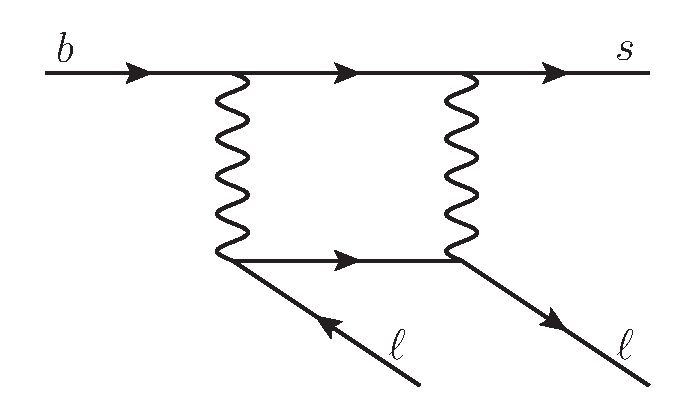
\includegraphics[width=\textwidth]{figs/theory/btosll_box.eps}};
\begin{scope}[x={(image.south east)},y={(image.north west)}]
%\draw[help lines,xstep=.1,ystep=.1] (0,0) grid (1,1);
\node[draw=none,bleudefrance] at (0.5,0.95) {\small \tquark};
\node[draw=none,bleudefrance] at (0.25,0.6) {\small \Wm};
\node[draw=none,bleudefrance] at (0.8,0.6) {\small \Wp};
\node[draw=none,bleudefrance] at (0.5,0.45) {\small \Pnu};
\node[draw=none,bleudefrance] at (0.2,0.2) {SM};
\end{scope}
\end{tikzpicture}
\caption{}
\label{fig:btosll:b}
\end{subfigure}
\begin{subfigure}{0.49\textwidth}
\begin{tikzpicture}
\node[anchor=south west,inner sep=0](image) at (0,0) {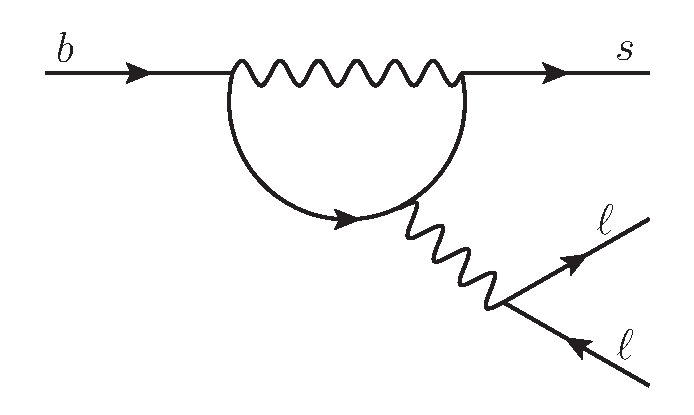
\includegraphics[width=\textwidth]{figs/theory/btosll_penguin.eps}};
\begin{scope}[x={(image.south east)},y={(image.north west)}]
%\draw[help lines,xstep=.1,ystep=.1] (0,0) grid (1,1);
\node[draw=none,bostonuniversityred] at (0.5,0.96) {\small $\tilde{g}$};
\node[draw=none,bostonuniversityred] at (0.3,0.6) {\small $\tilde{d}_{i}$};
\node[draw=none,bostonuniversityred] at (0.58,0.27) {\small $\H$};
\node[draw=none,bostonuniversityred] at (0.2,0.2) {NP};
\end{scope}
\end{tikzpicture}
\caption{}
\label{fig:btosll:c}
\end{subfigure}
\begin{subfigure}{0.49\textwidth}
\begin{tikzpicture}
\node[anchor=south west,inner sep=0](image) at (0,0) {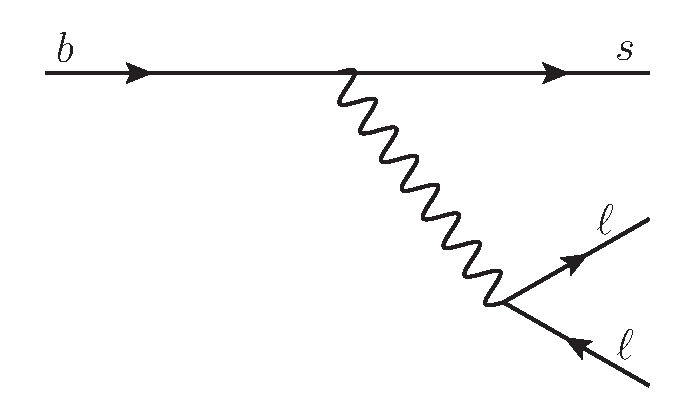
\includegraphics[width=\textwidth]{figs/theory/btosll_zprime.eps}};
\begin{scope}[x={(image.south east)},y={(image.north west)}]
%\draw[help lines,xstep=.1,ystep=.1] (0,0) grid (1,1);
\node[draw=none,bostonuniversityred] at (0.55,0.45) {\small $Z^{'}$};
\node[draw=none,bostonuniversityred] at (0.2,0.2) {NP};
\end{scope}
\end{tikzpicture}
\caption{}
\label{fig:btosll:d}
\end{subfigure}
\caption{Feynman diagrams for the FCNC transition \btosll: in the SM (a,b) and in possible NP scenarios (c,d).}
\label{fig:btosll}
\end{figure}

In the OPE approach, all degrees of freedom above a given energy scale, $\Lambda$, are integrated out. This is valid as long as $\Lambda$ is much larger than the energy scale of the decay, $\mu$, which for the study of \B mesons is chosen to be $\order(m_{\bquark})$. This formalism is analogous to Fermi's effective theory of weak decay in which the full theory is reduced to a four point interaction, as shown in Fig.~\ref{fig:beta} for $\beta$-decay.

\begin{figure}[!tb]
\centering
\begin{subfigure}{0.49\textwidth}
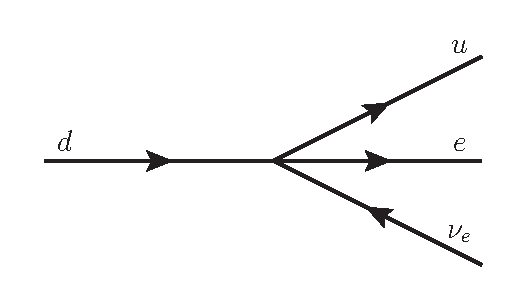
\includegraphics[width=\linewidth]{figs/theory/beta_4point.eps}
\caption{}
\label{fig:beta:a}
\end{subfigure}
\begin{subfigure}{0.49\textwidth}
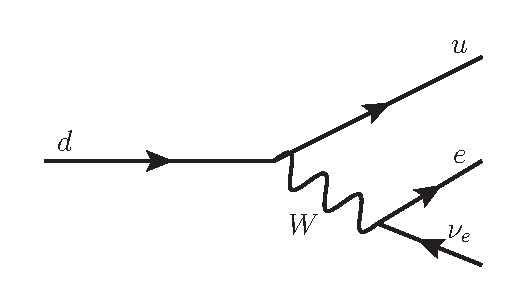
\includegraphics[width=\linewidth]{figs/theory/beta_w.eps}
\caption{} 
\label{fig:beta:b}
\end{subfigure}
\caption{Feynman diagrams for $\beta$-decay in the (a) effective theory and (b) full theory.}
\label{fig:beta}
\end{figure}

In the SM, the effective Hamiltonian describing \btosll decays can be written as

\begin{equation}
\mathcal{H}_{\rm eff} = - \frac{4G_{F}}{\sqrt{2}}V_{tb}V^{*}_{ts}\sum_{i}[\mathcal{C}_{i}(\mu)\mathcal{O}_{i}(\mu) + \mathcal{C}^{'}_{i}(\mu)\mathcal{O}^{'}_{i}(\mu)].
\end{equation}

\noindent where $G_{F}$ is the Fermi constant and $V_{ij}$ are CKM matrix elements. The complex Wilson coefficients, $\mathcal{C}_{i}$, incorporate the short distance (high energy) contributions. For each Wilson coefficient, there is a local operator $\mathcal{O}_{i}$ which incorporates the long distance (low energy) contributions. The primed operators represent the right-handed currents, which are highly suppressed in the SM. The advantage of the OPE approach is that the Wilson coefficients are independent of the underlying process and can include contributions from NP. 

For \btosll decays, the dominant contributions in the SM arise from the following operators~\cite{operators}

\begin{alignat}{2}
&\order_{7} = \frac{e}{g^{2}}m_{\bquark}(\squarkbar\sigma_{\mu\nu}P_{R}\bquark)F^{\mu\nu},~~~~~&&\order_{7}^{\prime} = \frac{e}{g^{2}}m_{\bquark}(\squarkbar\sigma_{\mu\nu}P_{L}\bquark)F^{\mu\nu}, \nonumber \\
&\order_{9} = \frac{e^{2}}{g^{2}}(\squarkbar\gamma_{\mu}P_{L}\bquark)(\ellbar\gamma^{\mu}\ell), &&\order_{9}^{\prime} = \frac{e^{2}}{g^{2}}(\squarkbar\gamma_{\mu}P_{R}\bquark)(\ellbar\gamma^{\mu}\ell), \nonumber \\
&\order_{10} = \frac{e^{2}}{g^{2}}(\squarkbar\gamma_{\mu}P_{L}\bquark)(\ellbar\gamma^{\mu}\gamma_{5}\ell), &&\order_{10}^{\prime} = \frac{e^{2}}{g^{2}}(\squarkbar\gamma_{\mu}P_{R}\bquark)(\ellbar\gamma^{\mu}\gamma_{5}\ell), \\
&\order_{S} = \frac{e^{2}}{16\pi^{2}}m_{\bquark}(\squarkbar P_{R}\bquark)(\ellbar\ell), &&\order_{S}^{\prime} = \frac{e^{2}}{16\pi^{2}}m_{\bquark}(\squarkbar P_{L}\bquark)(\ellbar\ell), \nonumber\\
&\order_{P} = \frac{e^{2}}{16\pi^{2}}m_{\bquark}(\squarkbar P_{R}\bquark)(\ellbar\gamma_{5}\ell), &&\order_{P}^{\prime} = \frac{e^{2}}{16\pi^{2}}m_{\bquark}(\squarkbar P_{L}\bquark)(\ellbar\gamma_{5}\ell), \nonumber
\end{alignat}

\noindent where $P_{L/R} = (1\mp\gamma_{5})/2$ are the left- and right-handed projection operators. The operator $\order_{7}$ is the electromagnetic operator corresponding to the emission of a photon. The vector and axial-vector operators, $\order_{9}$ and $\order_{10}$, describe the $Z$ penguin and $W$ box diagrams. The operators $\order_{S}$ and $\order_{P}$ represent scalar and pseudoscalar operators.


\clearpage
\section{The \lhcb experiment}
\label{sec:lhcb}

% This chapter provides a detailed description of the experimental complex and apparatus relevant to this thesis. It begins with a brief description of \cern and the \lhc, followed by a detailed overview of the \lhcb experiment, both present and future.

\subsection{\lhc}
\label{sec:lhcb:lhc}

The Large Hadron Collider (\lhc) at the European Organization for Nuclear Research (\cern) is a particle accelerator designed to collide protons at a center-of-mass energy (\sqs) of 14\tev~\cite{lhc}. It has a peak design (instantaneous) luminosity of \lum$= 10^{34}\cm^{-2}\sec^{-1}$ for proton operation. It is also used to accelerate heavy ions. The accelerator complex at \cern is shown in Fig.~\ref{fig:lhc}. The four main experiments on the \lhc are \atlas, \cms, \lhcb and \alice. \atlas and \cms are both multipurpose experiments, while \alice is used for the study of heavy ion collisions. The present thesis concerns the \lhcb experiment, of which an overview of the goals and design of the experiment is given below.

\begin{figure}[!b]
\centering
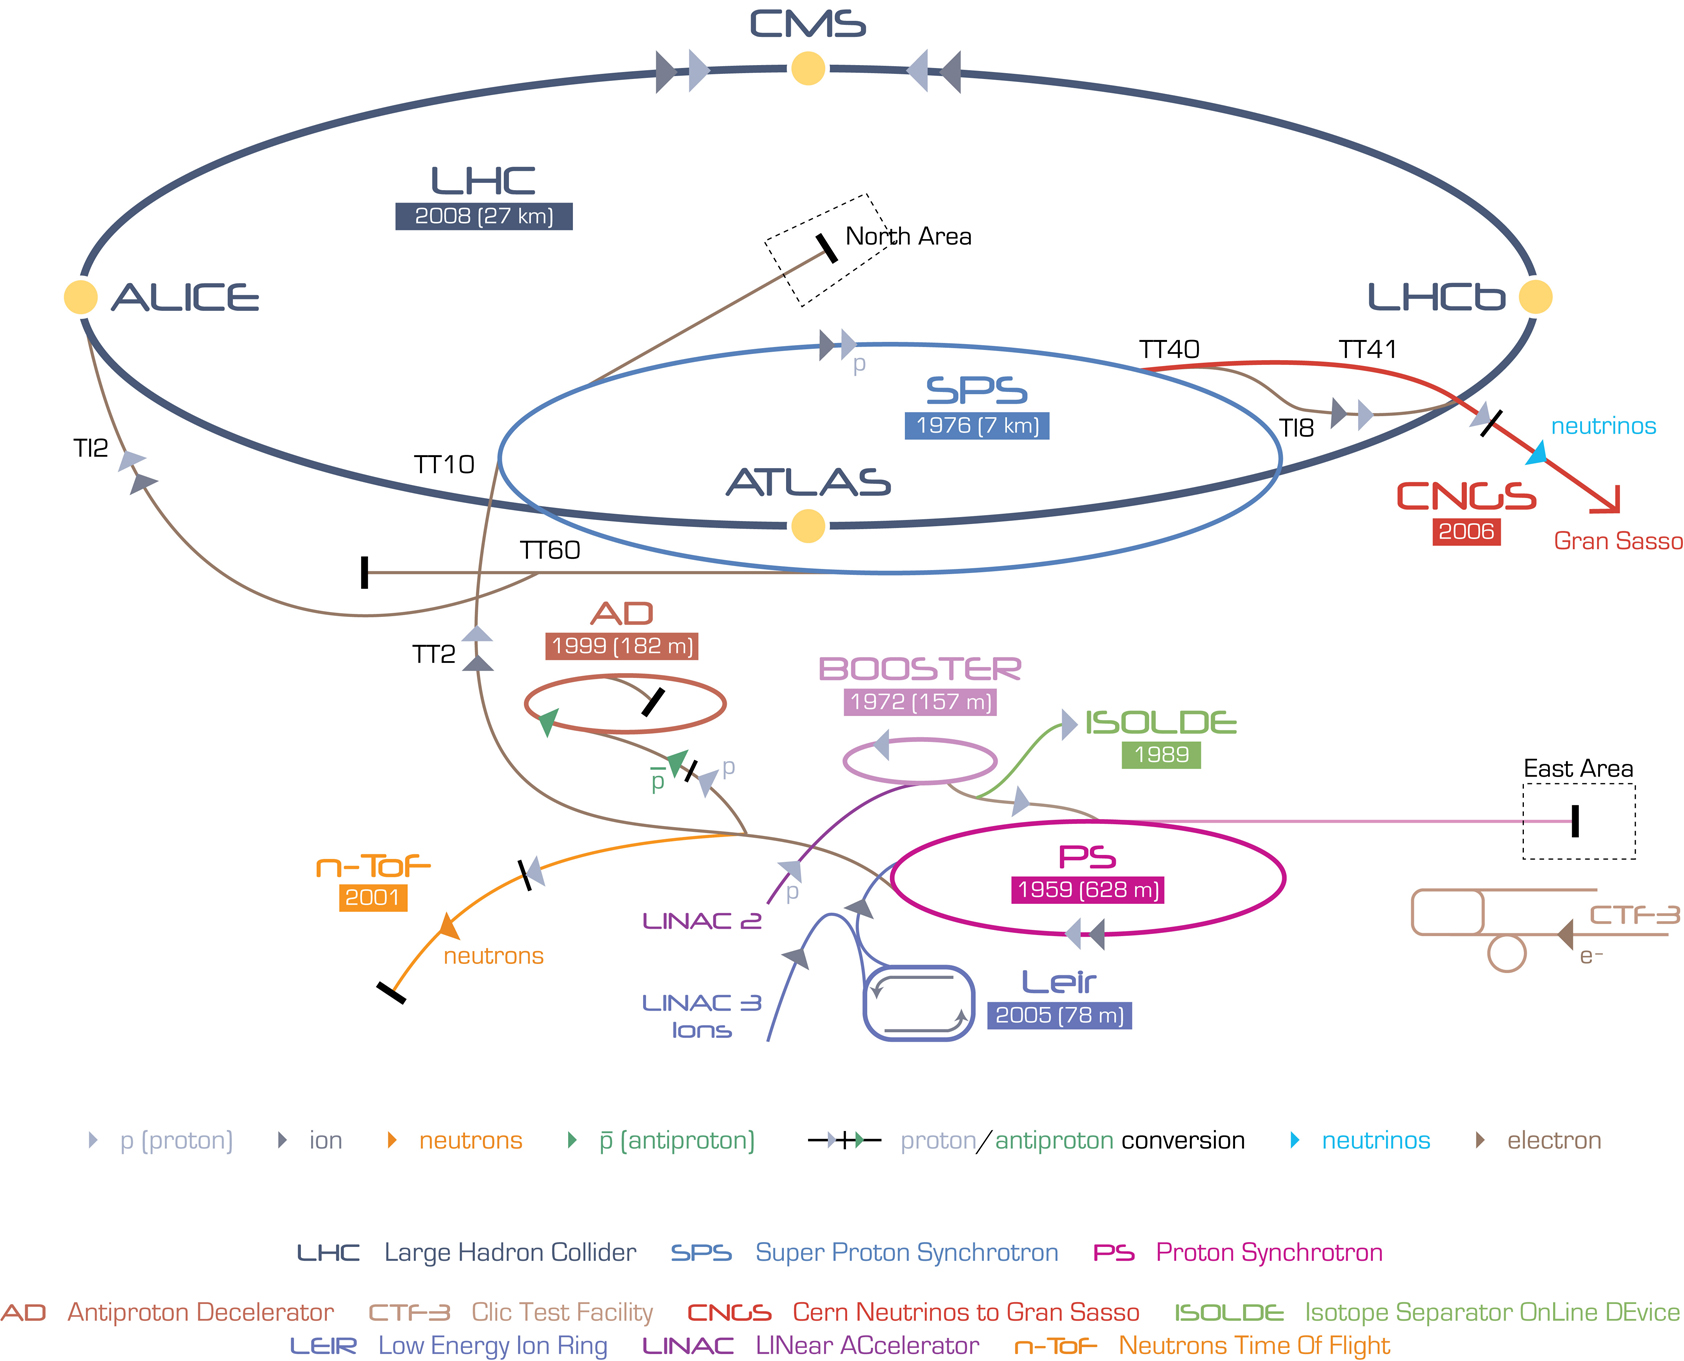
\includegraphics[width=\textwidth]{figs/detector/lhc.jpg}
\caption{Schematic view of the CERN accelerator complex.}
\label{fig:lhc}
\end{figure}

\subsection{\lhcb experiment}
\label{sec:lhcb:lhcb}

\lhcb is a dedicated heavy flavour experiment with the primary goal of searching for indirect evidence of NP in \CP violation and rare decays of beauty and charm hadrons~\cite{lhcb}. During Run 1 of the \lhc (2010-2013), the \lhcb experiment took data at center-of-mass energies of \sqs = 7-8\tev. Due to the large beauty and charm production cross-sections provided by the \lhc, the \lhcb experiment was able to collect $\sim$10$^{12}$ heavy flavour decays during data taking in 2011 and 2012~\cite{LHCb-DP-2014-002}.

The data used for physics analysis in Chapter~\ref{sec:kpimm} was collected in 2011 and 2012. In 2011, the center-of-mass energy was 7\tev and the majority of the data was taken at a instantaneous luminosity of $3.5\times10^{32}\cm^{-2}\sec^{-1}$. In 2012, the center-of-mass energy was increased to 8\tev and the data was taken at a instantaneous luminosity of $4\times10^{32}\cm^{-2}\sec^{-1}$. This corresponds to an integrated luminosity of 1\invfb in 2011 and 2\invfb in 2012.

The \lhcb detector is a single arm forward spectrometer that covers a pseudo-rapidity range of $2 < \eta < 5$. The layout of the \lhcb detector, shown schematically in Fig.~\ref{fig:lhcb-run1}, is motivated by the physics of \bquark quark production at the \lhc. The leading order production processes for \bquark\bquarkbar pairs in \proton\proton collisions are gluon-gluon fusion and quark-antiquark annihilation, as illustrated in Fig.~\ref{fig:b-production}. In the high energy collisions present at the \lhc, the \bquark\bquarkbar pairs tend to be produced in the same forward or backward cone, shown in Fig.~\ref{fig:b_bbar_correlation}.  Therefore, due to its unique geometry, \lhcb is able to detect $\sim40\%$ of the heavy quark pairs despite covering only $\sim4\%$ of the total solid angle.

The following requirements are crucial in order to fulfil the \lhcb physics programme: efficient, robust and flexible triggering on a variety of different final states, excellent tracking (momentum, impact parameter (IP) and primary vertex (PV) resolution), precise decay time resolution and excellent particle identification. The importance of each of these requirements are discussed in detail in the following sections.

\begin{sidewaysfigure}
\centering
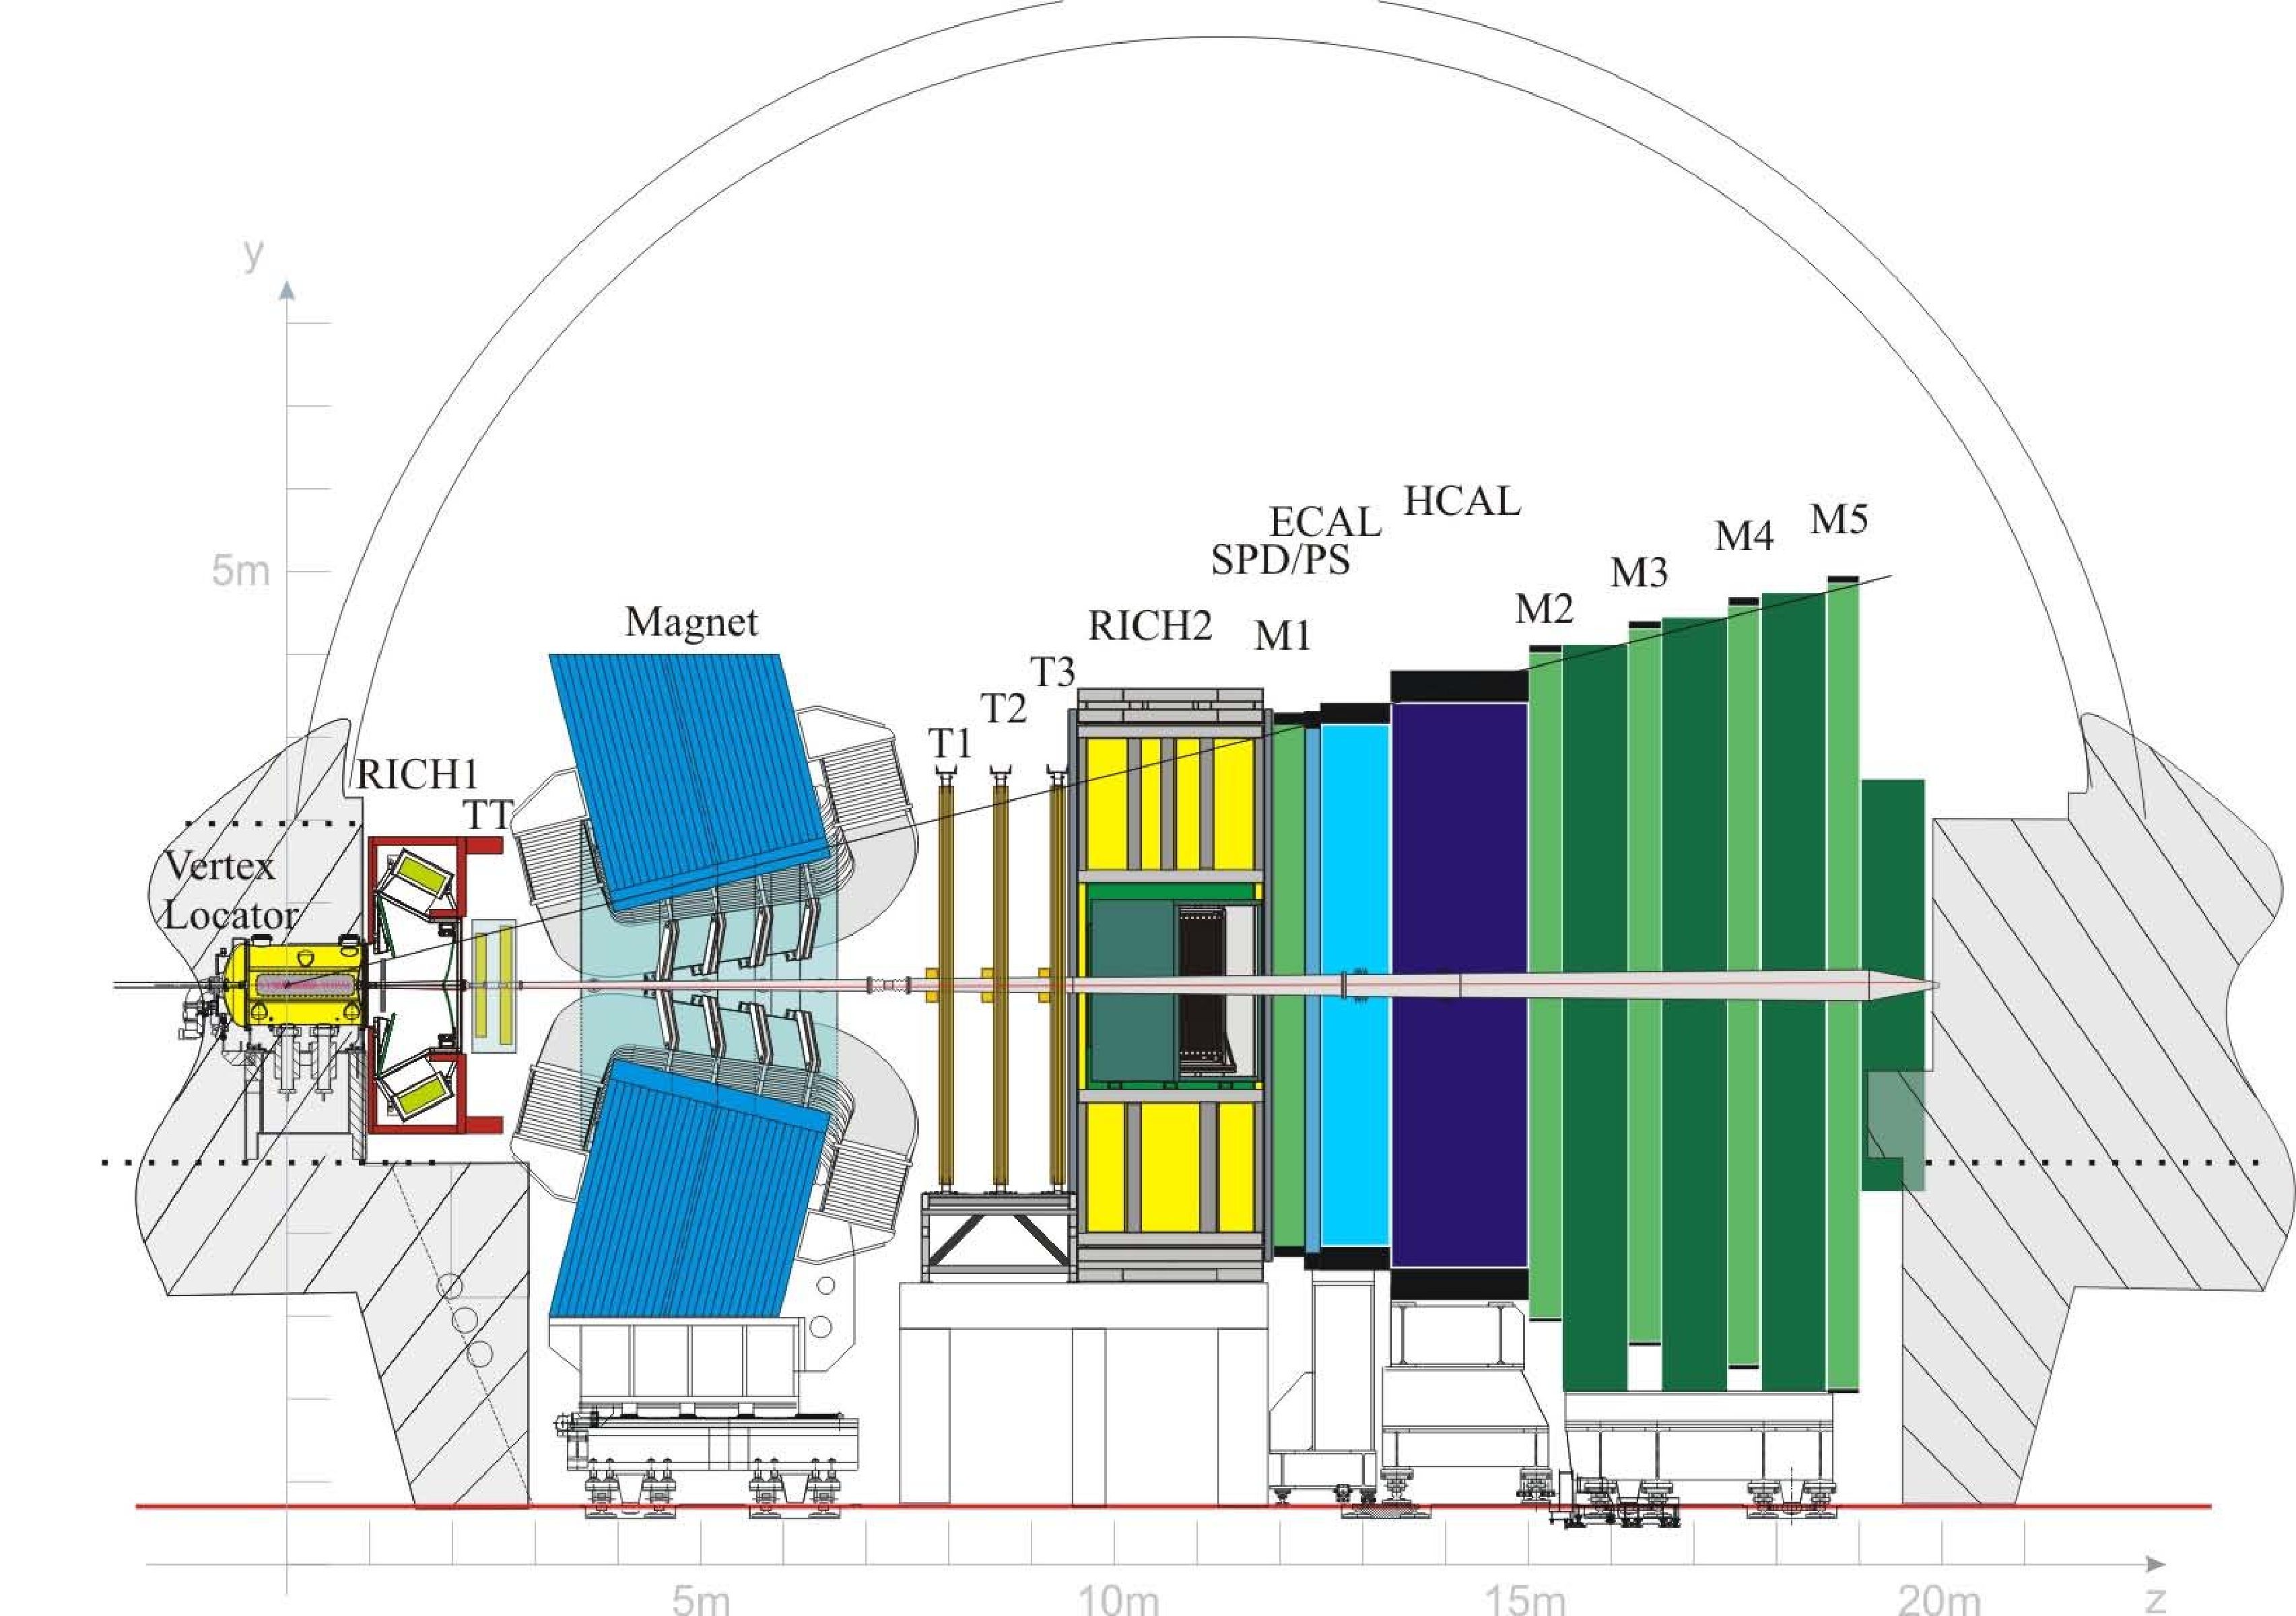
\includegraphics[width=0.9\textwidth]{figs/detector/lhcb-run1.pdf}
\caption{Schematic view of the \lhcb detector.}
\label{fig:lhcb-run1}
\end{sidewaysfigure}

\begin{figure}[!tb]
\centering
\begin{subfigure}{0.4\textwidth}
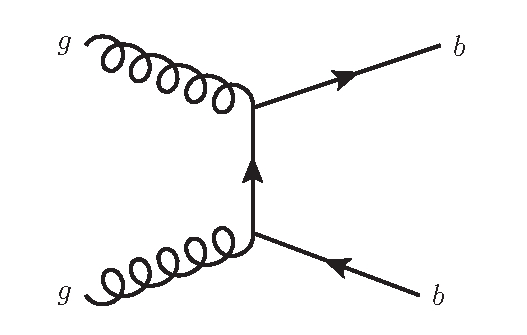
\includegraphics[width=\linewidth]{figs/detector/gluon_fusion.eps}
\caption{}
\label{fig:b-production:a}
\end{subfigure}
\begin{subfigure}{0.4\textwidth}
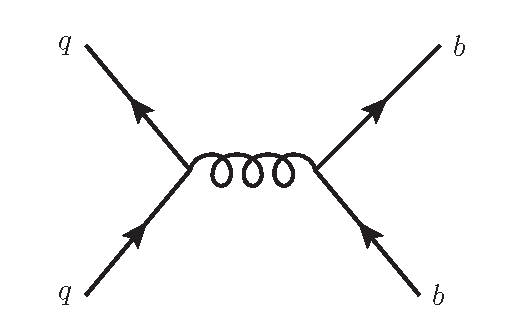
\includegraphics[width=\linewidth]{figs/detector/quark_antiquark_annihilation.eps}
\caption{}
\label{fig:b-production:b}
\end{subfigure}
\caption{Feynman diagrams of the leading order production processes for \bquark\bquarkbar pairs in proton-proton collisions. These are (a) gluon-gluon fusion and (b) quark-antiquark annihilation~\cite{b-production}.}
\label{fig:b-production}
\end{figure}

\begin{figure}[!tb]
\centering
\includegraphics[width=0.5\textwidth]{figs/detector/b_bbar_correlation.pdf}
\caption{The angular distribution of \bquark\bquarkbar pairs in terms of the polar angle from the beam axis. The red area shows the acceptance of the \lhcb detector.}
\label{fig:b_bbar_correlation}
\end{figure}


\subsubsection{Dipole magnet}

A warm dipole magnet~\cite{LHCb-TDR-001} is used in order to allow a measurement of the momentum of charged particles in the forward acceptance of $\pm$250\mrad vertically and $\pm$300\mrad horizontally. It provides an integrated magnetic field of 4~Tm for tracks of 10\m in length. The $\hat{y}$-component of the magnetic field, $B_{y}$, as a function of $z$ is shown in Fig.~\ref{fig:magnet}. The location of the tracking sub-detectors, described in Sec.~\ref{sec:lhcb:tracking}, are also shown. The polarity of the magnetic field is changed regularly in order to be able to control possible detection asymmetries.

\begin{figure}[!tb]
\centering
\adjincludegraphics[width=\textwidth,trim={{.1\width} {.62\height} {.1\width} {.1\height}},clip]{figs/detector/magnet.pdf}
\caption{The strength of the main component of the magnetic field, $B_{y}$, as a function of $z$. The location of the tracking sub-detectors are shown.}
\label{fig:magnet}
\end{figure}

\subsubsection{Tracking system}
\label{sec:lhcb:tracking}

The trajectories of charged particles traversing the \lhcb detector are reconstructed using a dedicated tracking system. The tracking system consists of a high granularity vertex detector surrounding the \proton\proton interaction region, a large area silicon-strip detector located upstream of the magnet, and three stations of silicon-strip detectors and straw drift tubes placed downstream of the magnet. By determining the deflection of the charged particles that have passed through the magnetic field their momentum can be measured.

The Vertex Locator (\velo)~\cite{LHCb-TDR-005,LHCb-DP-2014-001} is a silicon microstrip detector that provides measurements of track coordinates close to the \proton\proton interaction region. These precision measurements are used to identify both the primary interaction vertices and the displaced secondary vertices of the decays of \bquark and \cquark hadrons. The detector consists of 42 silicon micro-strip stations with $r$-$\phi$ geometry, shown schematically in Fig.~\ref{fig:velo}. It has two retractable halves which are opened and closed during each \lhc fill. When closed, the sensors are positioned only 7\mm from the \lhc beam. This is essential in achieving precise IP measurements.

\begin{figure}[!tb]
\centering
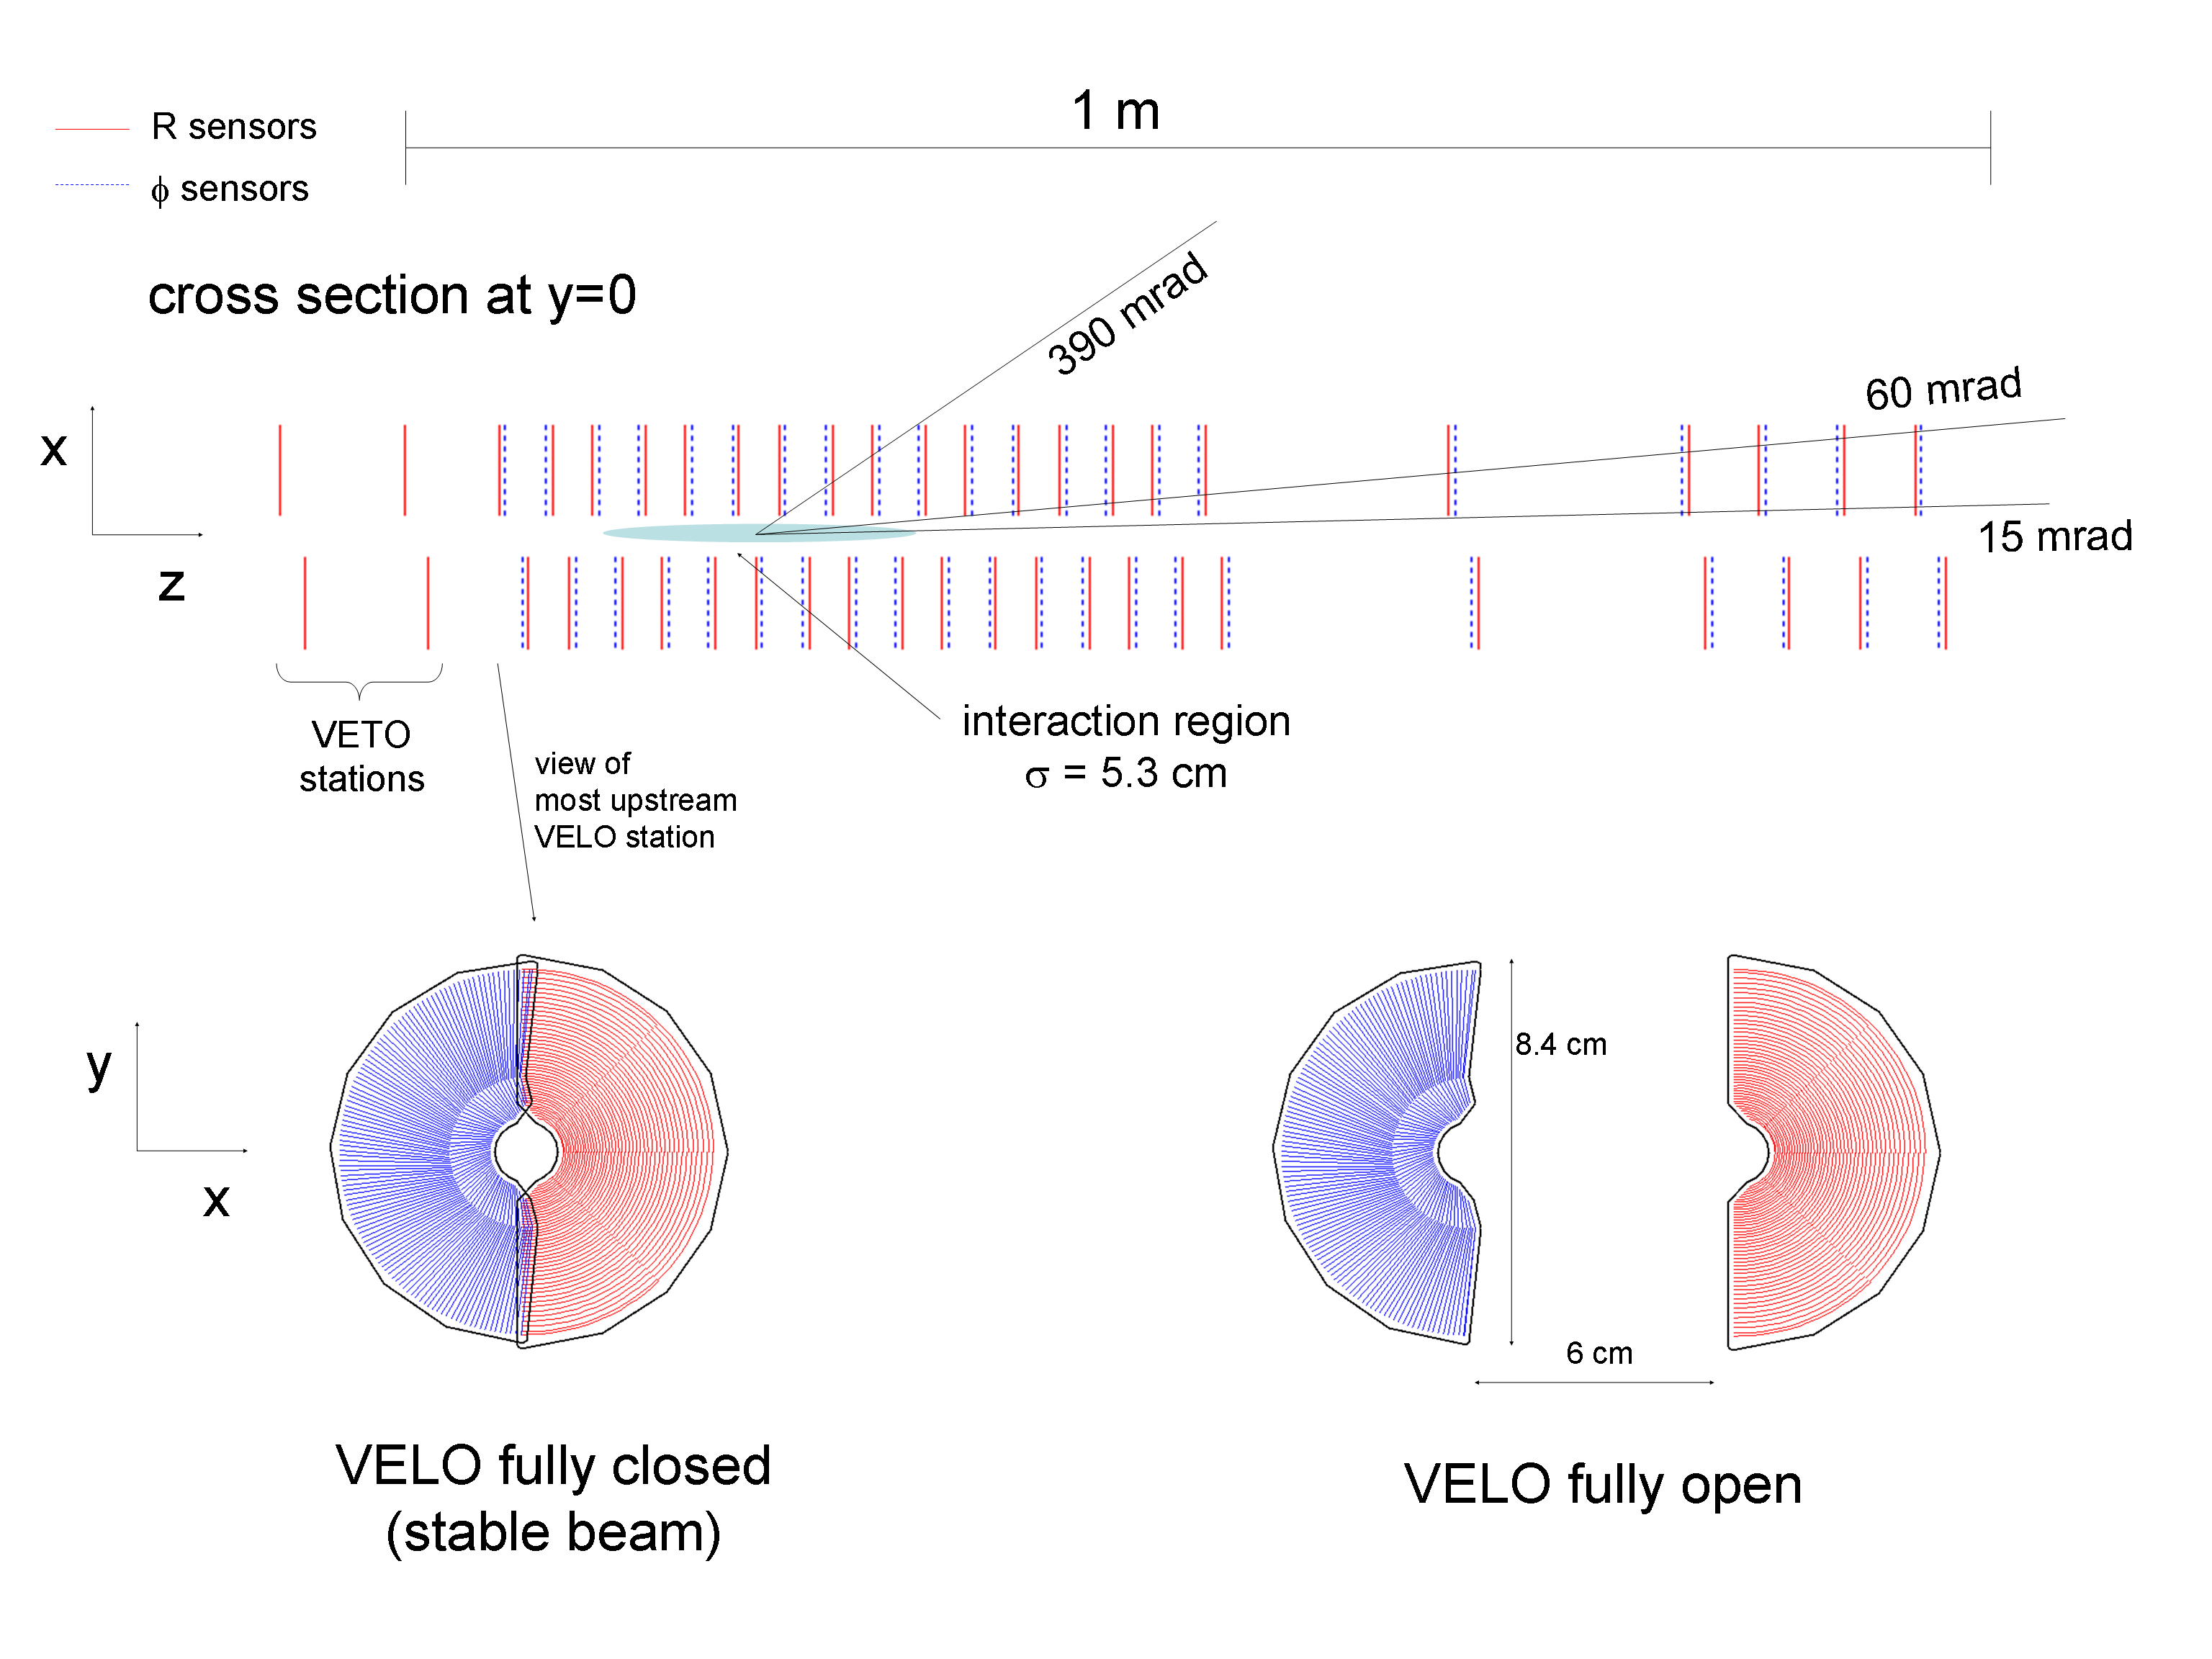
\includegraphics[width=\textwidth]{figs/detector/velo.png}
\caption{Schematic view of the \velo detector.}
\label{fig:velo}
\end{figure}

The Silicon Tracker (ST) consists of two silicon microstrip detectors: the Tracker Turicensis\footnote{Formerly known as the Trigger Tracker.} (TT)~\cite{LHCb-TDR-009} and the Inner Tracker (IT)~\cite{LHCb-TDR-008}. The TT is located upstream of the magnet and covers the full acceptance of the experiment. The IT is located downstream of the magnet and covers a cross-shaped region at the center of the three tracking stations. Each ST station contains four layers with a \mbox{$x$-$u$-$v$-$x$} layout such that the $u$ and $v$ layers are tilted by $\pm$ 5$^{\circ}$ with respect to the vertical. The inclined layers allow stereo measurements to be made. A schematic view of the TT sub-detector is shown in Fig.~\ref{fig:tt}. As the beampipe passes through the TT there is a square hole at the center of the detector which reduces its acceptance. The square hole has a width of 7.7\cm at the first TT sub-station (TTa) and 8.0\cm at the second (TTb).

\begin{figure}[!tb]
\centering
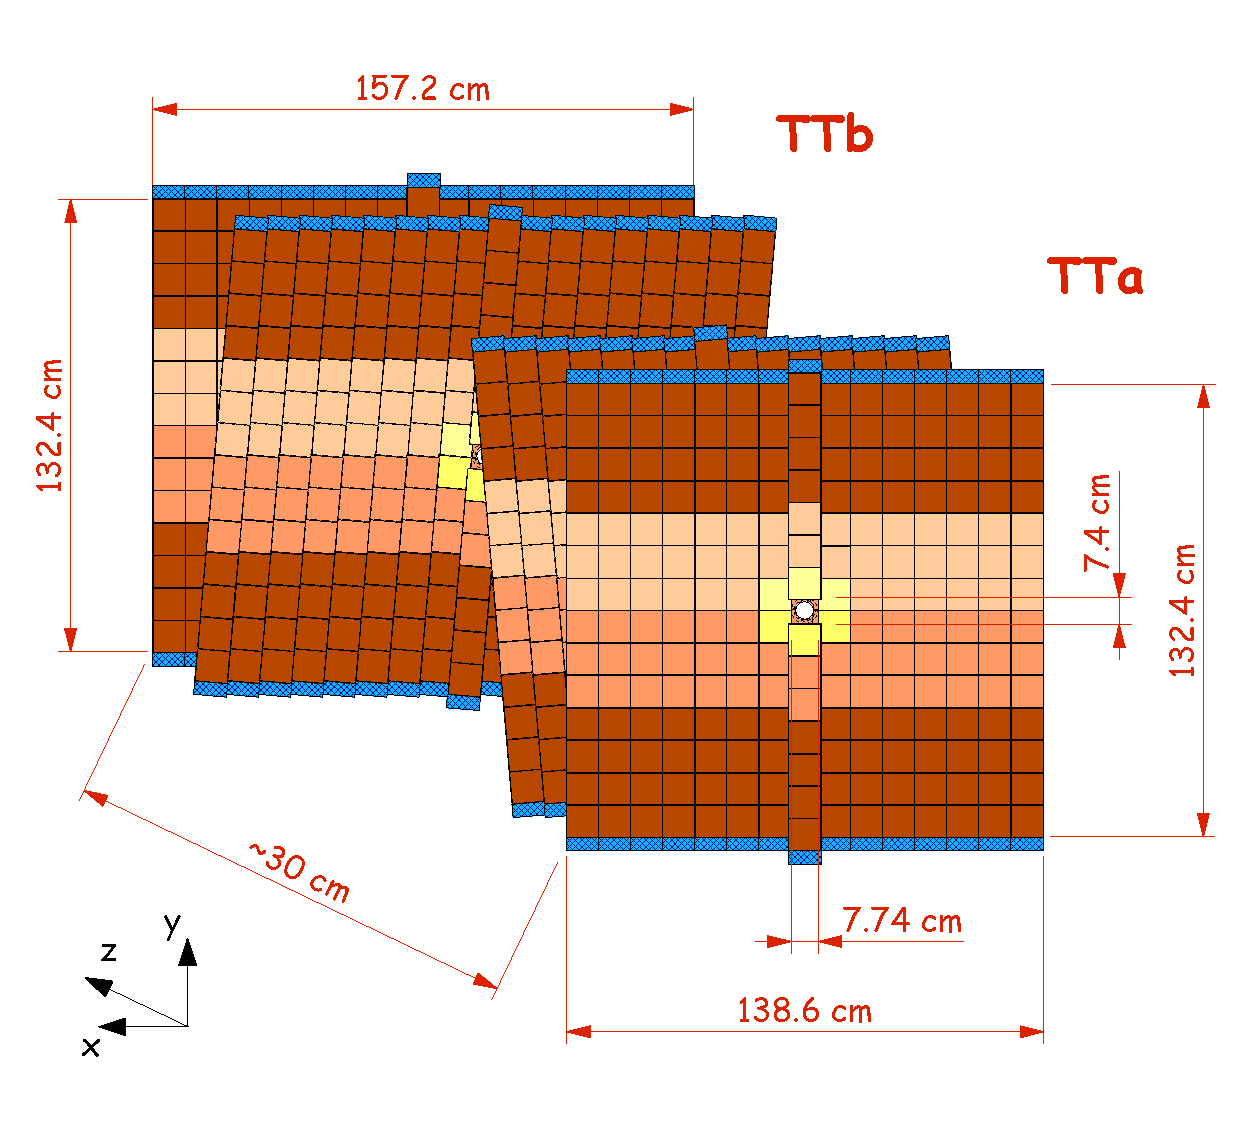
\includegraphics[width=0.8\textwidth]{figs/detector/tt.pdf}
\caption{Schematic view of the TT sub-detector geometry. The different colours indicate the number of sensors that are wire bonded together in the $y$ direction.}
\label{fig:tt}
\end{figure}

The Outer Tracker (OT)~\cite{LHCb-TDR-006,LHCb-DP-2013-003,LHCb-DP-2014-002} is a drift-time detector made up of arrays of individual straw-tube modules. The modules each contain two staggered layers of drift-tubes of 4.9\mm in diameter. They are filled with a mixture of Argon (70\%), \cotwo (28.5\%) and $\mathrm{O}_{2}$ (1.5\%), which provides both fast drift times and sufficient drift-coordinate resolution. The detector consists of three stations each with four layers arranged with a \mbox{$x$-$u$-$v$-$x$} layout such that the $u$ and $v$ layers are tilted by $\pm$ 5$^{\circ}$ with respect to the vertical.

The track reconstruction efficiency can be defined as the probability that the trajectory of a charged particle that has passed through the full tracking system is reconstructed. This can be measured in data using a tag-and-probe method with \decay{\jpsi}{\mumu} decays~\cite{LHCb-DP-2013-002}. One of the daughters is fully reconstructed (tag), while the other is only partially (probe), although well enough to reconstruct the $J/\psi$ invariant mass.  The efficiency can then be measured by matching the probe track to a fully reconstructed track. The average efficiency is found to be over 95\% and is only slightly affected in high multiplicity events~\cite{LHCb-DP-2013-002}.

The momentum resolution for tracks passing through the full tracking system can be measured in data using \decay{\jpsi}{\mumu} decays. The relative momentum resolution, $\delta p/p$, is found to be between 0.4\% - 0.6\% for tracks up to 100\gevc~\cite{LHCb-DP-2014-002}. The mass resolution is determined from data by studying the \jpsi, \psitwos, $\Upsilon$ and \Z resonances. The relative mass resolution, $\sigma_{m}/m$, is found to be about 5 per mille up to the $\Upsilon$ masses~\cite{LHCb-DP-2014-002}.

Precise vertex resolution is important to allow the separation of primary and secondary decay vertices. The primary vertex resolution depends strongly on the number of tracks used to form it. It can be measured in data in an event-by-event manner by randomly splitting the track sample in two and reconstructing the PV using each independent set of tracks. In 2011 data, a 25-track vertex was found to have a resolution of 13\mum in $x$ and $y$ and 71\mum in $z$~\cite{LHCb-DP-2014-002}.
 
While the reconstructed decay time of charm and beauty hadrons is used in offline selections and for precise measurements of lifetimes, the most stringent requirement on the decay time resolution originates from the need to resolve the fast \Bs-\Bsb oscillations in mixing. The decay time resolution is topology dependent and is calibrated in data for each final state using prompt combinations that fake the signal candidates. The shape of the prompt decay time distribution is determined only by the resolution function. The typical decay time resolution is 45\fs for a 4-track vertex~\cite{LHCb-DP-2014-002}.

\subsubsection{Particle identification}
\label{sec:lhcb:pid}

Excellent particle identification (PID) is a crucial requirement for \lhcb. Charged particle identfication is important to be able to distinguish specific final states from those with otherwise identical topologies and to perform \bquark quark flavour tagging. Detecting photons is essential to allow the reconstruction of rare radiative decays. As muons are present in the final state of many \CP-sensitive decays, such as \BsToJPsiPhi, and rare decays, such as \BsToMuMu, their triggering and identification are of fundamental importance.

The \lhcb detector has several specific systems in order to perform the various particle identification tasks. The primary goal of the \rich system~\cite{LHCb-TDR-009,LHCb-DP-2012-003} is the identification of charged hadrons (\pion, \kaon, \proton). This is achieved by exploiting the Cherenkov effect by which a charged particle travelling in a medium will emit Cherenkov radiation whenever the velocity of the particle exceeds the velocity of light in that medium. The cone of light will be emitted at a particular angle ($\theta_{c}$) relative to the particle path. \rich detectors use a combination of spherical and flat mirrors to focus the cone of light into a ring. This ring is then projected onto an array of photodetectors. The Cherenkov angle ($\theta_{c}$) can be determined from the radius of the ring. The velocity of the particle is found from $\theta_{c}$.\footnote{$\cos\theta_{c} = \frac{1}{n\beta}$ where $\beta = \frac{v}{c}$ and $n$ is the refractive index of the medium.} Combining this velocity with the momentum measured by the tracking systems allows the determination of the particle mass and, therefore, the type of particle. 

In the forward region covered by the \lhcb experiment, there is a strong anticorrelation between polar angle and momentum. Due to this, the \rich system consists of two detectors. The detector upstream of the magnet, \richone, covers the low and intermediate momentum region 2-40\gevc for the full angular acceptance 15-300\mrad. The downstream detector, \richtwo, covers the high momentum region 15-100\gevc over a reduced angular acceptance 15-120\mrad. During Run 1, \richone contained aerogel and \cfourften as gas radiators while \richtwo contained \cffour.\footnote{The aerogel was removed during Long Shutdown 1 (2013-2015).} The relationship between Cherekov angle and particle momentum is shown in Fig.~\ref{fig:radiators} for each of the three radiators.

\begin{figure}[!tb]
\centering
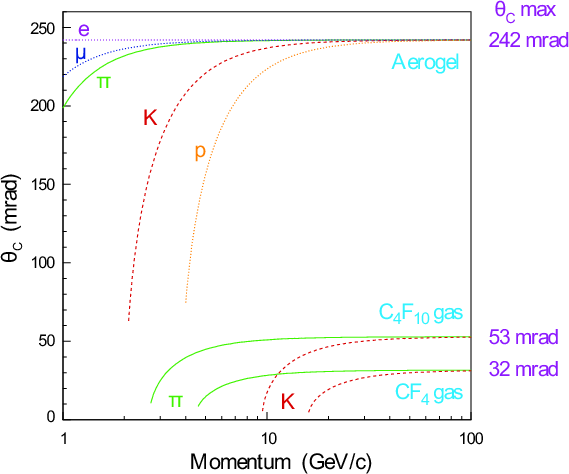
\includegraphics[height=0.3\textheight]{figs/detector/radiators.png}
\caption{Cherenkov angle versus particle momentum for the three gas radiators used in the \rich system.}
\label{fig:radiators}
\end{figure}

The calorimeter system~\cite{LHCb-TDR-002} is used both to identify and to measure the position and energy of photons, electrons and hadrons. It consists of a Scintillating Pad Detector (SPD), a Preshower (PS), an electromagnetic calorimeter (ECAL) and a hadronic calorimeter (HCAL). The ECAL is a scintillator/lead sampling calorimeter with an energy resolution of $\sigma_{E}/\sqrt{E} = 1\% + 10\%/\sqrt{E}$. The HCAL is a scintillator/iron sampling calorimeter with an energy resolution of approximately $\sigma_{E}/\sqrt{E} \sim 70\%/\sqrt{E}$. 

The muon system~\cite{LHCb-TDR-004,muon-tdr2,muon-tdr3,LHCb-DP-2012-002} is used to identify muons and consists of five stations. The first station, M1, is located upstream of the calorimeters and uses triple Gas Electron Multiplier (GEM) detectors. The remaining four stations, M2-M5, located downstream of the calorimeters use Multiwire Proportional Chambers (MWPC) which are interleaved with 80\cm thick iron absorbers to select penetrating muons.

For a given particle hypothesis (\kaon, \pion, \muon, \proton), a combined, overall likelihood is obtained using information from the \rich detectors, the calorimeters and the muon system. The variable commonly used for PID selection requirements is the delta log likelihood (\dll), for example,

\begin{equation}
\dllkpi = \log(\lum_{\kaon}) - \log(\lum_{\pion})
\end{equation}

\noindent where $\lum_{\kaon}$ is the likelihood that the particle is a kaon and $\lum_{\pion}$ is the likelihood that the particle is a pion.
\subsubsection{Trigger system}
\label{detector:trigger}

The \lhcb trigger system~\cite{LHCb-TDR-010,LHCb-DP-2012-004} plays an important role in selecting signal events and reducing the data rate to disk. Two key signatures of the decays of beauty and charm hadrons are large invariant masses and large lifetimes with respect to light unflavoured particles. The large invariant masses result in the daughter particles having significant transverse momentum with respect to the beam axis (\pt). The large lifetimes lead to the daughter particles having a large IP with respect to the primary vertex. Several key channels also contain muons in the final state.

The trigger system consists of two stages: a hardware trigger (\lone) followed by a high-level trigger implemented in software (\hlt). The trigger scheme used in 2012 data taking is shown in Fig.~\ref{fig:trigger:run1}. The L0 trigger reduces the event rate from the rate of visible interactions at $\sim$13\mhz to 1\mhz at which the \lhcb detector can be read out. Therefore, a decision based on information from the muon systems and calorimeters needs to be reached in less than 4\mus. Events that contain high \pt muons or large transverse energy deposits in either calorimeter are selected by L0.

In the first stage of the software trigger (\hltone), a partial event reconstruction is performed due to the limitations of the available computing power. The \hlt is implemented in a online computing farm containing around 29 000 logical cores, giving it approximately 30\ms to process each event~\cite{trigger-cpu}. In order to reduce the execution time of the reconstruction sequence, only \velo track segments that either have a large IP with respect to the primary vertex or are matched to hits in the muon stations are extrapolated into the main tracking system.{\interfootnotelinepenalty=10000\footnote{It should be noted that the IP requirements bias the observable lifetime distributions for fully hadronic \bquark hadron decays.}} The event is selected if a good quality track with a large \pt is found, further reducing the event rate to 70\khz. 

Events selected by \hltone are passed to the second stage of the software trigger (\hlttwo). In this stage, all tracks with a minimum \pt greater than 300\mevc are reconstructed without any requirement on IP or matched muon hits. A combination of exclusive and inclusive selections are used to reduce the event rate to 5\khz, which is written to disk. The inclusive selection of heavy flavour decays with hadrons in the final state is performed by a ``topological'' algorithm containing a multivariate classifier that identifies \bquark hadron decays with two-, three- and four-track vertices~\cite{trigger-inclusive,trigger-topo}.

\begin{figure}[!tb]
\begin{subfigure}{0.49\textwidth}
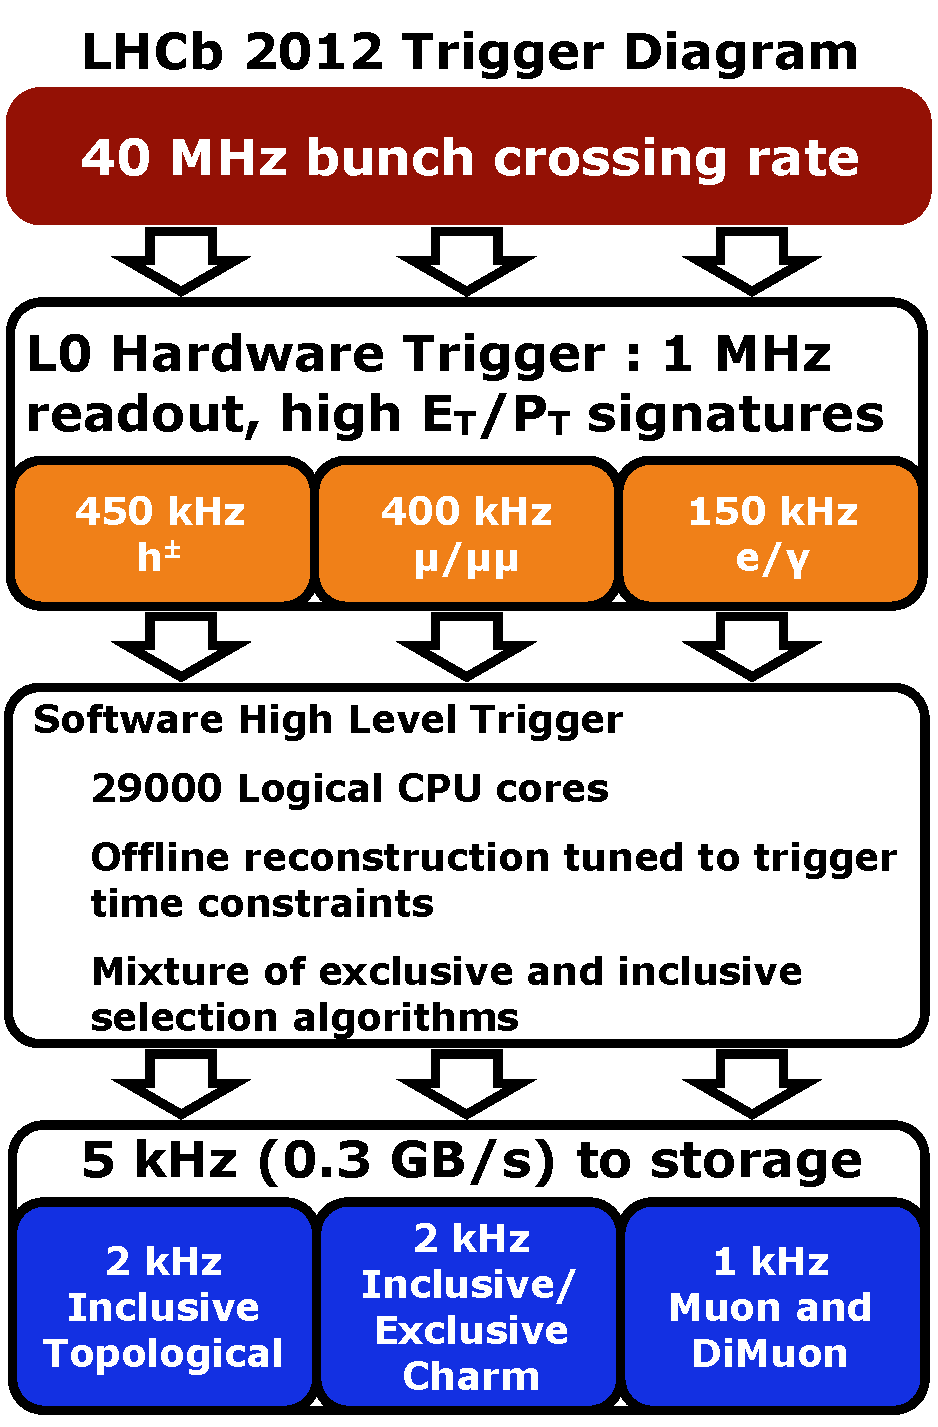
\includegraphics[width=0.9\textwidth]{figs/detector/trigger-run1.pdf}
\caption{}
\label{fig:trigger:run1}
\end{subfigure}
\begin{subfigure}{0.49\textwidth}
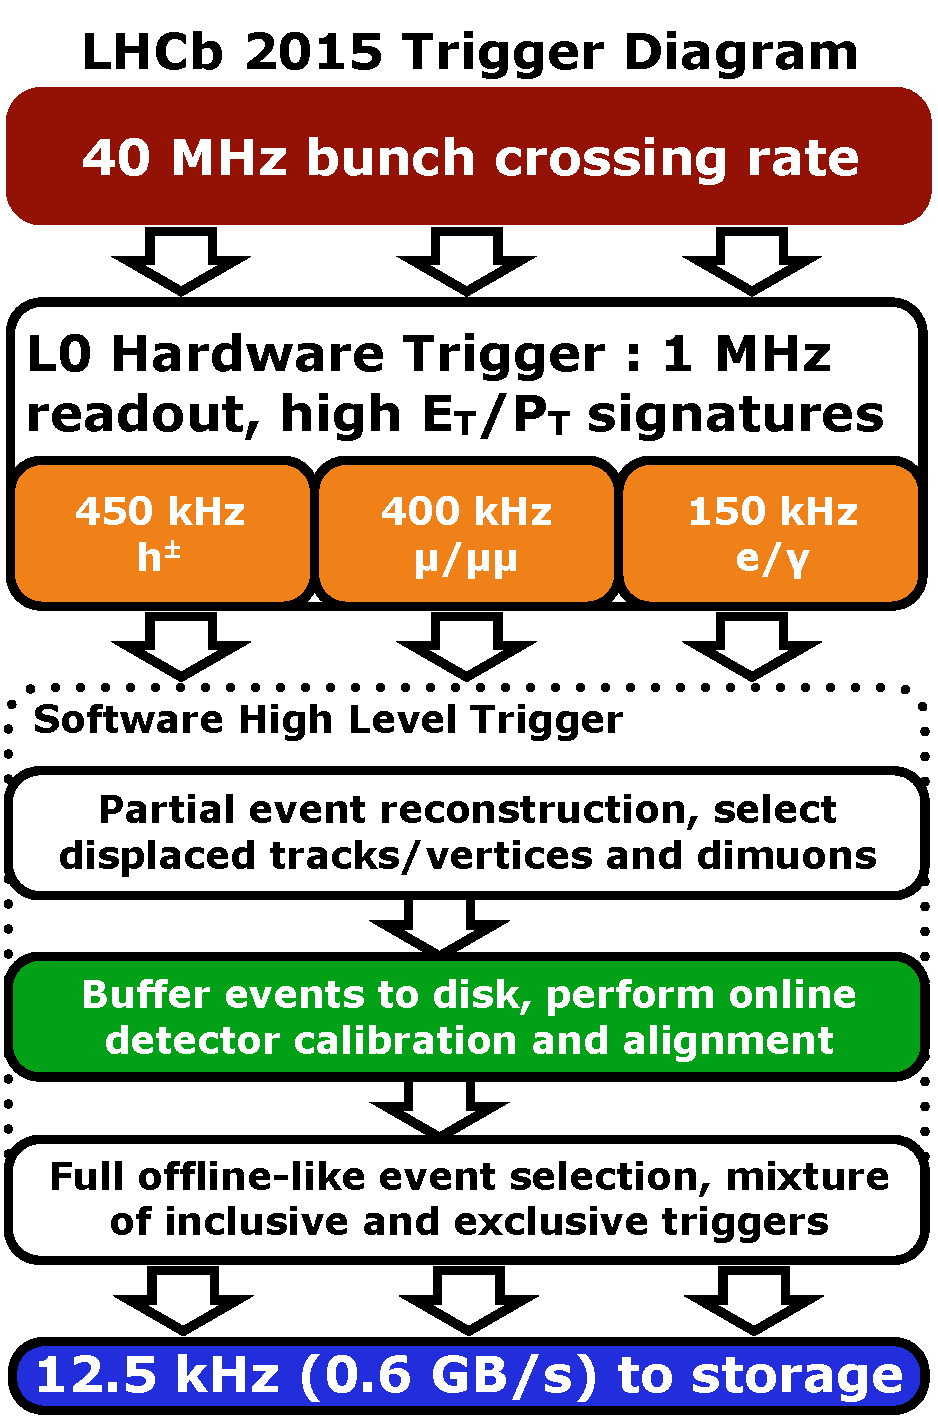
\includegraphics[width=0.9\textwidth]{figs/detector/trigger-run2.pdf}
\caption{}
\label{fig:trigger:run2}
\end{subfigure}
\caption{The trigger schemes used for (a) 2012 and (b) 2015 data taking.}
\label{fig:trigger}
\end{figure}

\subsection{\lhcb Run 2}
\label{sec:lhcb:lhcb-run2}

During Run 2 of the \lhc (2015-2018), the \lhcb experiment has been taking data at an increased center-of-mass energy of \sqs = 13\tev. The bunch spacing has also changed from 50\ns to the design value of 25\ns. With these conditions the same instantaneous luminosity of $4\times10^{32}\cm^{-2}\sec^{-1}$ as for 2012 data taking can be achieved with a lower pile-up. The online computing farm will also be upgraded to include a 5 PB disk buffer. 

The software trigger used in Run 1 contained only a simplified track reconstruction sequence with respect to the one used in the full offline event reconstruction. Furthermore, only a preliminary alignment and calibration of the detector was available and no information from the \rich system was used. For Run 2, the trigger system was redesigned with two key objectives: to enable the full offline event reconstruction to be performed within the trigger and to achieve the same alignment and calibration quality at the trigger level as could be achieved offline during Run 1~\cite{hlt-run2}. These two features allow physics analyses to be performed directly on the output of the software trigger~\cite{turbo}.

The trigger scheme used in 2015 data taking is shown in Fig.~\ref{fig:trigger:run2}. Following the hardware stage and a partial event reconstruction, selected events are buffered to disk. The automatic alignment and calibration procedure is then performed~\cite{alignment}. Once the detector is aligned and calibrated, the full offline-like event reconstruction is performed. With the full information available, including PID from the \rich system, a wide range of inclusive and exclusive selections can be performed in order to trigger the event.

 With the offline quality event reconstruction achieved in the new trigger scheme, it is also possible to only write out the information of the signal candidates~\cite{turbo}. This leads to a large saving in storage space ($\sim 90$\%) and is ideal for the analysis of channels with high yields that would previously have been heavily pre-scaled. It also allows rapid turn-around from data taking to analysis on the order of a few weeks~\cite{LHCb-PAPER-2015-037,LHCb-PAPER-2015-041}. However, this trigger scheme requires careful planning of the selection criteria in order to not leave out potential interesting physics cases.

\subsection{\lhcb Upgrade}
\label{sec:lhcb:lhcb-upgrade}

The \lhcb experiment will undergo an upgrade during Long Shutdown 2 (2018-2019) to allow data taking at \sqs = 14\tev with an instantaneous luminosity of $2\times10^{33}$cm$^{-2}$s$^{-1}$~\cite{upgrade-loi,LHCb-TDR-012}. The upgraded detector will collect at least 5\invfb a year over 10 years of operation.

Two key features of the \lhcb Upgrade are the following: a trigger-less readout system and a full software trigger~\cite{LHCb-TDR-016}. With the current experiment the collision rate must be reduced to the readout rate of 1\mhz. This is achieved using basic information from the calorimeters and muon system as described in Sec.~\ref{detector:trigger}. The largest inefficiencies in the trigger chain, especially for purely hadronic decays, occur at this stage. Furthermore, this constraint inhibits the operation of the detector at higher instantaneous luminosities as trigger yields for hadronic channels would saturate, as shown in Fig.~\ref{fig:upgrade-motivation}. Removing this bottleneck by implementing a trigger-less readout system will allow the full rate of visible interactions to be processed by a purely software trigger. This trigger will offer great flexibility and improve the trigger efficiency significantly for a number of physics channels. %It will also allow lifetime unbiased hadronic triggering for the first time at a hadron collider.

\begin{figure}[!tb]
\centering
\adjincludegraphics[width=0.8\textwidth,trim={{.2\width} {.59\height} {.2\width} {.1\height}},clip]{figs/detector/upgrade-motivation.pdf}
\caption{The trigger yield as a function of instantaneous luminosity for different decays of \B mesons~\cite{upgrade-loi}.}
\label{fig:upgrade-motivation}
\end{figure}

In order to incorporate a trigger-less readout, all the front-end electronics need to be replaced as many sub-detectors cannot currently be read out at 40\mhz. Futhermore, the upgraded detector will need to be able to cope with the factor five increase in instantaneous luminosity. Therefore, many of the existing sub-detectors will be replaced. The current \velo will be replaced by the \velo Pixel (VP) detector~\cite{LHCb-TDR-013}. The VP will contain 41 million $55\times55$\mum pixel sensors with micro-channel \cotwo cooling. When closed, the innermost pixel will be located just 5.1\mm from the \lhc beam. The TT will be replaced by the Upstream Tracker (UT)~\cite{LHCb-TDR-015}, shown schematically in Fig.~\ref{fig:ut}. The UT will be a high granularity silicon microstrip detector with improved coverage of the \lhcb acceptance. The IT and OT will be replaced by the Scintillating Fibre Tracker (SciFi)~\cite{LHCb-TDR-015}. This single, fast detector will contain 2.5\m long multilayer ribbons of 250\mum diameter scintillating fibres with silicon photomultiplier readout.

\begin{figure}[!tb]
\centering
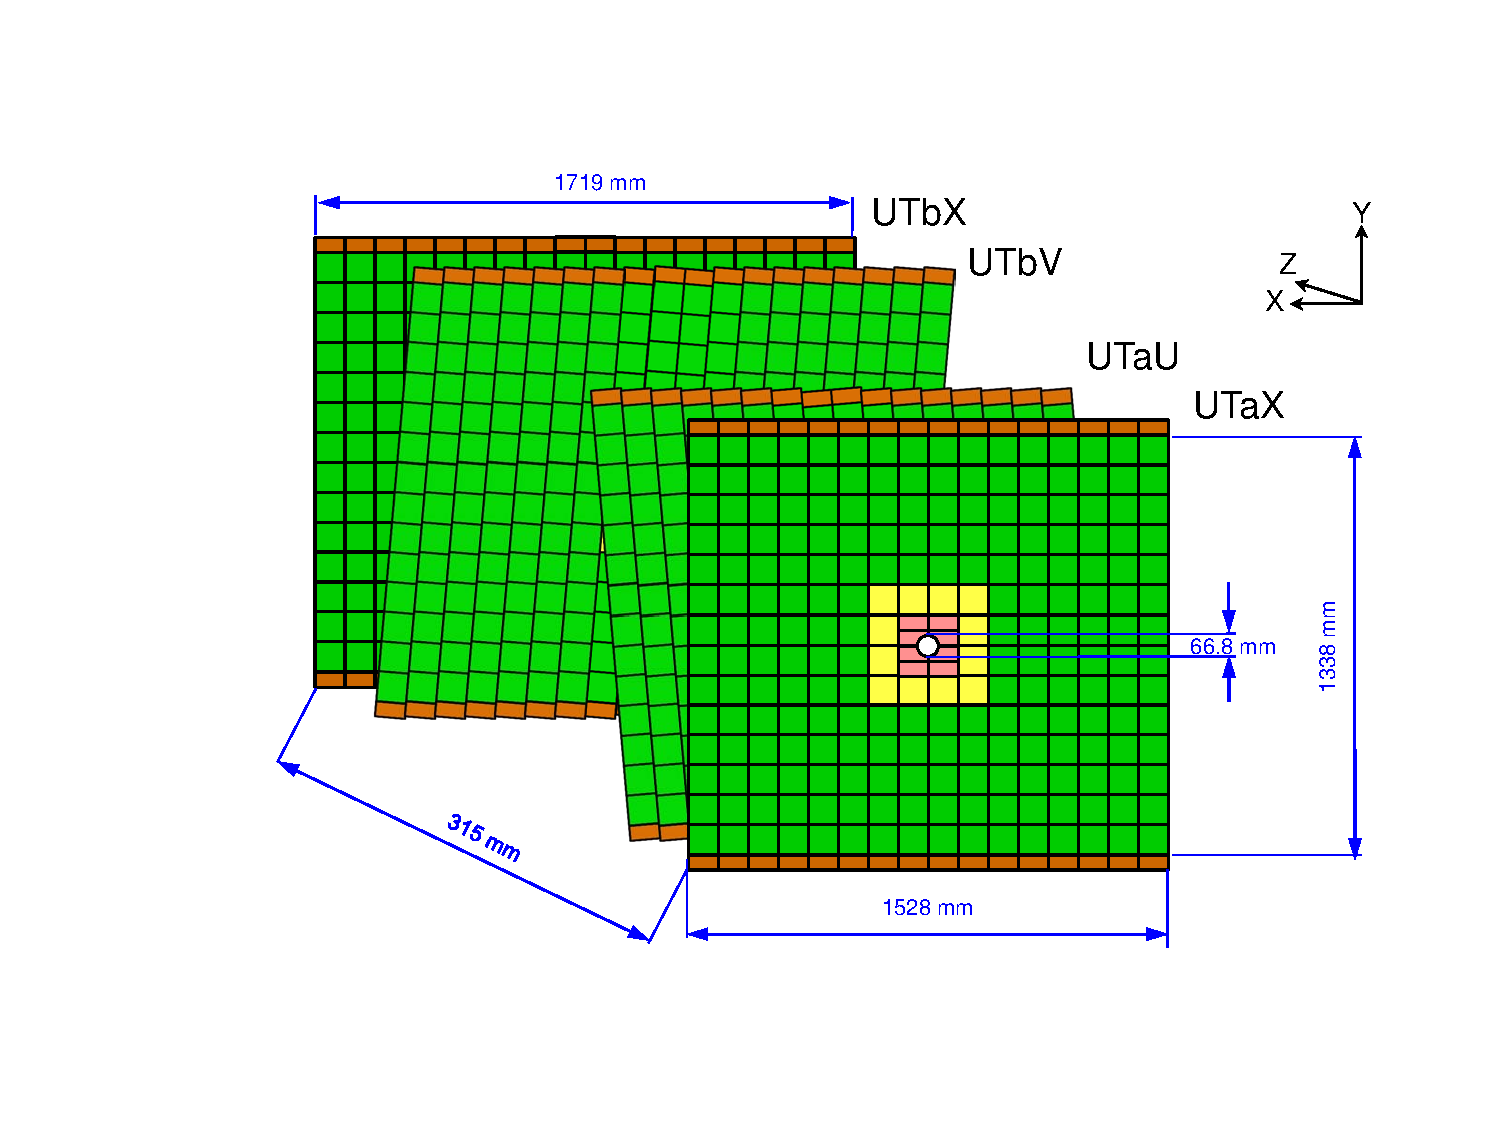
\includegraphics[width=0.8\textwidth]{figs/detector/ut.pdf}
\caption{Schematic view of the UT sub-detector geometry. The different sensor geometries are colour coded.}
\label{fig:ut}
\end{figure}

\clearpage
\section{Track reconstruction}
\label{sec:track}

The track reconstruction in \lhcb is performed by several different algorithms~\cite{tracking}. In order to describe the process, it is first necessary to introduce the notion of track types and track states which are described in Sec.~\ref{sec:track:track-types} and Sec.~\ref{sec:track:track-states} respectively. Each of the tracking algorithms used in Run 1 are described in detail in Sec.~\ref{sec:track:algos} with special emphasis given to the upstream tracking algorithm. The duplicate track removal and track fit procedures are described in Sec.~\ref{sec:track:clone} and Sec.~\ref{sec:track:fit} respectively. Finally, the methods used to determine the performance of the track reconstruction using simulation are detailed in Sec.~\ref{sec:track:performance}.

\subsection{Track types}
\label{sec:track:track-types}

The tracks reconstructed in the \lhcb detector are divided into types depending on the sub-detectors in which they are reconstructed, as shown in Fig.~\ref{fig:track-types}. \velo tracks are defined as those which have measurements only in the \velo sub-detector. These tracks can be either forward or backward. Upstream tracks are defined as those which have measurements only in the \velo and TT (UT) sub-detectors. Upstream tracks are also referred to as \velott(\velout) tracks. T tracks are defined as those which have measurements solely in the T stations. Downstream tracks have measurements in the TT (UT) sub-detector and T stations. Long tracks have measurements in the \velo sub-detector and T stations and may also have measurements in the TT (UT) sub-detector. These tracks provide the best momentum resolution for particles which traverse the full tracking detector and are used in the majority of \lhcb analyses.

\begin{figure}[!tb]
\centering
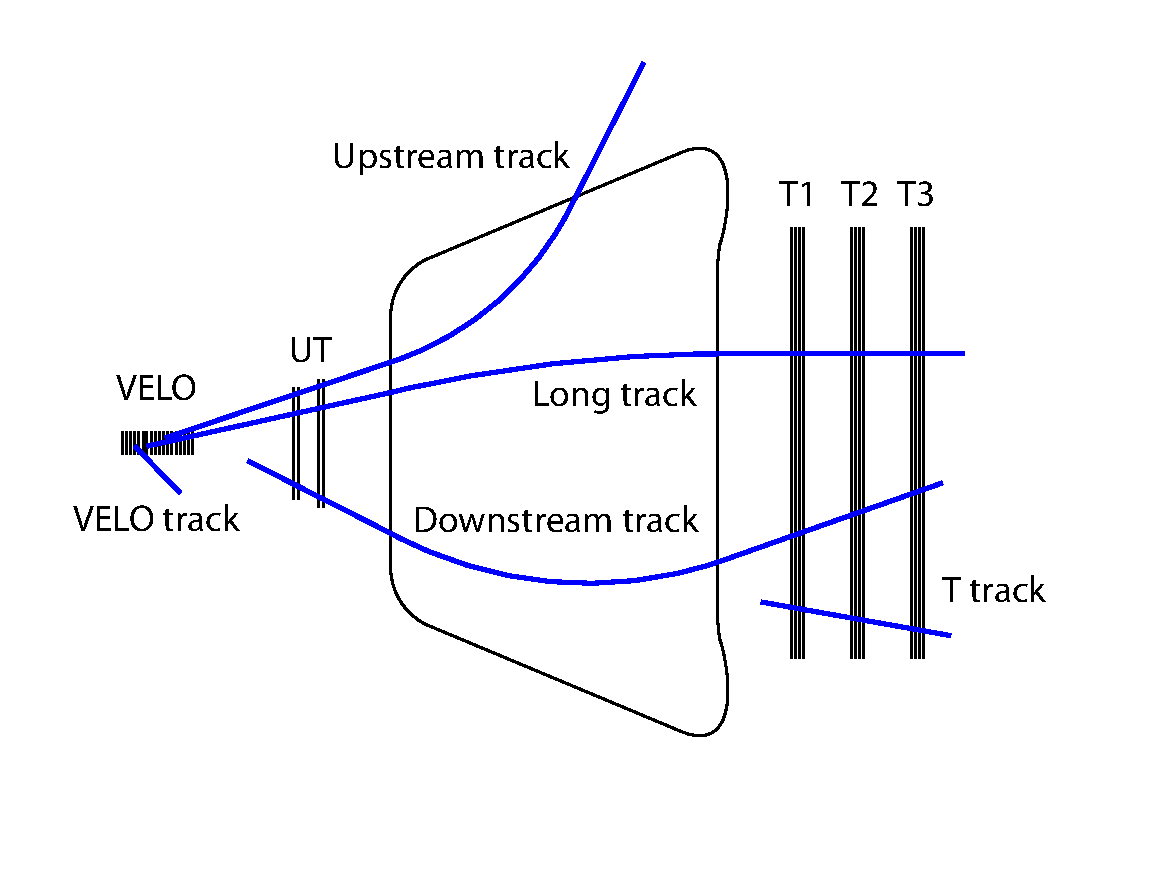
\includegraphics[width=0.8\textwidth]{figs/tracking/trackTypes.pdf}
\caption{Schematic diagram of the \lhcb tracking system. The various track types reconstructed by the different tracking algorithms are shown.}
\label{fig:track-types}
\end{figure}

\subsection{Track states}
\label{sec:track:track-states}

In \lhcb, a track is modelled as a series of straight line segments
called track states. A track state is defined by a state vector of the form

\begin{equation}
\vec x = 
\begin{pmatrix}
x \\
y \\
t_{x} \\
t_{y} \\
q/p \\
\end{pmatrix}
\text{with}~t_{x} = \frac{\partial x}{\partial z} ~\text{and}~ t_{y} = \frac{\partial y}{\partial z} 
\end{equation}

\noindent and a corresponding $5\times5$ state covariance matrix at a given position in $z$. Here, $q$ and $p$ are the charge and momentum of the track respectively.

\subsection{Track reconstruction algorithms}
\label{sec:track:algos}

In order to reconstruct the different track types, several tracking algorithms are employed. The two stand-alone algorithms, \velo tracking and track seeding, are described in Sec.~\ref{sec:track:algos:velo} and Sec.~\ref{sec:track:algos:seeding} respectively. The other algorithms use input from these two algorithms in order to perform a further track reconstruction.

\subsubsection{\velo tracking}
\label{sec:track:algos:velo}

The \velo tracking algorithm~\cite{fastvelo} is used to find tracks in the \velo. As there is a neglible magnetic field in the \velo, tracks are expected to be approximately straight lines. The track search begins in the most downstream layer of the \velo. Quadruplets of hits are searched for in the $r$-sensors as shown in Fig.~\ref{fig:velo-tracking}. If they are found, they are extended back to smaller $z$ adding hits that are consistent with coming from the same track. Next, the same quadruplet search is performed for backward-going tracks. Triplets are then searched for, first backward-going and then forward-going, requiring that the hits have not been used in the quadruplet search.

Starting from the longest $r$-$z$ track, $\phi$ hits are searched for that are consistent with coming from the same track. These 3D tracks are then fitted with a $\chi^{2}$ minimization.

\begin{figure}[!tb]
  \centering
  \resizebox{\columnwidth}{!}{
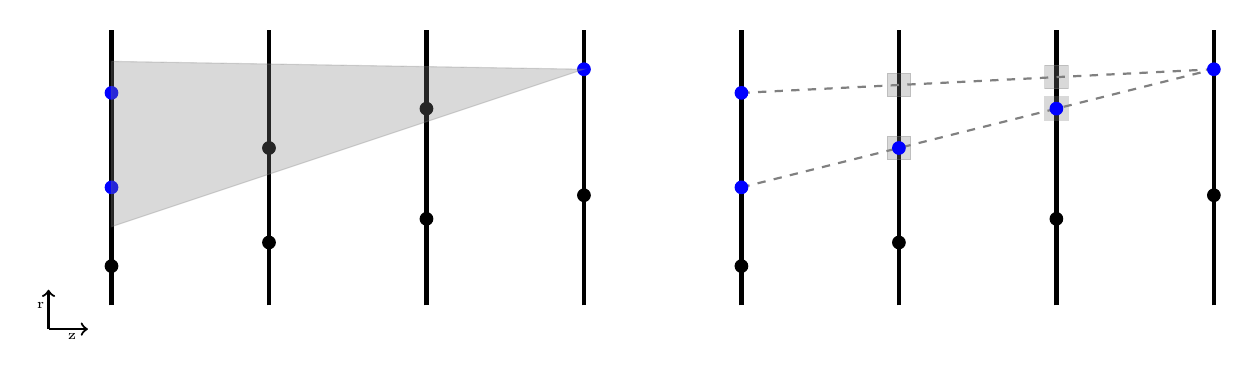
\begin{tikzpicture}
  %\draw[step=1cm,gray,very thin] (0,0) grid (15,4.5);
  \draw[ultra thick] (1.,0.5) -- (1.,4);
  \draw[ultra thick] (3,0.5) -- (3,4);
  \draw[ultra thick] (5,0.5) -- (5,4);
  \draw[ultra thick] (7,0.5) -- (7,4);
  
  \draw[fill,blue] (7,3.5) circle (0.08);
  \draw[fill,blue] (1,2) circle (0.08);
  \draw[fill] (3,2.5) circle (0.08);
  \draw[fill] (5,3) circle (0.08);
  
  \draw[fill] (1,1.) circle (0.08);
  \draw[fill] (3,1.3) circle (0.08);
  \draw[fill] (5,1.6) circle (0.08);
  \draw[fill] (7,1.9) circle (0.08);
  
  \draw[fill,blue] (1,3.2) circle (0.08);
  
  \draw[fill,gray,opacity=0.3] (7,3.5)--(1,1.5)--(1,3.6)--cycle;
  
  \draw[ultra thick] (9.,0.5) -- (9.,4);
  \draw[ultra thick] (11,0.5) -- (11,4);
  \draw[ultra thick] (13,0.5) -- (13,4);
  \draw[ultra thick] (15,0.5) -- (15,4);
  
  \draw[thick,gray, dashed] (9,2) -- (15,3.5);
  \draw[thick,gray, dashed] (9,3.2) -- (15,3.5);
  
  \draw[fill,gray,opacity=0.3] (10.85,2.35) rectangle (11.15,2.65);
  \draw[fill,gray,opacity=0.3] (12.85,2.85) rectangle (13.15,3.15);
  
  \draw[fill,gray,opacity=0.3] (10.85,3.15) rectangle (11.15,3.45);
  \draw[fill,gray,opacity=0.3] (12.85,3.25) rectangle (13.15,3.55);
  
  \draw[fill,blue] (15,3.5) circle (0.08);
  \draw[fill,blue] (9,2) circle (0.08);
  \draw[fill,blue] (11,2.5) circle (0.08);
  \draw[fill,blue] (13,3) circle (0.08);
  
  \draw[fill] (9,1.) circle (0.08);
  \draw[fill] (11,1.3) circle (0.08);
  \draw[fill] (13,1.6) circle (0.08);
  \draw[fill] (15,1.9) circle (0.08);
  
  \draw[fill,blue] (9,3.2) circle (0.08);
  
  \draw[thick,->] (0.2,0.2) -- (0.7,0.2);
  \draw[thick,->] (0.2,0.2) -- (0.2,0.7);
  
  \node[draw=none] at (0.5,0.1){\tiny z};
  \node[draw=none] at (0.1,0.5){\tiny r};
  
\end{tikzpicture}
}
  \caption{Quadruplets of hits are searched for in the \velo starting from the most downstream layer. Starting with a hit in that layer, a search window is opened in the fourth most downstream layer. From hits found within the window, the expected position of hits in the intermediate layers can be predicted assuming the track is a straight line in the $r$-$z$ projection. If hits fall within a tolerance of the expected positions, quadruplets are formed and a track is created.}
  \label{fig:velo-tracking}
\end{figure}

\subsubsection{Forward tracking}
\label{sec:track:algos:forward}

The Forward tracking algorithm~\cite{patforward} is used to find long tracks. A Hough transform is utilised to associate hits in the T-stations to each \velo track. The \velo track is linearly extrapolated to the T-stations and a symmetric search window is opened in each $x$ layer. The VELO track state and knowledge of the $\vec{B}$ field are used to project each selected hit to the $z$ position of a reference plane. Hits from the same particle are expected to be projected to the same $x$ position while random hits should be uniformly distributed. This procedure is shown schematically in Fig.~\ref{fig:forward-tracking}. The resulting clusters are fitted and outliers are removed using a $\chi^{2}$ criterium. An additional cluster search is used to add stereo hits that are consistent with the $x$-$z$ track. This 3D track is then fitted, outliers are removed and the best track candidate is chosen based on its $\chi^{2}$/dof.

\begin{figure}[!tb]
  \centering
  \resizebox{\columnwidth}{!}{
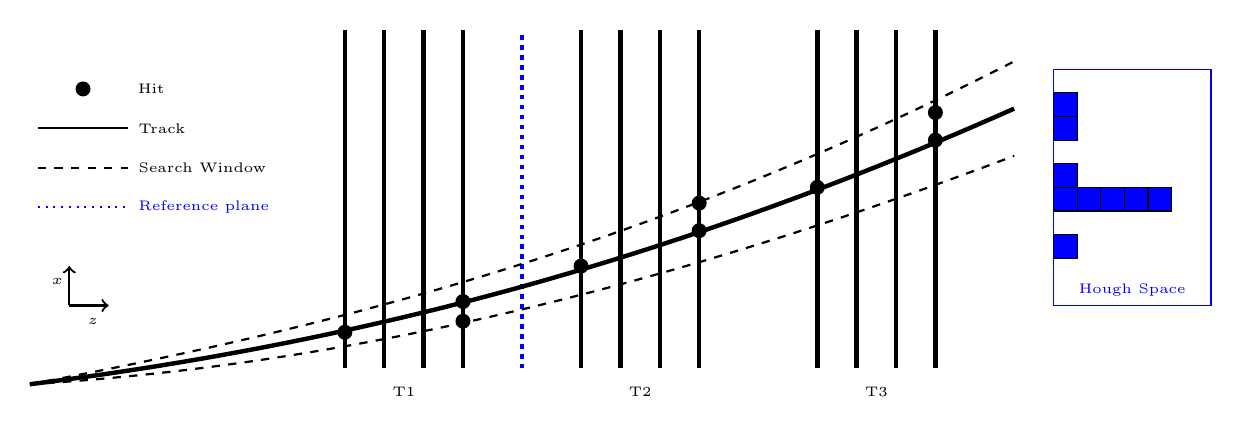
\begin{tikzpicture}
  %\draw[step=1cm,gray,very thin] (0,0) grid (15,5.);
    
  \draw[thick,->] (0.5,1) -- (0.5,1.5);
  \draw[thick,->] (0.5,1) -- (1.,1);
  \node[draw=none] at (0.35,1.3){\tiny $x$};
  \node[draw=none] at (0.8,0.8){\tiny $z$};
  
  \draw[ultra thick] (4,0.2) -- (4,4.5);
  \draw[ultra thick] (4.5,0.2) -- (4.5,4.5);
  \draw[ultra thick] (5,0.2) -- (5,4.5);
  \draw[ultra thick] (5.5,0.2) -- (5.5,4.5);

  \draw[ultra thick] (7,0.2) -- (7,4.5);
  \draw[ultra thick] (7.5,0.2) -- (7.5,4.5);
  \draw[ultra thick] (8,0.2) -- (8,4.5);
  \draw[ultra thick] (8.5,0.2) -- (8.5,4.5);

  \draw[ultra thick] (10,0.2) -- (10,4.5);
  \draw[ultra thick] (10.5,0.2) -- (10.5,4.5);
  \draw[ultra thick] (11,0.2) -- (11,4.5);
  \draw[ultra thick] (11.5,0.2) -- (11.5,4.5);

  \draw[dotted,blue,ultra thick] (6.25,0.2) -- (6.25,4.5);
  
  \draw[ultra thick] (0,0.0)  .. controls (4,0.5)  and (8,1.5) .. (12.5,3.5);
  \draw[thick,dashed] (0,0.0)  .. controls (4,0.25)  and (8,1.2) .. (12.5,2.9);
  \draw[thick,dashed] (0,0.0)  .. controls (4,0.75)  and (8,1.8) .. (12.5,4.1);
  
  \draw[fill] (4,0.66) circle [radius=2.5pt];
  \draw[fill] (5.5,1.05) circle [radius=2.5pt];

  \draw[fill] (7,1.5) circle [radius=2.5pt];
  \draw[fill] (8.5,1.95) circle [radius=2.5pt];

  \draw[fill] (10,2.5) circle [radius=2.5pt];
  \draw[fill] (11.5,3.1) circle [radius=2.5pt];

  \draw[fill] (5.5,0.8) circle [radius=2.5pt];
  \draw[fill] (8.5,2.3) circle [radius=2.5pt];
  \draw[fill] (11.5,3.45) circle [radius=2.5pt];
  
  \draw (13,1)[blue] rectangle (15,4);
  \node[draw=none,blue] at (14.0,1.2){\tiny Hough Space};
  \fill[blue,draw=black] (13,2.2) rectangle (13.3,2.5);
  \fill[blue,draw=black] (13.3,2.2) rectangle (13.6,2.5);
  \fill[blue,draw=black] (13.6,2.2) rectangle (13.9,2.5);
  \fill[blue,draw=black] (13.9,2.2) rectangle (14.2,2.5);
  \fill[blue,draw=black] (14.2,2.2) rectangle (14.5,2.5);
  \fill[blue,draw=black] (13.0,2.5) rectangle (13.3,2.8);
  

  \fill[blue,draw=black] (13,1.6) rectangle (13.3,1.9);
  
  \fill[blue,draw=black] (13.0,3.1) rectangle (13.3,3.4);
  \fill[blue,draw=black] (13,3.4) rectangle (13.3,3.7);
  
  \draw[white] (0.1,3.75) -- (1.25,3.75) node[anchor=west] {\tiny \textcolor{black}{Hit}};
  \draw[fill] (0.675,3.75) circle [radius=2.5pt];
  \draw[thick] (0.1,3.25) -- (1.25,3.25) node[anchor=west] {\tiny Track};
  \draw[thick,dashed] (0.1,2.75) -- (1.25,2.75) node[anchor=west] {\tiny Search Window};
  \draw[thick,dotted,blue,text opacity=1] (0.1,2.25) -- (1.25,2.25) node[anchor=west] {\tiny Reference plane};
  
  \node[draw=none] at (4.75,-0.1){\tiny T1};
  \node[draw=none] at (7.75,-0.1){\tiny T2};
  \node[draw=none] at (10.75,-0.1){\tiny T3};
  
\end{tikzpicture}
}
  \caption{A Hough transform is used to associate hits in the T-stations to a \velo track. Each hit within a search window around the extrapolated track is projected to the $z$ position of a reference plane. Hits from the same particle are expected to be projected to the same $x$ position while random hits should be uniformly distributed.}
  \label{fig:forward-tracking}
\end{figure}

\subsubsection{T seeding}
\label{sec:track:algos:seeding}

The T seeding algorithm~\cite{patseeding} is used to find T tracks. Track candidates are first searched for in the $x$-$z$ projection. A straight line is formed between suitable pairs of hits in T1 and T3. A compatible hit in T2 is added to form a parabola. Further hits in $x$ layers consistent with this parabola are added to the track candidate. A Hough transform is used to add stereo hits. A weighted least squares fit is then applied to each candidate.

\subsubsection{Track matching}
\label{sec:track:algos:match}

The track matching algorithm~\cite{patmatch} is also used to form long tracks. It takes both \velo and T tracks as input (seeds). The difference in $x$ and $y$ of the two seeds are calculated by extrapolating them both to the magnet bending plane ($\Delta x$) and the end of the T-stations ($\Delta y$) respectively. A matching criterion $\chi^{2}$ is formed using $\Delta x$, $\Delta y$, $\Delta t_{x}$ and $\Delta t_{y}$. If the track passes this criterion it is fitted and an estimate is made of its $q/p$.

\subsubsection{Downstream tracking}
\label{sec:track:algos:downstream}

The downstream tracking algorithm~\cite{patdownstream,sascha} forms tracks containing hits in the TT(UT) sub-detector and T stations. Each T track is extrapolated back to find the corresponding ($x$, $y$) point at the center of the magnet. A track estimate is formed using this point and the nominal interaction point. Hits in the TT consistent with the track estimate are selected. For each TT hit, a new track estimate is formed and consistent $x$ hits are collected. The collection of $x$ hits is fitted in the $x$-$z$ projection and outliers are removed. Stereo hits are added, the track is refitted and further outliers are removed. Finally, the best track candidate is chosen according to the number of hits it contains and the value of the $\chi^{2}$ from the fit.


\subsubsection{Upstream tracking}
\label{sec:track:algos:upstream}

The upstream tracking algorithm~\cite{patvelott} forms tracks containing hits in the \velo and TT(UT) sub-detectors. These are generally low momentum tracks that will be bent out of acceptance by the magnet. It is executed at the end of the tracking sequence using \velo tracks which have not been upgraded to long tracks by any of the preceeding algorithms. 

Each \velo track is linearly extrapolated to the TT. Search windows are opened in each layer and the distance $\Delta x$ between the track and each hit is calculated. These $\Delta x$ values are scaled to a reference plane at the center of the TT. A Hough transform is utilised to associate the selected hits to the \velo track. Hits from the same particle are expected to be projected to the same $x$ position in the reference plane while random hits should be uniformly distributed. This procedure is shown schematically in Fig.~\ref{fig:velott-tracking}. An explicit assumption is made that every associated hit should lie on the same side of the extrapolated \velo track in the $x$-$z$ plane. 

 Each track candidate is fitted with a simplified $\chi^{2}$ minimisation and the $q/p$ of the track is estimated. Due to the fringe $\vec{B}$ field between the \velo and the TT a momentum estimate of $\delta p/p \sim~15\%$ is possible. The best track candidate is chosen based on the number of TT layers containing hits and the $\chi^{2}$ of the simplified fit. Each of the \velott tracks is subsequently fitted with a Kalman filter, described in Sec.~\ref{sec:track:fit}, in order to obtain the most accurate estimates of track parameters along with their corresponding covariance matrices.

\begin{figure}[!tb]
  \centering
  \resizebox{\columnwidth}{!}{
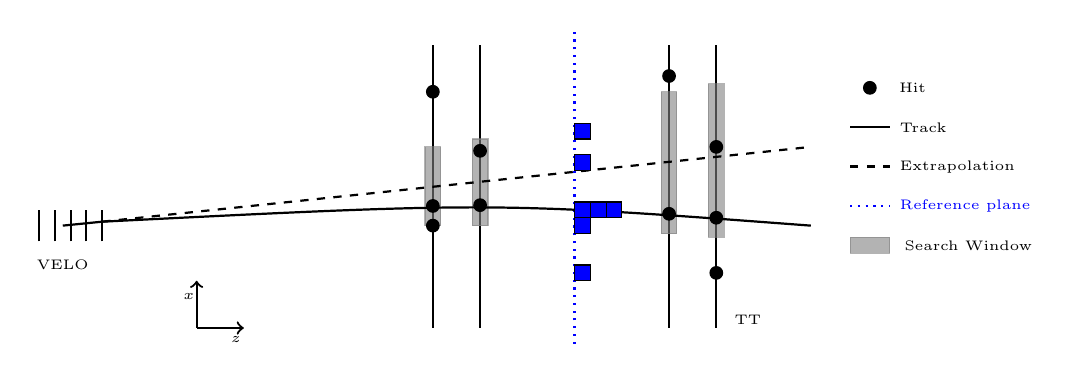
\begin{tikzpicture}
  %\draw[step=1cm,gray,very thin] (0,0) grid (13,4);

  \draw[thick,->] (2.2,0.2) -- (2.2,0.8);
  \draw[thick,->] (2.2,0.2) -- (2.8,0.2);
  \node[draw=none] at (2.1,0.6){\tiny $x$};
  \node[draw=none] at (2.7,0.05){\tiny $z$};

  \draw[thick] (0.2,1.3) -- (0.2,1.7);
  \draw[thick] (0.4,1.3) -- (0.4,1.7);
  \draw[thick] (0.6,1.3) -- (0.6,1.7);
  \draw[thick] (0.8,1.3) -- (0.8,1.7);
  \draw[thick] (1.0,1.3) -- (1,1.7);

  \draw[thick] (5.2,0.2) -- (5.2,3.8);
  \draw[thick] (5.8,0.2) -- (5.8,3.8);
  \draw[thick] (8.2,0.2) -- (8.2,3.8);
  \draw[thick] (8.8,0.2) -- (8.8,3.8);

  \draw[thick,dotted,blue] (7,0) -- (7,4);

  \draw[fill,gray,opacity=0.6] (5.1,1.5) rectangle (5.3,2.5);
  \draw[fill,gray,opacity=0.6] (5.7,1.5) rectangle (5.9,2.6);
  \draw[fill,gray,opacity=0.6] (8.1,1.4) rectangle (8.3,3.2);
  \draw[fill,gray,opacity=0.6] (8.7,1.35) rectangle (8.9,3.3);
  
  \draw[thick] (0.5,1.5) -- (1,1.5+0.5*0.1);
  \draw[thick,dashed] (1,1.5+0.5*0.1) -- (10,1.5+10*0.1);
  \draw[thick] (1,1.5+0.5*0.1) .. controls (6,1.8) .. (10,1.5);

  \draw[fill] (5.2,1.75) circle (0.08);
  \draw[fill] (5.8,1.76) circle (0.08);
  \draw[fill] (8.2,1.65) circle (0.08);
  \draw[fill] (8.8,1.6) circle (0.08);

  \draw[fill] (5.2,1.5) circle (0.08);
  \draw[fill] (5.2,3.2) circle (0.08);
  \draw[fill] (5.8,2.45) circle (0.08);
  \draw[fill] (8.2,3.4) circle (0.08);
  \draw[fill] (8.8,2.5) circle (0.08);
  \draw[fill] (8.8,0.9) circle (0.08);

  \fill[blue,draw=black] (7.0,1.6) rectangle (7.2,1.8);
  \fill[blue,draw=black] (7.2,1.6) rectangle (7.4,1.8);
  \fill[blue,draw=black] (7.4,1.6) rectangle (7.6,1.8);
  \fill[blue,draw=black] (7.0,1.4) rectangle (7.2,1.6);

  \fill[blue,draw=black] (7.0,0.8) rectangle (7.2,1.);
  \fill[blue,draw=black] (7.0,2.2) rectangle (7.2,2.4);
  \fill[blue,draw=black] (7.0,2.6) rectangle (7.2,2.8);

  \node[draw=none] at (0.5,1){\tiny VELO};
  \node[draw=none] at (9.2,0.3){\tiny TT};

  %\draw[thick] (10.5,3.25) -- (11.,3.25)  node[anchor=west] {\tiny Track};
  %\draw[fill] (11.,3.25) circle [radius=2pt]  node[anchor=west] {\tiny Hit};
  \draw[white] (10.5,3.25) -- (11.,3.25)  node[anchor=west] {\tiny \textcolor{black}{Hit}};
  \draw[fill] (10.75,3.25) circle (0.08);
  \draw[thick] (10.5,2.75) -- (11.,2.75)  node[anchor=west] {\tiny Track};
  \draw[thick,dashed] (10.5,2.25) -- (11.,2.25)  node[anchor=west] {\tiny Extrapolation};
  \draw[thick,dotted,blue] (10.5,1.75) -- (11.,1.75)  node[anchor=west] {\tiny Reference plane};
  \draw[fill,gray,opacity=0.6] (10.5,1.15) rectangle (11.0,1.35);
  \node[draw=none] at (12.0,1.25){\tiny Search Window};
\end{tikzpicture}
}

  \caption{A Hough transform is utilised to associate the selected TT hits to the \velo track. Hits from the same particle are expected to be projected to the same $x$ position in the reference plane while random hits should be uniformly distributed.}
  \label{fig:velott-tracking}
\end{figure}

\subsection{Clone removal}
\label{sec:track:clone}

As there are two independent algorithms to produce long tracks and several track types are subtracks of other types, it is necessary to avoid or remove duplicate tracks found by multiple algorithms. This is accounted for in two different ways. Some algorithms are only allowed to use tracks or hits that have not been previously used. When there is a significant overlap of hits between two tracks, the track with the smaller number of hits is discarded. 

\subsection{Track fit}
\label{sec:track:fit}

The purpose of the track fit  is to obtain the most accurate estimates of track parameters along with their corresponding covariances. Track parameters are used to match to particle identification objects (e.g. Cherenkov rings), find primary and secondary vertices and calculate the kinematics and invariant masses of particle combinations. The track $\chi^{2}$ is used to select good quality tracks. 

A Kalman filter is used to fit the tracks. With this approach, multiple scattering is taken into account as process noise and corrections due to energy losses are applied~\cite{kalman}. The transport through the magnetic field is evaluated using a Runge-Kutta method. The propagation and projection functions are linearised around a reference track state using a Taylor expansion~\cite{jeroen}.

Track candidates can be considered as a collection of track states (initially provided by the individual tracking algorithms) and measurements (tracking station hits). The Kalman filter can be divided into two steps, shown schematically in Fig.~\ref{fig:kalman}. Firstly, the parameters of a state at $z_{k}$ are predicted given a state at $z_{k-1}$. Next, the state at $z_{k}$ is updated with information of the measurement at this position. These two steps are repeated until all the measurements have been added. In \lhcb the filter is run in both the forward and the backward directions and the average is taken for smoothing.

\begin{figure}[!tb]
  \centering
  \resizebox{\columnwidth}{!}{
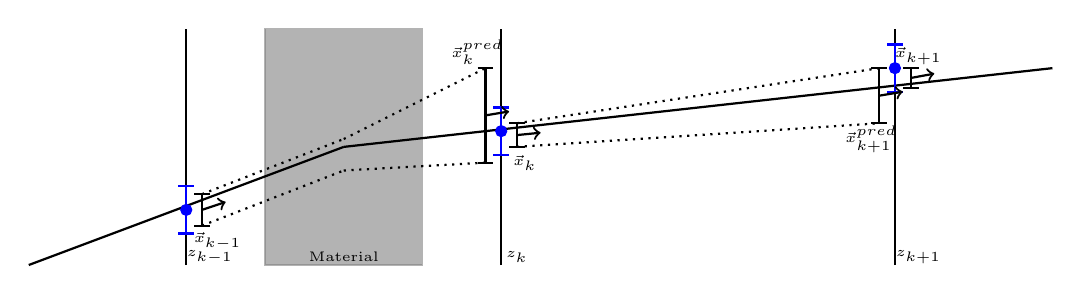
\begin{tikzpicture}
  %\draw[step=1cm,gray,very thin] (0,0) grid (14,3);
  
  \draw[fill,gray,opacity=0.6] (3,0) rectangle (5,3);
  
  \draw[thick] (2,0) -- (2,3);
  \draw[thick] (6,0) -- (6,3);
  \draw[thick] (11,0) -- (11,3);

  \draw[thick] (0,0.) -- (4,1.5);
  \draw[thick] (4,1.5) -- (13,2.5);

  %point 1
  \draw[fill,blue] (2,0.7) circle [radius=2pt];
  \draw[thick,blue] (2,0.4) -- (2,1.);
  \draw[thick,blue] (1.9,0.4) -- (2.1,0.4);
  \draw[thick,blue] (1.9,1.) -- (2.1,1.);

  %point 2
  \draw[fill,blue] (6,1.7) circle [radius=2pt];
  \draw[thick,blue] (6,1.4) -- (6,2.);
  \draw[thick,blue] (5.9,1.4) -- (6.1,1.4);
  \draw[thick,blue] (5.9,2.) -- (6.1,2.);

  %point 3
  \draw[fill,blue] (11,2.5) circle [radius=2pt];
  \draw[thick,blue] (11,2.2) -- (11,2.8);
  \draw[thick,blue] (10.9,2.2) -- (11.1,2.2);
  \draw[thick,blue] (10.9,2.8) -- (11.1,2.8);

  %state 1
  \draw[thick] (2.2,0.5) -- (2.2,0.9);
  \draw[thick] (2.1,0.5) -- (2.3,0.5);
  \draw[thick] (2.1,0.9) -- (2.3,0.9);
  \draw[thick,->] (2.2,0.7) -- (2.5,0.8);

  % state 2 pred
  \draw[thick] (5.8,1.3) -- (5.8,2.5);
  \draw[thick] (5.7,1.3) -- (5.9,1.3);
  \draw[thick] (5.7,2.5) -- (5.9,2.5);
  \draw[thick,->] (5.8,1.9) -- (6.1,1.95);

  % state 2 
  \draw[thick] (6.2,1.5) -- (6.2,1.8);
  \draw[thick] (6.1,1.5) -- (6.3,1.5);
  \draw[thick] (6.3,1.8) -- (6.1,1.8);
  \draw[thick,->] (6.2,1.65) -- (6.5,1.68);

  % state 3 pred 
  \draw[thick] (10.8,1.8) -- (10.8,2.5);
  \draw[thick] (10.7,1.8) -- (10.9,1.8);
  \draw[thick] (10.7,2.5) -- (10.9,2.5);
  \draw[thick,->] (10.8,2.15) -- (11.1,2.2);

  % state 3 
  \draw[thick] (11.2,2.25) -- (11.2,2.5);
  \draw[thick] (11.1,2.25) -- (11.3,2.25);
  \draw[thick] (11.1,2.5) -- (11.3,2.5);
  \draw[thick,->] (11.2,2.375) -- (11.5,2.43);

  \draw[thick,dotted] (2.2,0.9) -- (4,1.6);
  \draw[thick,dotted] (2.2,0.5) -- (4,1.2);
  \draw[thick,dotted] (4,1.6) -- (5.8,2.5);
  \draw[thick,dotted] (4,1.2) -- (5.8,1.3);
  \draw[thick,dotted] (6.2,1.8) -- (10.8,2.5);
  \draw[thick,dotted] (6.2,1.5) -- (10.8,1.8);

  \node[draw=none] at (2.3,0.1){\tiny $z_{k-1}$};
  \node[draw=none] at (6.2,0.1){\tiny $z_{k}$};
  \node[draw=none] at (11.3,0.1){\tiny $z_{k+1}$};

  \node[draw=none] at (2.4,0.3){\tiny $\vec{x}_{k-1}$};
  \node[draw=none] at (5.7,2.7){\tiny $\vec{x}_{k}^{pred}$};
  \node[draw=none] at (6.3,1.3){\tiny $\vec{x}_{k}$};
  \node[draw=none] at (10.7,1.6){\tiny $\vec{x}_{k+1}^{pred}$};
  \node[draw=none] at (11.3,2.65){\tiny $\vec{x}_{k+1}$};

  \node[draw=none] at (4,0.1){\tiny Material};
        
    \end{tikzpicture}
}
  \caption{A schematic diagram of the Kalman filter showing the prediction of a state $z_{k}$ given a state at $z_{k-1}$. The state is at $z_{k}$ is subsequently updated with information of the measurement at this position. This process is repeated until all measurements have been added.}
  \label{fig:kalman}
\end{figure}

\subsection{Tracking performance}
\label{sec:track:performance}

The figures of merit used to evaluate the performance of tracking algorithms are the reconstruction efficiency, ghost rate and execution time and are determined using simulated events. The simulated samples used in the following sections to benchmark the performance of the upstream tracking algorithms for both the \lhcb Upgrade and \lhcb Run 2 are shown in Table~\ref{tab:track-mc-samples}.

\begin{table}[!tb]
\caption{The simulated samples used in the following sections to benchmark the performance of the upstream tracking algorithms for both the \lhcb Upgrade and \lhcb Run 2.}
\begin{center}
\begin{tabular}{c|c|c|c|c}
  & Decay Mode & $\sqrt{s}$~[\tev] & $\nu$ & Bunch spacing~[\ns] \\ 
  \hline
  Run 2 & \BsToPhiPhi, min. bias & 13 & 1.9 & 25 \\
  Upgrade & \BdToKstmm, min. bias & 14 & 7.6 & 25 \\
  \end{tabular}
\end{center}
\label{tab:track-mc-samples}
\end{table}

\subsubsection{Reconstruction efficiency}
\label{sec:track:eff}
The reconstruction efficiency is measured by comparing the number of correctly reconstructed tracks with the number of tracks defined to be reconstructible. This is made possible using truth information available in simulated samples. Within the \lhcb framework the following definitions are used:

\begin{itemize}

\item A particle is reconstructible as a \velo track if there are hits associated to it in at least three $r$ and three $\phi$ \velo sensors.

\item A particle is reconstructible as a long track if it fulfils the requirements to be reconstructible in both the \velo sub-detector and the T stations.

\item A particle is considered reconstructed if at least 70\% of both the \velo and T station hits on a track are associated to it and the track has no more than 1 wrongly associated TT (UT) hit.

\end{itemize}

\noindent The reconstruction efficiency is defined as

\begin{equation}
\epsilon_{rec} = \frac{N_{\text{reconstructible~and~reconstructed}}}{N_{\text{reconstructible}}}.
\end{equation}

When calculating the efficiency of the \velott (\velout) algorithm itself, particles are required to be reconstructible as a long track, have been correctly reconstructed in the \velo and have a matched TT (UT) hit in at least 3 TT (UT) layers. 

When considering the effect of using \velott (\velout) tracks as input to the Forward algorithm, no requirement is made that the particle has associated TT (UT) hits or has been correctly reconstructed in the \velo. Therefore, any inefficiency contains contributions from both the \velott (\velout) algorithm and the acceptance of the TT (UT) detector. 

In this thesis, further requirements are made to both the numerator and the denominator:

\begin{itemize}
\item The particle is required not to be an electron.
\item The pseudorapidity of the particle must lie between 2 and 5.
\item The particle is required to be \bquark hadron daughter.
\item The particle must have \pt\textgreater~0.5\gevc.
\end{itemize}

\noindent These requirements are chosen as \bquark hadrons with a large \pt that decay within the \lhcb acceptance are of foremost interest within the context of the \lhcb software trigger. Electrons are neglected when studying track reconstruction efficiencies, as they are more challenging to reconstruct due to Bremsstrahlung.

\subsubsection{Ghost rate and clone tracks}
\label{sec:track:gr}
A ghost track is a track that has no matching simulated particle. The ghost rate is defined as

\begin{equation}
\text{Ghost rate}  = \frac{N_{\text{ghost~tracks}}}{N_{\text{tracks}}}.
\end{equation}

\noindent In all cases the following requirements are applied to both the numerator and denominator:

\begin{itemize}
\item The pseudorapidity of the track must lie between 2 and 5.
\item Tracks are required to have \pt\textgreater~0.5\gevc.
\end{itemize}

A track matched to a simulated particle with at least one other associated track is said to be a clone.

\subsubsection{Execution time}
\label{sec:track:timing}

The execution time of the individual algorithms is measured by the \lhcb event reconstruction application, \brunel. As the timing is machine dependent, the same machine is used for each measurement to facilitate direct comparisons. A simulated ``minimum bias'' sample is used in order to not give undue weight to a certain kind of event.


\clearpage
\section{Upstream tracking for the \lhcb upgrade}
\label{sec:up-track-upgrade}

\subsection{Motivation}
\label{sec:up-track-upgrade:motivation}

The \lhcb upgrade, described in Sec.~\ref{sec:lhcb:lhcb-upgrade}, will feature a trigger-less readout system allowing the the full rate of visible interactions to be processed by a purely software trigger. Such a software trigger allows great flexibility in designing selections and efficient triggering of low momentum tracks normally beyond the scope of a hadron collider. It also places strict requirements on the execution time of the pattern recognition algorithms that run within it.

The existing reconstruction chain was not able to achieve the required timing performance due to the vast combinatorics present in the upgrade conditions. Therefore, a novel idea was proposed to reduce the execution time by using upstream tracks as an intermediate step within the reconstruction chain~\cite{velout}.

The advantages of using upstream tracks rather than \velo tracks as input to the Forward tracking algorithm arise from the extra information obtained concerning the momentum and charge of the track. Using the momentum information a preselection on the \pt of the track can be performed. Subsequently, for tracks passing the \pt requirement, the charge can be used to open smaller search windows downstream of the magnet. This leads to a greatly reduced execution time and ghost rate of the tracking sequence.

In order to achieve the desired improvements within the reconstruction chain, the upstream algorithm itself must perform with a high reconstruction efficiency, low ghost rate and minimal execution time. Any loss of efficiency will be propagated to the next step of the chain. 

\subsection{Initial peformance}

The inital version of the \velout algorithm for the \lhcb upgrade was a replication of the \velott algorithm used during Run I, described in Sec.~\ref{sec:track:algos:upstream}. The aim of this \velott algorithm was to reconstruct low momentum tracks that are bent out of acceptance by the magnet. As such, it was executed at the end of the tracking sequence only using \velo tracks which had not been upgraded to long tracks by any of the preceeding algorithms.

The reconstruction efficiency, ghost rate and execution time for the initial version (\texttt{v1r2}) of the \velout algorithm are shown in Tab.~\ref{tab:perf_velout_v1r2}. The reconstruction efficiency as a function of \ptot and \pt are shown in Fig.~\ref{fig:eff_velout_v1r2}. The ghost rate as a function of \ptot and \pt are shown in Fig.~\ref{fig:gr_velout_v1r2}. 

The execution time of 27.20\ms is too slow for the algorithm to be used in the context of a software trigger. For reference, the track reconstruction in the \velo takes $\sim$ 1.8\ms. In order to be included the \velout algorithm should perform with a comparable or reduced execution time.

The reconstruction efficiency is also too low for the algorithm to be used in the context of a software trigger as any inefficiency will be propagated to the next step of the chain. Furthermore, the efficiency is observed to decrease as a function of \ptot. This is unusual as higher \ptot tracks should bend less in the fringe magnetic field and be simpler to reconstruct.

\begin{table}[!tb]
\caption{Reconstruction efficiency, ghost rate and execution time for the initial version (\texttt{v1r2}) of the \velout algorithm.}
\begin{center}
\begin{tabular}{c|c|c|c}
    \velout & Efficiency [\%] & Ghost rate [\%] & Timing [ms] \\ 
    \hline
    v1r2  & 93.94  & 7.21  &  27.20  \\ 
  \end{tabular}
\end{center}
\label{tab:perf_velout_v1r2}
\end{table}

\begin{figure}[!tb]
\centering
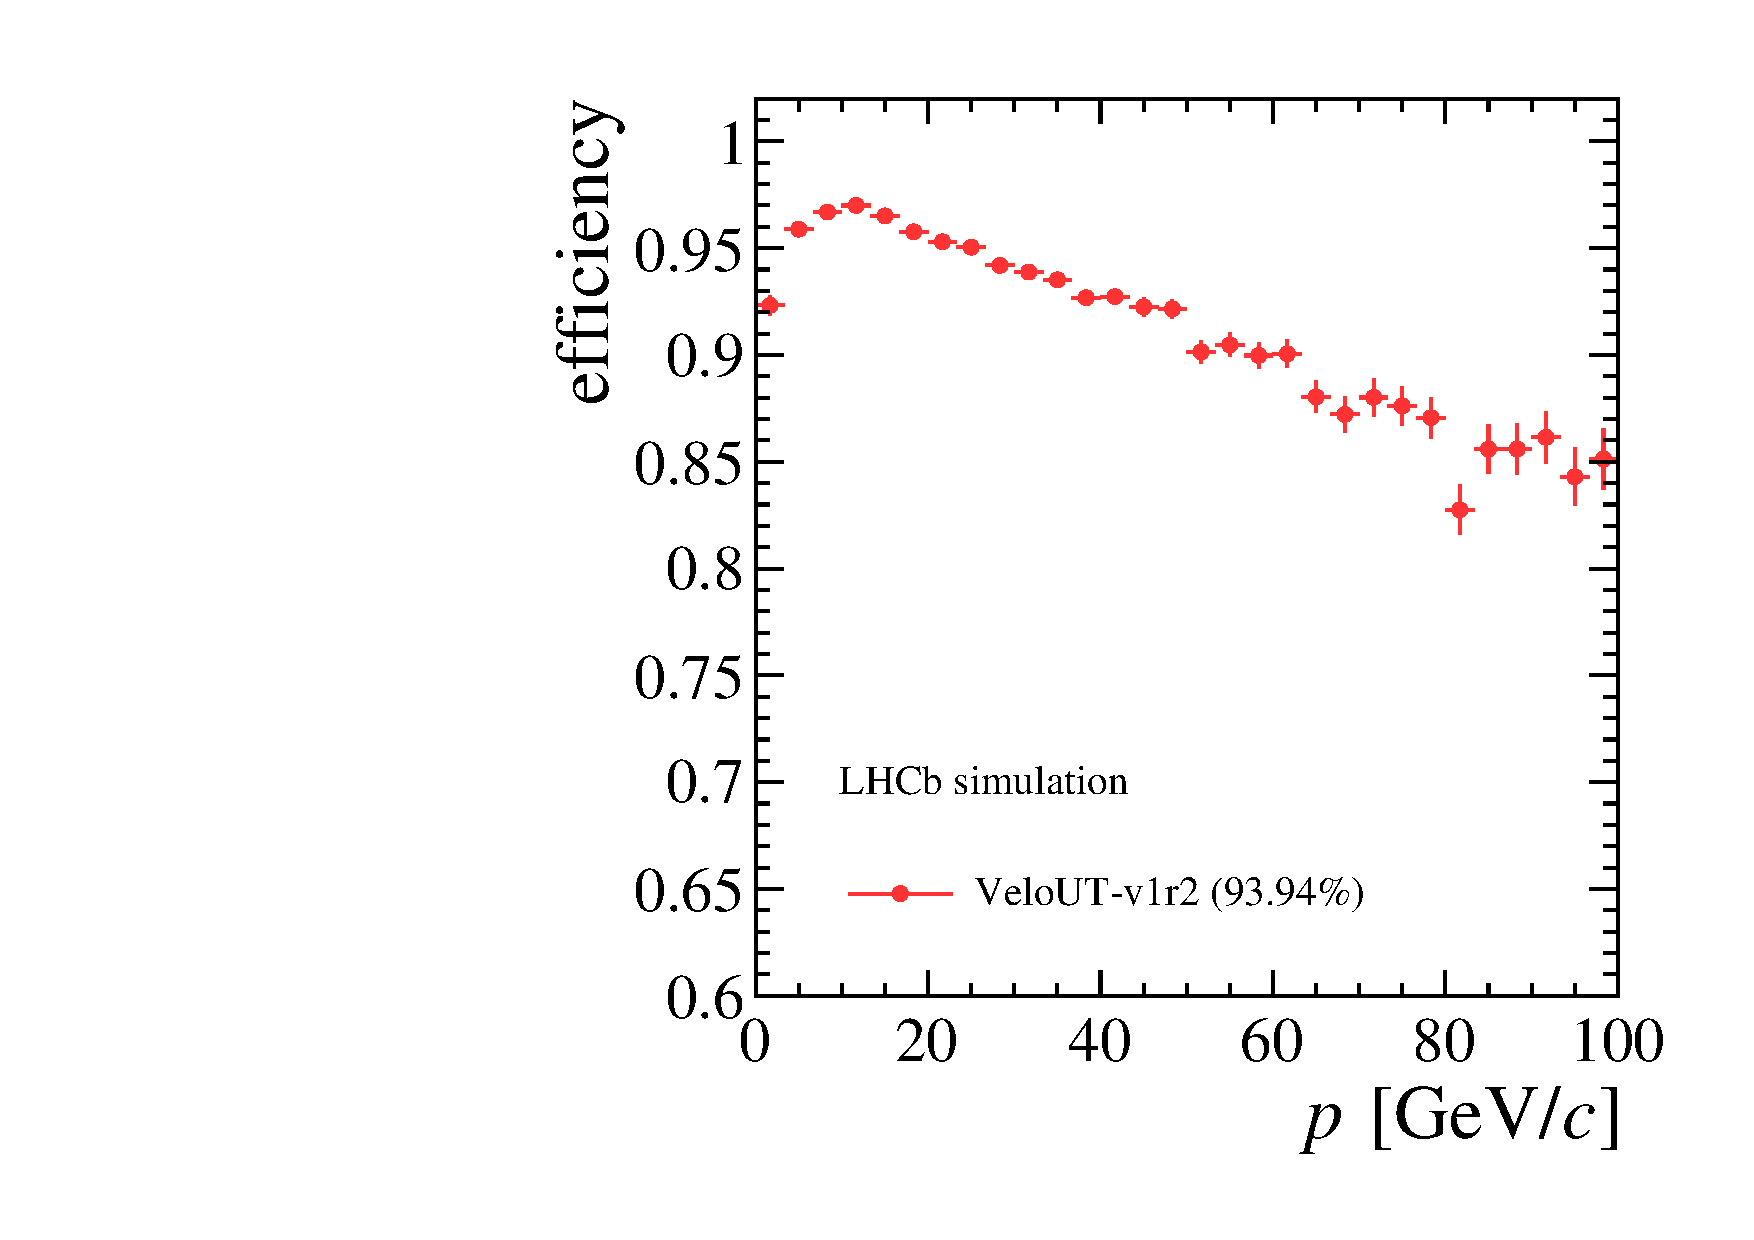
\includegraphics[width=0.45\textwidth]{figs/upstream-tracking-upgrade/eff_p_v1r2.pdf}
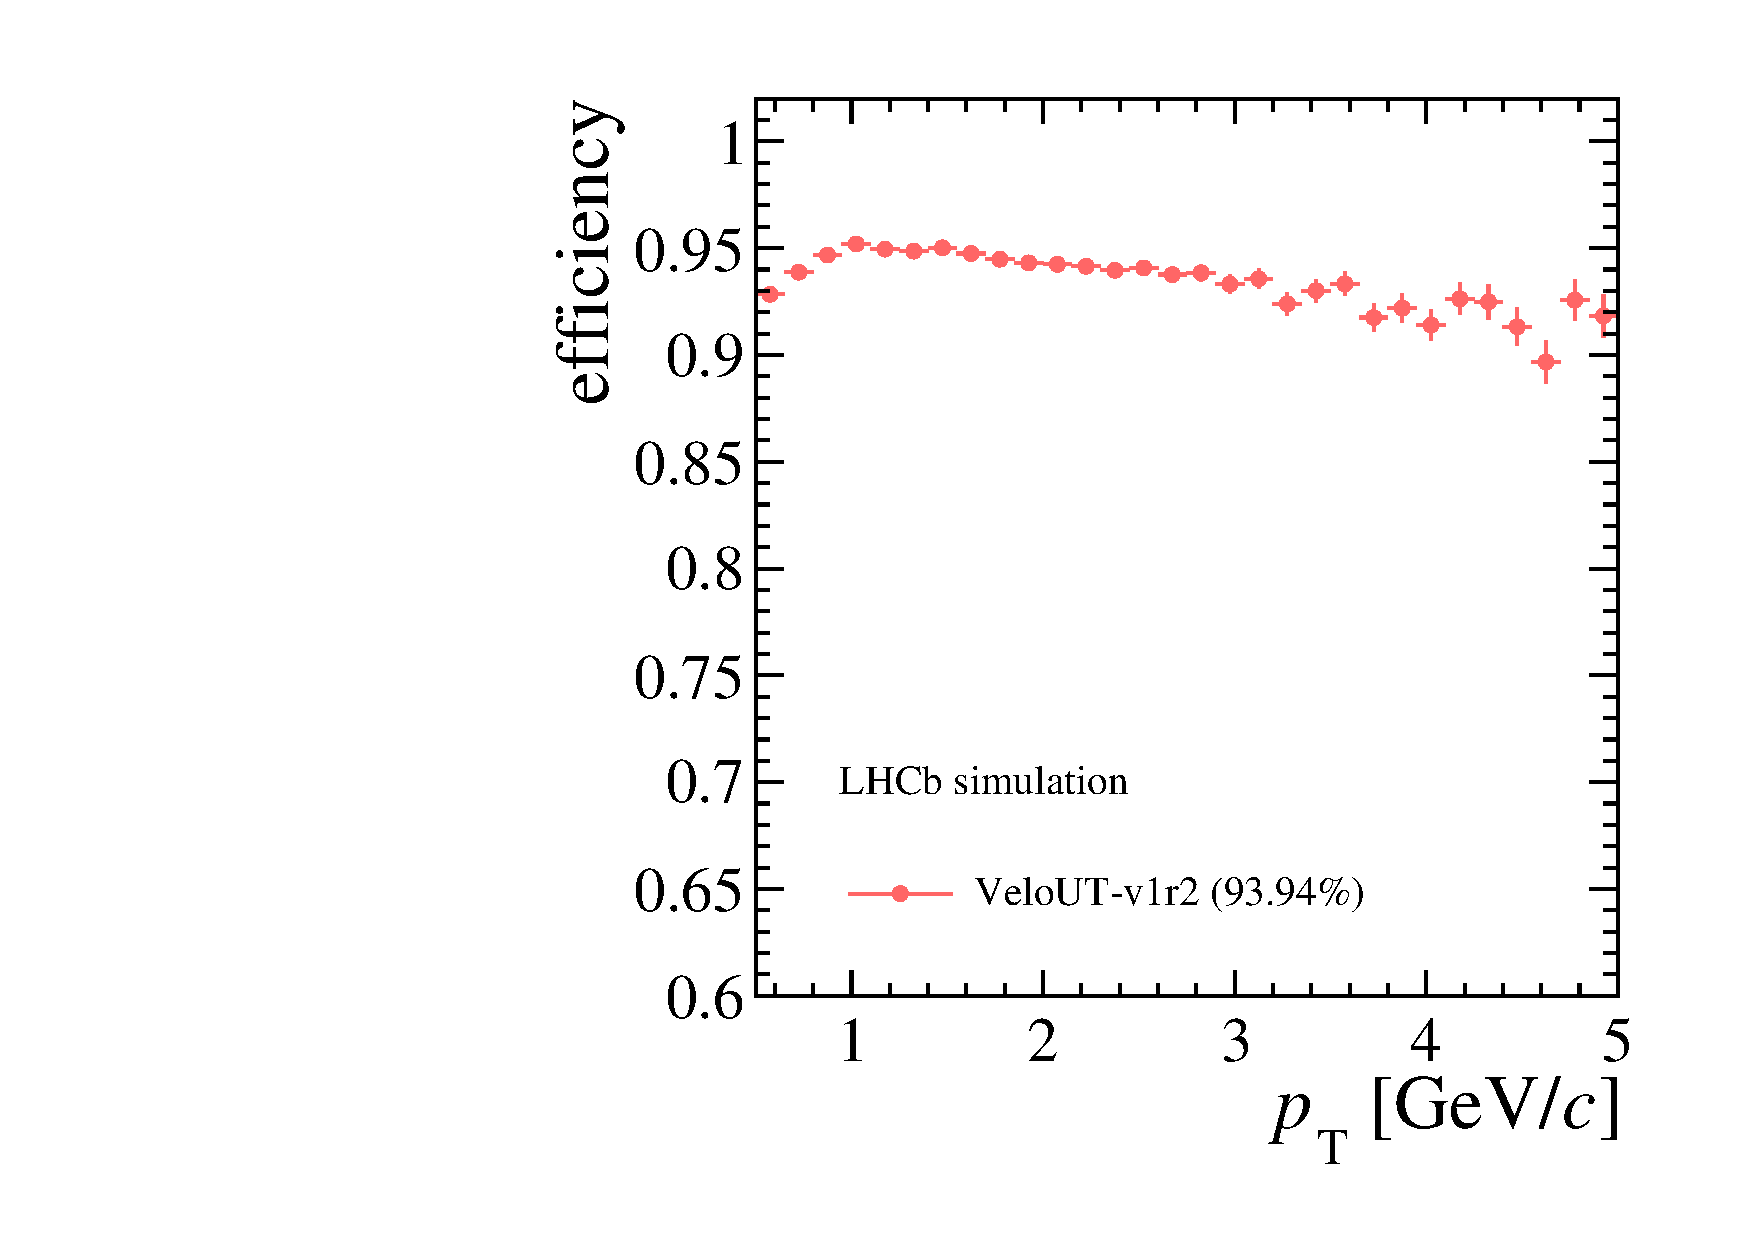
\includegraphics[width=0.45\textwidth]{figs/upstream-tracking-upgrade/eff_pt_v1r2.pdf}
\caption{The reconstruction efficiency as a function of \ptot and \pt for the initial version (\texttt{v1r2}) of the \velout algorithm. There is a clear drop in the reconstruction efficiency as a function of \ptot.}
\label{fig:eff_velout_v1r2}
\end{figure}

\begin{figure}[!tb]
\centering
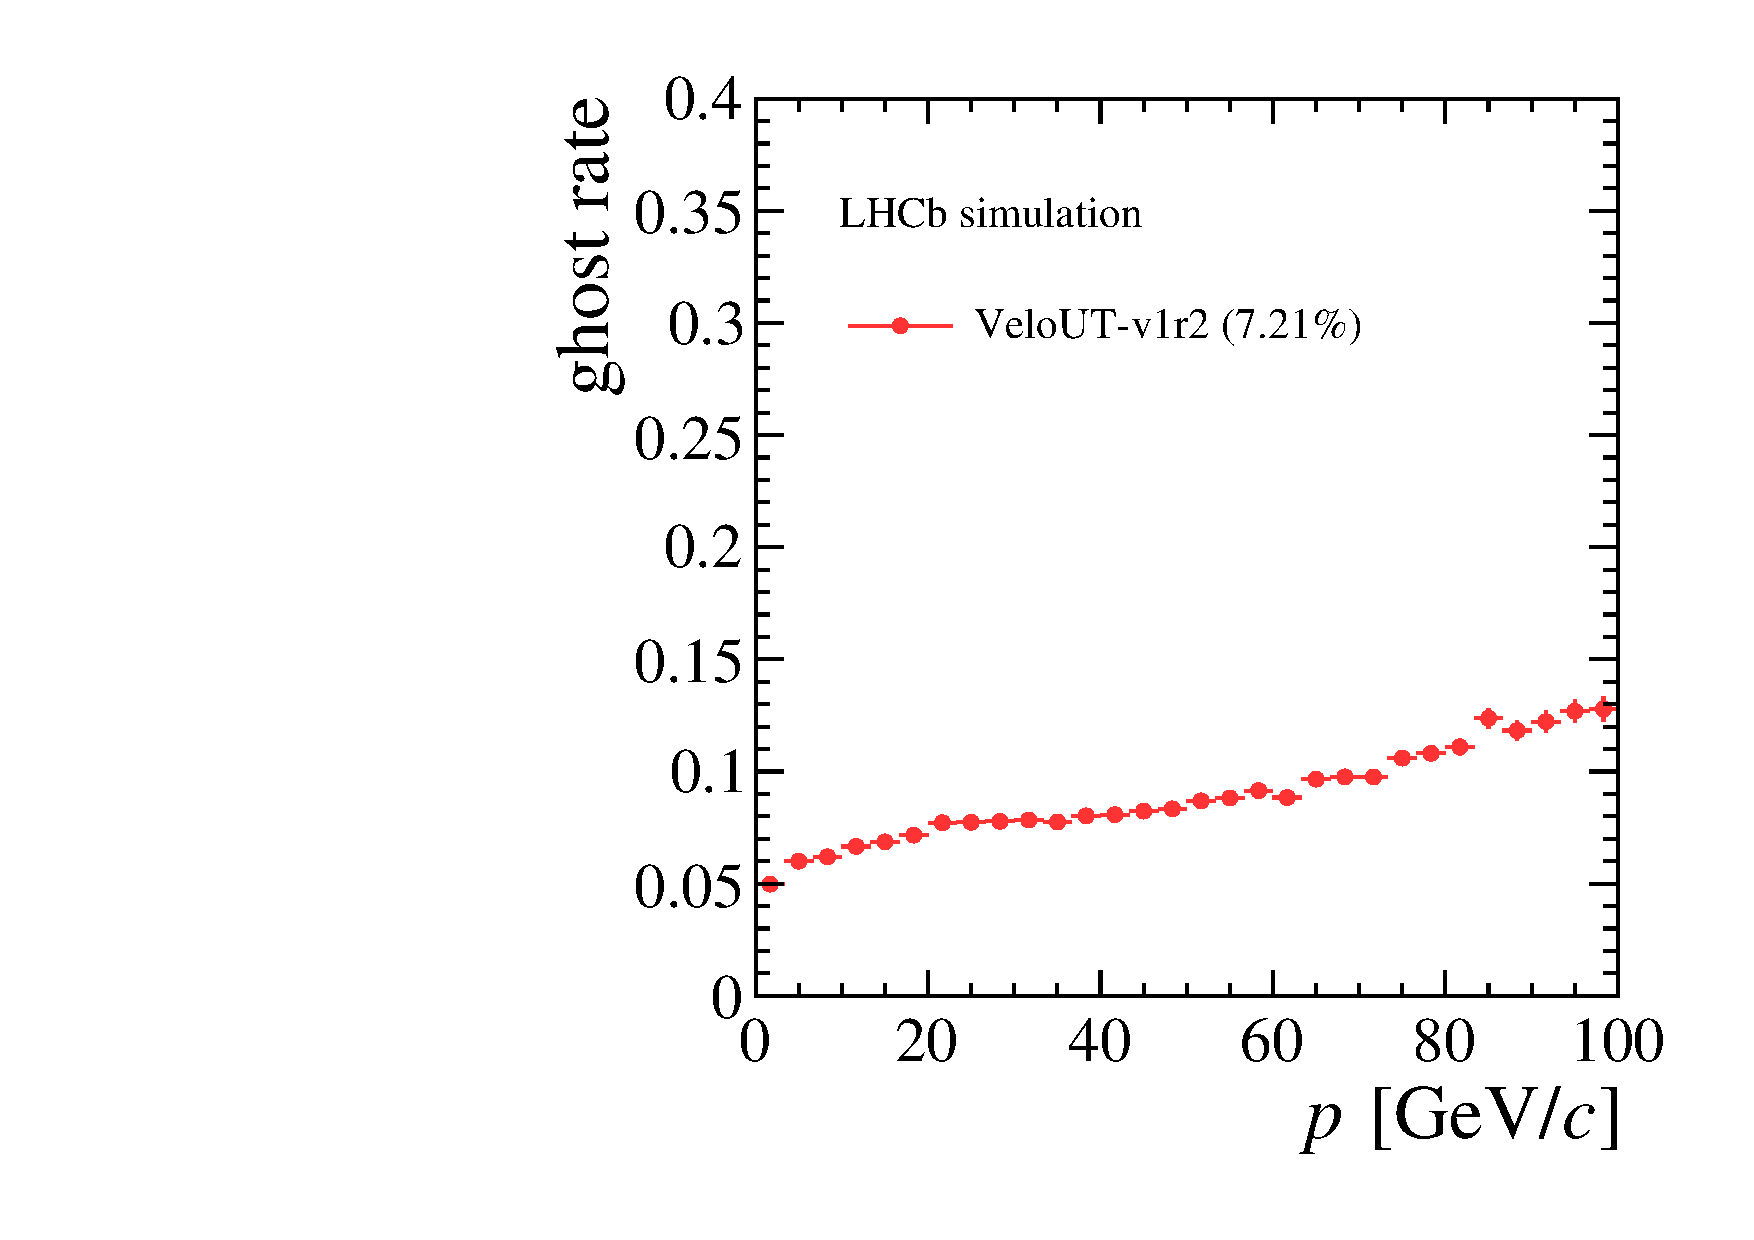
\includegraphics[width=0.45\textwidth]{figs/upstream-tracking-upgrade/gr_p_v1r2.pdf}
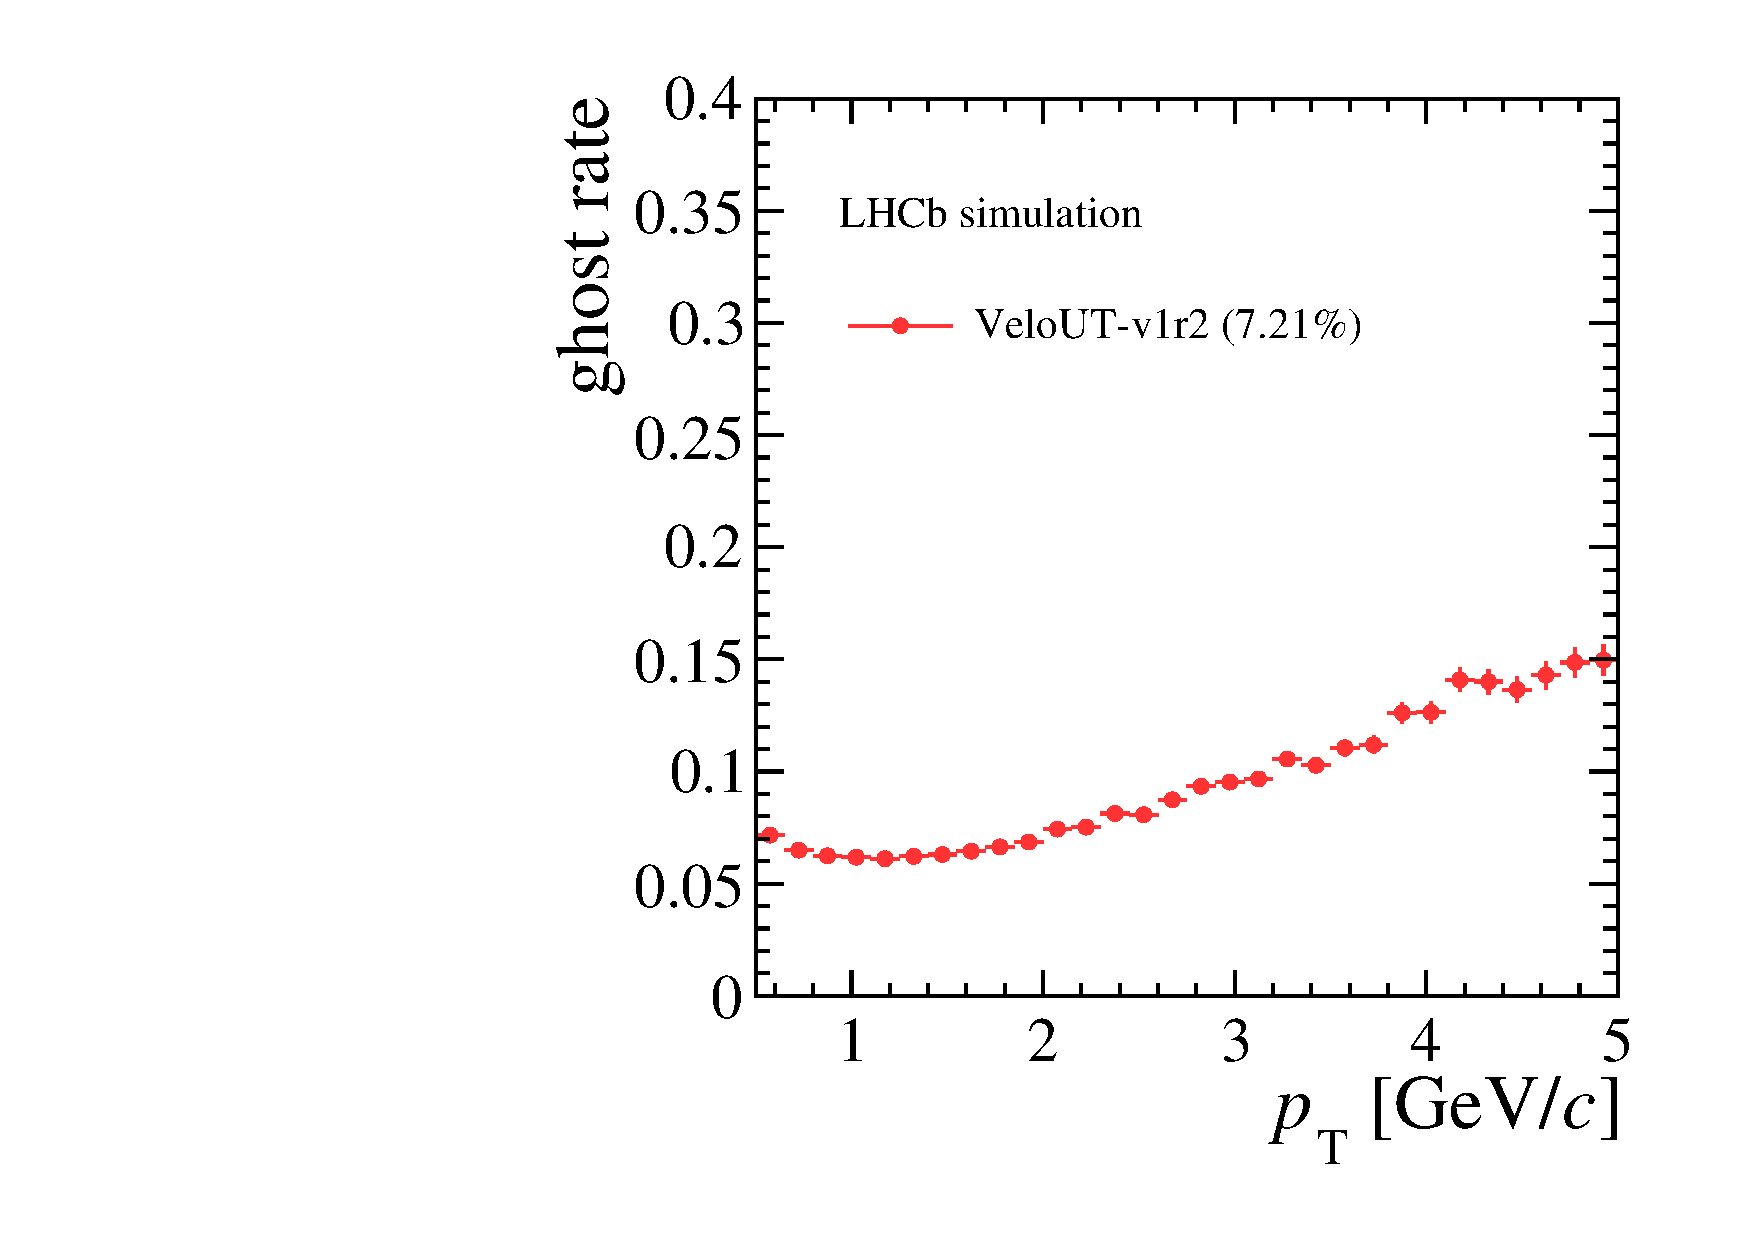
\includegraphics[width=0.45\textwidth]{figs/upstream-tracking-upgrade/gr_pt_v1r2.pdf}
\caption{The ghost rate as a function of \ptot and \pt for the initial version (\texttt{v1r2}) of the \velout algorithm.}
\label{fig:gr_velout_v1r2}
\end{figure}

\subsection{Improvements}

\subsubsection{Binary searches}

Previously, the hits were sorted by detector regions within layers. This meant that for each layer, each detector region was looped over and if it was compatible with the extrapolated \velo track each hit within that region was looped over. In the new version, the UT hits in each layer are sorted by their $x$ position at $y = 0$. For each layer, a binary search is performed to find the first hit which is within the search window. The hits are then looped over until that requirement is no longer satisfied. The new method greatly reduces the execution time.

\subsubsection{Clustering}

The inital version of the \velout algorithm used a Hough transform based on the distance of the hit from linear extrapolation of the \velo track to find cluster candidates. It required that all hits were located on one side of the extrapolated \velo track in the $x$-$z$ plane. While this is a good assumption for low \ptot tracks, it is not for high \ptot tracks as shown in Fig.~\ref{fig:wrong_side_hits}. This caused the track reconstruction efficiency to fall with increasing \ptot.

\begin{figure}[!tb]
\centering
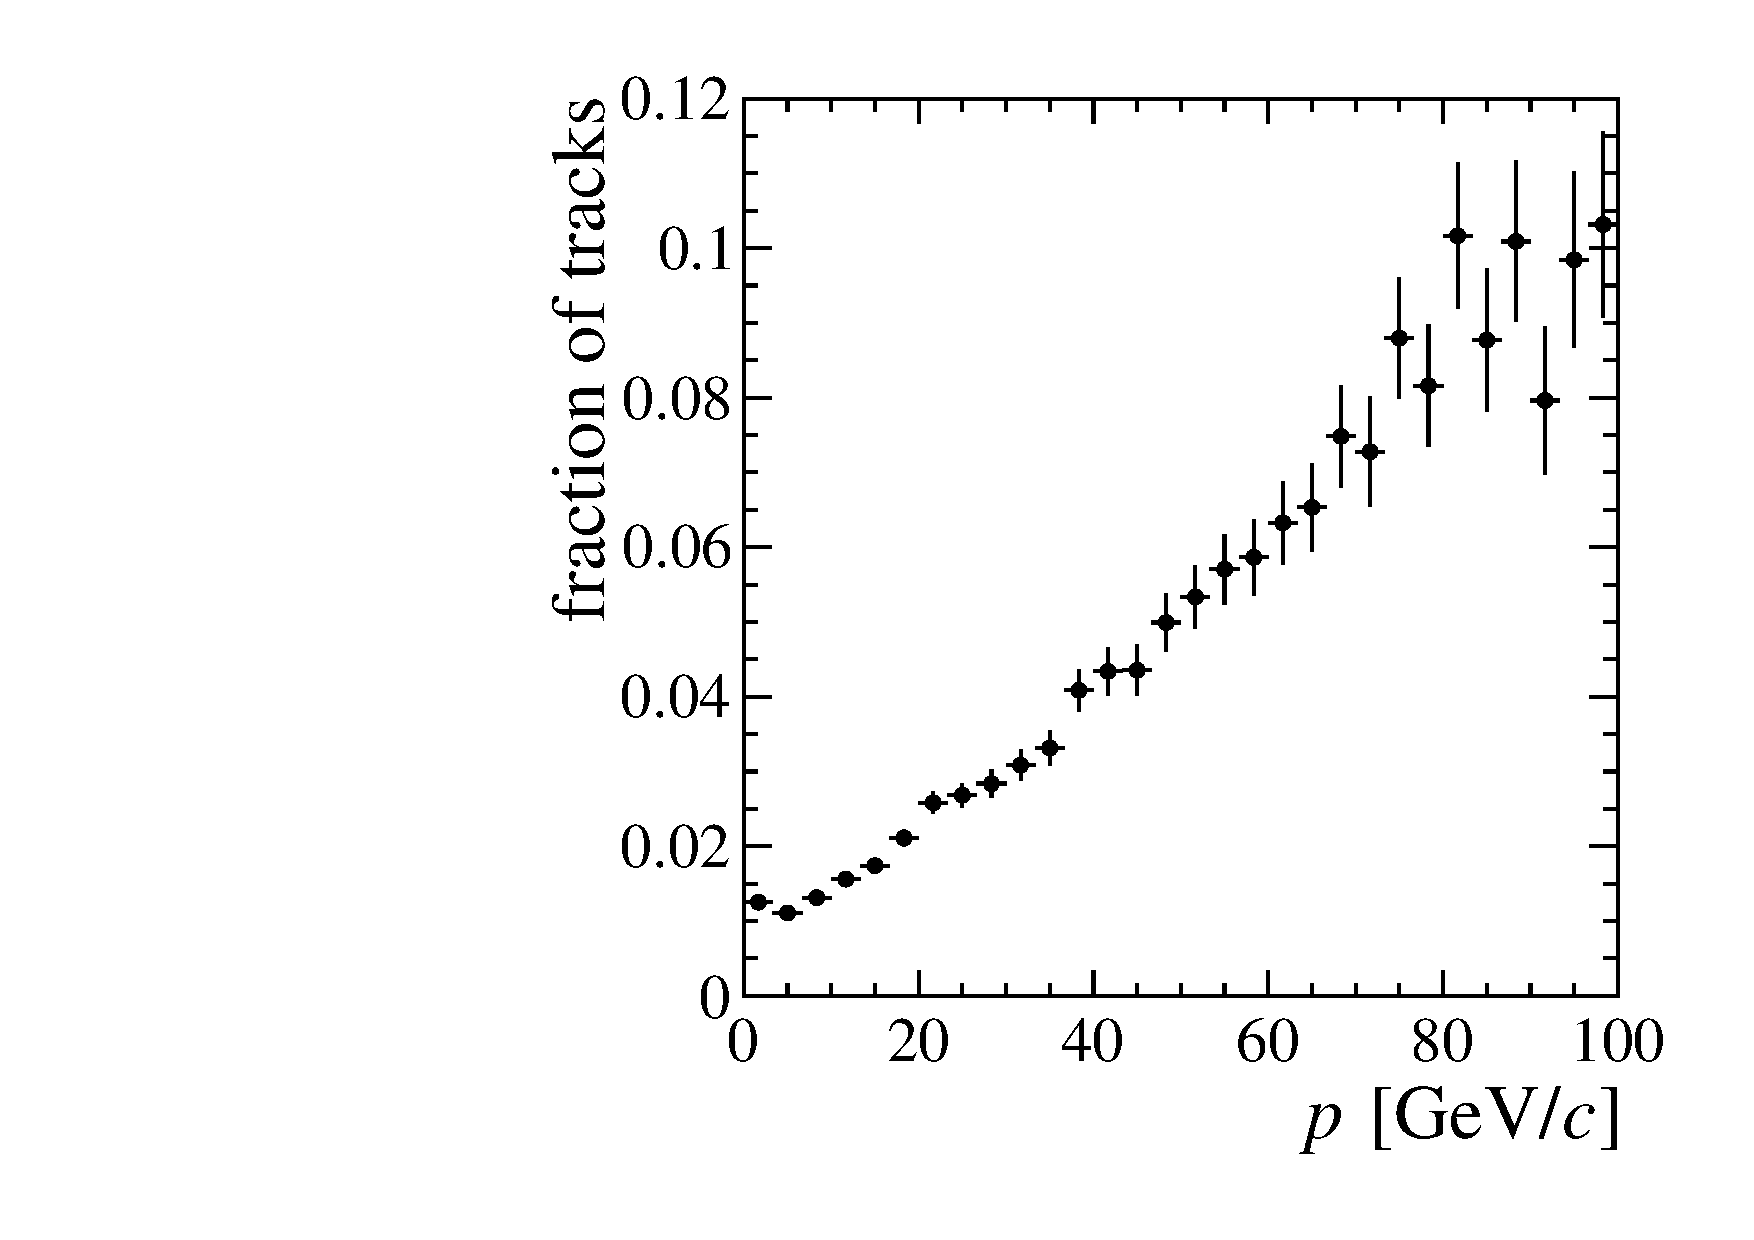
\includegraphics[width=0.45\textwidth]{figs/upstream-tracking-upgrade/wrong_side_hits.pdf}
\caption{The fraction of truth matched tracks with at least one hit on the opposite side of the linearly extrapolated \velo track in the $x$-$z$ plane.}% as a function of the true \ptot of the simulated particle.}
\label{fig:wrong_side_hits}
\end{figure}

The clustering of UT hits is shown schematically in Fig.~\ref{fig:clustering}. The hits are clustered by first forming doublets (two hits in the same station but in different layers), and then extending those doublets to the opposite station and searching for compatible hits to form triplets or quadruplets. 
 
A doublet is formed by taking one hit in the first layer and another in the second layer. The $x$-slope of the doublet is calculated and if it is below a given threshold the doublet is linearly extrapolated to the third layer where a tolerance window is opened. If there are compatible hits within this window, triplets are formed. For each triplet, the doublet is linearly extrapolated to the fourth layer. A reduced tolerance window is opened and compatible hits are used to form quadruplets. If no quadruplets are formed from any of the triplets, triplets are also searched for with the original doublet and hits in the fourth layer. This process is repeated for every doublet combination.
 
In order to account for missing hits in the UT detector, if no quadruplets have been formed the clustering sequence is run in reverse starting with a doublet in the third and fourth layers.
 
The tolerance window in $x$ around the extrapolated $x$ position of the doublet was tuned in simulation. Using simulated particles and their associated UT hits the difference, $\Delta x$, between the linearly extrapolated $x$ position of a doublet and the $x$ position of an associated hit in a given layer can be found. The distributions used for the tuning are shown in Fig.~\ref{fig:clustering_tolerance}.

\begin{figure}[!tb]
 \begin{center}
\resizebox{0.8\columnwidth}{!}{
  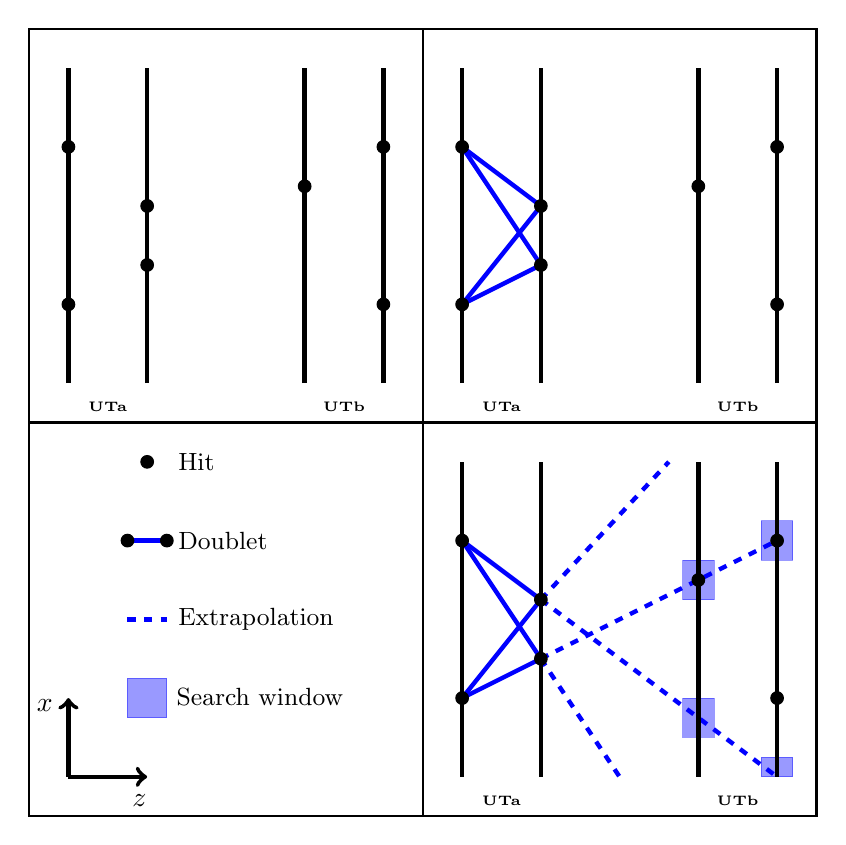
\begin{tikzpicture}
  %\draw[step=1cm,gray,very thin] (0,0) grid (10,10);

  %layout
  \draw[thick] (0,0) rectangle (5,5);
  \draw[thick] (5,0) rectangle (10,5);
  \draw[thick] (0,5) rectangle (5,10);
  \draw[thick] (5,5) rectangle (10,10);

  \draw[thick] (5.0,0.0) -- (5.0,10.0);
  \draw[thick] (0.0,5.0) -- (10.0,5.0);

  %first diagram
  %UT layers
  \draw[ultra thick] (0.5,5.5) -- (0.5,9.5);
  \draw[ultra thick] (1.5,5.5) -- (1.5,9.5);
  \draw[ultra thick] (3.5,5.5) -- (3.5,9.5);
  \draw[ultra thick] (4.5,5.5) -- (4.5,9.5);

  %true hits
  \draw[fill] (0.5,6.5) circle (0.08);
  \draw[fill] (1.5,7.0) circle (0.08);
  \draw[fill] (3.5,8.0) circle (0.08);
  \draw[fill] (4.5,8.5) circle (0.08);

  %fake hits
  \draw[fill] (0.5,8.5) circle (0.08);
  \draw[fill] (1.5,7.75) circle (0.08);
  \draw[fill] (4.5,6.5) circle (0.08);

  %labels
  \node[draw=none] at  (1,5.2){\tiny \bf{UTa}};
  \node[draw=none] at  (4,5.2){\tiny \bf{UTb}};

  %second diagram
  %doublets
  \draw[ultra thick,blue] (5.5,6.5) -- (6.5,7);
  \draw[ultra thick,blue] (5.5,6.5) -- (6.5,7.75);

  \draw[ultra thick,blue] (5.5,8.5) -- (6.5,7);
  \draw[ultra thick,blue] (5.5,8.5) -- (6.5,7.75);

  %UT layers
  \draw[ultra thick] (5.5,5.5) -- (5.5,9.5);
  \draw[ultra thick] (6.5,5.5) -- (6.5,9.5);
  \draw[ultra thick] (8.5,5.5) -- (8.5,9.5);
  \draw[ultra thick] (9.5,5.5) -- (9.5,9.5);

  %true hits
  \draw[fill] (5.5,6.5) circle (0.08);
  \draw[fill] (6.5,7.0) circle (0.08);
  \draw[fill] (8.5,8.0) circle (0.08);
  \draw[fill] (9.5,8.5) circle (0.08);

  %fake hits
  \draw[fill] (5.5,8.5) circle (0.08);
  \draw[fill] (6.5,7.75) circle (0.08);
  \draw[fill] (9.5,6.5) circle (0.08);

  %labels
  \node[draw=none] at  (6,5.2){\tiny \bf{UTa}};
  \node[draw=none] at  (9,5.2){\tiny \bf{UTb}};

  %third diagram
  %doublets
  \draw[ultra thick,blue] (5.5,1.5) -- (6.5,2.0);
  \draw[ultra thick,blue] (5.5,1.5) -- (6.5,2.75);

  \draw[ultra thick,blue] (5.5,3.5) -- (6.5,2.0);
  \draw[ultra thick,blue] (5.5,3.5) -- (6.5,2.75);

  %extrapolations
  %true
  \draw[ultra thick,blue,dashed] (6.5,2.0) -- (9.5,3.5);
  %fake
  \draw[ultra thick,blue,dashed] (6.5,2.0) -- (7.5,0.5);
  \draw[ultra thick,blue,dashed] (6.5,2.75) -- (8.125,4.5);
  \draw[ultra thick,blue,dashed] (6.5,2.75) -- (9.5,0.5);

  %search windows
  %true
  \draw[fill,blue,opacity=0.4] (8.3,2.75) rectangle (8.7,3.25);
  \draw[fill,blue,opacity=0.4] (9.3,3.25) rectangle (9.7,3.75);
  %fake
  \draw[fill,blue,opacity=0.4] (8.3,1.0) rectangle (8.7,1.50);
  \draw[fill,blue,opacity=0.4] (9.3,0.5) rectangle (9.7,0.75);

  %UT layers
  \draw[ultra thick] (5.5,0.5) -- (5.5,4.5);
  \draw[ultra thick] (6.5,0.5) -- (6.5,4.5);
  \draw[ultra thick] (8.5,0.5) -- (8.5,4.5);
  \draw[ultra thick] (9.5,0.5) -- (9.5,4.5);

  %true hits
  \draw[fill] (5.5,1.5) circle (0.08);
  \draw[fill] (6.5,2.0) circle (0.08);
  \draw[fill] (8.5,3.0) circle (0.08);
  \draw[fill] (9.5,3.5) circle (0.08);

  %fake hits
  \draw[fill] (5.5,3.5) circle (0.08);
  \draw[fill] (6.5,2.75) circle (0.08);
  \draw[fill] (9.5,1.5) circle (0.08);

  %labels
  \node[draw=none] at  (6,0.2){\tiny \bf{UTa}};
  \node[draw=none] at  (9,0.2){\tiny \bf{UTb}};

  %legend
  \draw[ultra thick, white] (1.25,4.5) -- (1.75,4.5)  node[anchor=west] {\small \textcolor{black}{Hit}};
  \draw[fill] (1.5,4.5) circle (0.08);

  \draw[ultra thick, blue] (1.25,3.5) -- (1.75,3.5)  node[anchor=west] {\small \textcolor{black}{Doublet}};
  \draw[fill] (1.25,3.5) circle (0.08);
  \draw[fill] (1.75,3.5) circle (0.08);

  \draw[ultra thick, blue,dashed] (1.25,2.5) -- (1.75,2.5) node[anchor=west] {\small \textcolor{black}{Extrapolation}};

  \draw[fill,blue,opacity=0.4,text opacity=1] (1.25,1.25) rectangle (1.75,1.75) node[anchor=north west] {\small \textcolor{black}{Search window}};

  \draw[ultra thick,->] (0.5,0.5) -- (0.5,1.5);
  \draw[ultra thick,->] (0.5,0.5) -- (1.5,0.5);
  \node[draw=none] at  (1.4,0.2){$z$};
  \node[draw=none] at  (0.2,1.4){$x$};

  \end{tikzpicture}
}
   
\caption{A schematic view of the clustering of UT hit candidates. Doublets in the first two layers are formed and then linearly extrapolated to the third and fourth layers to form triplets and quadruplets.}
\label{fig:clustering}
\end{center}
\end{figure}

\begin{figure}[!tb]
\centering
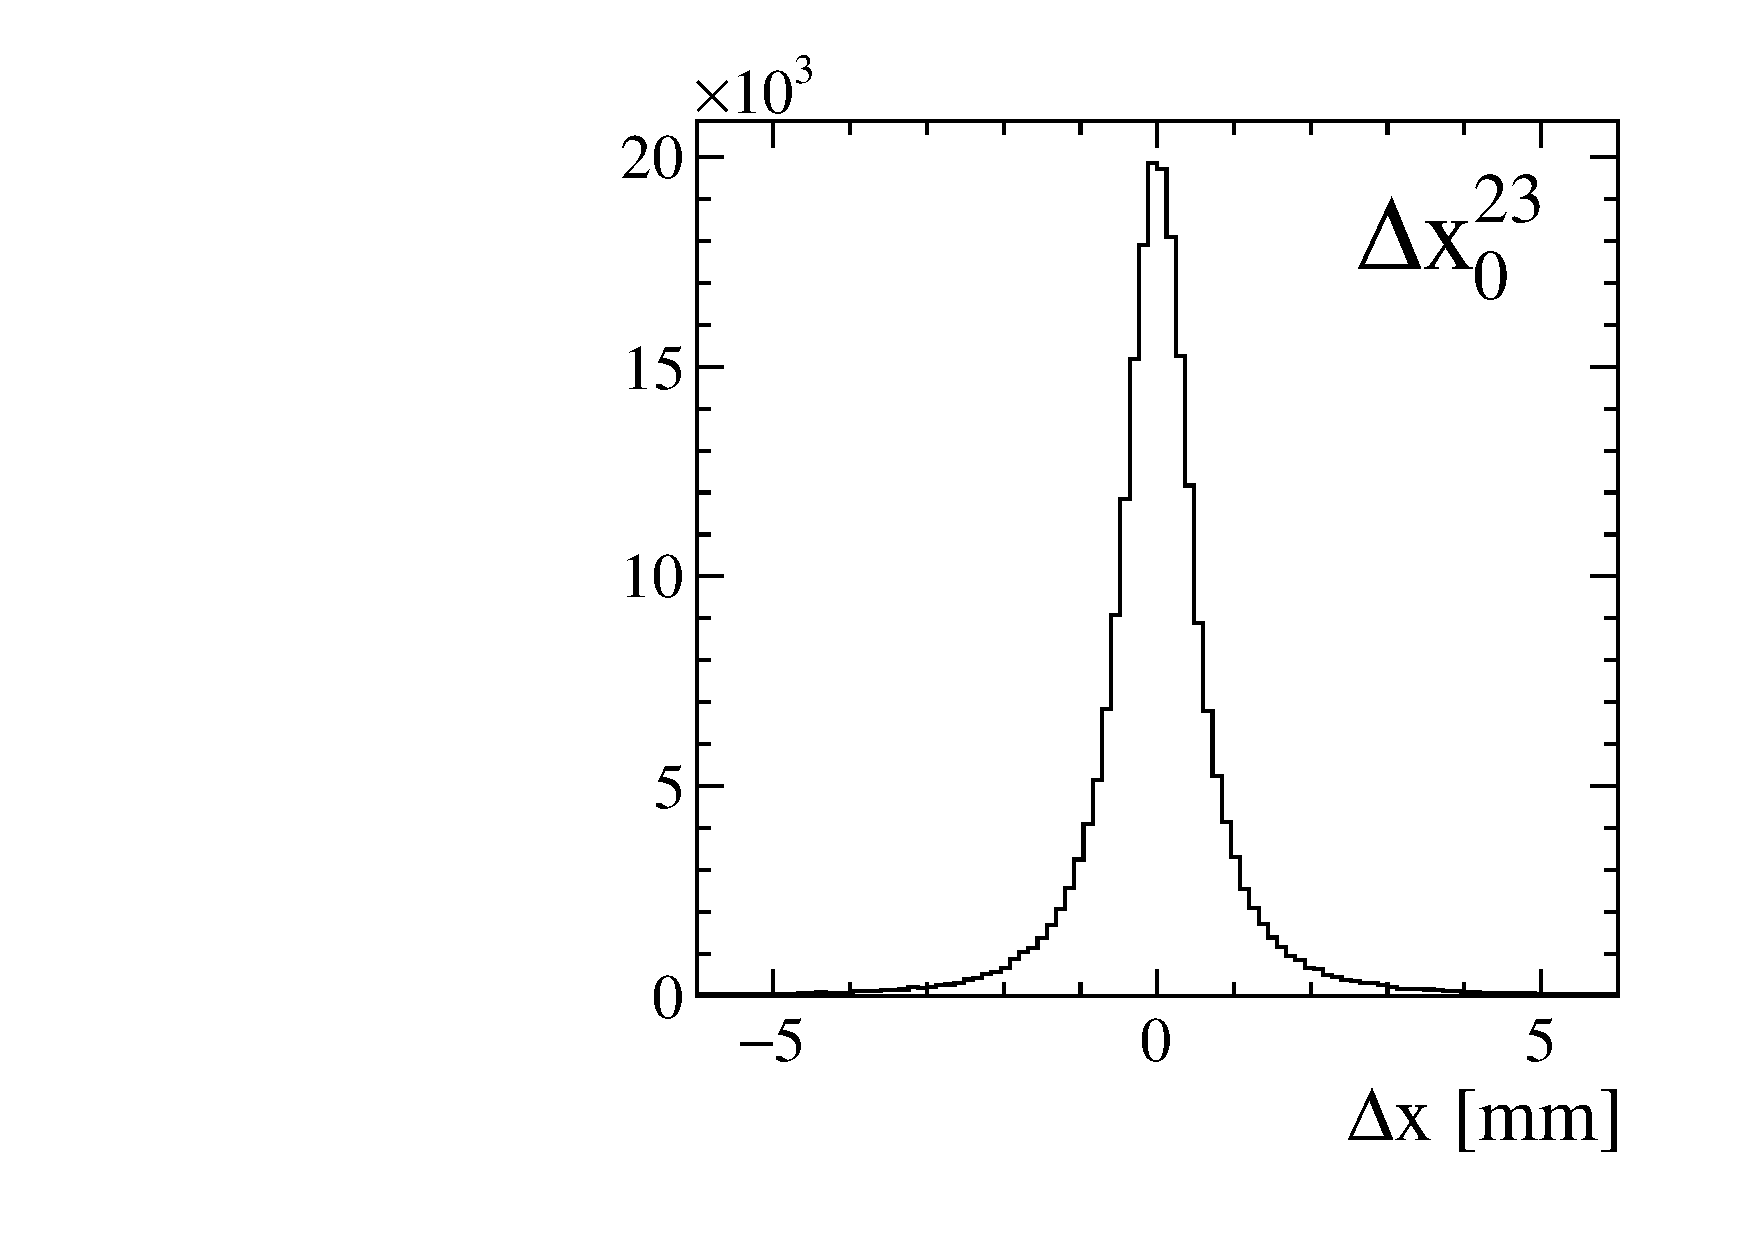
\includegraphics[width=0.32\textwidth]{figs/upstream-tracking-upgrade/dx0.pdf}
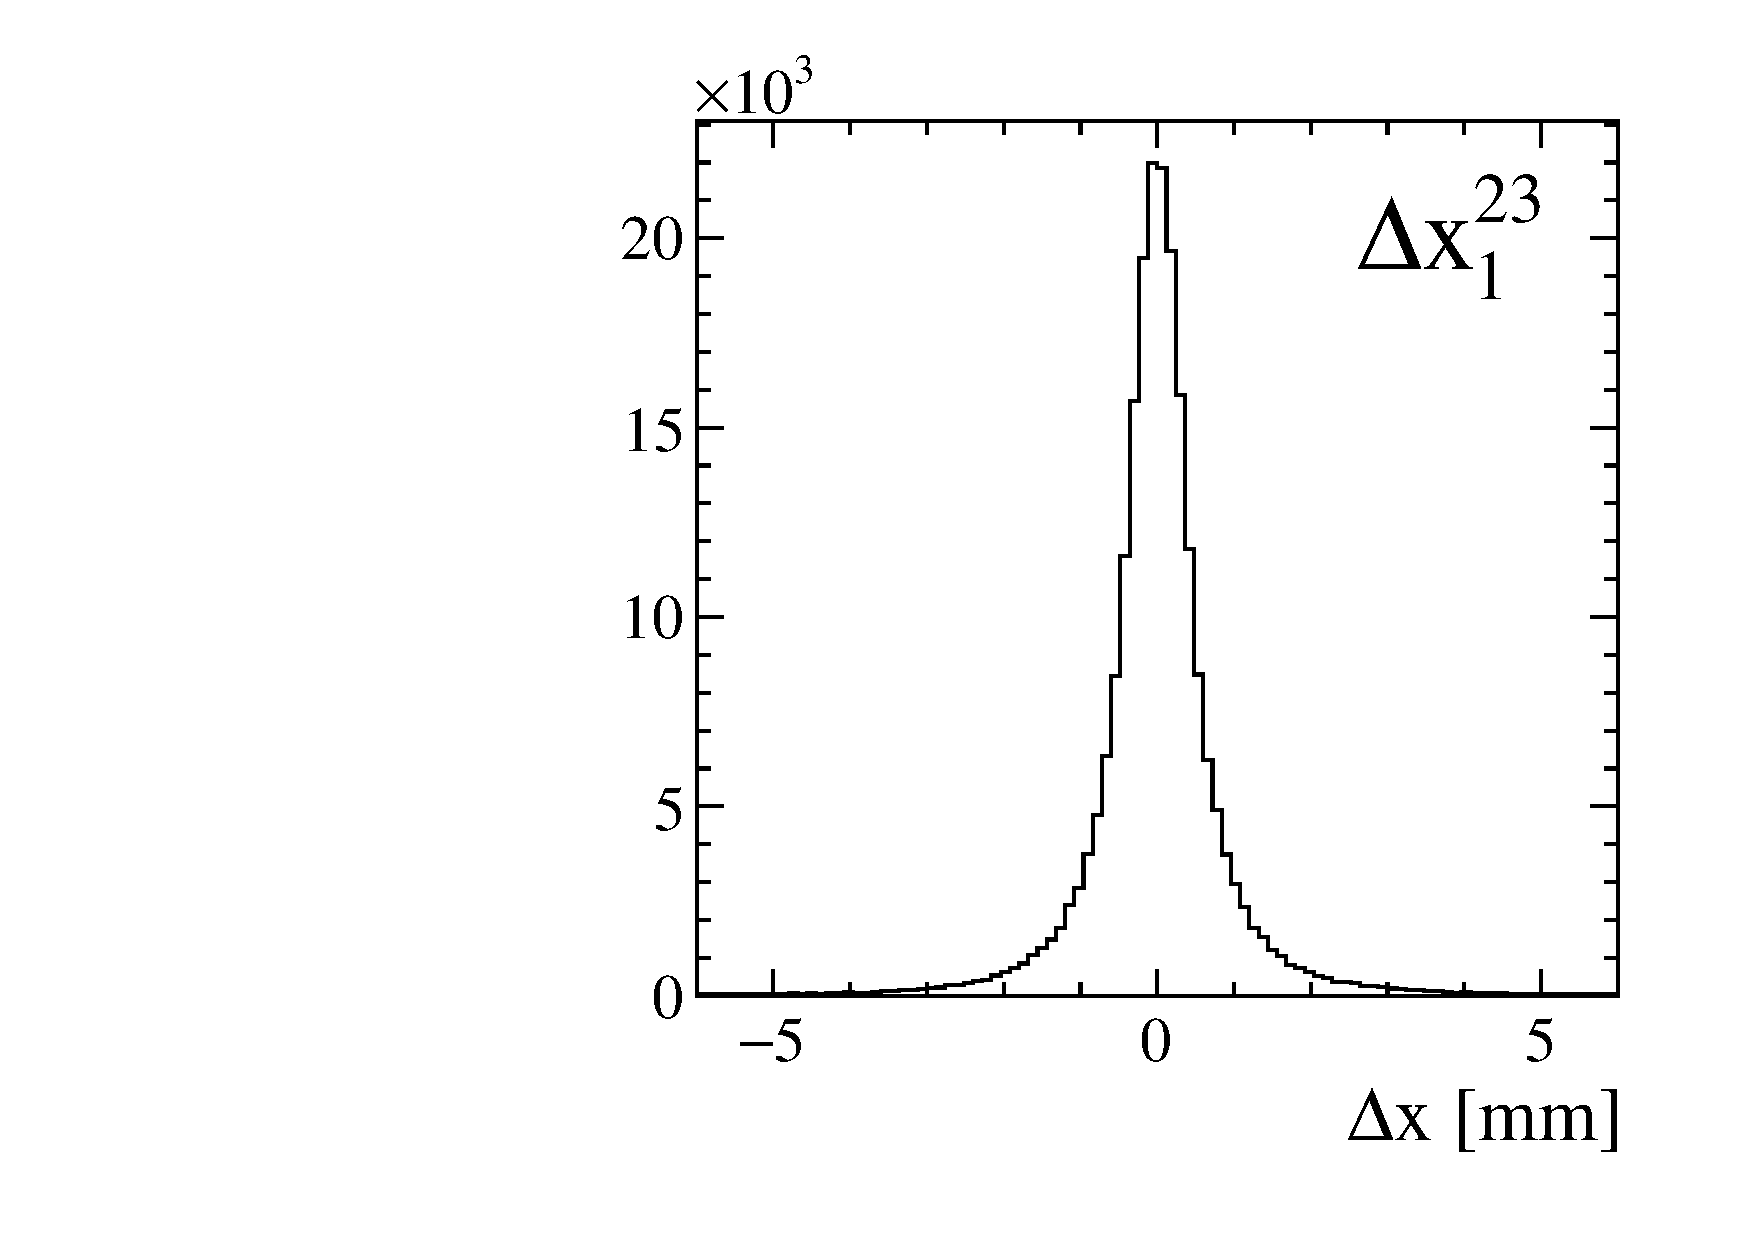
\includegraphics[width=0.32\textwidth]{figs/upstream-tracking-upgrade/dx1.pdf}
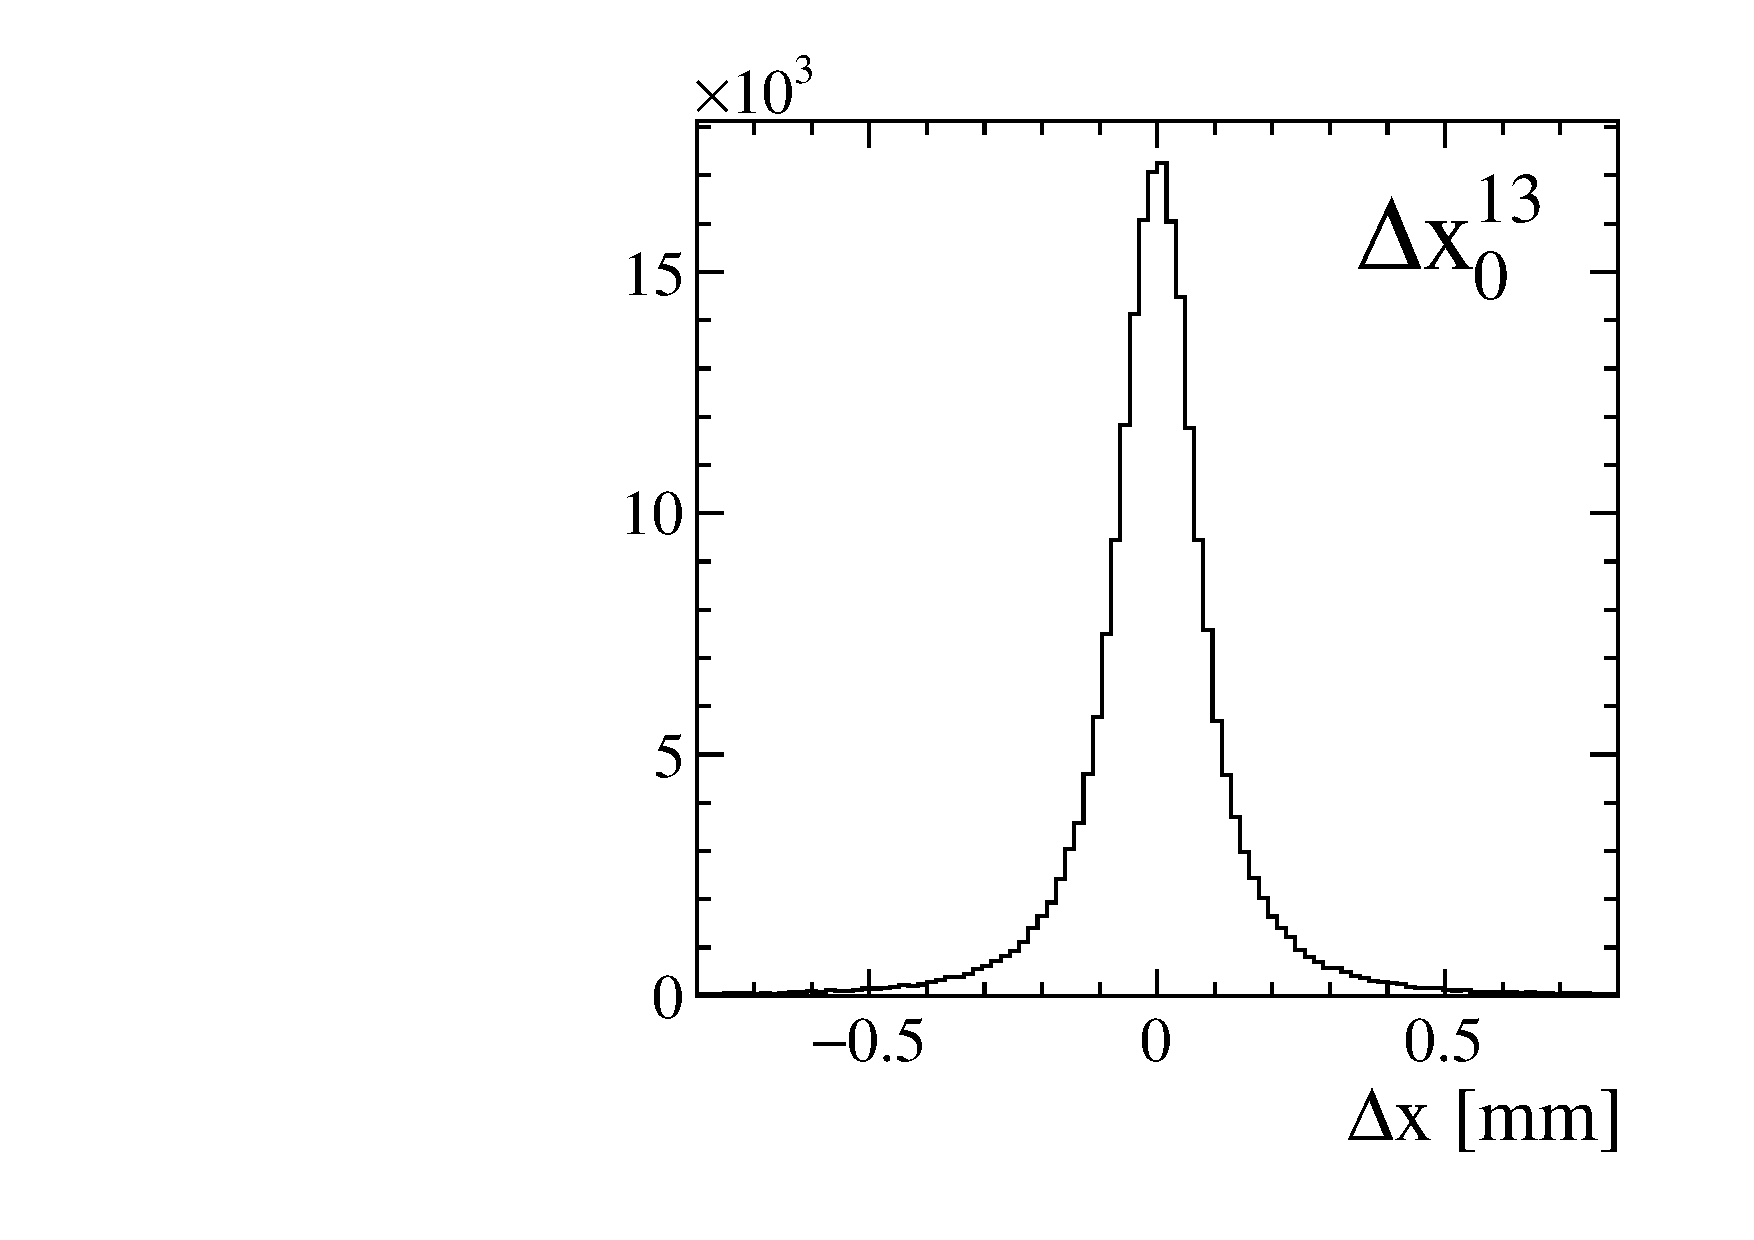
\includegraphics[width=0.32\textwidth]{figs/upstream-tracking-upgrade/dx0b.pdf}
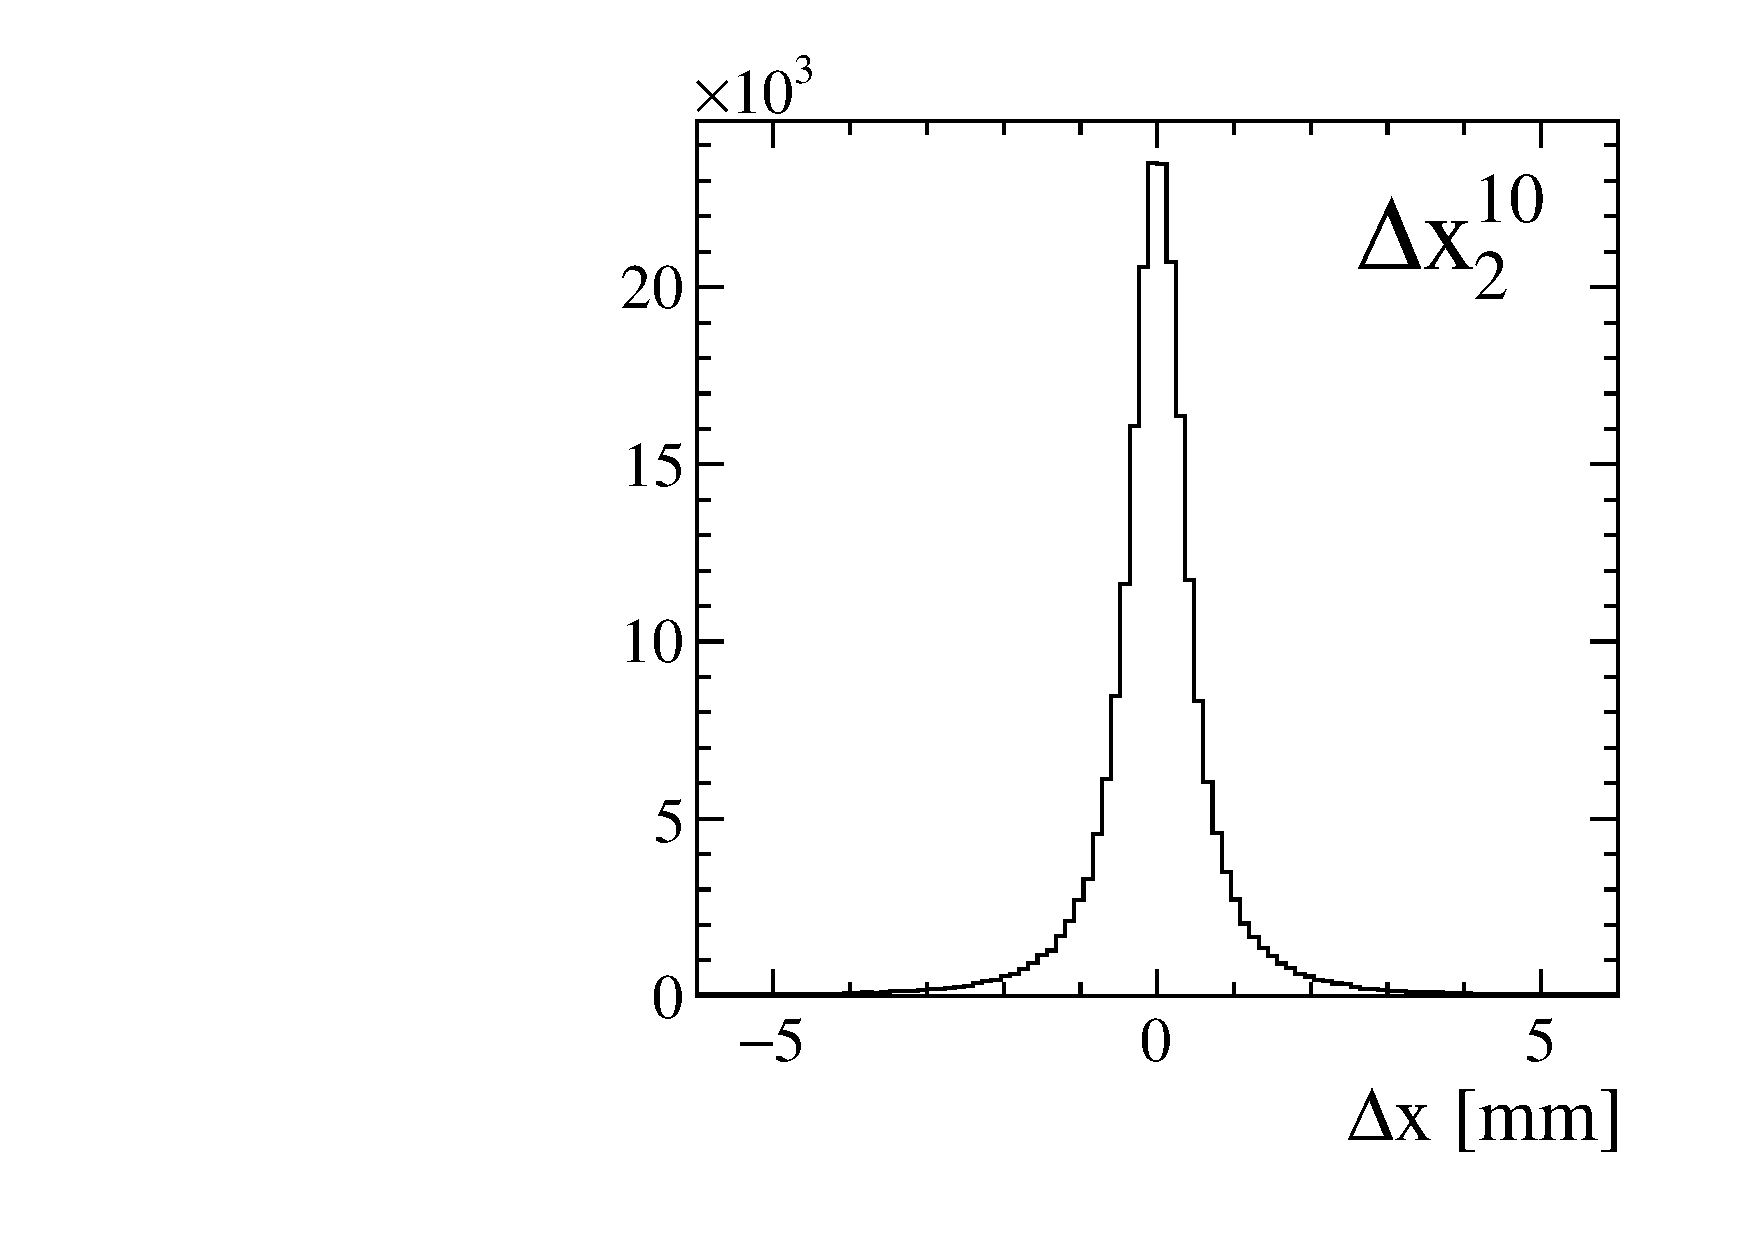
\includegraphics[width=0.32\textwidth]{figs/upstream-tracking-upgrade/dx2.pdf}
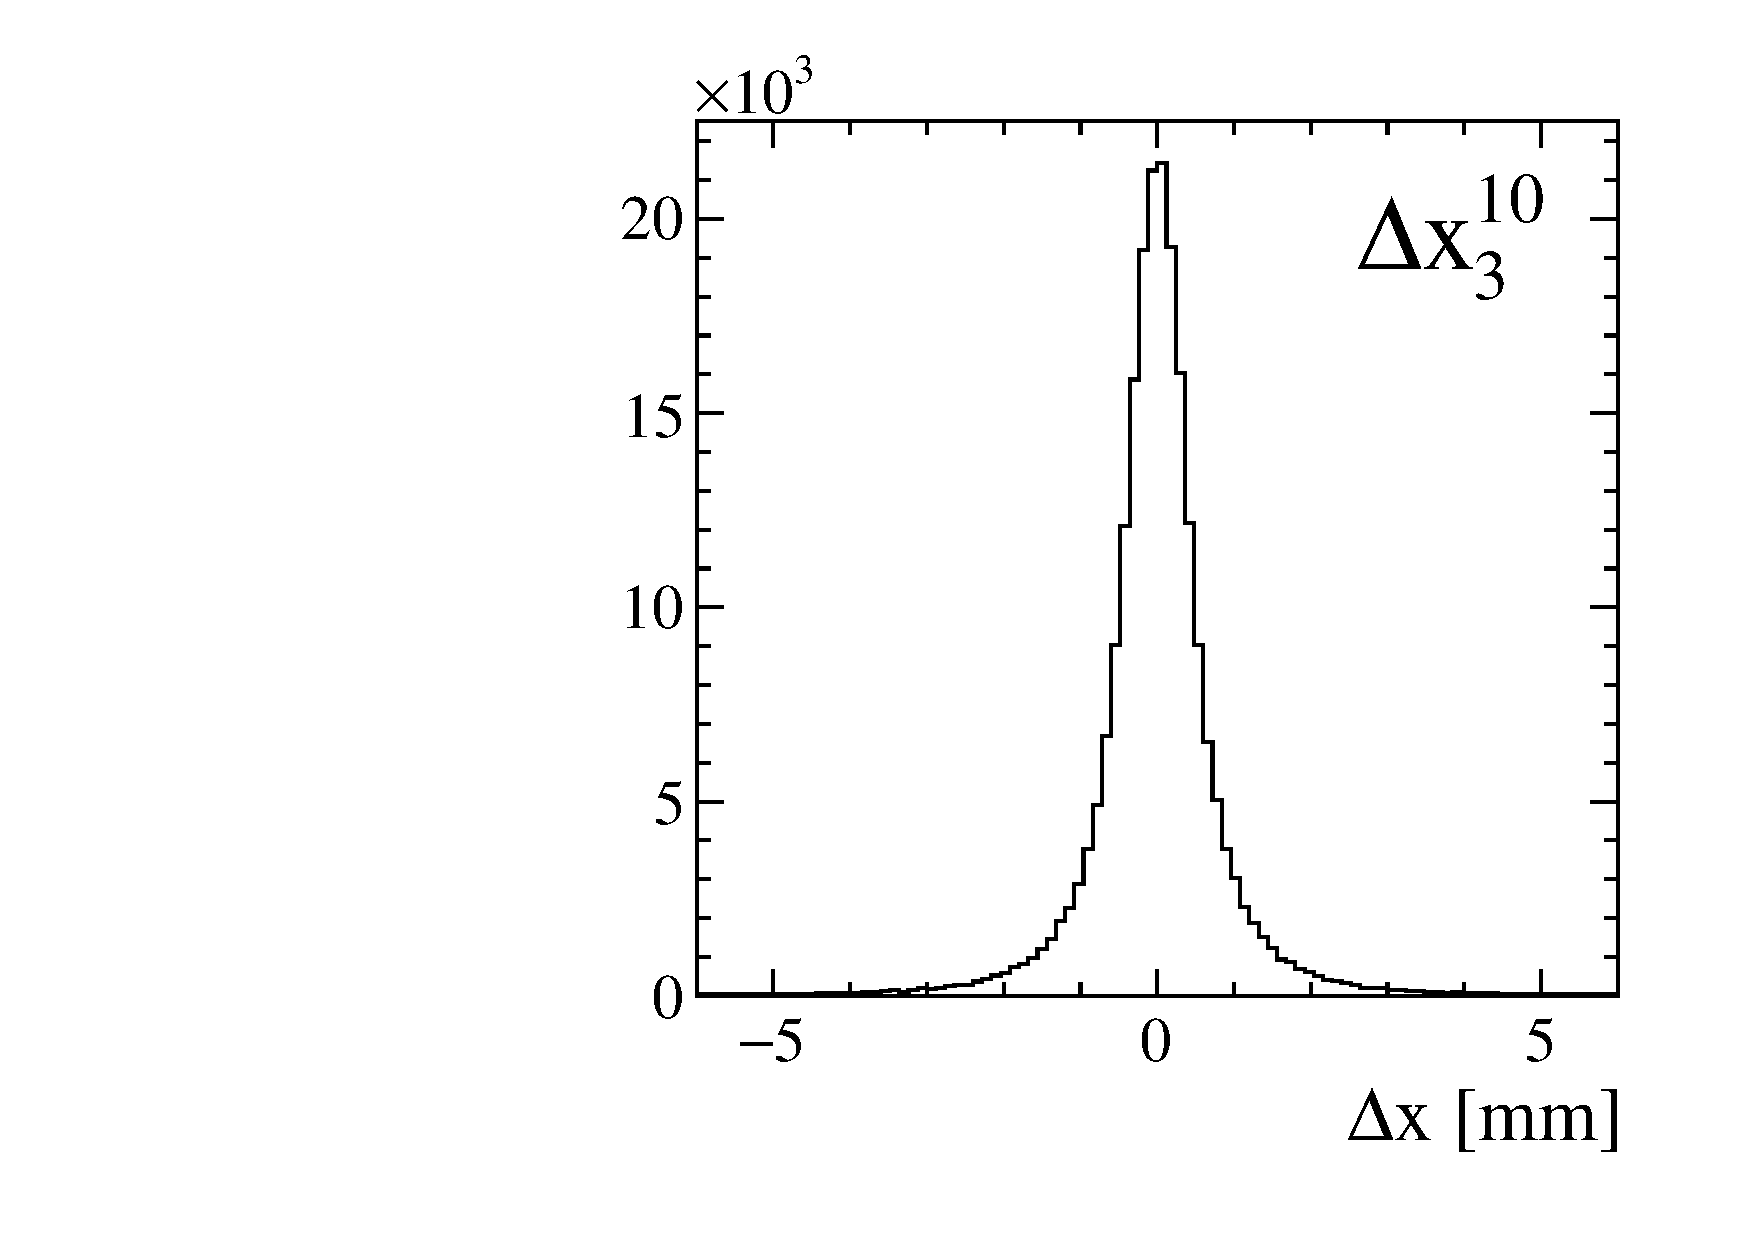
\includegraphics[width=0.32\textwidth]{figs/upstream-tracking-upgrade/dx3.pdf}
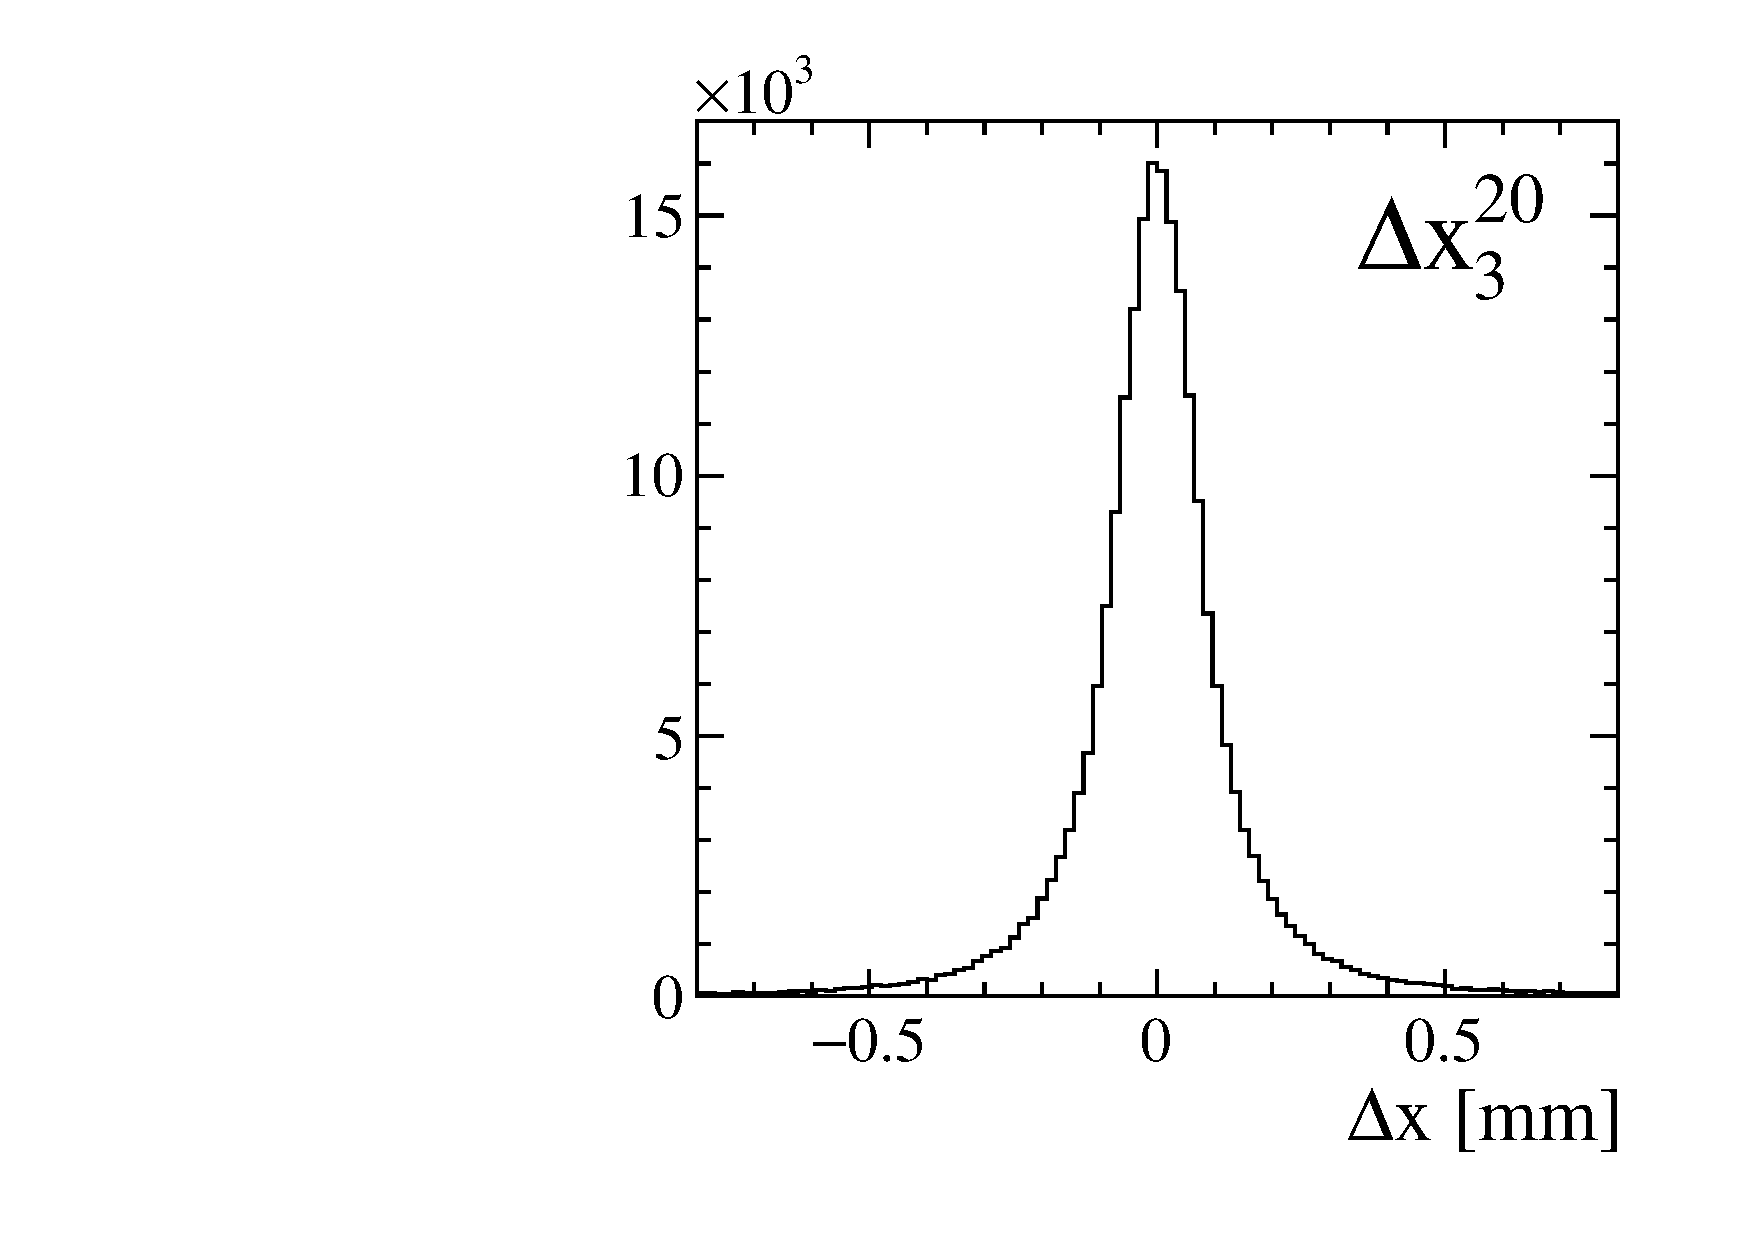
\includegraphics[width=0.32\textwidth]{figs/upstream-tracking-upgrade/dx3b.pdf}
\caption{The difference $\Delta x_{c}^{ab}$ between the linearly extrapolated $x$ position of a doublet and the $x$ position of an associated hit in a given layer where $a$ and $b$ denote the two layers from which the slope has been calculated and $c$ denotes the layer to which the extrapolation is being performed.}
\label{fig:clustering_tolerance}
\end{figure}


\subsubsection{Track fit}

The initial version fitted each of the \velout tracks with a Kalman filter, described in Sec.~\ref{sec:track:fit}, in order to the most accurate estimates of track parameters along with their corresponding covariances. This is very costly in terms of execution time and did not provided any significant improvement to the momentum or charge estimation. This fitting step was removed and the momentum and charge information taken from the simplified fit described in Sec.~\ref{sec:track:algos:upstream} leading to a vast improvement in the execution time.

\subsection{Upgrading to long tracks}

As described in Sec.~\ref{sec:up-track-upgrade:motivation}, \velout tracks rather than \velo tracks will be used input to the Forward tracking algorithm in the \lhcb Upgrade. Using the charge and momentum information of the \velout track it is possible to make smarter selections on the input tracks and T-station hits considered by the Forward algorithm. 

A preselection of \pt $>400$\mevc reduces the number of input tracks passed to the Forward tracking by a factor three compared to using \velo tracks. The charge information allows asymmetric search windows to be opened in the T-stations, reducing the hit multiplicity by a factor two. A small window is also opened on the `wrong' side of the linear extrapolation for high \pt candidates as they are more likely to have been assigned the incorrect charge. The optimised search windows are shown schematically in Fig.~\ref{fig:searchwindow}. These two advancements lead to a greatly reduced execution time and ghost rate of the Forward algorithm. In order to prevent inefficiency due to the central acceptance of UT, any \velo tracks that are linearly extrapolated within the central hole are passed directly to the Forward tracking algorithm.

\begin{figure}[!tb]
\resizebox{\columnwidth}{!}{
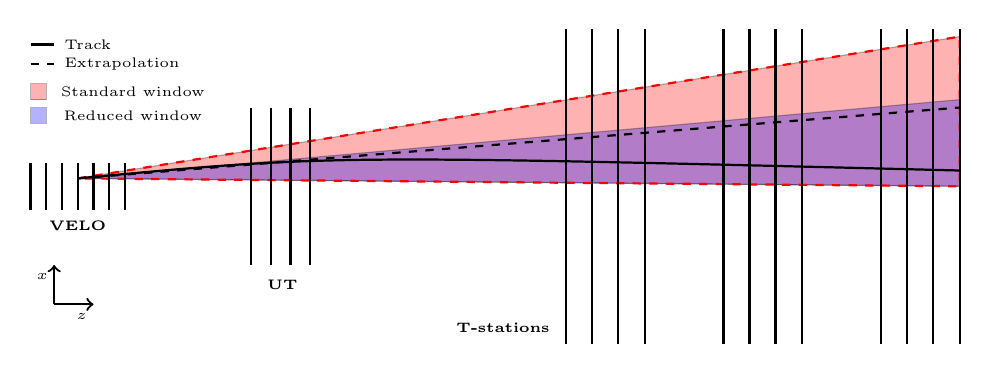
\begin{tikzpicture}
  %\draw[step=1cm,gray,very thin] (0,0) grid (12,4);

  \draw[fill=red,opacity=0.3] (0.8,2.1) -- (12.0,3.9) -- (12.0,2.0)--cycle;
  \draw[fill=blue,opacity=0.3] (0.8,2.1) -- (12.0,3.1) -- (12.0,2.0)--cycle;
  \draw[color=red,dashed,thick] (0.8,2.1) -- (12.0,3.9) -- (12.0,2.0)--cycle;

  %VELO
  \node[draw=none] at  (0.8,1.5){\tiny \bf{VELO}};
  \draw[thick] (0.2,1.7) -- (0.2,2.3);
  \draw[thick] (0.4,1.7) -- (0.4,2.3);
  \draw[thick] (0.6,1.7) -- (0.6,2.3);
  \draw[thick] (0.8,1.7) -- (0.8,2.3);
  \draw[thick] (1.0,1.7) -- (1.0,2.3);
  \draw[thick] (1.2,1.7) -- (1.2,2.3);
  \draw[thick] (1.4,1.7) -- (1.4,2.3);

  %TT
  \node[draw=none] at  (3.4,0.75){\tiny \bf{UT}};
  \draw[thick] (3.0,1.0) -- (3.0,3.0);
  \draw[thick] (3.25,1.0) -- (3.25,3.0);
  \draw[thick] (3.5,1.0) -- (3.5,3.0);
  \draw[thick] (3.75,1.0) -- (3.75,3.0);

  %T
  \node[draw=none] at  (6.2,0.2){\tiny \bf{T-stations}};
  \draw[thick] (7.0,0.0) -- (7.0,4.0);
  \draw[thick] (7.33,0.0) -- (7.33,4.0);
  \draw[thick] (7.66,0.0) -- (7.66,4.0);
  \draw[thick] (8.0,0.0) -- (8.0,4.0);

  \draw[thick] (9.0,0.0) -- (9.0,4.0);
  \draw[thick] (9.33,0.0) -- (9.33,4.0);
  \draw[thick] (9.66,0.0) -- (9.66,4.0);
  \draw[thick] (10.0,0.0) -- (10.0,4.0);

  \draw[thick] (11.0,0.0) -- (11.0,4.0);
  \draw[thick] (11.33,0.0) -- (11.33,4.0);
  \draw[thick] (11.66,0.0) -- (11.66,4.0);
  \draw[thick] (12.0,0.0) -- (12.0,4.0);

  \draw[thick,dashed] (0.8,2.1) -- (12,2+10*0.1);
  \draw[thick] (0.8,2.1) .. controls (4,2.4) .. (12,2.2);

  \draw[thick] (0.2,3.8) -- (0.5,3.8)  node[anchor=west] {\tiny Track};
  \draw[thick,dashed] (0.2,3.55) -- (0.5,3.55)  node[anchor=west] {\tiny Extrapolation};
  \draw[fill=red,opacity=0.3] (0.2,3.1) rectangle (0.4,3.3);
  \draw[fill=blue,opacity=0.3] (0.2,2.8) rectangle (0.4,3.0);

  \node[draw=none] at  (1.5,3.2){\tiny Standard window};
  \node[draw=none] at  (1.5,2.9){\tiny Reduced window};

  \draw[thick,->] (0.5,0.5) -- (0.5,1.0);
  \draw[thick,->] (0.5,0.5) -- (1.0,0.5);
  \node[draw=none] at (0.35,0.85){\tiny $x$};
  \node[draw=none] at (0.85,0.35){\tiny $z$};

\end{tikzpicture}
}

\caption{The search windows opened by the Forward algorithm with and without the charge and momentum information of the VeloUT candidates. The charge information allows asymmetric search windows to be opened. A small window is also opened on the `wrong' side of the linear extrapolation for high \pt candidates as they are more likely to have been assigned the incorrect charge.}
\label{fig:searchwindow}
\end{figure}

\subsection{Performance}

\subsubsection{\velout}

The track reconstruction efficiency, ghost rate and execution time of the \velout algorithm for both the initial version (\texttt{v1r2}) and the optimised version (\texttt{v2r2}) are shown in Tab.~\ref{tab:perf_velout_comp}. The track reconstruction efficiency as a function of \ptot and \pt are shown in Fig.~\ref{fig:eff_velout_comp}. The ghost rate as a function of \ptot and \pt are shown in Fig.~\ref{fig:gr_velout_comp}. The optimised version shows large improvements in terms of track reconstruction efficiency and execution time. The increase in reconstruction efficiency is most evident at high \ptot where the initial version shows a negative trend for increasing \ptot. There is also a slight increase in the ghost rate. However, this is of lesser importance as the ghost rate can be further reduced during offline analysis.

\begin{table}[!tb]
\caption{The performances of both the initial version (\texttt{v1r2}) and the optimised version (\texttt{v2r2}) of the \velout algorithm in terms of track reconstruction efficiency, ghost rate and execution time.}
\begin{center}
\begin{tabular}{c|c|c|c}
   \velout & Efficiency [\%] & Ghost rate [\%] & Timing [ms] \\
   \hline
   v1r2  & 93.94  & 7.21  &  27.20  \\
   v2r2  & 98.69  & 8.00 &  \hphantom{0}0.81  \\
 \end{tabular}
 \end{center}
\label{tab:perf_velout_comp}
\end{table}

\begin{figure}[!tb]
\centering
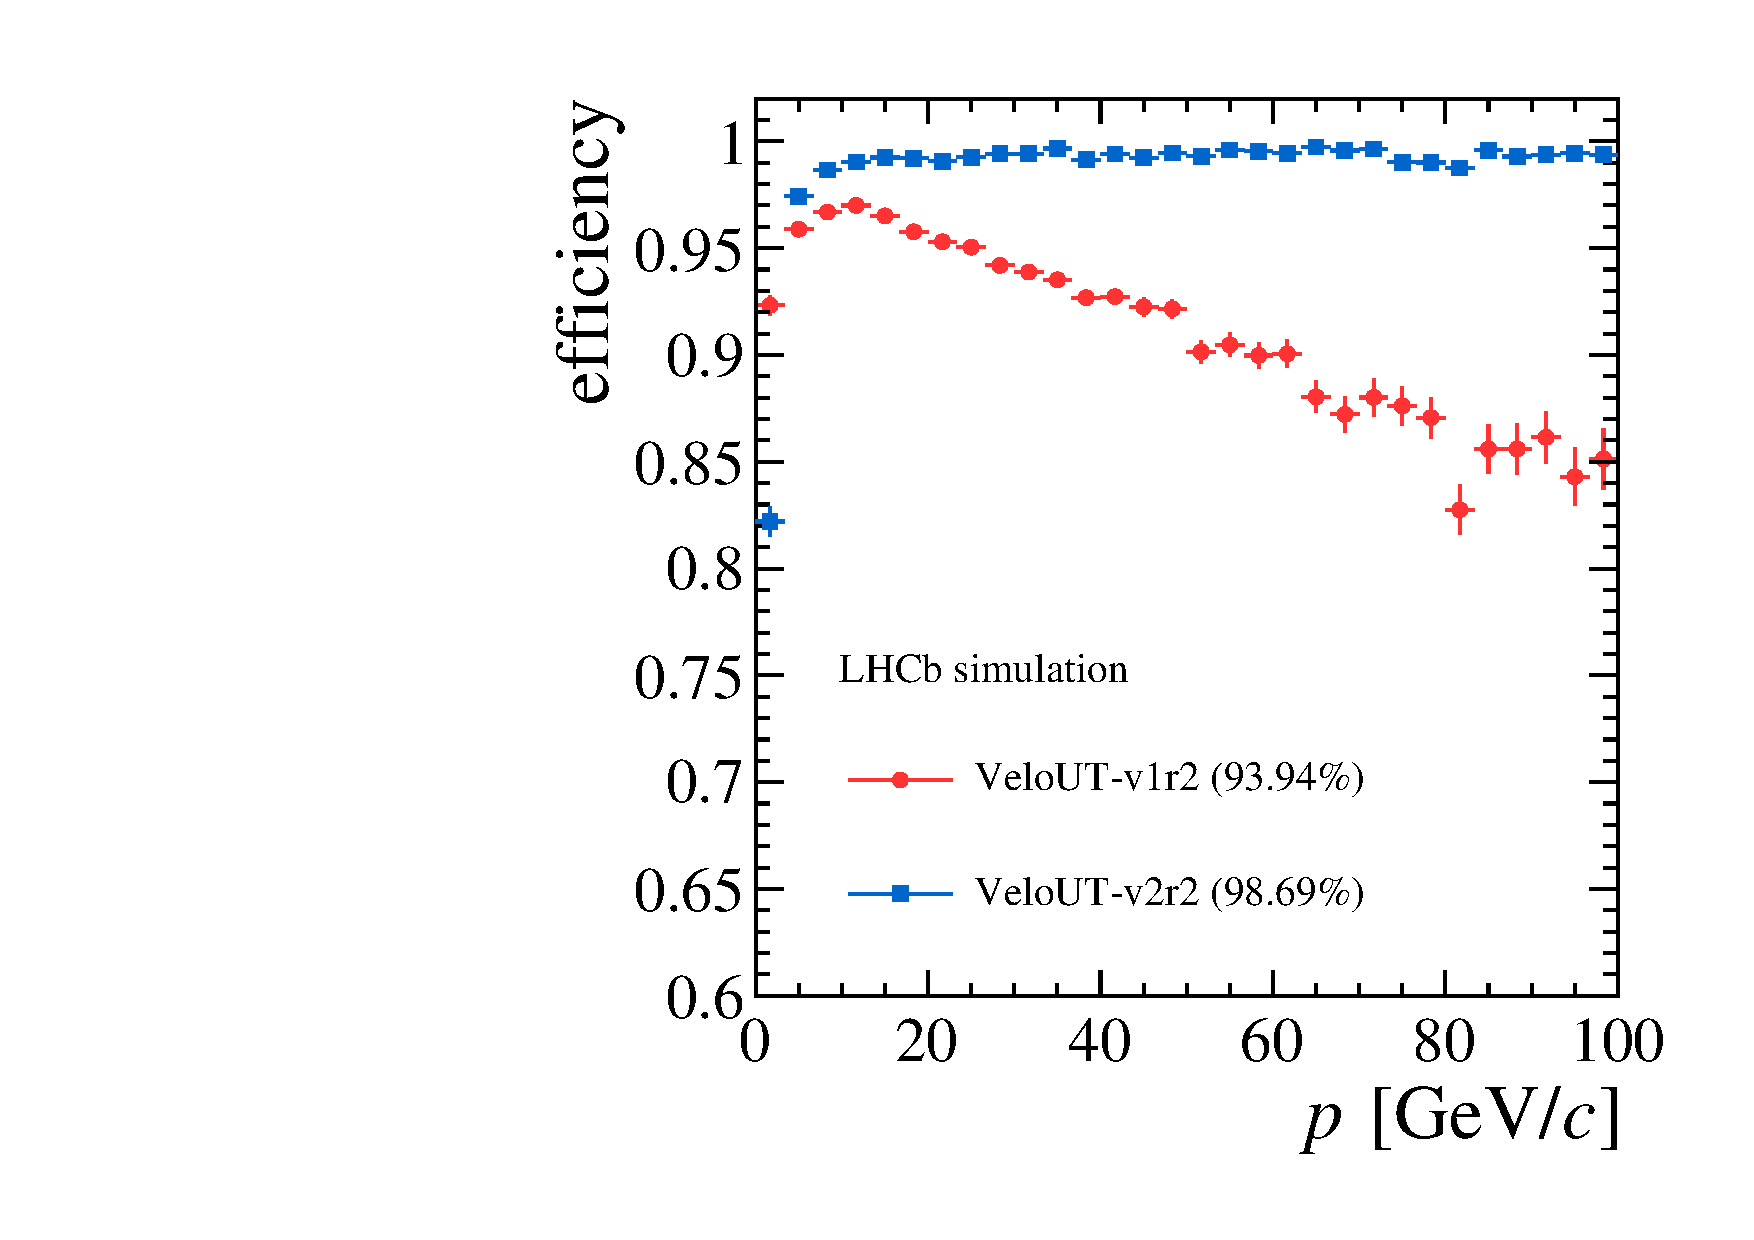
\includegraphics[width=0.45\textwidth]{figs/upstream-tracking-upgrade/eff_p_comp.pdf}
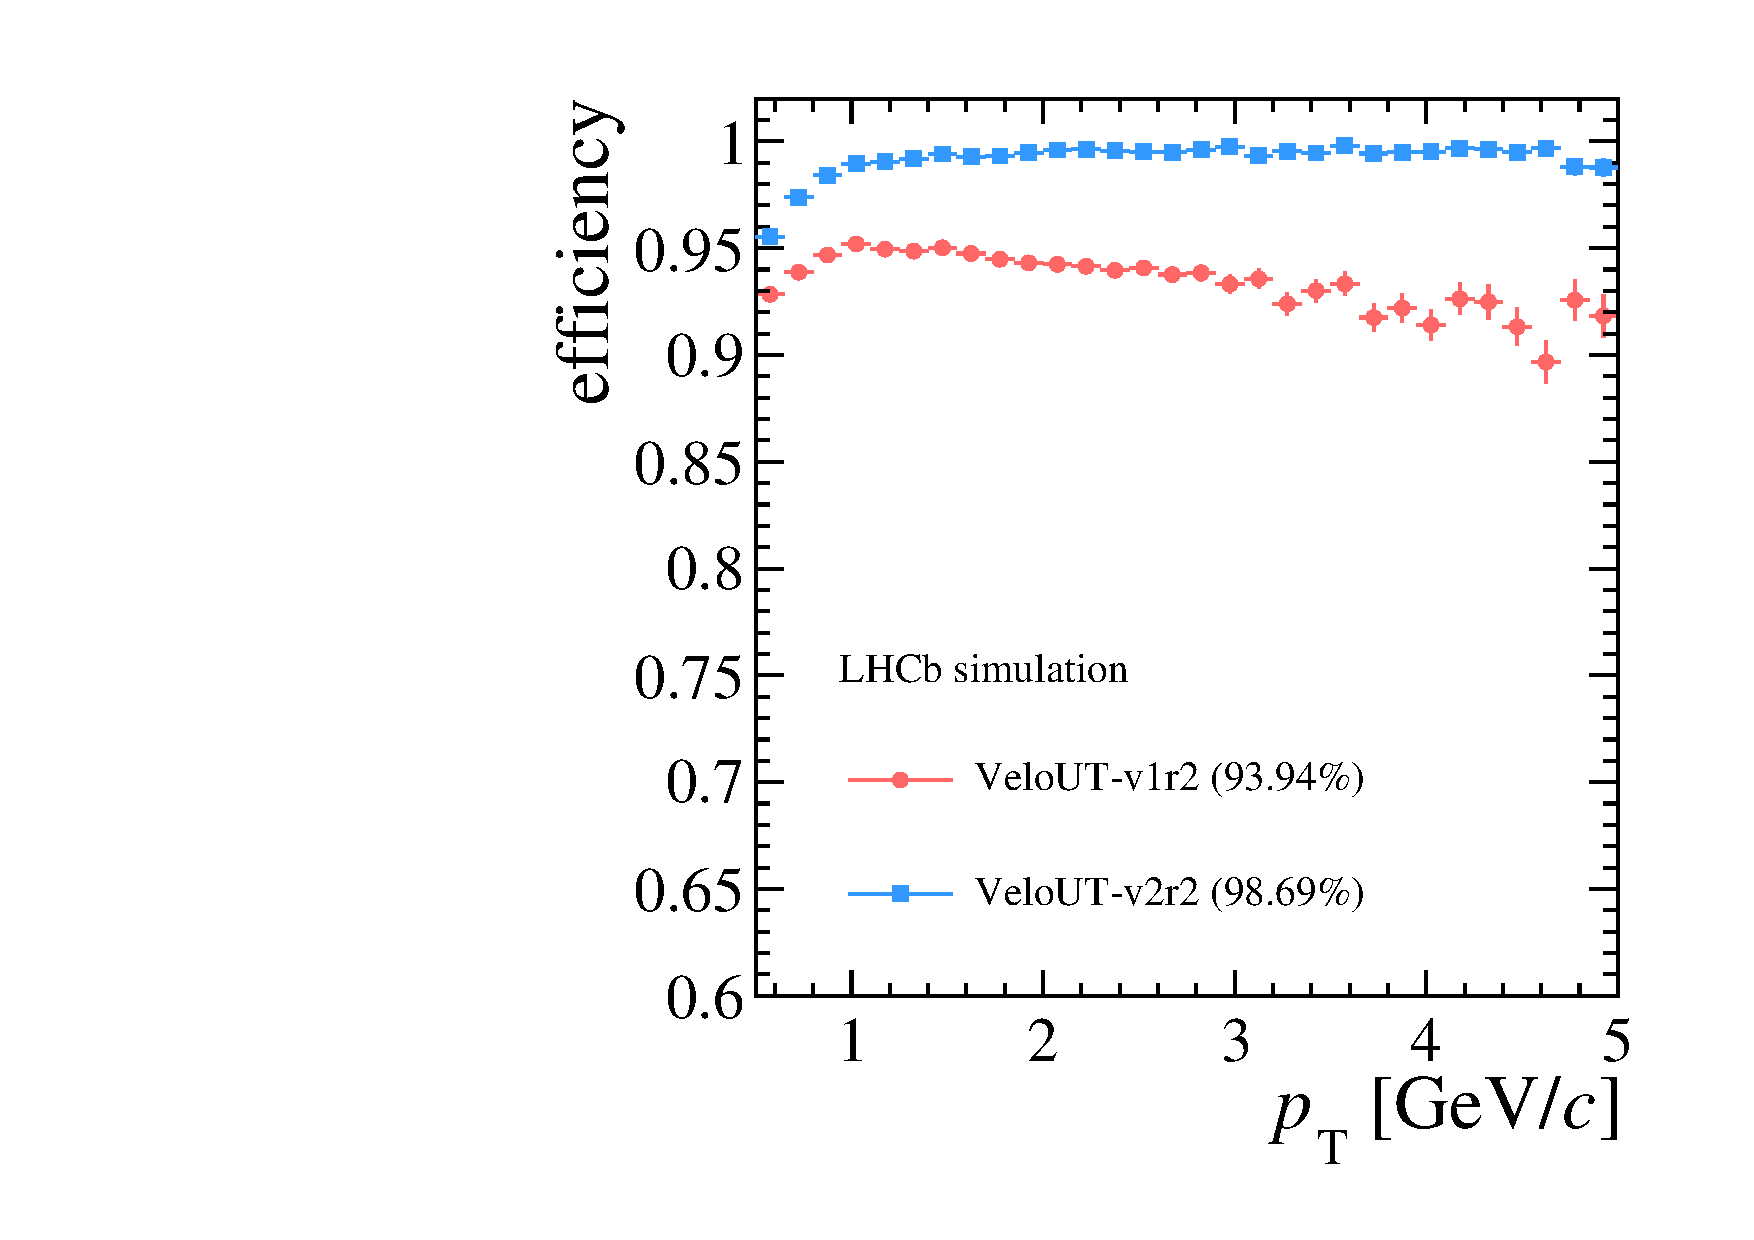
\includegraphics[width=0.45\textwidth]{figs/upstream-tracking-upgrade/eff_pt_comp.pdf}
\caption{The reconstruction efficiency as a function of \ptot and \pt for both the initial version (\texttt{v1r2}) and the optimised version (\texttt{v2r2}) of the \velout algorithm.}
\label{fig:eff_velout_comp}
\end{figure}

\begin{figure}[!tb]
\centering
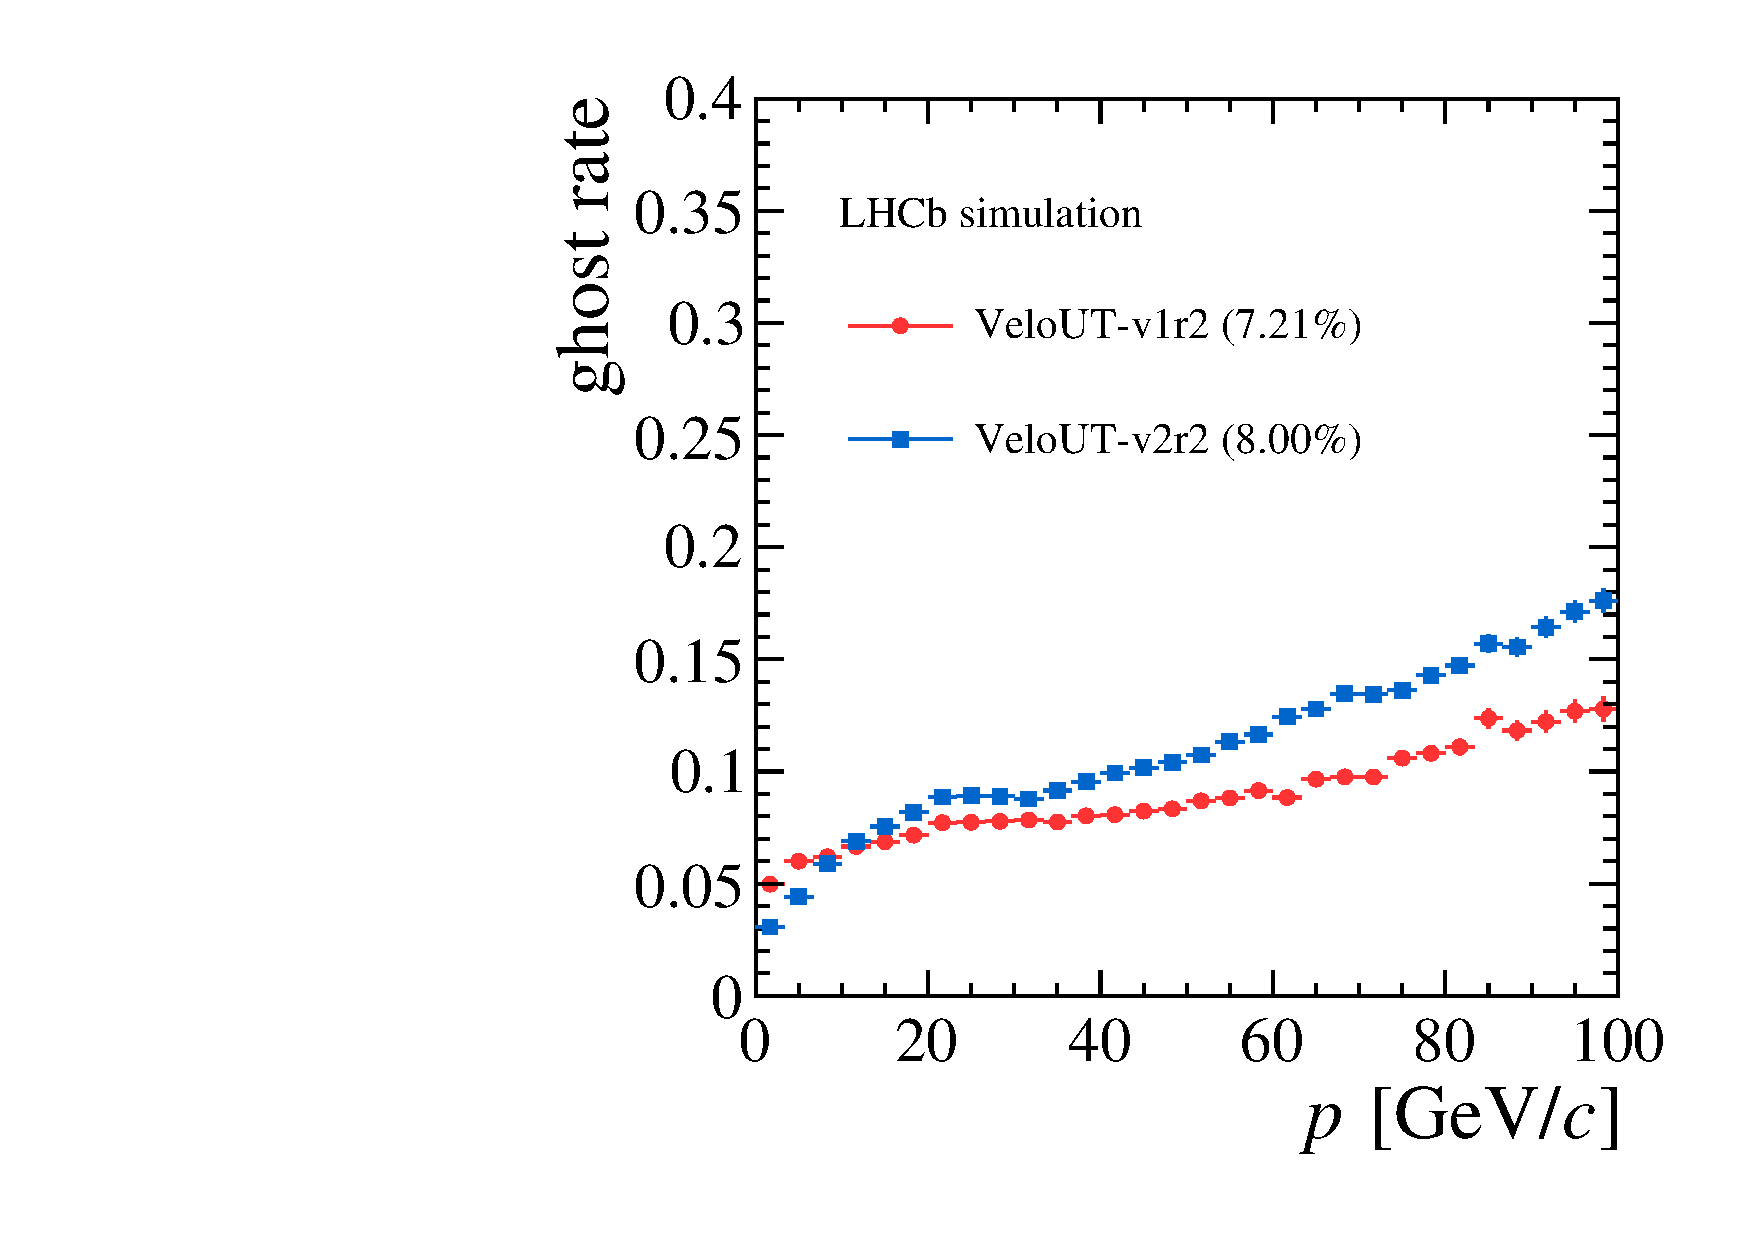
\includegraphics[width=0.45\textwidth]{figs/upstream-tracking-upgrade/gr_p_comp.pdf}
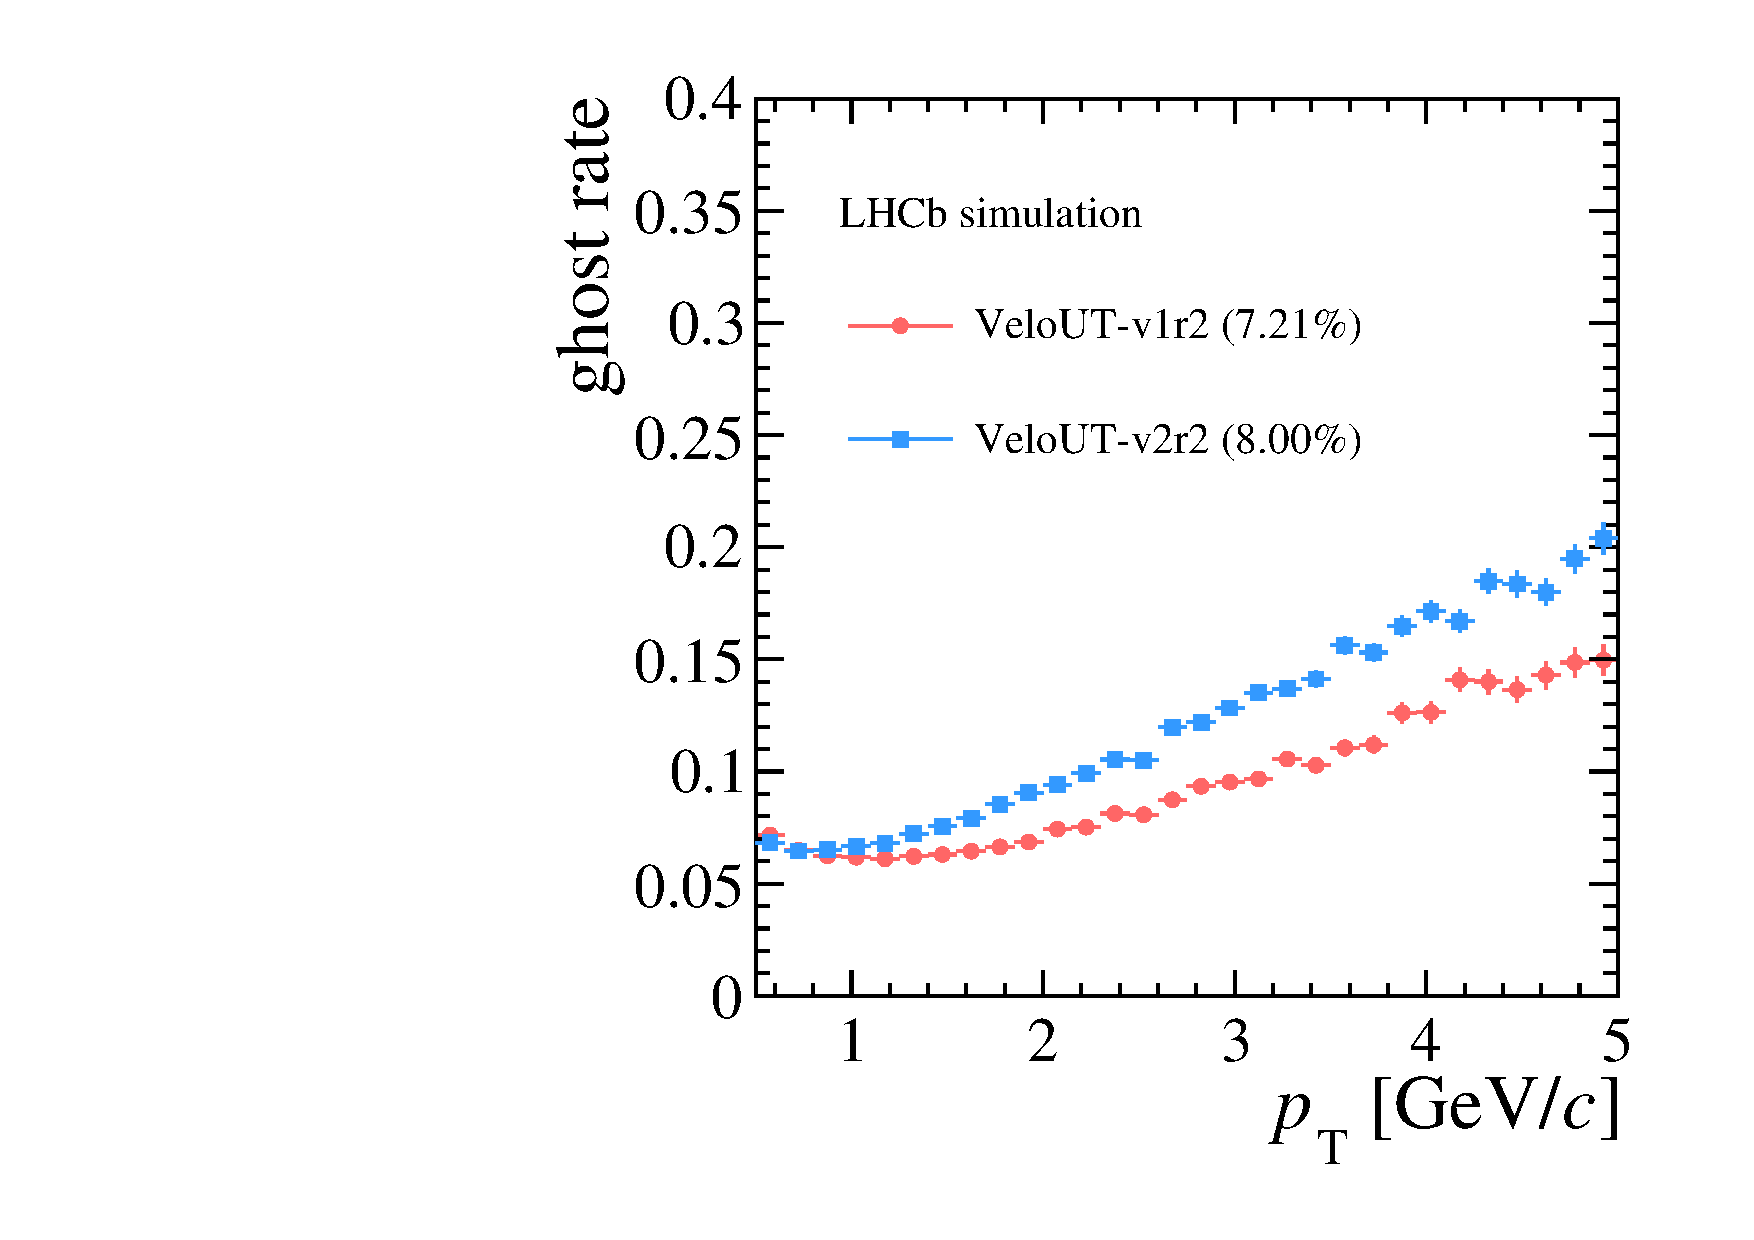
\includegraphics[width=0.45\textwidth]{figs/upstream-tracking-upgrade/gr_pt_comp.pdf}
\caption{The ghost rate as a function of \ptot and \pt for both the initial version (\texttt{v1r2}) and the optimised version (\texttt{v2r2}) of the \velout algorithm.}
\label{fig:gr_velout_comp}
\end{figure}

\subsubsection{Forward}

The track reconstruction efficiency, ghost rate and execution time of the Forward algorithm using \velo or \velout tracks as input are shown in Tab.~\ref{tab:perf_forward_comp}. The track reconstruction efficiency as a function of \ptot and \pt are shown in Fig.~\ref{fig:eff_fwd_comp}. The ghost rate as a function of \ptot and \pt are shown in Fig.~\ref{fig:gr_fwd_comp}. The use of \velout tracks as input to the Forward algorithm drastically reduces the ghost rate and execution time. This comes at a small cost in the track reconstruction efficiency.

\begin{table}[!tb]
\caption{The performances of the Forward algorithm using \velo or \velout tracks as input in terms of track reconstruction efficiency, ghost rate and execution time.}
\resizebox{\columnwidth}{!}{
\begin{tabular}{c|c|c|c|c}
    & Efficiency [\%] & Ghost rate [\%] & VeloUT [ms] & Forward [ms] \\
   \hline
   Velo-Forward  & 94.10  & 41.55  &  -  & 18.28 \\
   VeloUT-Forward  & 93.37  & 14.08  &  0.81 & \hphantom{0}3.45  \\
 \end{tabular}
 }
 \label{tab:perf_forward_comp}
\end{table}

\begin{figure}[!tb]
\centering
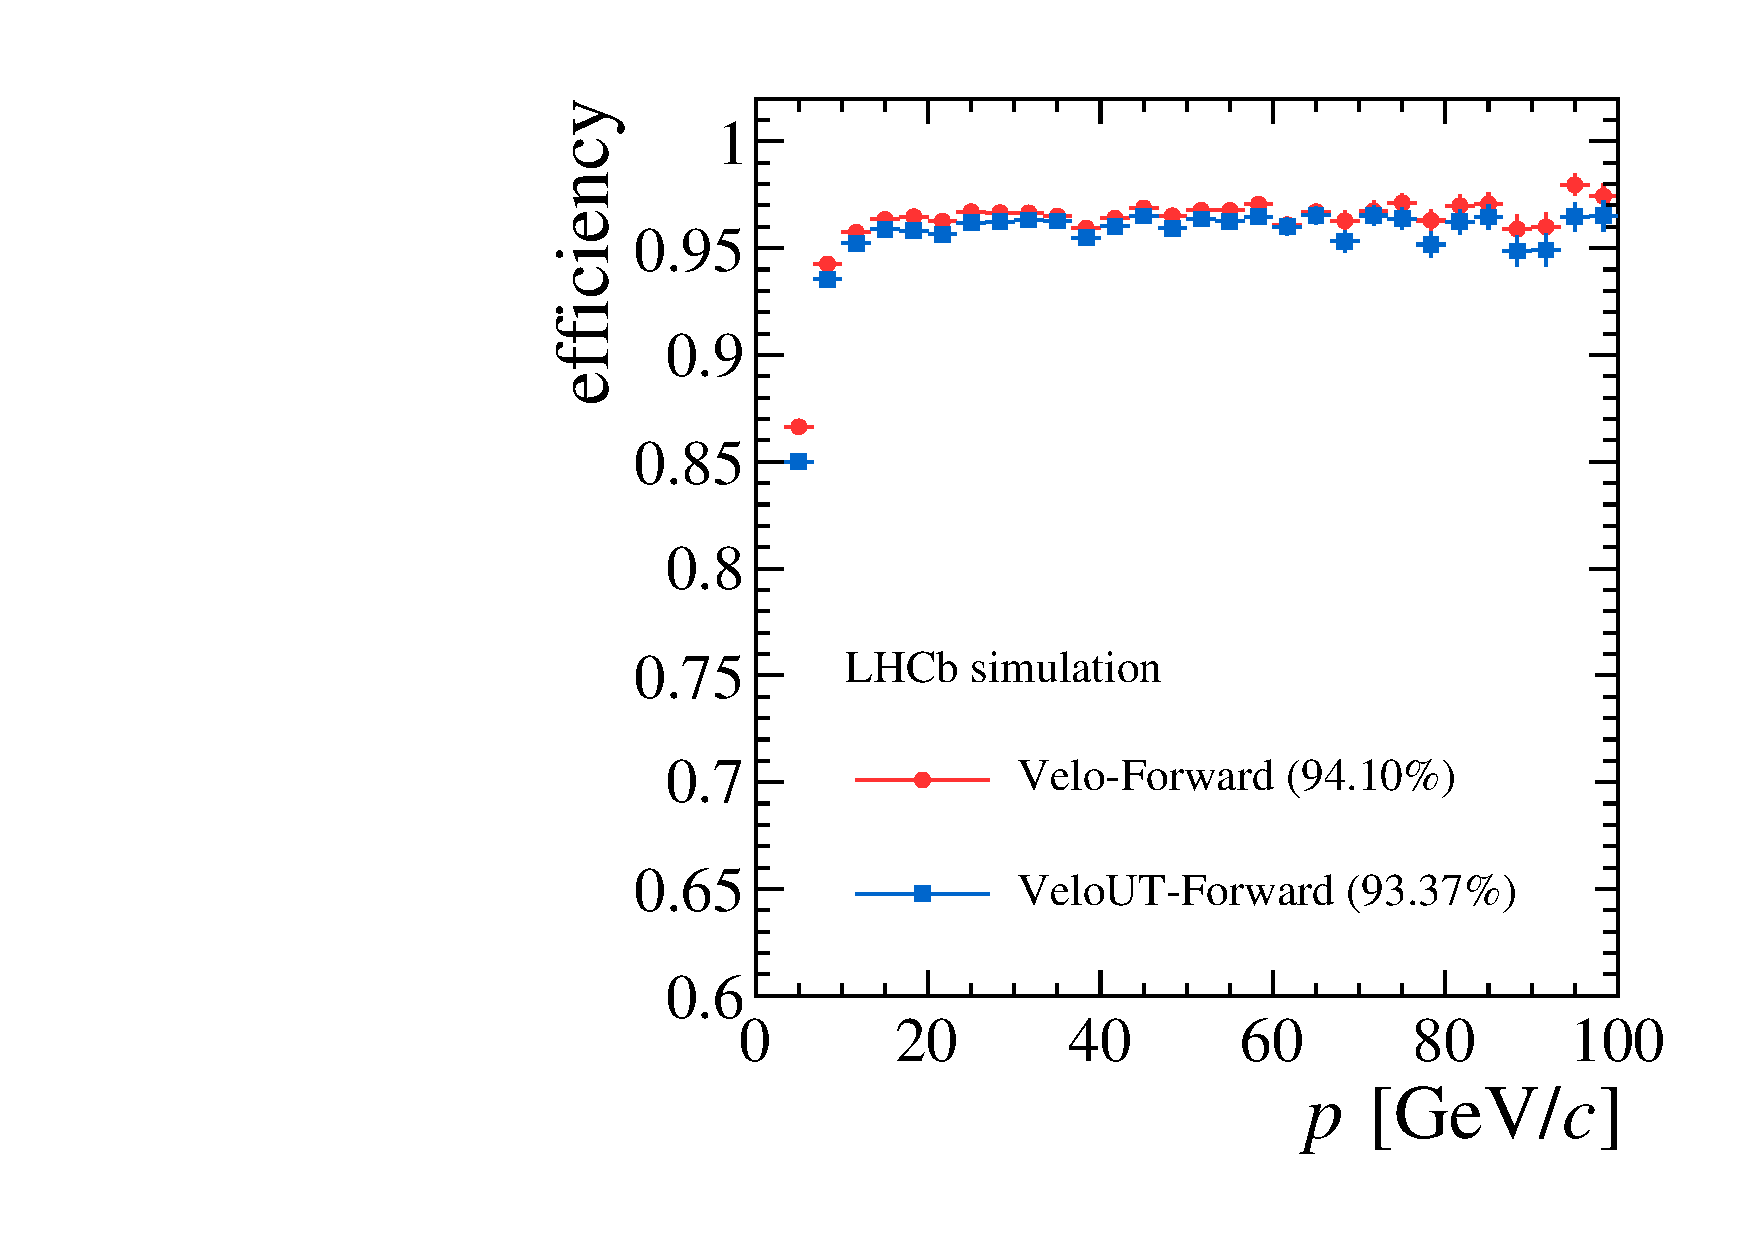
\includegraphics[width=0.45\textwidth]{figs/upstream-tracking-upgrade/fwd_eff_p_comp.pdf}
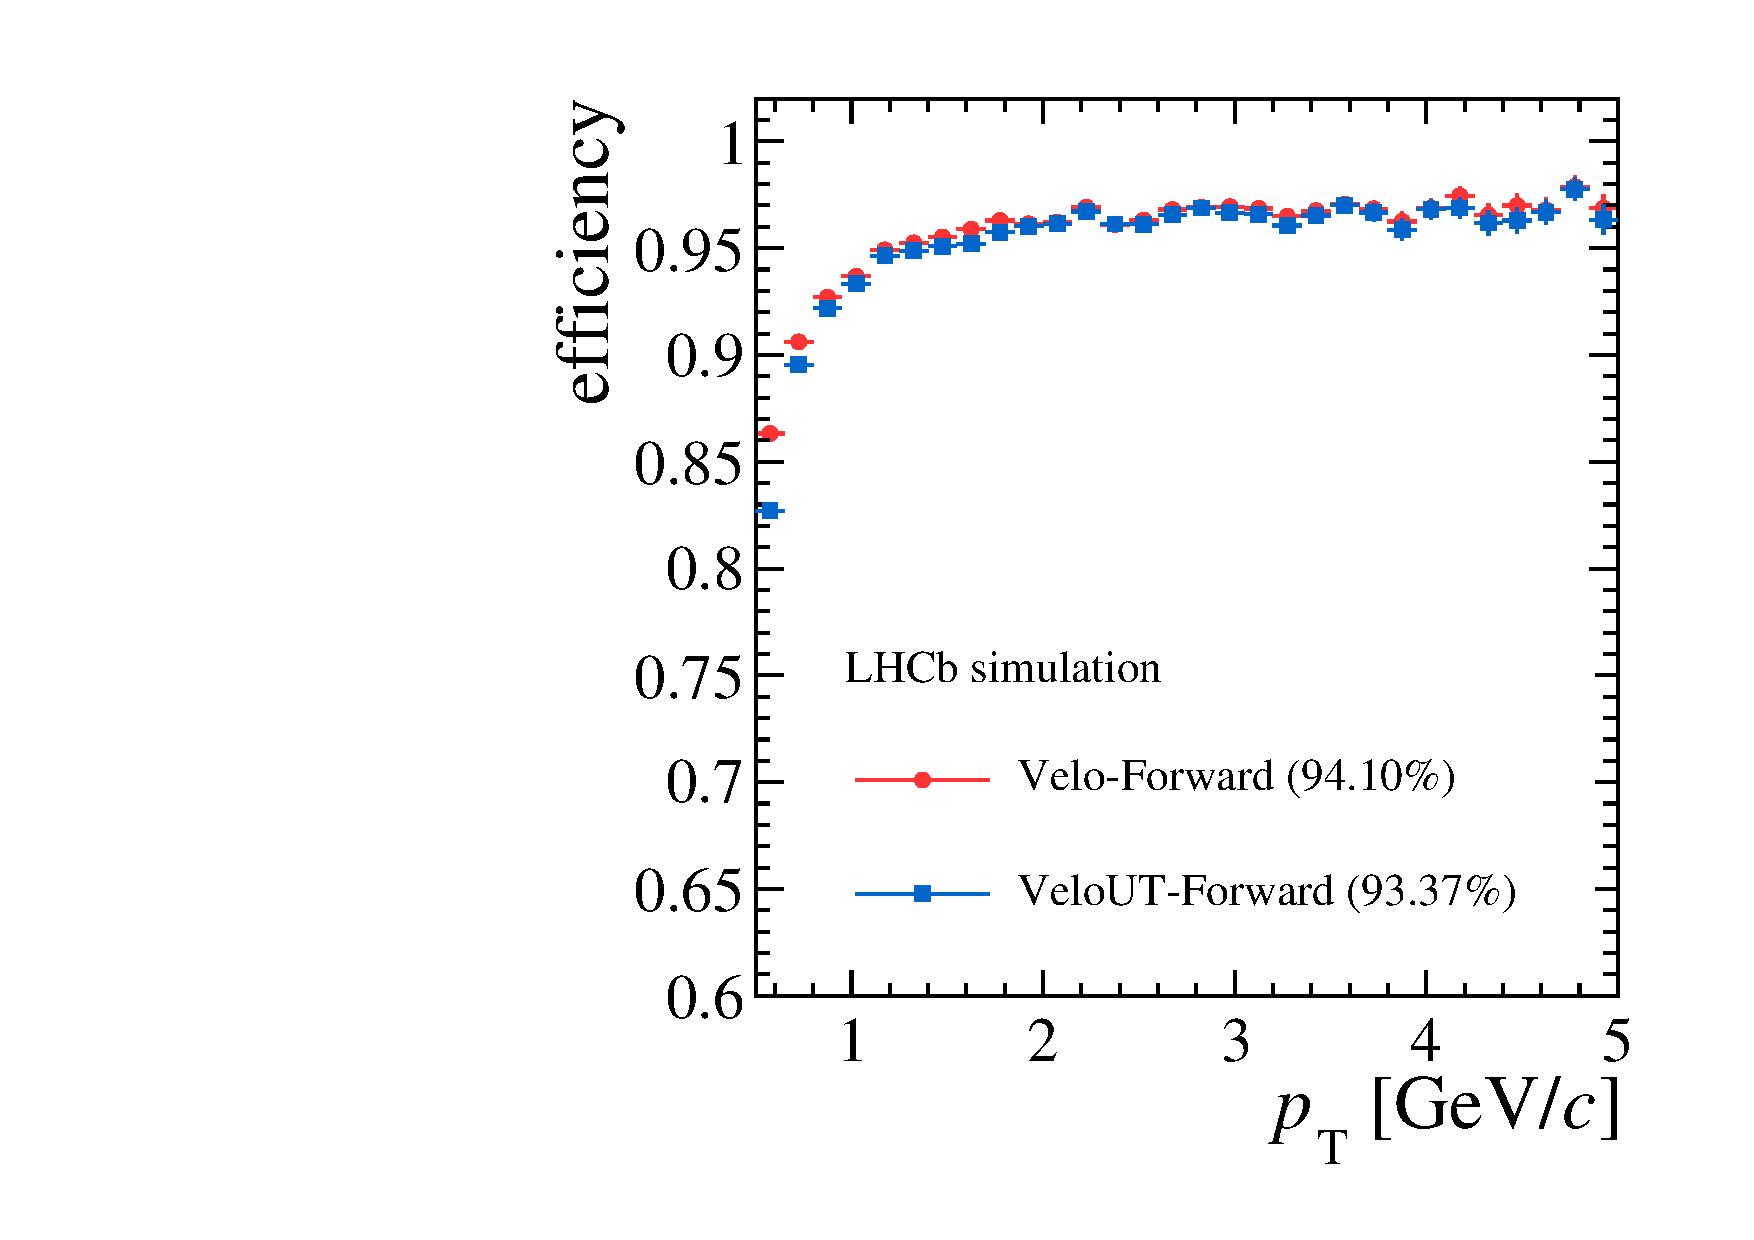
\includegraphics[width=0.45\textwidth]{figs/upstream-tracking-upgrade/fwd_eff_pt_comp.pdf}
\caption{The track reconstruction efficiency of the Forward algorithm using \velo or \velout tracks as a function of \ptot and \pt.}
\label{fig:eff_fwd_comp}
\end{figure}

\begin{figure}[!tb]
\centering
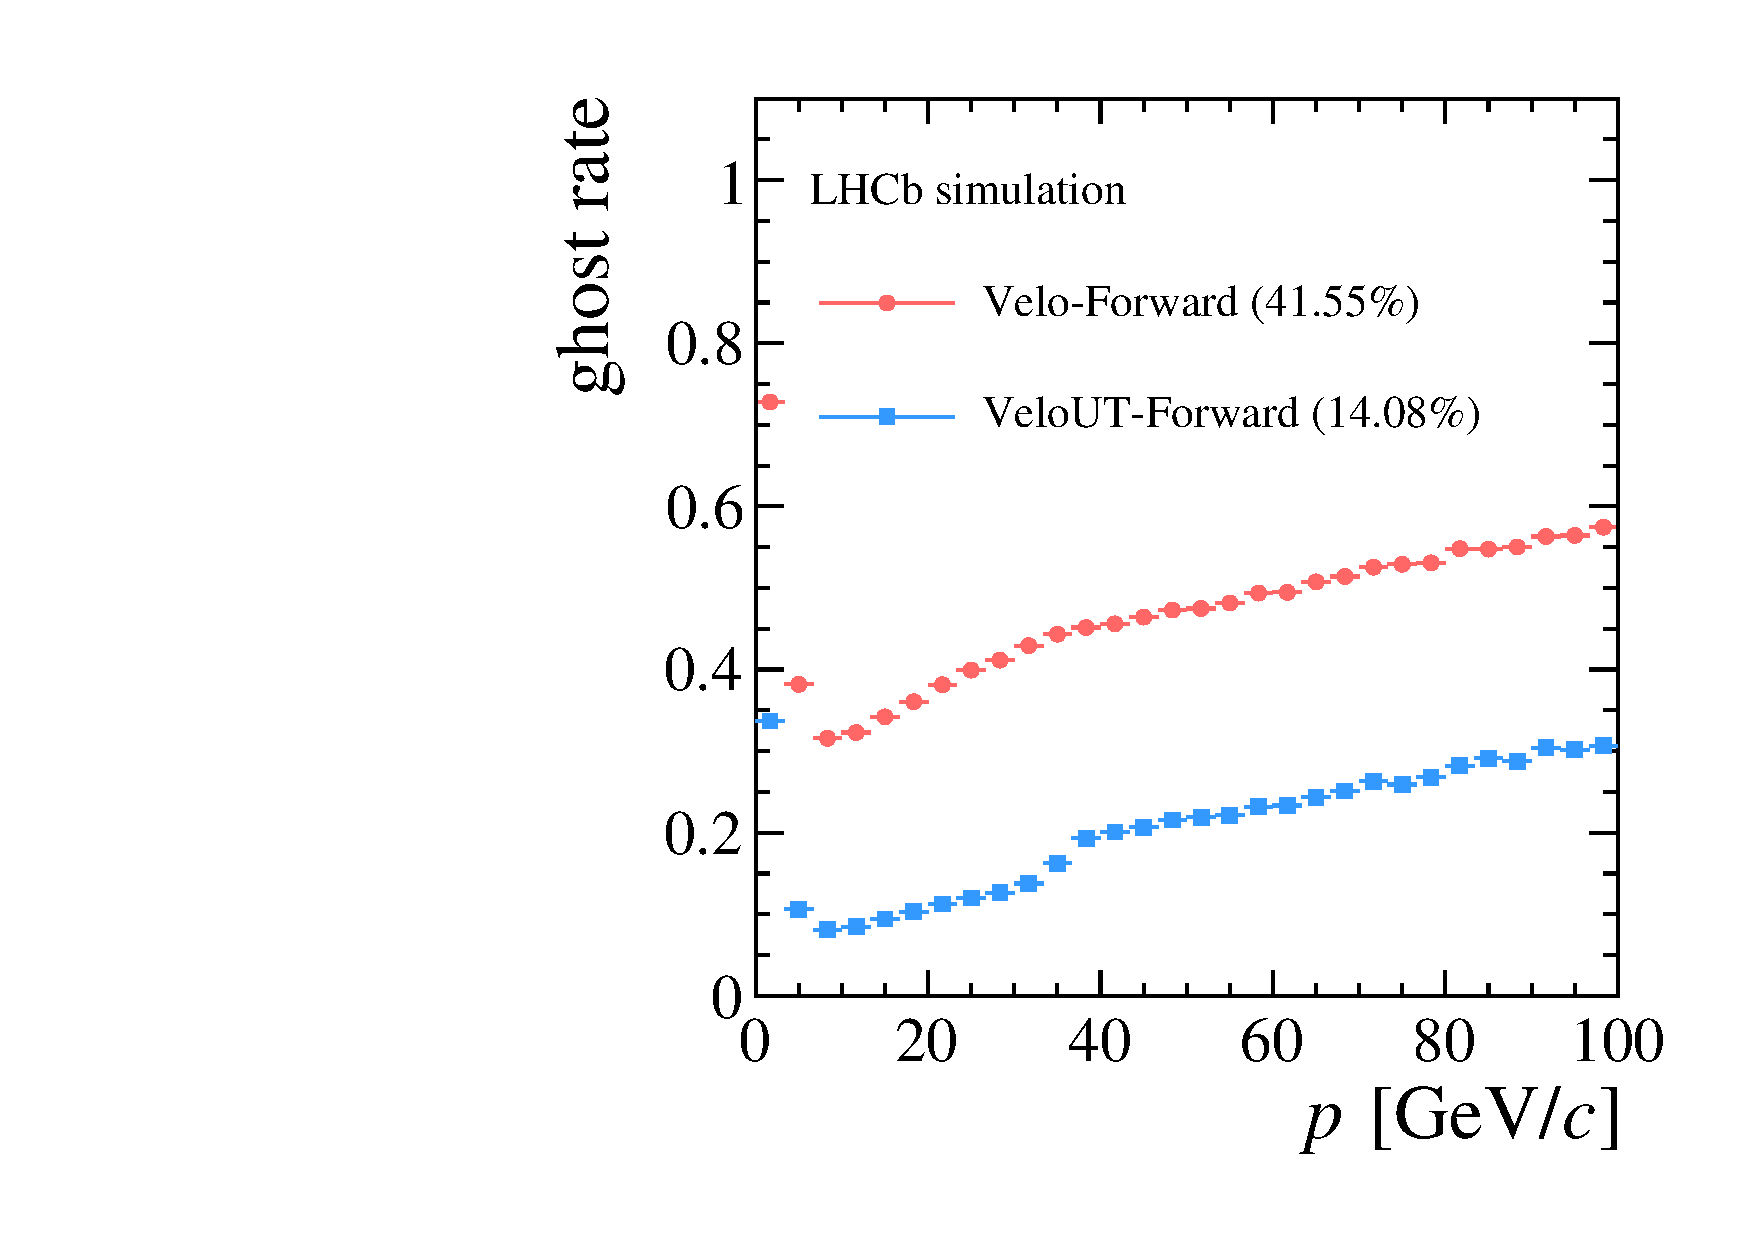
\includegraphics[width=0.45\textwidth]{figs/upstream-tracking-upgrade/fwd_gr_p_comp.pdf}
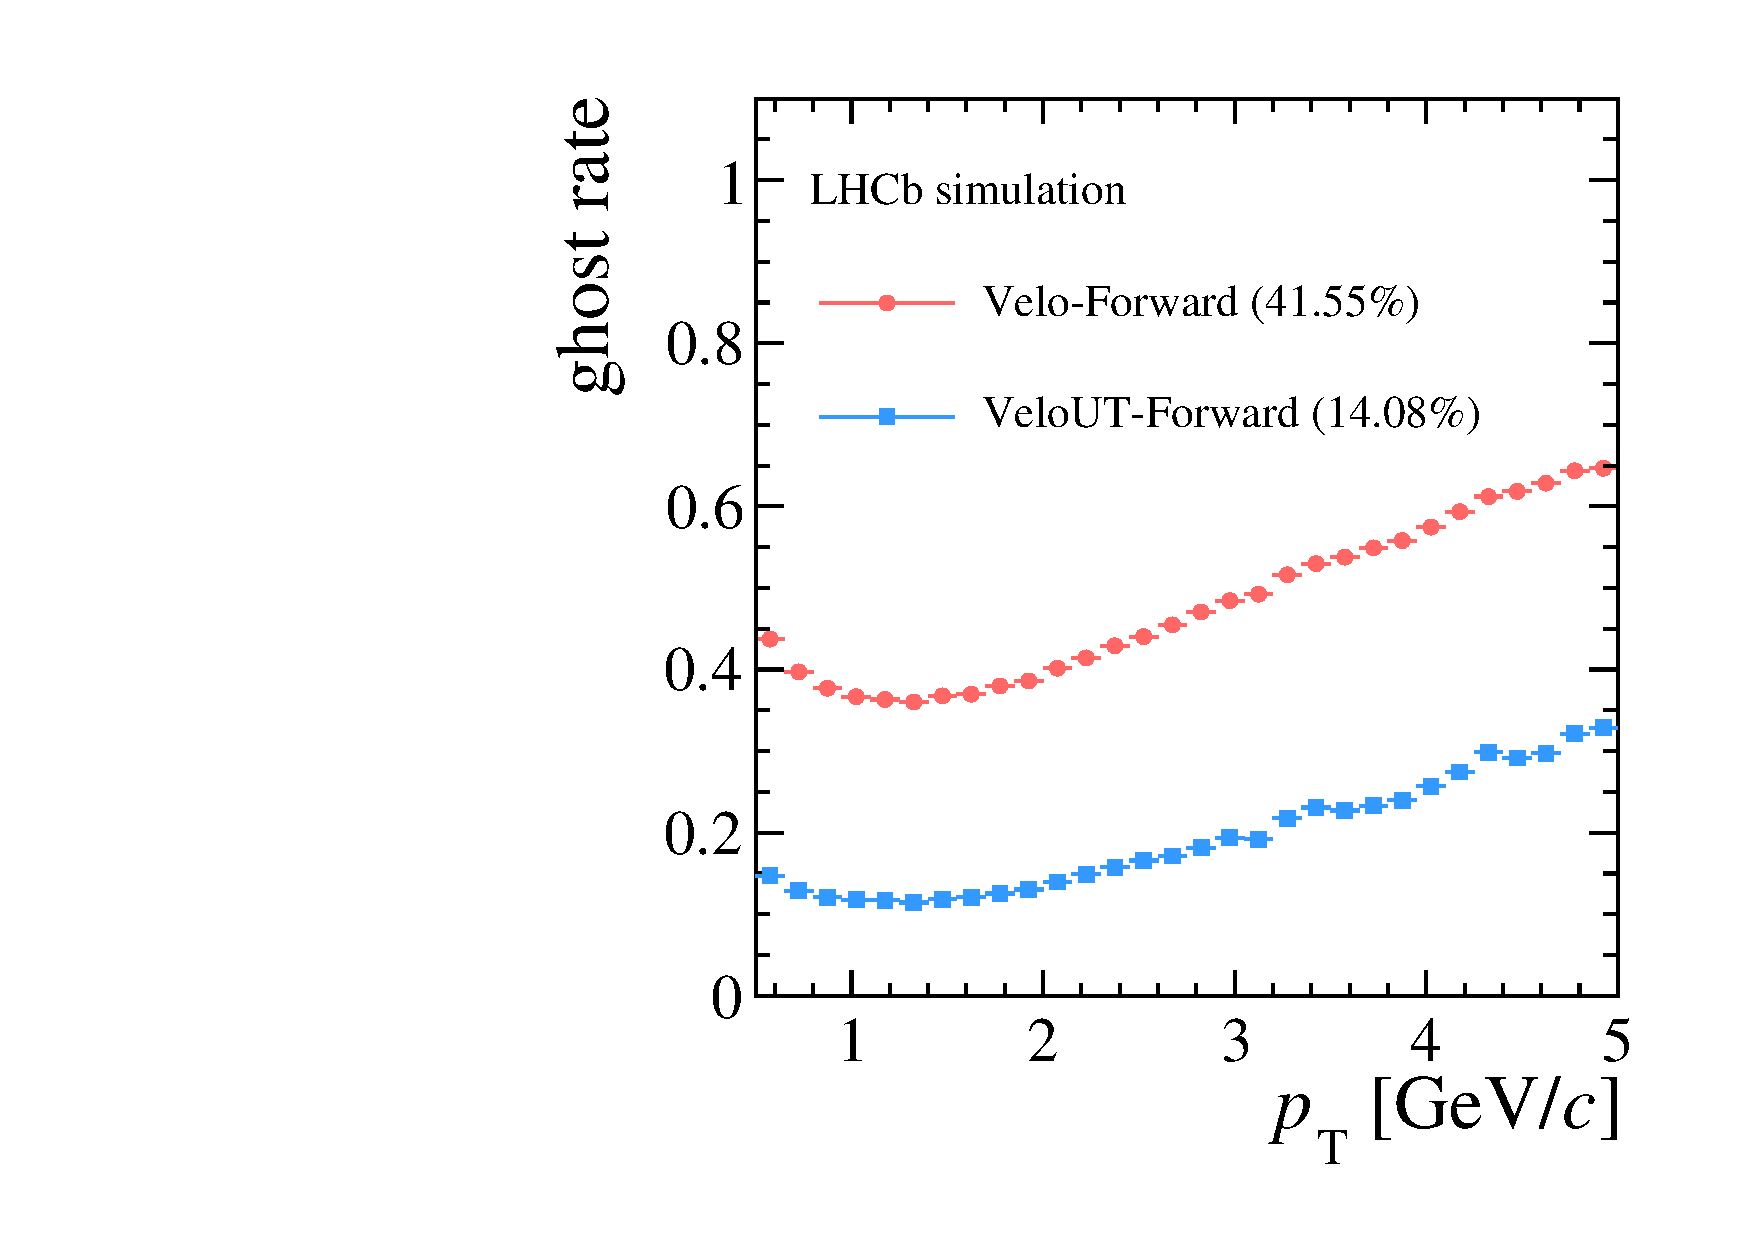
\includegraphics[width=0.45\textwidth]{figs/upstream-tracking-upgrade/fwd_gr_pt_comp.pdf}
\caption{The ghost rate of the Forward algorithm using \velo or \velout tracks as a function of \ptot and \pt.}
\label{fig:gr_fwd_comp}
\end{figure}

\subsection{Summary}

The vast improvements in the performance of the \velout and the subsequent improvement to the overall tracking sequence led to the algorithm being adopted into the default tracking sequence for the \lhcb Upgrade~\cite{upgrade-tracker-tdr,upgrade-trigger-tdr}. It will play a large role in allowing \lhcb to become the first hadron collider experiment to operate a software-only trigger at the full event rate.


\clearpage
\section{Upstream tracking for the \lhcb Run II}
\label{sec:up-track-run2}

\subsection{Motivation}

Following the improved performance achieved using \velout tracks within the tracking sequence of the \lhcb Upgrade, outlined in Sec.~\ref{sec:up-track-upgrade}, a similar strategy was developed for Run II. This strategy involved using \velott tracks as input for the Forward tracking at the first stage of the software trigger. A new \velott algorithm for Run II~\cite{velott} was created based on the \velout algorithm, taking into account the slight differences in geometry between the two detectors. In the following, the improved performance for the \velott algorithm for Run II compared to Run I will be shown along with the improved performance achieved when using \velott tracks rather than \velo tracks as input to the Forward tracking algorithm.

\subsection{Performance}

\subsubsection{VeloTT}

The track reconstruction efficiency, ghost rate and execution time of the VeloTT algorithm for Run I and Run II are shown in Table~\ref{tab:perf_velott_comp}. The track reconstruction efficiency as a function of \ptot and \pt are shown in Fig.~\ref{fig:eff_velott_comp}. The ghost rate as a function of \ptot and \pt are shown in Fig.~\ref{fig:gr_velott_comp}. The Run II implementation shows large improvements in terms of track reconstruction efficiency and execution time. The increased track reconstruction efficiency is most evident at high \ptot as the Run I implementation shows a negative trend for increasing \ptot. There is also a slight increase in the ghost rate. However, this is of lesser importance as the ghost rate can be further reduced during offline analysis. 

\begin{table}[!b]
\caption{The performances of the VeloTT algorithms for Run I and Run II in terms of track reconstruction efficiency, ghost rate and execution time.}
\label{tab:perf_velott_comp}
\begin{center}
  \begin{tabular}{c|c|c|c}
    VeloTT & Efficiency [\%] & Ghost rate [\%] & Timing [ms] \\ 
    \hline
    Run I  &  92.74  &  \hphantom{0}7.21  &  32.50  \\ 
    Run II  &  97.77  &  11.60  &  \hphantom{0}0.50   \\ 
  \end{tabular}
\end{center}
\end{table}

\begin{figure}[!tb]
\begin{center}
  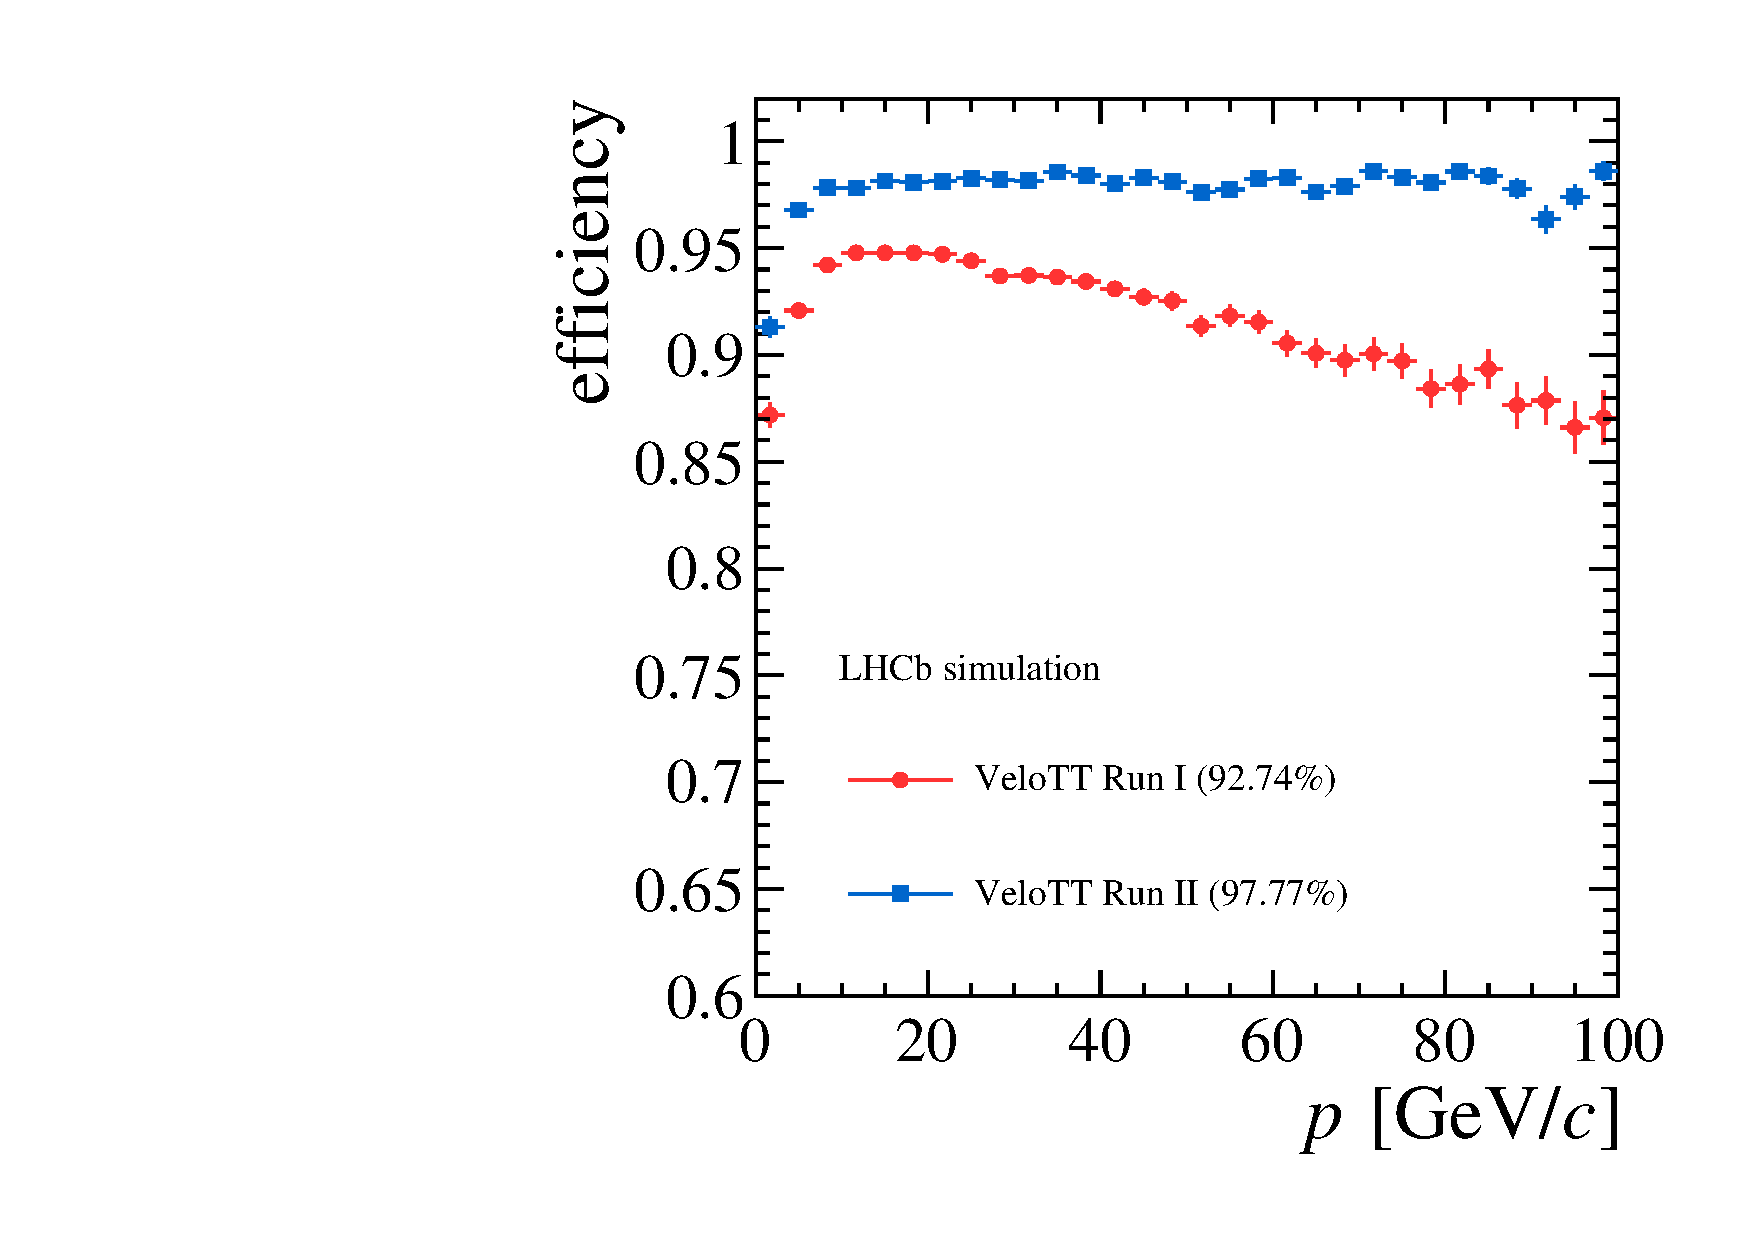
\includegraphics[width=0.45\linewidth]{figs/upstream-tracking-run2/VeloTT-eff-p.pdf}
  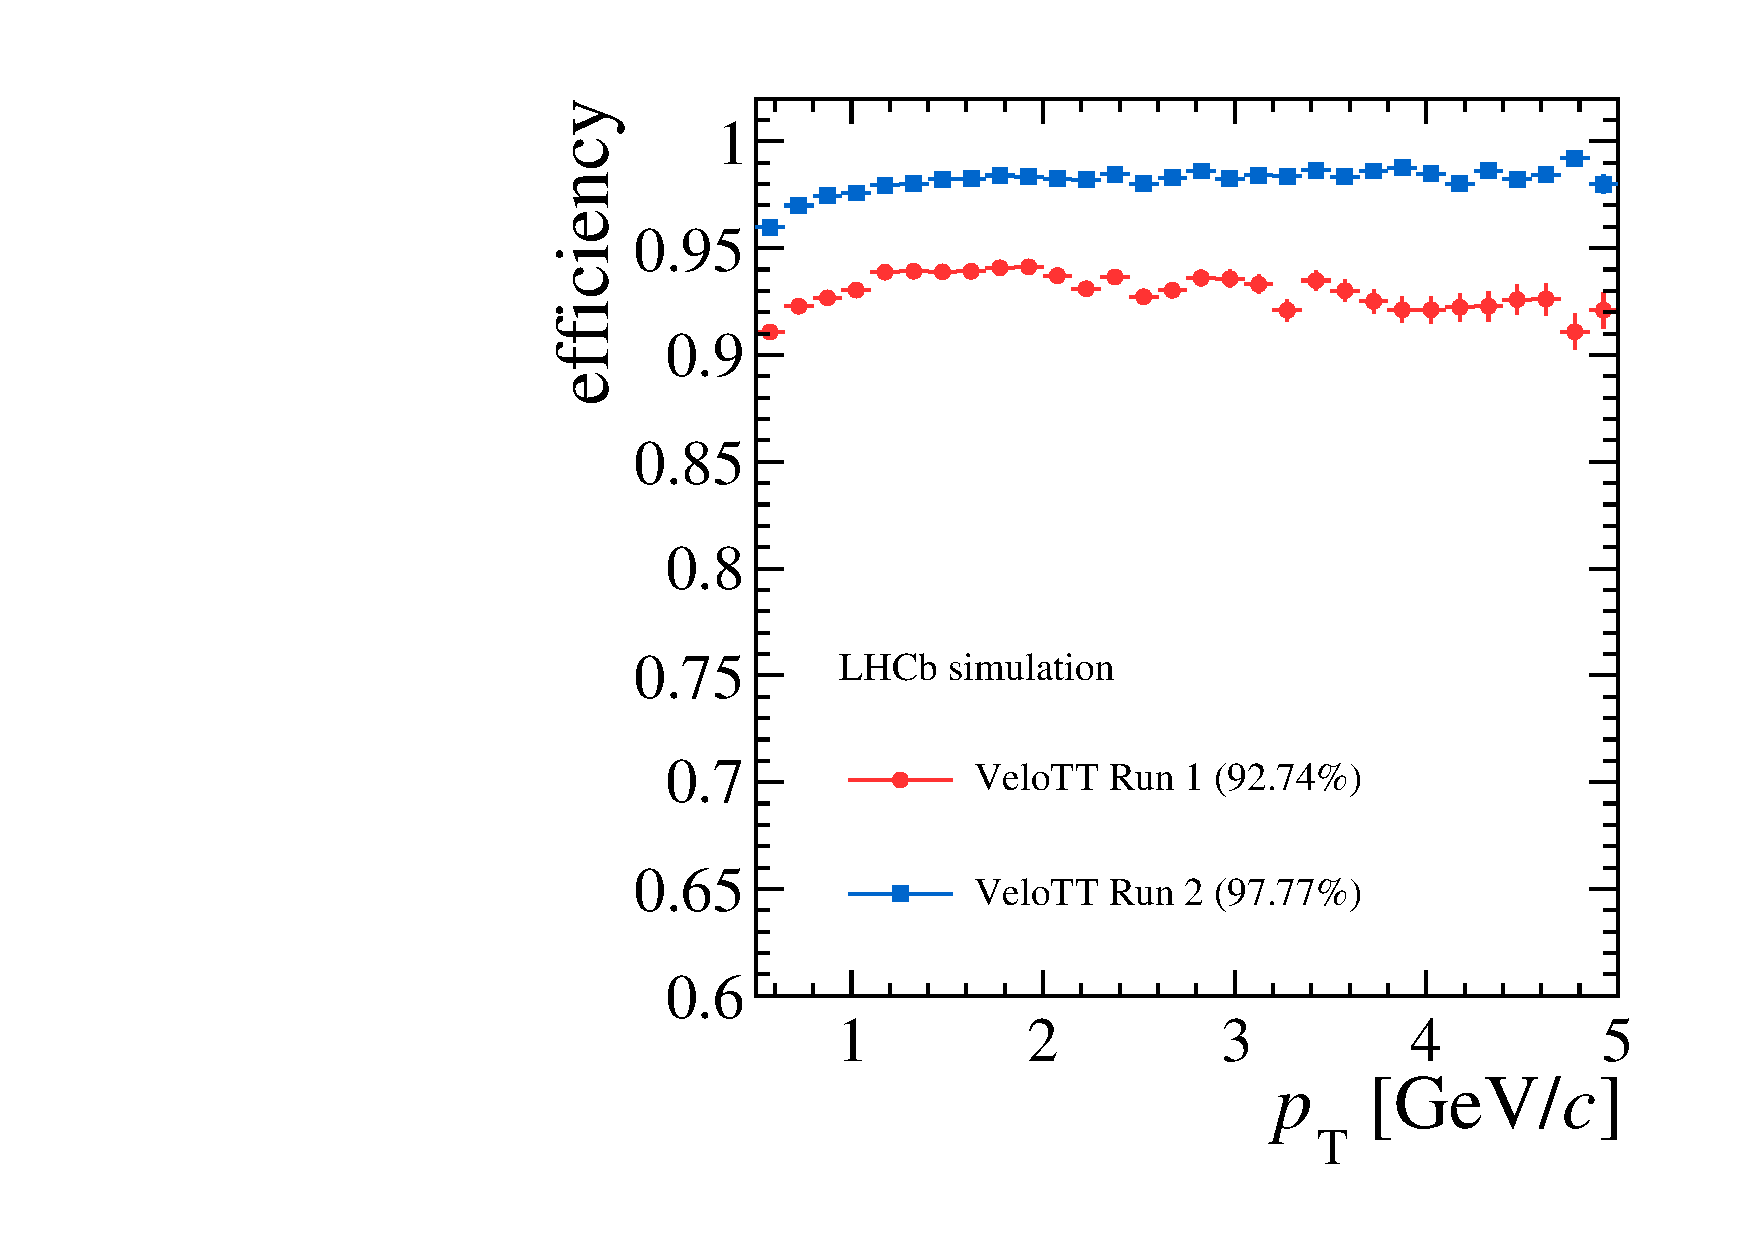
\includegraphics[width=0.45\linewidth]{figs/upstream-tracking-run2/VeloTT-eff-pt.pdf}
  \caption{The track reconstruction efficiency of the VeloTT algorithms for Run I and Run II as a function of \ptot and \pt.}
  \label{fig:eff_velott_comp}
  \end{center}
\end{figure}

\begin{figure}[!tb]
  \begin{center}
    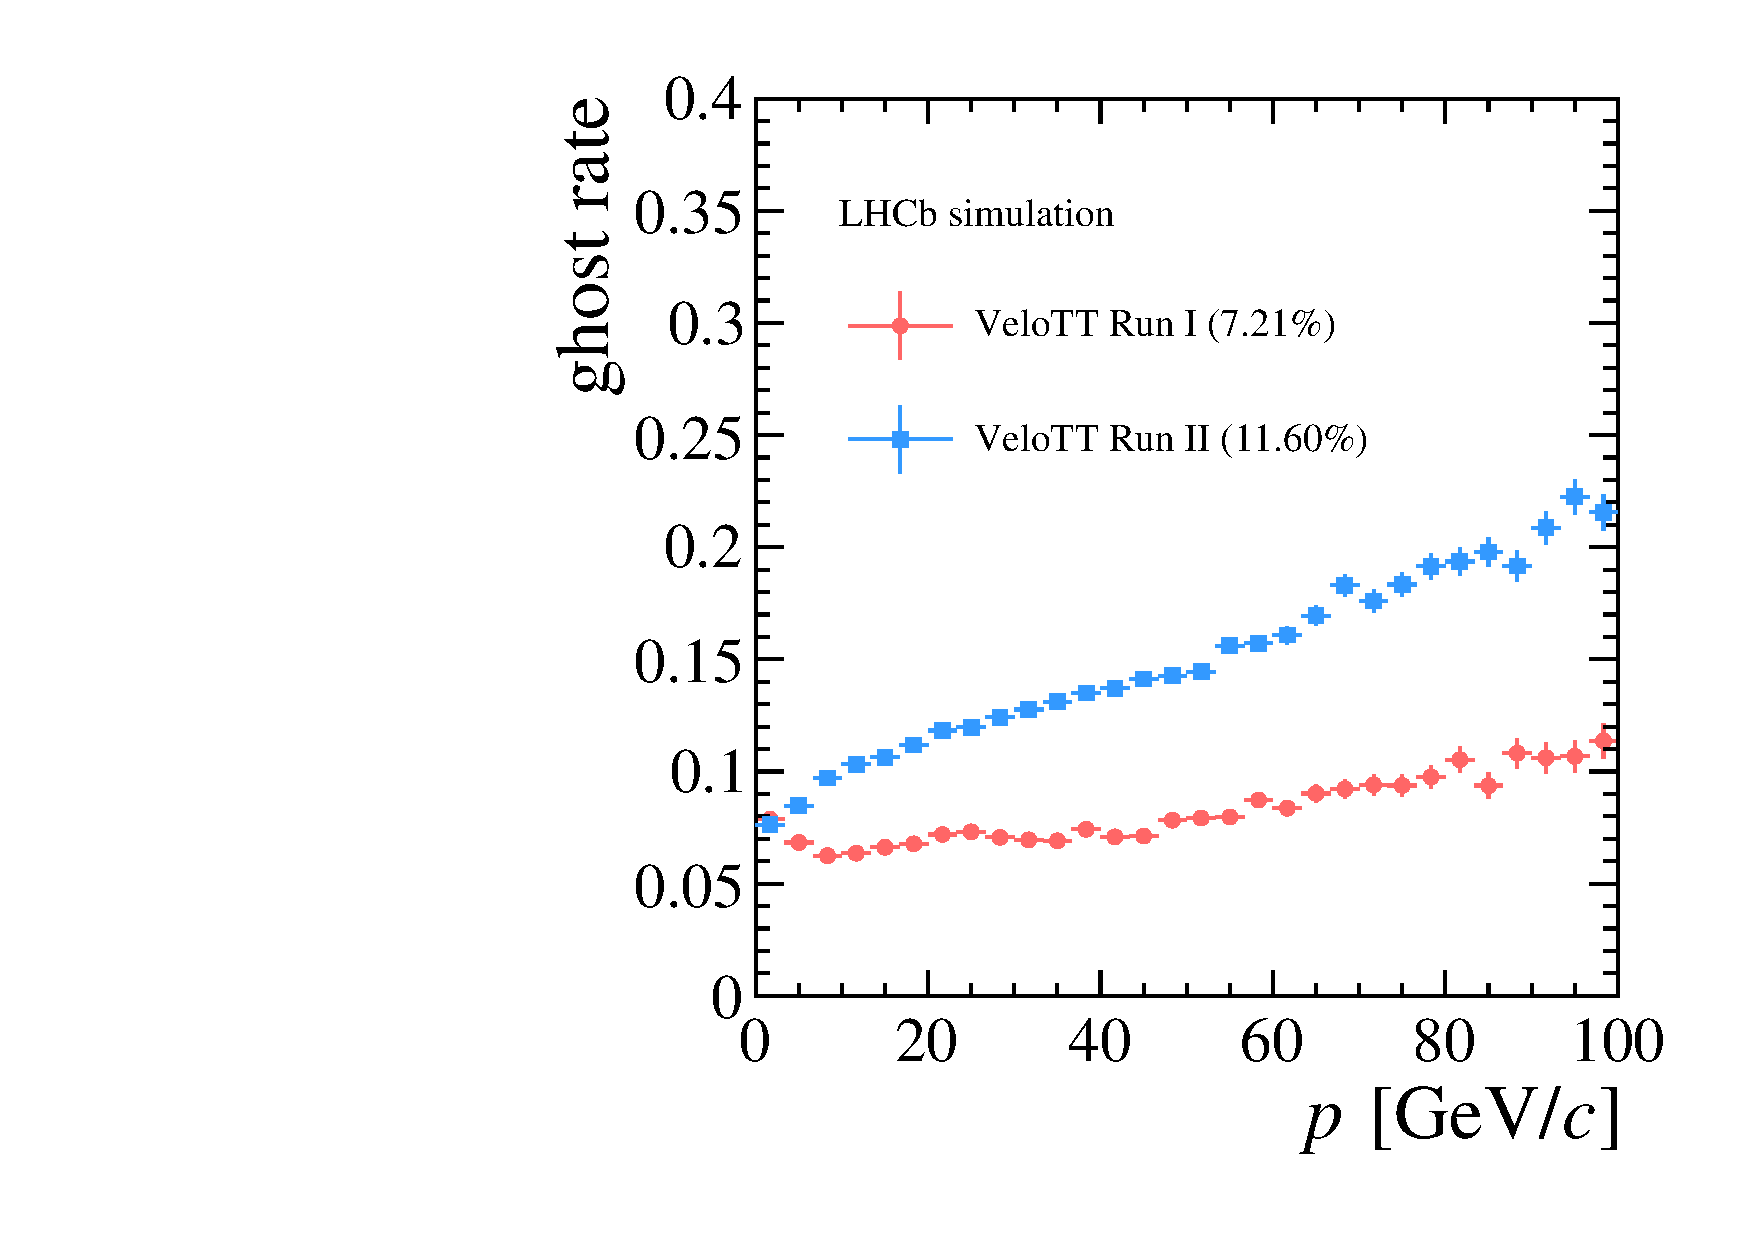
\includegraphics[width=0.45\linewidth]{figs/upstream-tracking-run2/VeloTT-gr-p.pdf}
    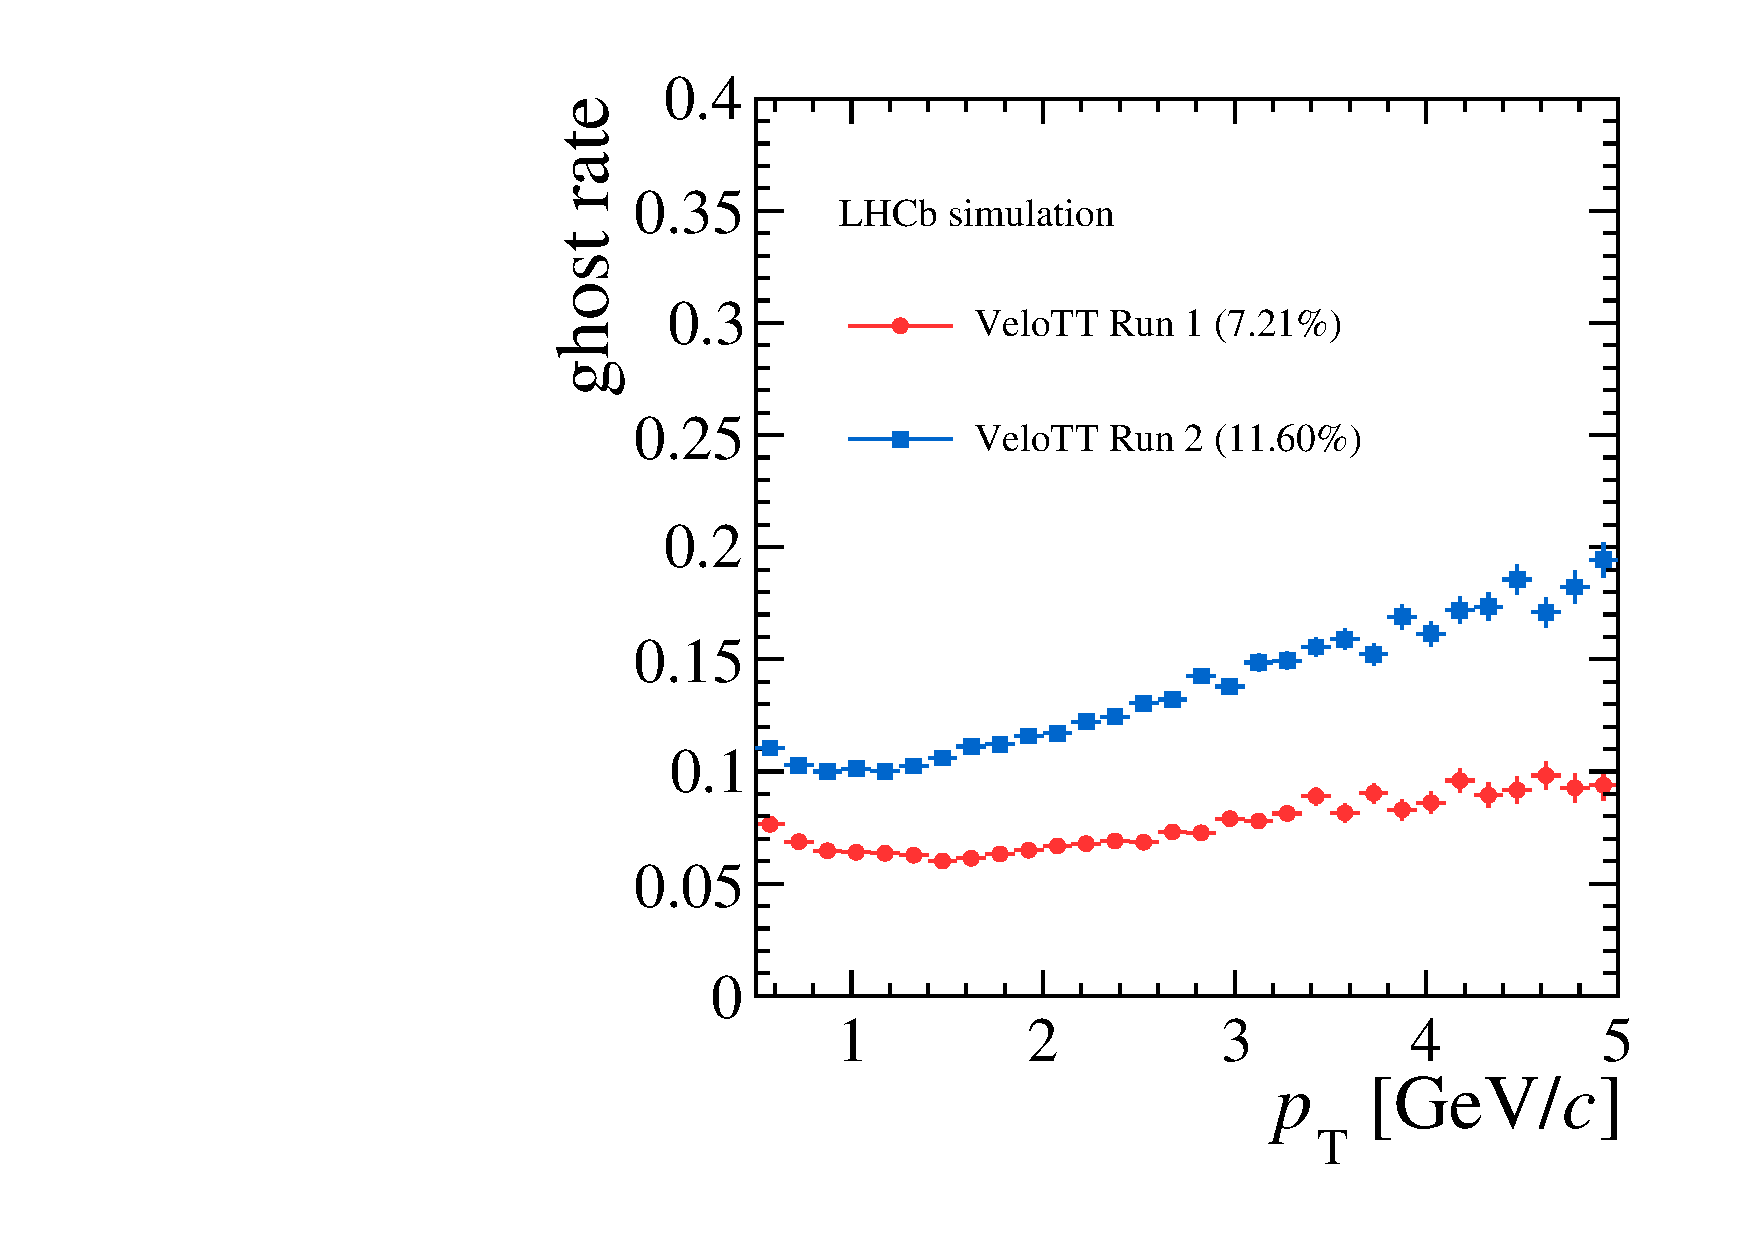
\includegraphics[width=0.45\linewidth]{figs/upstream-tracking-run2/VeloTT-gr-pt.pdf}
    \caption{The ghost rate of the VeloTT algorithms for Run I and Run II as a function of \ptot and \pt.}
    \label{fig:gr_velott_comp}
  \end{center}
\end{figure}

\subsubsection{Forward}

The track reconstruction efficiency, ghost rate and execution time of the Forward algorithm taking \velo or VeloTT tracks as input are shown in Table~\ref{tab:perf_forward_run2_comp}. The track reconstruction efficiency as a function of \ptot and \pt are shown in Fig.~\ref{fig:eff_forward_run2_comp}. The ghost rate as a function of \ptot and \pt are shown in Fig.~\ref{fig:gr_forward_run2_comp}. The use of VeloTT tracks as input drastically reduces the ghost rate and execution time of the Forward algorithm. This comes at a small cost the in track reconstruction efficiency. This efficiency is retrieved in the second stage of the software trigger~\cite{hlt-runII}.

\begin{table}[!tb]
  \caption{The performances of the Forward algorithm using \velo or VeloTT tracks as input in terms of track reconstruction efficiency, ghost rate and execution time.}
  \label{tab:perf_forward_run2_comp}
  \begin{center}
    \begin{tabular}{c|c|c|c|c}
      & Efficiency [\%] & Ghost rate [\%] & VeloTT [ms] & Forward [ms] \\ 
      \hline
      Velo-Forward  & 93.15  & 46.86  &  -  & 13.71 \\ 
      VeloTT-Forward  & 89.23  & 17.13  &  0.50 & \hphantom{0}4.08 \\
    \end{tabular}
  \end{center}
\end{table}

\begin{figure}[!tb]
  \begin{center}
    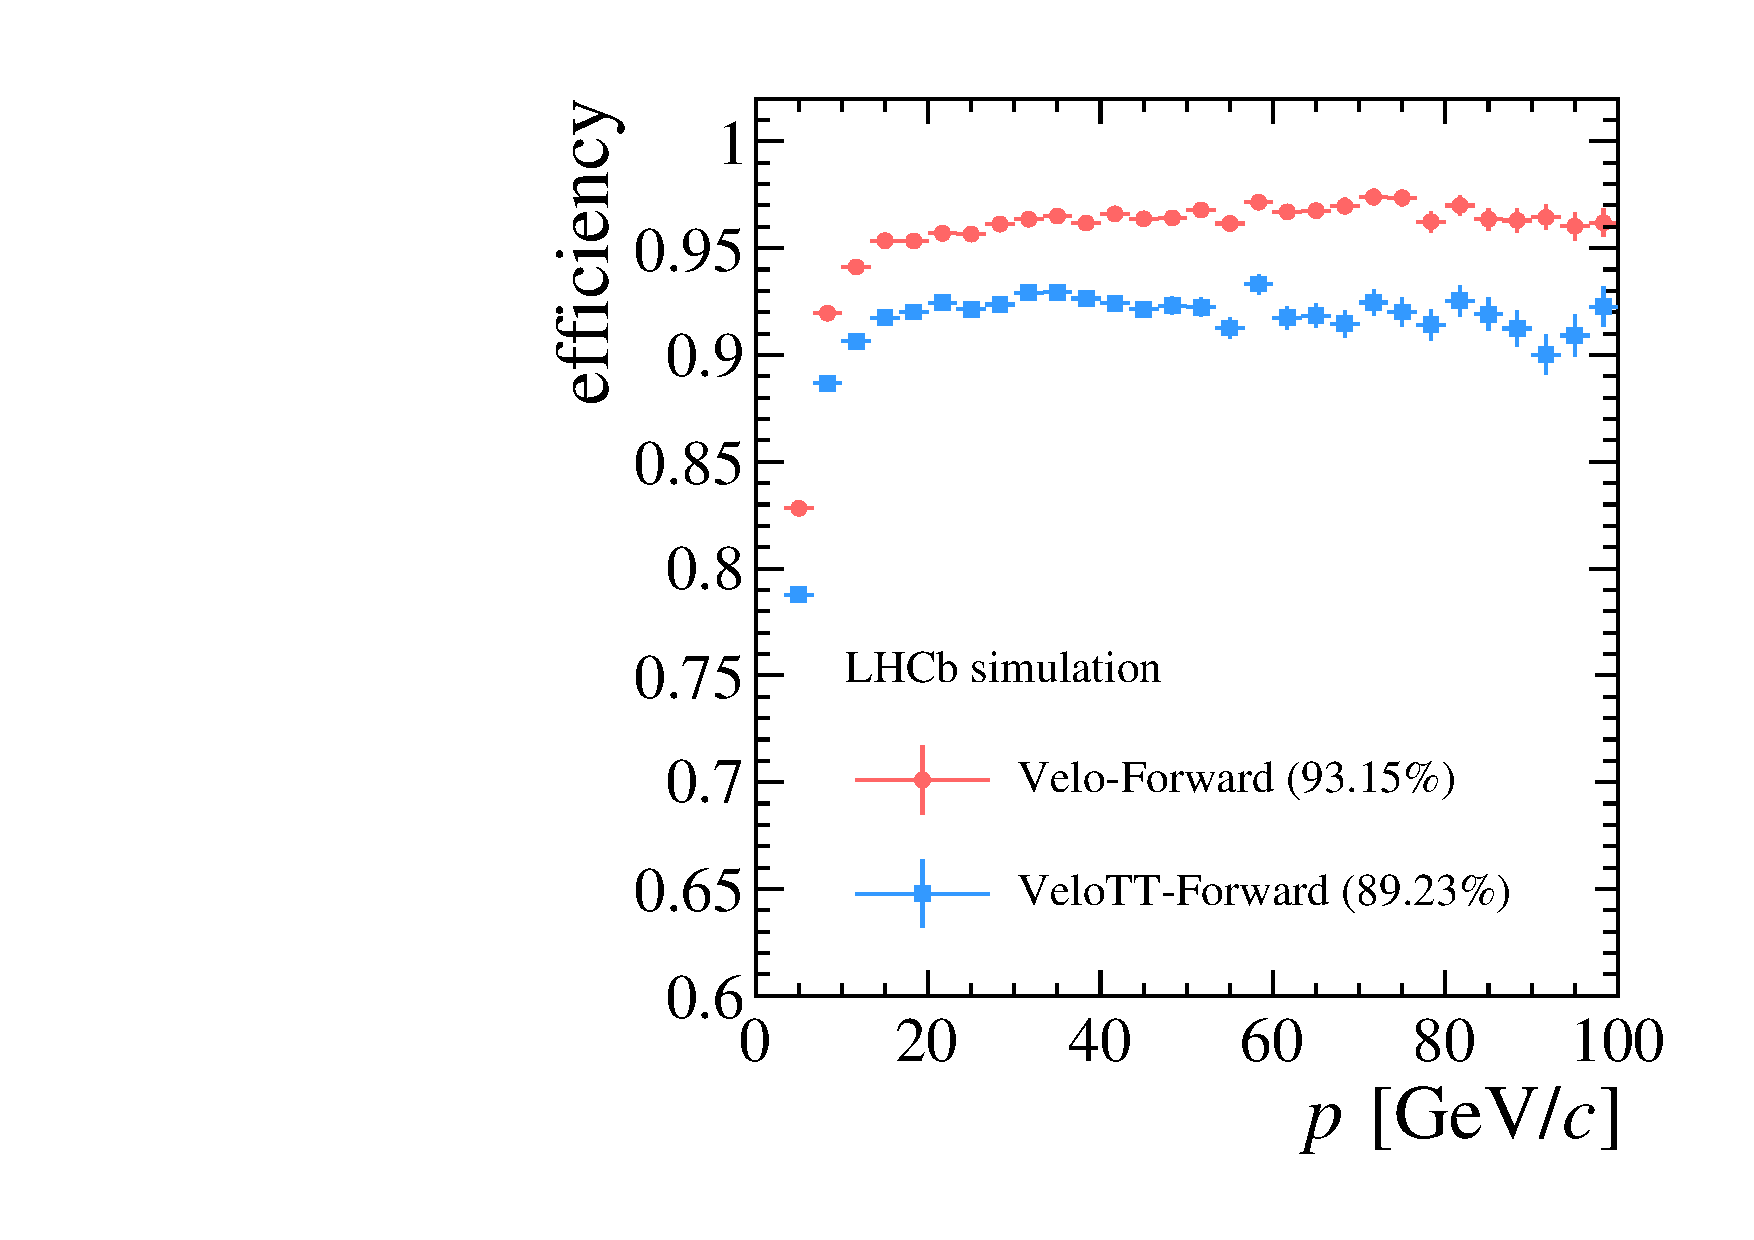
\includegraphics[width=0.45\linewidth]{figs/upstream-tracking-run2/Forward-eff-p.pdf}
    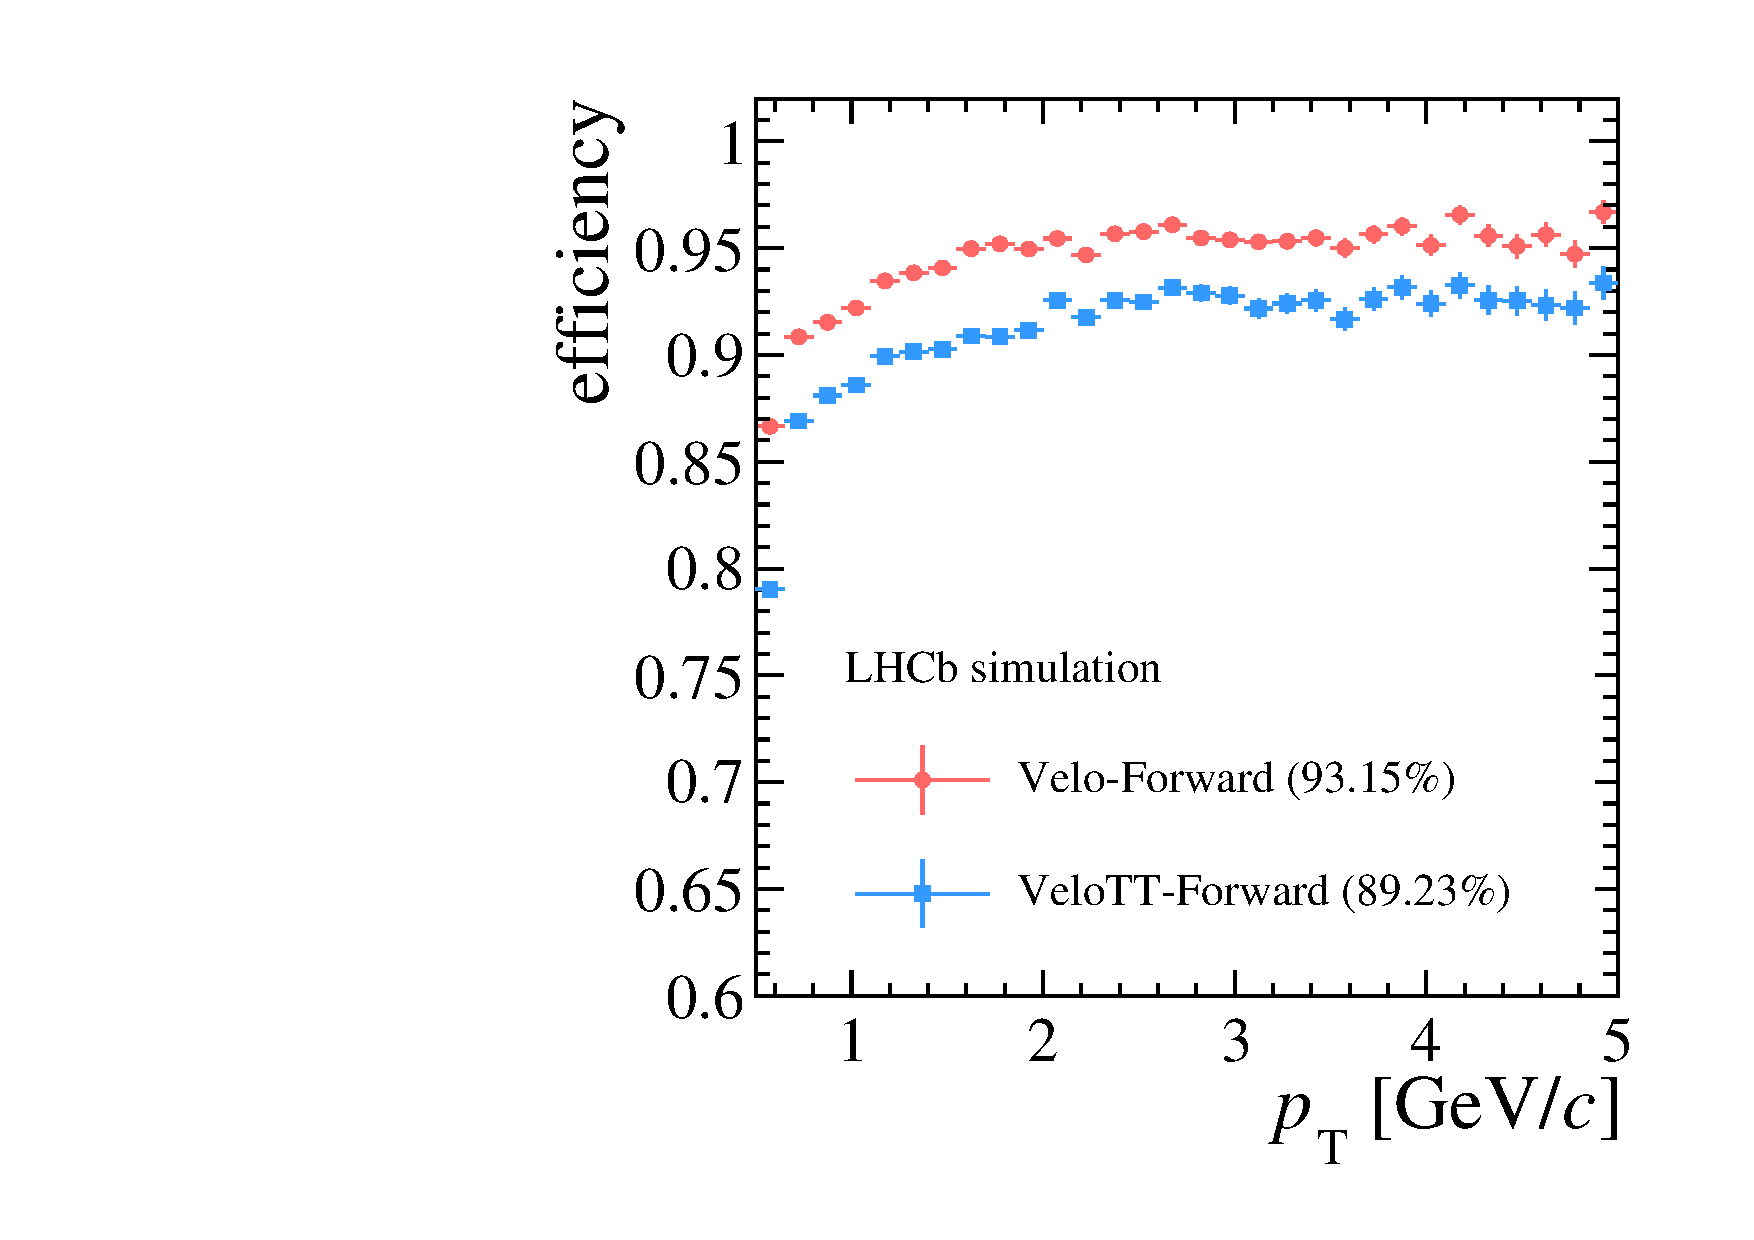
\includegraphics[width=0.45\linewidth]{figs/upstream-tracking-run2/Forward-eff-pt.pdf}
    \caption{The track reconstruction efficiency of the Forward algorithm using \velo or VeloTT tracks as a function of \ptot and \pt.}
    \label{fig:eff_forward_run2_comp}
  \end{center}
\end{figure}

\begin{figure}[!tb]
  \begin{center}
    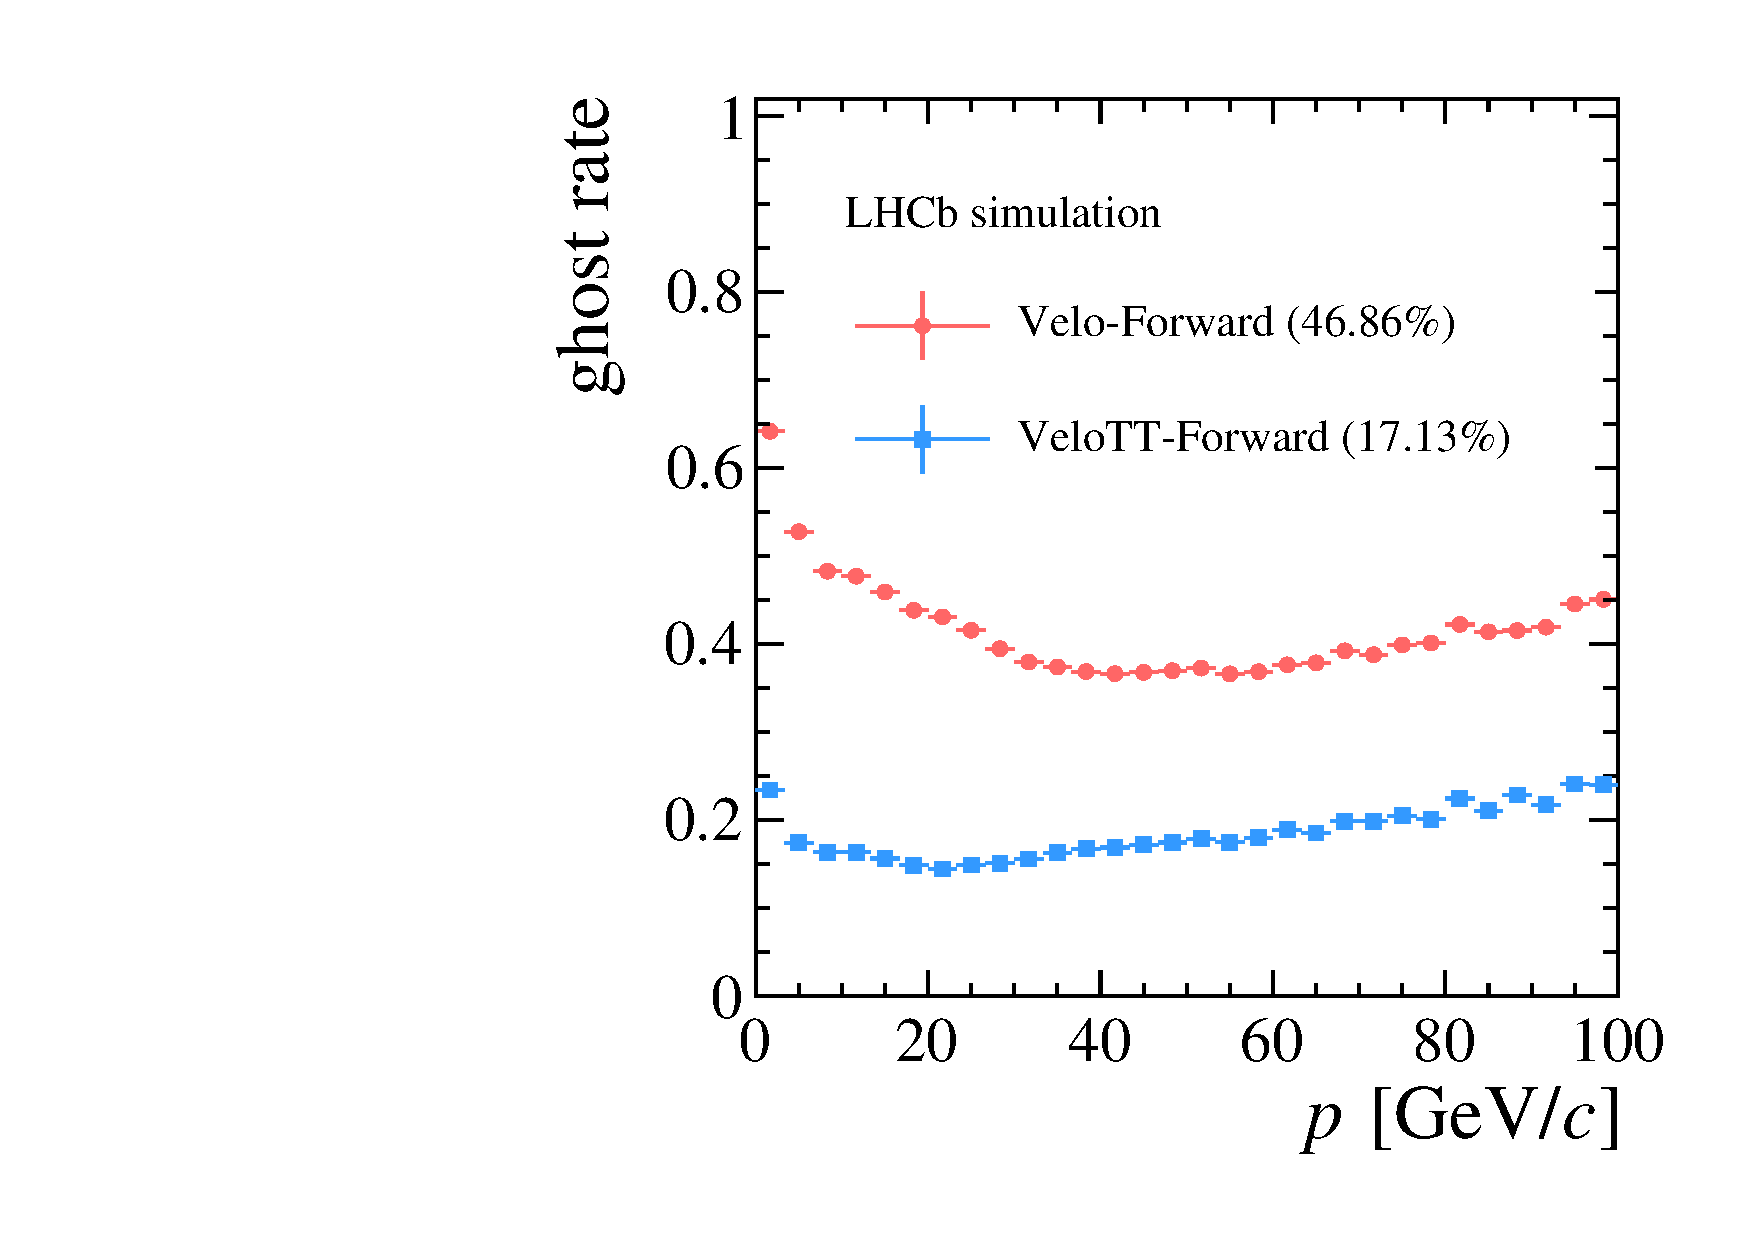
\includegraphics[width=0.45\linewidth]{figs/upstream-tracking-run2/Forward-gr-p.pdf}
    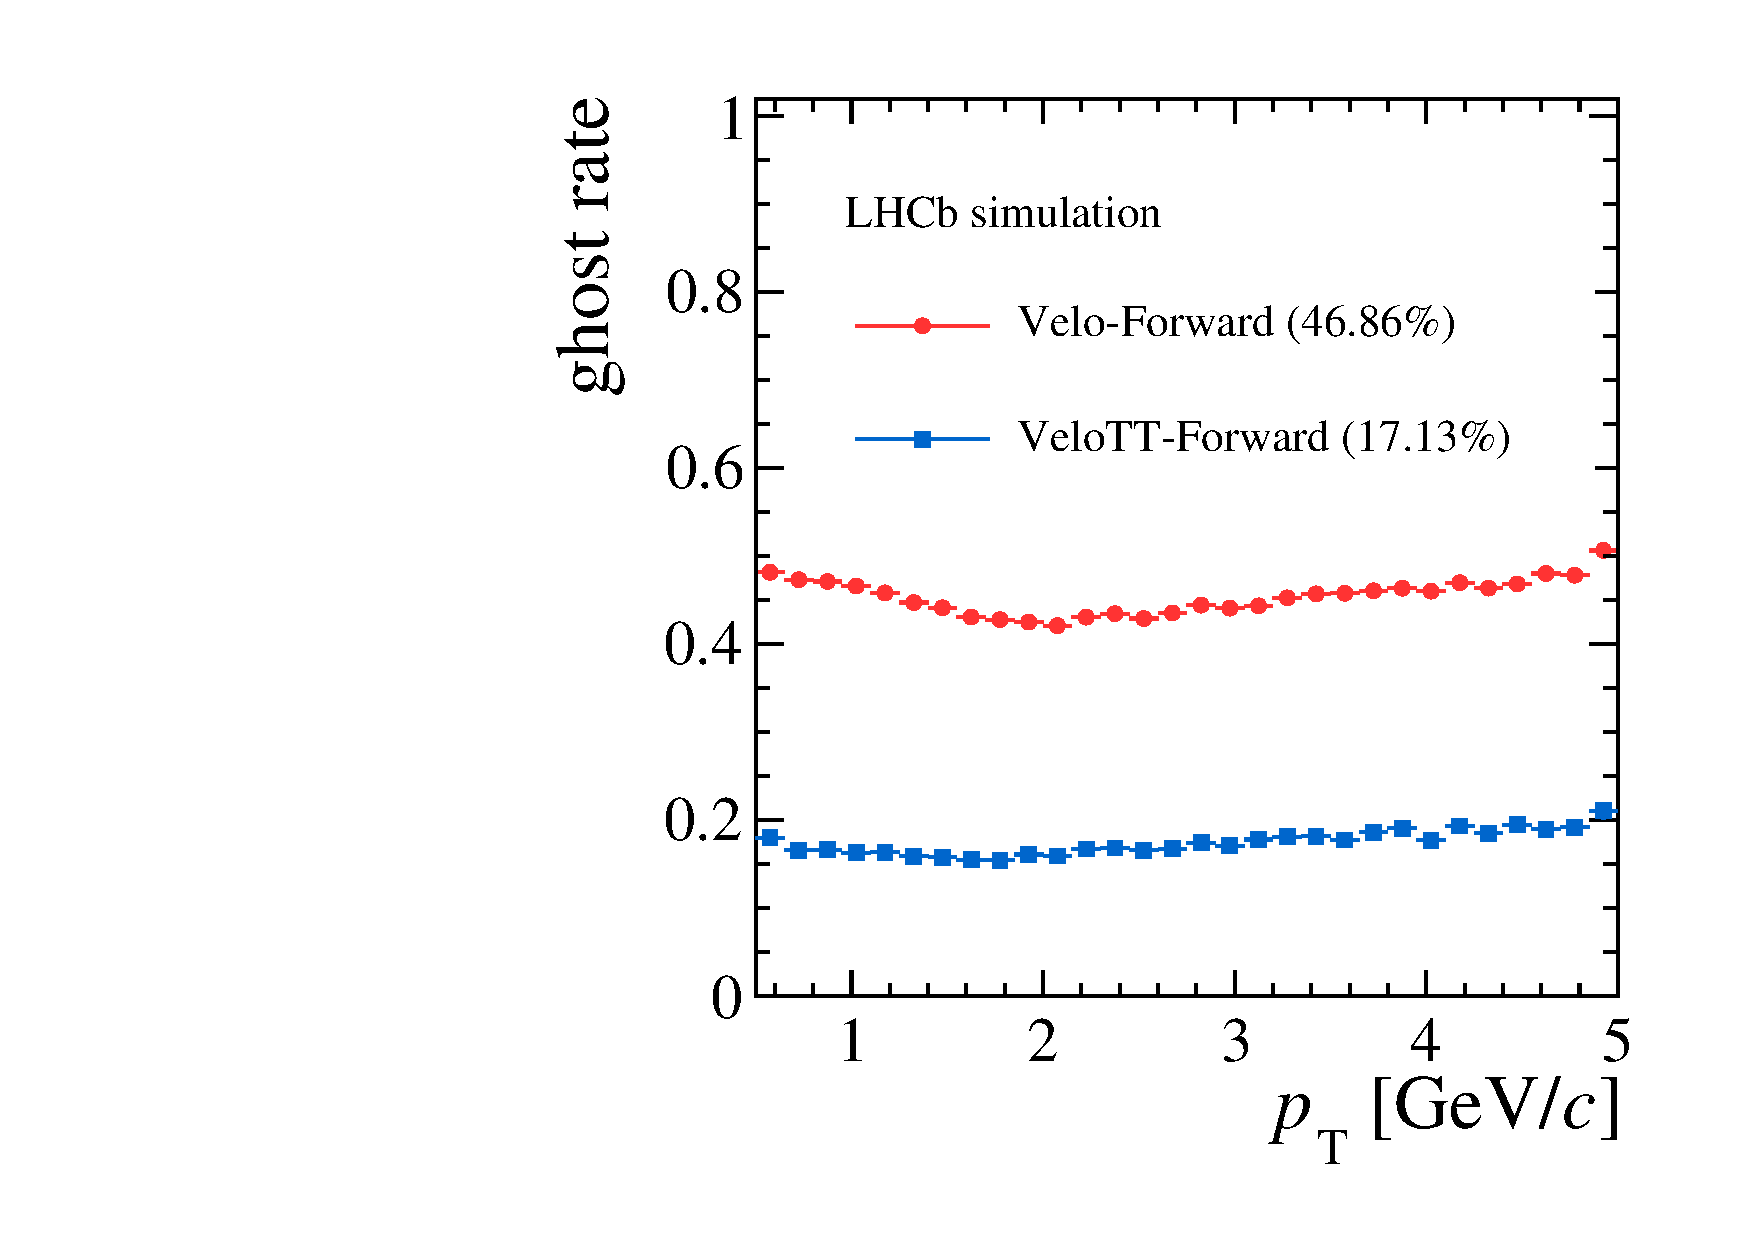
\includegraphics[width=0.45\linewidth]{figs/upstream-tracking-run2/Forward-gr-pt.pdf}
    \caption{The ghost rate of the Forward algorithm using Velo or VeloTT tracks as a function of \ptot and \pt.}
    \label{fig:gr_forward_run2_comp}
  \end{center}
\end{figure}

\subsection{Summary}
\label{sec:up-track-run2:summary}

The improved performance obtained by introducing the VeloTT algorithm into the reconstruction chain in Run II result in two important improvements. Firstly, it is possible to remove any IP requirement on \velo tracks and to loosen the \pt threshold of the Forward tracking from 1.2\gevc to 0.5\gevc in the first stage of the software trigger. This greatly improves the signal efficiency for charm physics and allows lifetime unbiased triggers for hadronic final states for the first time~\cite{hlt-runII}. Secondly, significant improvements to the reconstruction sequence in the second stage of the software trigger have allowed the convergence of the online and offline reconstruction. Combined with a novel approach providing real-time alignment and calibration~\cite{alignment}, this allows physics analyses to be performed directly on the output of the software trigger~\cite{turbo}. Only writing out the information of the signal candidates leads to a large saving in storage space ($\sim 90$\%). This is ideal for the analysis of channels with high yields that would previously have been heavily pre-scaled. It also allows rapid turn-around from data taking to analysis on the order of a few weeks~\cite{jpsi-em,charm-em}.

\clearpage
\section{Differential branching fraction and angular analysis of \mbox{\BdToKpimm} decays}
\label{sec:kpimm}

\subsection{Introduction}

\label{sec:kpimm:introduction}

The decay \BdToKpimm is a flavour-changing neutral-current process. In the Standard Model (SM), the leading order transition amplitudes are described by electroweak penguin or box diagrams.  In extensions to the SM, new heavy particles can contribute to loop diagrams and modify observables such as branching fractions and angular distributions.

\subsubsection[Previous \btosmm measurements]{Previous \boldmath{\btosmm} measurements}
The previous angular analyses of \BdToKpimm performed by the \lhcb collaboration~\cite{LHCB-PAPER-2011-020,LHCB-PAPER-2013-019,LHCB-PAPER-2013-037,LHCB-PAPER-2015-051} focused on the $K^{+}\pi^{-}$ invariant mass range $796<\mkpi<996\mevcc$ where the decay proceeds predominantly via the P-wave process $\decay{\Kstar(892)^{0}}{\kpi}$. A global analysis of the \CP-averaged angular observables measured in the \lhcb Run 1 data sample indicated differences with SM predictions at the level of 3.4 standard deviations~\cite{LHCB-PAPER-2015-051}. The results of the measurement of the observable $P_{5}^{'}$, which exhibits a local deviation from the SM predictions, is shown in Fig.~\ref{fig:kpimm:p5prime}.

\begin{figure}[!b]
\centering
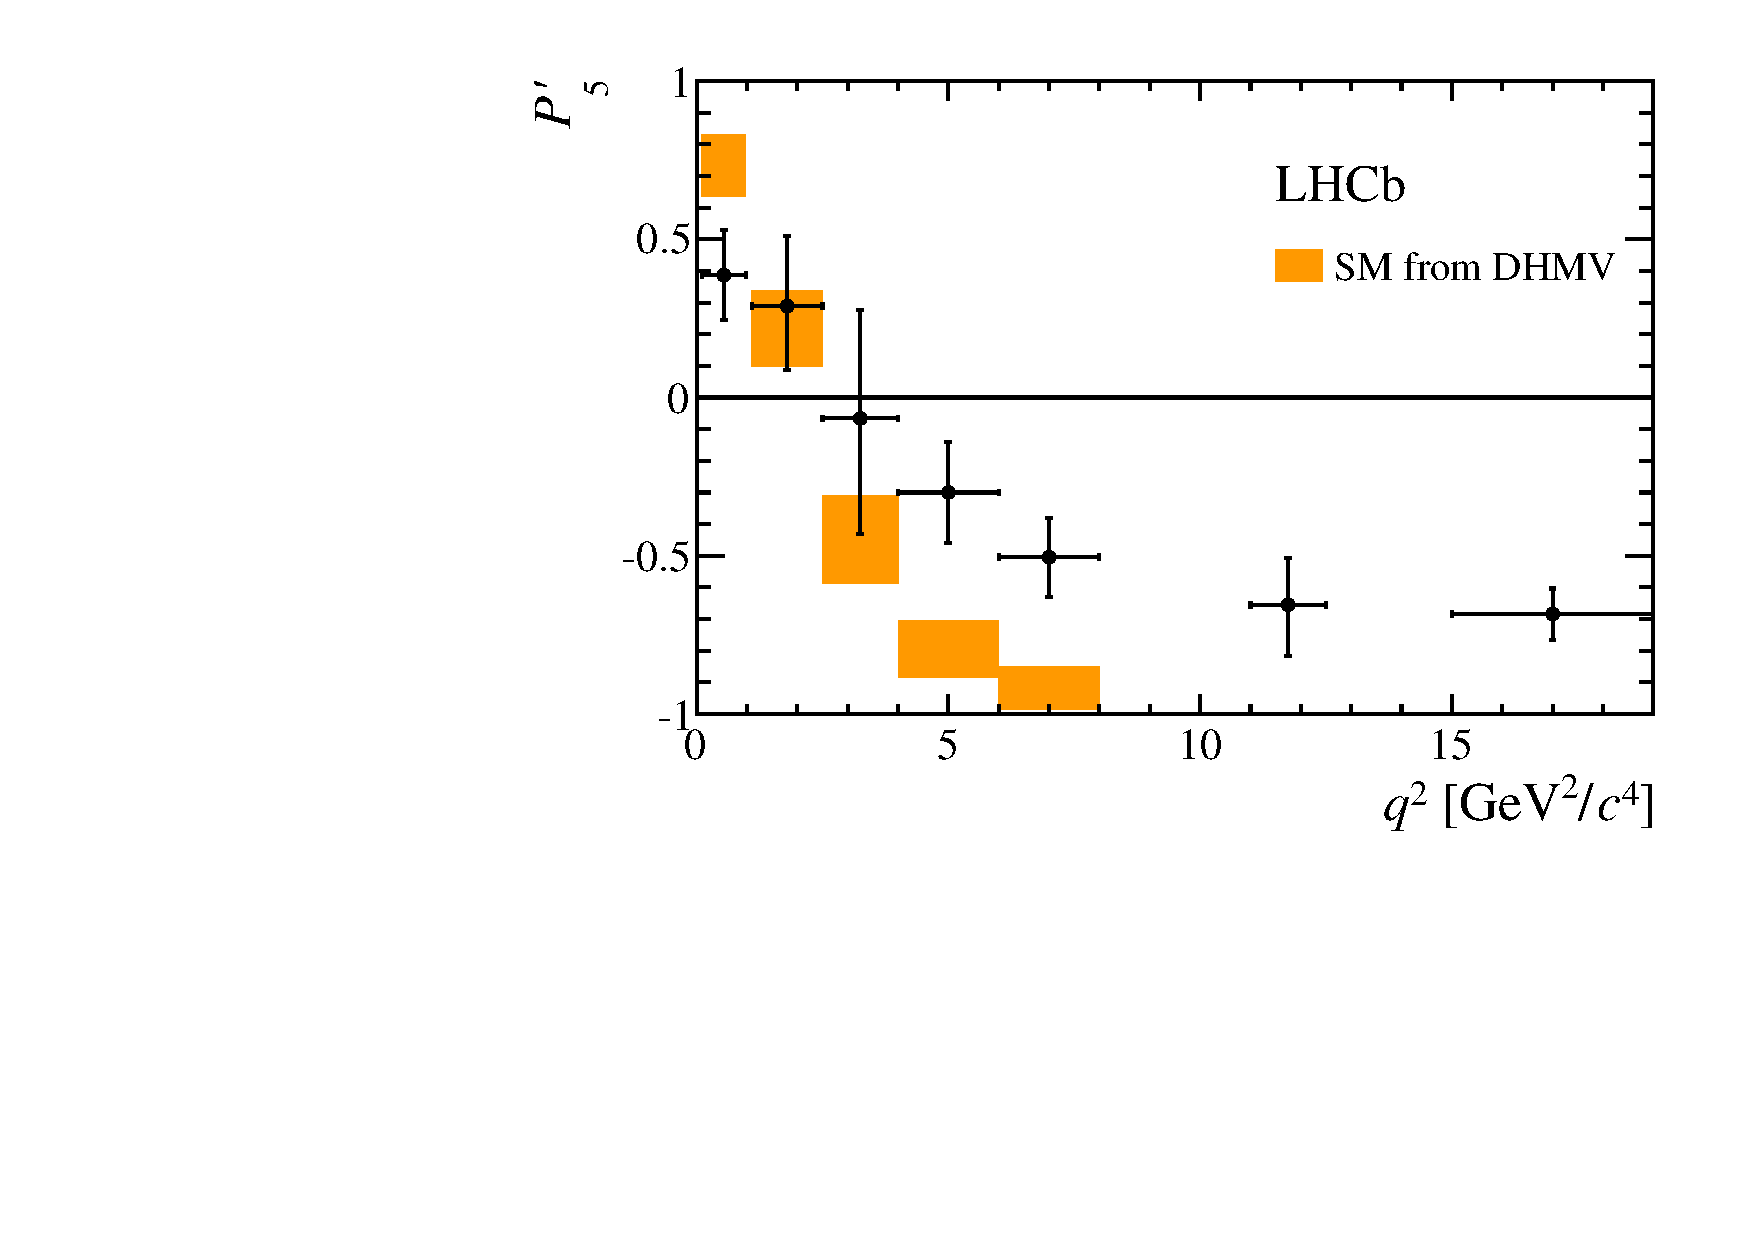
\includegraphics[width=0.7\textwidth]{figs/kpimm/introduction/P5prime.pdf}
\caption{Results of the measurement of the observable $P_{5}^{'}$ by the \lhcb collaboration. The SM predictions are taken from Ref.~\cite{pprime-theory}.}
\label{fig:kpimm:p5prime}
\end{figure}

This set of measurements is part of a pattern of discrepancies with respect to SM predictions that have been observed in \btosmm transitions. For example, the measured differential branching fractions of the decays \BsTophimm~\cite{LHCB-PAPER-2015-023}, $\decay{\Lb}{\Lambda\mumu}$~\cite{LHCB-PAPER-2015-009} and \BuToKmm~\cite{LHCB-PAPER-2014-006} all lie below their corresponding SM predictions. Furthermore, the ratio $R_{K} = \BF(\decay{\Bp}{\Kp\mup\mun})/\BF(\decay{\Bp}{\Kp\ep\en})$, which is a test of lepton flavour universality, was also measured to be 2.6 standard deviations from its SM prediction of unity~\cite{LHCB-PAPER-2014-024}.

This pattern of discrepancies can be intepreted by performing global model-independent fits to \btosmm measurements~\cite{Altmannshofer:2015sma}.{\interfootnotelinepenalty=10000\footnote{The global fit in Ref.~\cite{Altmannshofer:2015sma} takes into account 88 measurements of 76 observables by the \atlas, \babar, \belle, \cdf, \cms and \lhcb experiments.}} In the framework of OPE, described in Sec~\ref{sec:theory:rare}, these fits can be used to constrain the values of the Wilson coefficients $\mathcal{C}_{7}$, $\mathcal{C}_{9}$ and $\mathcal{C}_{10}$. A $\chi^{2}$ function which quantifies the compatibility of the model with the data, for a given set of values of the Wilson coefficients, is minimised in different scenarios. The NP dependencies are encoded as NP contributions to the Wilson coefficients, $\mathcal{C}_{i}^{\rm NP} = \mathcal{C}_{i}-\mathcal{C}_{i}^{\rm SM}$. The best fit is obtained when allowing NP in $\mathcal{C}_{9}$ only, yielding a value of $\mathcal{C}_{9}^{\rm NP} = -1.07$ which correponds to a pull of 3.7 standard deviations from the SM. Figure~\ref{fig:kpimm:c9c10} shows the result of the fit when allowing for NP effects in both $\mathcal{C}_{9}$ and $\mathcal{C}_{10}$. These results are in good agreement with Ref.~\cite{Descotes-Genon:2015uva}, which also finds that a negative contribution to $\mathcal{C}_{9}$ plays a central role in explaining the observed discrepancies.

\begin{figure}[!tb]
\centering
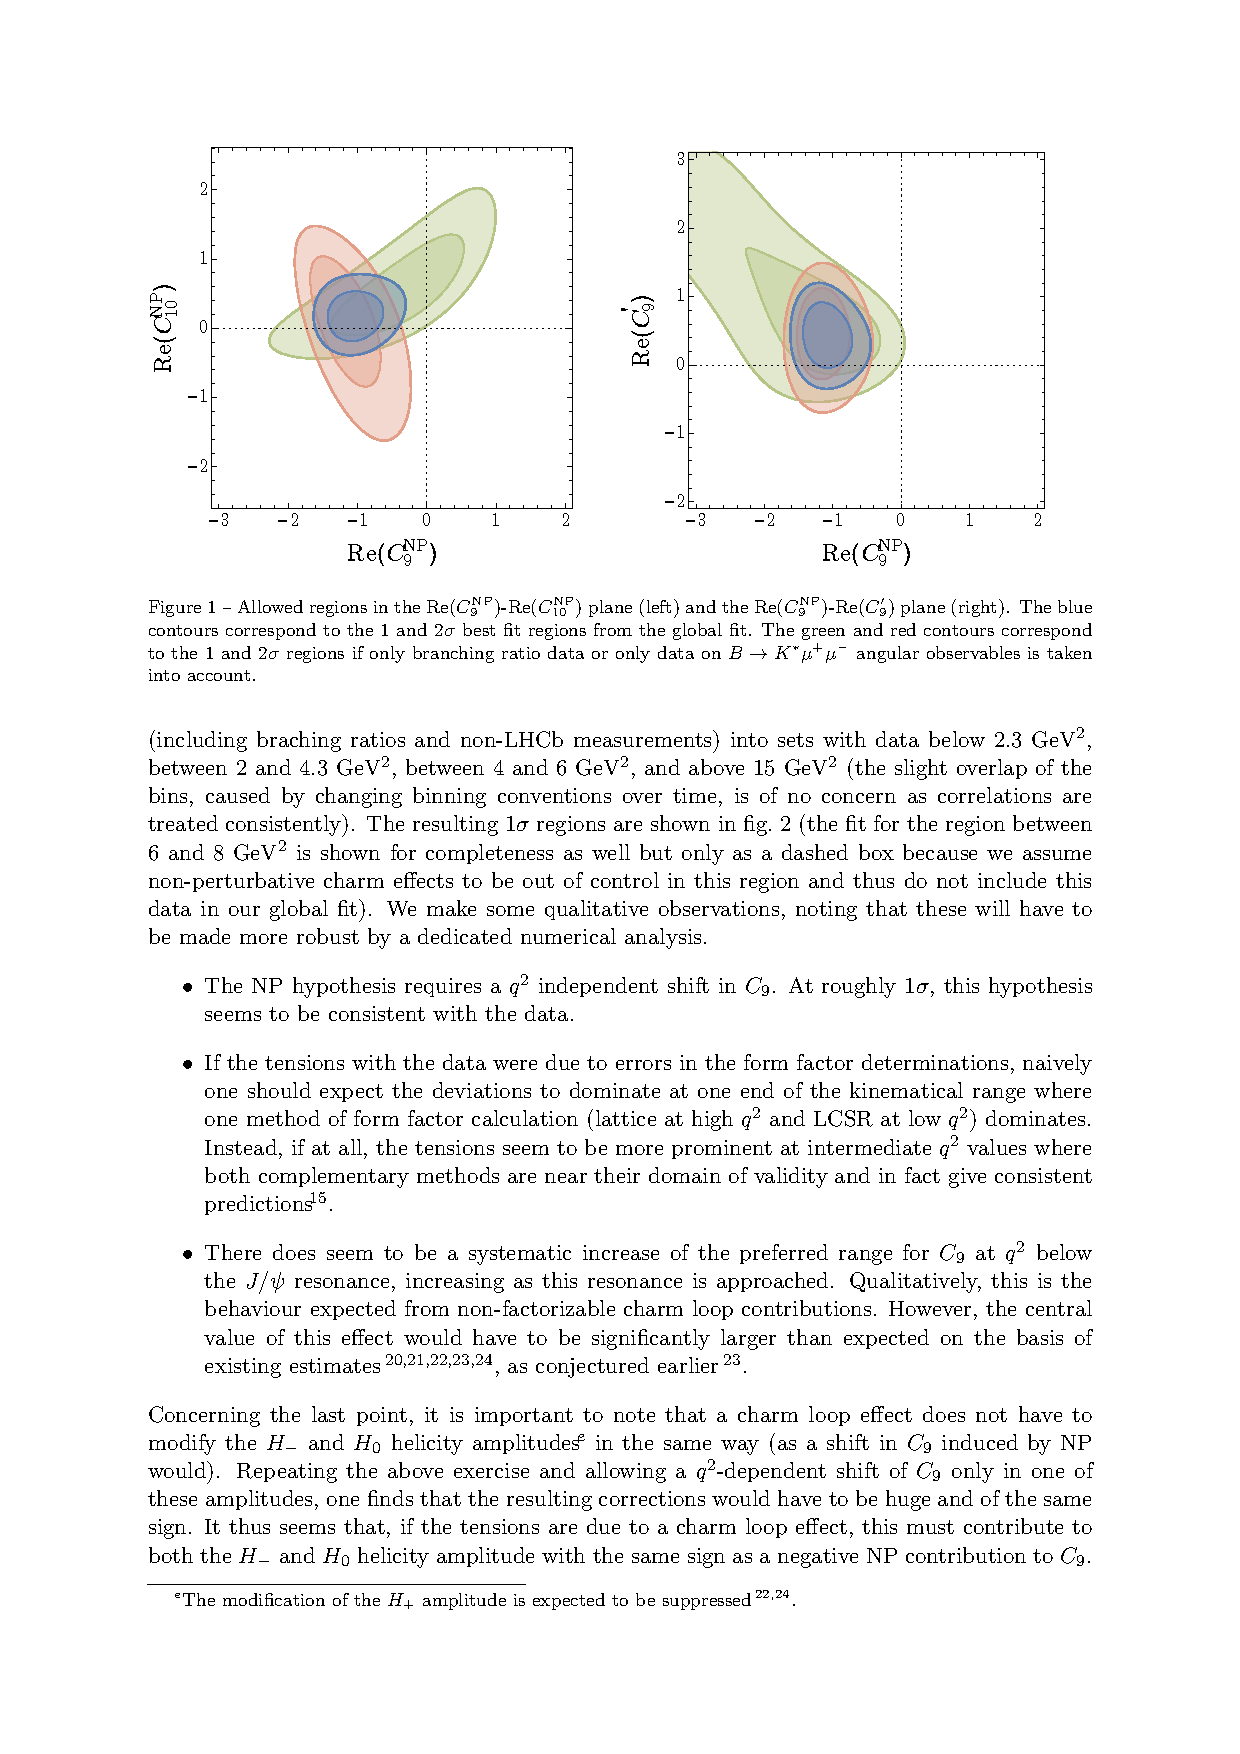
\includegraphics[trim={2.5cm 20cm 10.7cm 2.4cm},clip,width=0.6\textwidth]{figs/kpimm/introduction/c9c10.pdf}
\caption{Allowed region in the ${\rm Re}(\mathcal{C}_{9}^{\rm NP})$--${\rm Re}(\mathcal{C}_{10}^{\rm NP})$ plane. The blue contours correspond to the 1$\sigma$ and 2$\sigma$ best fit regions from the global fit. The red and green contours represent 1$\sigma$ and 2$\sigma$ regions if only the \BdToKstmmP angular observables or only the differential branching fraction measurements are taken into account, respectively. Taken from Ref.~\cite{Altmannshofer:2015sma}.}
\label{fig:kpimm:c9c10}
\end{figure}

Many NP models have been proposed to explain this observed tension from the SM in $\mathcal{C}_{9}$. Such models contain new interactions mediated by a $Z^{'}$ boson~\cite{Gauld:2013qja,Altmannshofer:2014cfa,Crivellin:2015mga} or leptoquarks~\cite{Sahoo:2015wya,Biswas:2014gga,Hiller:2014ula}. These interactions can also introduce a violation of lepton flavour universality.

However, it has also been suggested that the contribution of so-called charm-loop effects could be responsible for the observed deviations~\cite{Lyon:2014hpa}. As these hadronic effects are mediated via virtual photon exchange, leading to a vector-like coupling to leptons, it is possible they could mimic NP effects in $\mathcal{C}_{9}$.

Since short distance effects are universal and should appear coherently in all \btosmm transitions, measuring other \btosmm transitions can help to shed light on this situation.

% \begin{figure}[!tb]
% \centering
% 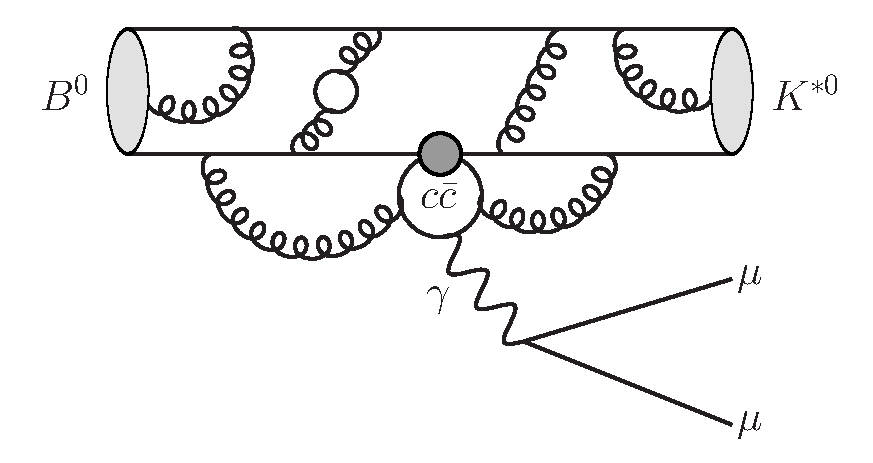
\includegraphics[width=0.6\textwidth]{figs/kpimm/introduction/btosll_charm.eps}
% \caption{}
% \label{fig:kpimm:charm-loops}
% \end{figure}

\subsubsection{Analysis overview}

Since the dominant structures in the \kpi invariant mass spectrum of \BdToKpimm above the P-wave $\Kstar(892)^{0}$ are resonances in the 1430\mevcc region, this is a natural region to study. The relevant \Kstarz states above the \KstP mass range are listed in Table~\ref{tab:introduction:states}. Throughout this paper, the symbol $\Kstarz$ denotes any neutral strange meson in an excited state that decays to a \Kp\pim final state. In the 1430\mevcc region, contributions are expected from the S-wave $K^\ast_0(1430)^0$, P-wave $K^\ast(1410)^0$ and D-wave $K^\ast_2(1430)^0$ states, as well as the broad P-wave $K^\ast(1680)^0$ state. 

\begin{table}[!tb]
\caption{Expected resonant contributions above the \KstP mass range. For each, the spin-parity, $J^P$, and branching fraction to $\kaon\pion$, $\mathcal{B}(K\pi)$, are given. Taken from Ref.~\cite{lu-wang}.}
\label{tab:introduction:states}
\centering
\begin{tabular}{c|c|c|c|r}
    Resonance & $J^{P}$ & Mass [$\mathrm{Me\kern -0.1em V\!/}c^2$] & Full width [$\mathrm{Me\kern -0.1em V\!/}c^2$]  & $\mathcal{B}(K\pi)~[\%]$ \\
   \hline
   $K^\ast(1410)^0$ & $1^{-}$& $\hphantom{0.}1414 \pm 15\hphantom{.}$& $232 \pm 21\hphantom{0}$  & $6.6 \pm 1.3$ \\
   $K^\ast_0(1430)^0$ & $0^{+}$ & $\hphantom{0.}1425 \pm 50\hphantom{.}$ & $270 \pm 80\hphantom{0}$ & $\hphantom{.}93 \pm 10\hphantom{.}$ \\
   $K^\ast_2(1430)^0$ & $2^{+}$ & $1432.4\pm 1.3$ & $109 \pm 5\hphantom{00}$ & $49.9 \pm 1.2$ \\
   $K^\ast(1680)^0$ & $1^{-}$ & $\hphantom{0.}1717 \pm 27\hphantom{.}$ & $322 \pm 110$ & $38.7 \pm 2.5$ \\
   $K^\ast_3(1780)^0$ & $3^{-}$ & $\hphantom{0.}1776 \pm 7\hphantom{0.}$ & $159 \pm 21\hphantom{0}$ & $18.8 \pm 1.0$ \\
   $K^\ast_4(2045)^0$ & $4^{+}$ & $\hphantom{0.}2045 \pm 9\hphantom{0.}$ & $198 \pm 30\hphantom{0}$ & $9.9 \pm 1.2$ \\
 \end{tabular}
 \end{table}

The \mkpi distribution for \BdToKpimm decays in the range $1.1<\qsq<6.0\gevgevcccc$ and $630<\mkpi<1630\mevcc$ is shown in Fig.~\ref{fig:full-mkpi}, where $\qsq \equiv m^2(\mup \mun)$. The candidates are obtained using the selection described in Sec.~\ref{sec:kpimm:selection} and the background component is subtracted using the \sPlot technique~\cite{splot}. The main structures are observed around the mass of the $\Kstar(892)^{0}$ resonance and in the 1430\mevcc region. 

\begin{figure}[!tb]
 \centering
 \includegraphics[width=0.7\linewidth]{figs/kpimm/introduction/full-mkpi.pdf}
 \caption{Background-subtracted \mkpi distribution for \BdToKpimm decays in the range $1.1<\qsq<6.0\gevgevcccc$. The region $1330<\mkpi<1530~\mevcc$ is indicated by the blue hatched area.}
\label{fig:full-mkpi}
\end{figure}

This chapter describes the first measurements of the differential branching fraction and angular moments of \BdToKpimm in the region $1330<\mkpi<1530\mevcc$. The values of the differential branching fraction are reported in five bins of \qsq between 0.1 and 8.0\gevgevcccc, and in the range $1.1<\qsq<6.0\gevgevcccc$ for which the angular moments are also measured. The measurements are based on samples of $pp$ collisions collected by the \lhcb experiment in Run 1, corresponding to integrated luminosities of 1.0\invfb at a centre-of-mass energy of 7\tev and 2.0\invfb at 8\tev.  
\subsection{Angular distribution and observables}
\label{sec:kpimm:angular-distribution}

\begin{figure}
\centering
\begin{subfigure}{0.49\textwidth}
\includegraphics[width=\textwidth]{figs/kpimm/angular-distribution/angles_bzb.pdf}
\caption{}
\label{fig:angle_conventions:bzb}
\end{subfigure}
\begin{subfigure}{0.49\textwidth}
\centering
\includegraphics[width=\textwidth]{figs/kpimm/angular-distribution/angles_bz.pdf}
\caption{}
\label{fig:angle_conventions:bz}
\end{subfigure}
\caption{Angle conventions for the (a) $\Bzb \to \Km \pip \mun \mup$ (b)  $\Bz \to \Kp \pim \mup \mun$ as described in Ref.~\cite{biplab}. The leptonic and hadronic frames are back-to-back with a common $\hat{y}$ axis. For the dihedral angle $\phi$ between the leptonic and hadronic decay planes, there is an additional sign flip $\phi\to -\phi$ compared to previous \lhcb analyses~\cite{LHCB-PAPER-2011-020,LHCB-PAPER-2013-019,LHCB-PAPER-2013-037,LHCB-PAPER-2015-051}.
}
\label{fig:angle_conventions}
\end{figure}

The final state of the decay \BdToKpimm is fully described by five kinematic variables: three decay angles (\thetal, \thetak, $\phi$), \mkpi, and \qsq.
Figure~\ref{fig:angle_conventions:bzb} shows the angle conventions for the $\Bzb$ decay (containing a \bquark quark): the back-to-back leptonic and hadronic systems share a common $\hat{y}$ axis and have opposite $\hat{x}$ and $\hat{z}$ axes.
The negatively charged lepton is used to define the leptonic helicity angle $\thetal$ for the $\Bzb$.
The quadrant of the dihedral angle $\phi$ between the dimuon and the $\Kstarzb \to \Km\pip$ decay planes is determined by requiring the azimuthal angle of the $\mun$ to be zero in the leptonic helicity frame. The azimuthal angle of the $\Km$ in the hadronic helicity frame is then equal to $\phi$. Compared to the dihedral angle used in the previous \lhcb analyses~\cite{LHCB-PAPER-2011-020,LHCB-PAPER-2013-019,LHCB-PAPER-2013-037,LHCB-PAPER-2015-051}, there is a sign flip, $\phi \to -\phi$, in the convention used here. For the $\Bz$ decay (containing a \bquarkbar quark), the charge conjugation is performed explicitly, and the angles are shown in Fig.~\ref{fig:angle_conventions:bzb}, where for the $\Bz$, the $\mup$ and $\Kp$ directions are used to define the angles. An additional minus sign is added to the dihedral angle when performing the \CP conjugation, in order to keep the measured angular observables the same between $\Bzb$ and $\Bz$ in the absence of direct \CP violation.

In the limit where \qsq is large compared to the square of the muon mass, the \CP-averaged differential decay rate of \BdToKpimm with the \Kp\pim system in a S-, P-, or D-wave configuration can be expanded in an orthonormal basis of angular functions $f_i(\Omega)$ as

\begin{equation}
\label{eqn:vector_moments}
\frac{\deriv\Gamma }{\deriv\qsq\,\deriv\Omega} \propto \sum^{41}_{i=1} f_i (\Omega) \Gamma_i(\qsq)
 \quad\mbox{with}\quad
\Gamma_i(\qsq) = \Gamma^L_i(\qsq) + \eta^{L\to R}_i\; \Gamma^R_i(\qsq),
\end{equation}

\noindent where $\deriv\Omega = \deriv\!\ctl\,\deriv\!\ctk\,\deriv\phi$, and $L$ and $R$ denote the (left- and right-handed) chirality of the lepton system~\cite{biplab}. The sign $\eta^{L\to R}_i=\pm 1$ depends on whether $f_i$ changes sign under $\thetal \to \pi + \thetal$. 
\noindent The orthonormal angular basis is constructed out of spherical harmonics, \mbox{$Y^m_l \equiv Y^m_l (\thetal,\phi)$}, and reduced spherical harmonics, \mbox{${P^m_l \equiv \sqrt{2 \pi}Y^m_l(\thetak,0)}$}.
 
The transversity-basis moments of the 41 orthonormal angular functions are given in Appendix~\ref{sec:appendix:angular-distribution}. The convention is that the amplitudes correspond to the $\Bzb$ decay. The S-, P- and D-wave transversity amplitudes are denoted as $S^{\{L,R\}}$, $H^{\{L,R\}}_{\{0,\parallel,\perp\}}$ and $D^{\{L,R\}}_{\{0,\parallel,\perp\}}$, respectively. 

The measured angular observables are averaged over the range $1330<\mkpi<1530~\mevcc$ and $1.1<\qsq<6.0\gevgevcccc$. This \qsq range is part of the large-recoil regime where the recoiling \Kstarz has a relatively large energy, $E_{\Kstarz}$, as measured in the rest frame of the parent \B meson. In the limit $\Lambda_{\rm QCD}/E_{\Kstarz} \to 0$, the uncertainties arising from hadronic effects in the relevant form-factors are reduced at leading order, resulting in more reliable theory predictions~\cite{DescotesGenon:2013wba}. The high-$\qsq$ region above the $\psi(2S)$ resonance is polluted by broad charmonium resonances and is also phase-space suppressed for higher \mkpi masses. Therefore, that region is not considered in this study.

In the present analysis, the first moment, $\Gamma_{1}(\qsq)$, corresponds to the total decay rate. From this, 40 normalised moments for $i \in \{2,...,41\}$ are defined as
\begin{equation}
\label{eqn:norm_mom_def}
\overline{\Gamma}_i(\qsq) = \frac{\Gamma_{i}(\qsq)}{\Gamma_{1}(\qsq)}.
\end{equation}
\noindent These form the set of observables that are measured in the angular moments analysis described in Sec.~\ref{sec:kpimm:angular-analysis}.
\subsection{Candidate selection}
\label{sec:kpimm:selection}

The selection of \BdToKpimm candidates comprises several steps. Firstly, candidates are required to have `fired' at least one of the specified trigger lines at each of the three stages of the trigger. Subsequently, candidates must pass two sets of requirements: the first is a common selection known as `stripping' and the second is a loose preselection. Next, combinatorial background candidates are reduced using a multivariate classifier. Finally, exclusive backgrounds are removed with specific vetoes.

\subsubsection{Data samples}

The Run 1 data sample collected by the \lhcb experiment is used for this analysis, corresponding to an integrated luminosity of 3.0\invfb. The data were recorded in \proton\proton collisions at centre-of-mass energies of 7 and 8\tev during 2011 and 2012, respectively. In addition, a number of simulated samples are used to evaluate possible peaking background contributions and to determine the acceptance correction.

\subsubsection{Trigger requirements}

At the first stage of the trigger, \lone, the event must have been triggered by a single muon from the \BdToKpimm decay. At the second level of the trigger, \hltone, at least one of two possible trigger lines must have been triggered by a single daughter particle from the \BdToKpimm decay. At the final level of the trigger, \hlttwo, at least one of several trigger lines must have been triggered by the daughters of the \BdToKpimm decay: these include both topological and muon triggers.

\subsubsection{Stripping and preselection}

The stripping is a set of common, cut-based requirements used to loosely select candidates of interest for similar analyses. The stripping line used in this analysis selects candidates of the form $\decay{\B}{X\mumu}$, where $X$ is one or more hadrons. The full set of stripping requirements are shown in Table~\ref{table:stripping}. The boolean variable \texttt{IsMuon} is used to select muons and requires the particle to have left hits in a given number of muon stations depending on its measured momentum. A global event cut (GEC) is applied on the number of hits in the SPD to reject very high multiplicity events. 

\begin{table}[!tb]
  \centering
  \caption{Stripping requirements applied to \BdToKpimm candidates.}
  \label{table:stripping}
    \begin{tabular}{l|c}
     & Requirement \\
    \hline
    \multirow{5}{*}{\B} & $4600<M< 7000\mevcc$ \\
    & vertex quality $\chi^{2}/{\rm ndf} < 6$ \\
    & vertex separation $\chi^{2} > 121$  \\
    & IP $\chi^{2} < 16$ \\
    & DIRA $< 14\mrad$  \\
    \hline
    \multirow{3}{*}{\Kstarz} & $M < 6200\mevcc$ \\
    & vertex quality $\chi^{2}/{\rm ndf} < 12$ \\
    & vertex separation $\chi^{2} > 9$  \\
    \hline
    \multirow{2}{*}{\mumu} &  $M < 7100\mevcc$ \\
    & vertex quality $\chi^{2}/{\rm ndf} < 12$ \\
    \hline
    \multirow{2}{*}{$\mu$} & \texttt{IsMuon} \\
    & \dllmupi $>$ -3 \\
    \hline
    \multirow{2}{*}{tracks} & Ghost probability $< 0.4$ \\
    & IP $\chi^{2} > 9$  \\
    \hline
    GEC & SPD multiplicity $< 600$ \\
 \end{tabular}
\end{table}

A loose preselection of candidates is performed to remove pathological events. The full set of preselection requirements are shown in Table~\ref{table:presel}. The boolean variable \texttt{hasRich} requires the particle to have information from the \rich detectors. The angles $\theta$ and $\theta_{\rm pair}$ represent the opening angle of a track from the beam and the opening angle between a track pair, respectively. The variables $\langle X \rangle$, $\langle Y \rangle$ and $\langle Z \rangle$ denote the mean primary vertex position.

\begin{table}[!tb]
  \centering
  \caption{Preselection requirements applied to \BdToKpimm candidates.}
  \label{table:presel}
  \begin{tabular}{l|c}
    & Requirement \\
    \hline
    \multirow{2}{*}{\kaon} & \texttt{hasRich} \\
    & \dllkpi~$>$~-5 \\
    \hline
    \multirow{2}{*}{\pion} & \texttt{hasRich} \\
    & \dllkpi~$<$~25 \\
    \hline
    track & $0 < \theta < 400$\mrad \\
    track pairs & $\theta_{\rm pair} > 1$\mrad \\
    \hline
    \multirow{3}{*}{PV} & $|X - \langle X \rangle| < \hphantom{20}5\mm$\\
    & $|Y - \langle Y \rangle| < \hphantom{20}5\mm$\\
    & $|Z - \langle Z \rangle| < 200\mm$\\
 \end{tabular}
\end{table}

\subsubsection{Multivariate classifier}

A multivariate classifier is used to reduce the level of combinatorial background. A Boosted Decision Tree (BDT) classifier~\cite{bdt}, with the Adaboost algorithm~\cite{adaboost} is employed. The BDT was originally developed for the angular analysis of \BdToKstmm~\cite{kstmm-3fb}. 

The BDT uses a combination of kinematic and PID input variables: the \Bz candidate lifetime, the \Bz \ptot and \pt, the \Bz DIRA, the \Bz vertex quality $\chi^{2}$, the \dllkpi of the kaon and pion, the \dllmupi of the muons and the isolation of the four final state particles. The isolation exploits the idea that the daughters of `true' \BdToKpimm candidates should better isolated from other tracks in the event than those from `fake' candidates. 

The training uses \BdToJPsiKst candidates as a proxy for the signal and \BdToKstmm candidates from the upper mass sideband as a proxy for the background. A $k$-folding approach~\cite{kfold} is employed to allow the full dataset to be used for testing and training in an unbiased way. 

\subsubsection{Exclusive backgrounds}
\label{sec:selection:exclusive}

Several additional requirements are applied to remove contributions from decay modes that will peak at, or near to, the signal peak and therefore distort the distributions of \ctl, \ctk and $\phi$. These decay modes include \LbTopKmm and \BuToKmm as well as misidentified \BdToJPsiKpi, \BdToPsitwosKpi and \BdToKpimm. The full set of requirements are presented in Table~\ref{table:peaking}. These requirements reduce the expected contamination from exclusive background candidates to the level of 2\% of the signal yield,

A background from \LbTopKmm decays arises when the \proton is reconstructed as either of the hadron candidates. Candidates are rejected using PID information and alternative mass hypotheses. For the case when the \proton is reconstructed as the \pion, a new mass is constructed where the \pion is given the \proton mass hypothesis. Likewise for the case when the \proton is reconstructed as the \kaon, a new mass is constructed where the \kaon is given the \proton mass hypothesis, and the \pion the \kaon mass hypothesis. These new mass hypotheses are denoted as \mSwappKmm and \mDoubleSwappKmm repectively. Candidates from \LbTopKmm decays are expected have \mSwappKmm or \mDoubleSwappKmm consistent with the known \Lb mass.

A further peaking background contribution can be formed if a \pim from elsewhere in the event is added to a genuine \BuToKmm decay to form a four-track final state.  As \BuToKmm candidates will accumulate at the nominal \Bp mass, these candidates are expected to reside in the upper \mkpimm sideband. They should also have a \Kp\mumu invariant mass, \mkmm, consistent with the nominal \Bp mass. 

Candidates from \BdToJPsiKpi and  \BdToPsitwosKpi decays can contribute a background if the \pim (\Kp) is misidentified as a \mun (\mup) and the \mun (\mup) is misidentified as a \pim (\Kp).  For the case of $\mun \leftrightarrow \pim$ swaps, the invariant mass of the \pim and the \mup, after assigning the \pim the \muon mass hypothesis, should be consistent with the known \jpsi or \psitwos masses.  Likewise, for the case of $\Kp \leftrightarrow \pip$ swaps, the invariant mass of the \Kp and the \mun, after assigning the \Kp the \muon mass hypothesis, should be consistent with the known \jpsi or \psitwos masses. These new mass hypotheses are denoted $m_{(\pi\to\mu)\mu}$ and $m_{(K\to\mu)\mu}$ respectively.

A background contribution from genuine \BdToKpimm decays can also be formed when the two hadron hypotheses are swapped. This leads to \Bz candidates being incorrectly reconstructed as \Bzb candidates and vice versa. These candidates are vetoed using hadron identification criteria.

\begin{table}[!tb]
  \centering
  \caption{Requirements applied to veto exclusive backgrounds.  All invariant masses have the units \mevcc.}
  \label{table:peaking}
  \makebox[\textwidth][c]{
  \bgroup
    \def\arraystretch{1.5}
  \begin{tabular}{l|l|l}
    Decay mode & Mis-id & Veto\\
    \hline
    \multirow{2}{*}{\LbTopKmm} & $\proton\rightarrow\pion$ & $5575 < \mSwappKmm < 5665 ~ {\rm and} ~ \pion\dllppi > 0$ \\
    & $\proton,\kaon\rightarrow\kaon,\pion$ & $5575 < \mDoubleSwappKmm < 5665 ~  {\rm and}  ~  \pion\dllkpi > 0$\\
    \BuToKmm & Random \pion & $m_{\kaon\pion\muon\muon}>5380 ~ {\rm and} ~ 5220<\mkmm<5340$ \\
    \multirow{2}{*}{\BdToJPsiKpi} & $\pion\leftrightarrow\muon$ & $2996 < m_{(\pion\to\mu)\mu} < 3196 ~ {\rm and} ~ (\pion\texttt{IsMuon} ~{\rm or}~ \pion\dllmupi>0)$ \\
    & $\kaon\leftrightarrow\muon$ & $2996 < m_{(\kaon\to\mu)\mu} < 3196 ~ {\rm and} ~ (\kaon\texttt{IsMuon} ~{\rm or}~ \kaon\dllmupi>0)$\\
    \multirow{2}{*}{\BdToPsitwosKpi} & $\pion\leftrightarrow\muon$ & $3626 < m_{(\pion\to\mu)\mu} < 3746 ~ {\rm and} ~ (\pion\texttt{IsMuon} ~{\rm or}~ \pion\dllmupi>5)$ \\
    & $\kaon\leftrightarrow\muon$ & $3626 < m_{(\kaon\to\mu)\mu} < 3746 ~ {\rm and} ~ (\kaon\texttt{IsMuon} ~{\rm or}~ \kaon\dllmupi>5)$\\
    \BdToKpimm & $\kaon\leftrightarrow\pion$ & $(\kaon\dllkpi - \pion\dllkpi) > 10$ \\
 \end{tabular}
 \egroup
 }
 \end{table}


\subsection{Agreement between data and simulation}
\label{sec:kpimm:data-mc}

Good agreement between data and simulated candidates is necessary in order to be able to accurately model the distortion of the angular distributions caused by the trigger, reconstruction and selection. The acceptance correction, described in detail in Sec.~\ref{sec:kpimm:acceptance}, is determined from simulated four-body \BdToKpimm decays generated according to a phase space distribution. Data driven techniques are used to improve the agreement between data and simulation. The PID distributions in simulation are corrected using a method known as `resampling'. To take into account remaining differences, simulated candidates are reweighted to match specific distributions in data.

\subsubsection{PID resampling}
\label{sec:kpimm:data-mc:resample}

Particle indentification information is used in two places within the selection of \BdToKpimm, for example to veto peaking backgrounds and as input to the multivariate classifier. The PID distributions are known to disagree between data and simulation. In order to improve the agreement, the distributions for each PID variable is resampled in a two stage process. Firstly, histograms of the PID variables are produced in bins of the number of tracks in the event, pseudorapidity and \pt using calibration samples in data. These samples include $\decay{\Dstarp}{\Dz(\to\Km\pip)\pim}$, $\decay{\Lz}{\proton\pim}$ and $\decay{\jpsi}{\mumu}$ decays. Secondly, the PID variables for simulated candidates are updated using the corresponding histogram as a PDF to draw a new value. This sampled value replaces the PID variable for the simulated candidate and is used in subsequent operations. The validation of the method for the variables \kaon\dllkpi and \pion\dllkpi is shown in Fig.~\ref{fig:kpimm:data-mc:pid} using sWeighted\footnote{A description of the \sPlot technique can be found in Ref.~\cite{splot}.} \BdToJPsiKst candidates in data and simulated \BdToJPsiKst candidates. The distributions for the remaining PID variables used in the candidate selection are shown in Appendix~\ref{sec:appendix:data-mc:pid}.

\begin{figure}[!tb]
 \centering
 \includegraphics[width=0.49\textwidth]{figs/kpimm/data-mc/resampling/K_PIDK.pdf}
 \includegraphics[width=0.49\textwidth]{figs/kpimm/data-mc/resampling/Pi_PIDK.pdf}
 \caption{Data-simulation agreement for the PID variables used in the selection of \BdToKpimm. The black data points show the distributions for sWeighted \BdToJPsiKst candidates in data. The red dashed histograms show the nominal distribution for simulated \BdToJPsiKst candidates. The blue histograms show the distribution for simulated \BdToJPsiKst candidates after the resampling procedure.}
\label{fig:kpimm:data-mc:pid}
\end{figure}

\subsubsection{Reweighting candidates to account for residual differences}
\label{sec:kpimm:data-mc:reweight}

The distribution of three variables that show differences between data and simulation are used to derive an candidate reweighting to improve agreement. These three variables are the following: the number of tracks in the event, the \pt of the \Bz candidate and the \Bz vertex quality $\chi^{2}$/ndof.
 
The candidate weights are derived by comparing sWeighted \BdToJPsiKst candidates in data and simulated \BdToJPsiKst candidates. 
%The candidates are required to be in the invariant mass ranges $796<\mkpi<996$~\mevcc and $9.22<\qsq<9.96$~\gevgevcccc. 
The weights are determined sequentially, with the previous weight being applied before the subsequent weight is derived. The candidate weights are then applied to all simulation samples. The validation of the method is shown in Fig.~\ref{fig:data-mc:reweight}. Figure~\ref{fig:data-mc:bdt} shows the agreement for the BDT response before and after applying the candidate reweighting.

\begin{figure}[!tb]
 \centering
 \includegraphics[width=0.49\textwidth]{figs/kpimm/data-mc/reweighting/nTracks.pdf}
 \includegraphics[width=0.49\textwidth]{figs/kpimm/data-mc/reweighting/B0_PT.pdf}
 \includegraphics[width=0.49\textwidth]{figs/kpimm/data-mc/reweighting/B0_VertexChi2.pdf}
 
 \caption{Data-simulation agreement for the variables used to determine the candidate weights. The black data points show the distributions for sWeighted \BdToJPsiKst candidates in data. The blue dashed histograms show the distribution for resampled, simulated \BdToJPsiKst candidates. The green histograms show the distribution for resampled, simulated \BdToJPsiKst candidates with the candidate weights applied.}
 \label{fig:data-mc:reweight}
\end{figure}
 
\begin{figure}[!tb]
 \centering
 \includegraphics[width=0.7\textwidth]{figs/kpimm/data-mc/reweighting/BDT.pdf}
 
 \caption{Data-simulation agreement of the BDT response. The black data points show the distributions for sWeighted \BdToJPsiKst candidates in data. The blue dashed histograms show the distribution for resampled, simulated \BdToJPsiKst candidates. The green histograms show the distribution for resampled, simulated \BdToJPsiKst candidates with the candidate weights applied.}
\label{fig:data-mc:bdt}
\end{figure}
\subsection{Acceptance correction}
\label{sec:kpimm:acceptance}

The triggering, reconstruction and selection of candidates distort the distributions of the decay angles \ctl, \ctk, $\phi$, as well as the \qsq and \mkpi distributions, leading to acceptance effects. The dominant sources of bias derive from the track momentum and impact parameter requirements. 

In order to take into account acceptance effects, a five dimensional efficiency function is determined from simulated four-body \BdToKpimm decays generated according to a phase space distribution. If the distributions of \qsq, \ctl, \ctk, $\phi$ and \mkpi were all generated flat, the distributions of the variables after reconstruction and selection would give the shape of the efficiency.  While this is true for \ctl, \ctk and $\phi$, it is not the case for \qsq and \mkpi. Therefore, the simulated candidates are reweighted in order to transform the reconstructed distributions to the efficiency shape.

The efficiency is parameterised in terms of orthonormal Legendre polynomials of order $n$, $L_n(x)$, as
\begin{equation}
\begin{split}
\varepsilon(\qsq',\ctl,&\ctk,\phi',\mkpi') = \\
& \sum_{hijkl} c_{hijkl}~L_{h}(\qsq')L_{i}(\ctl)L_{j}(\ctk)L_{k}(\phi')L_{l}(\mkpi').
 \end{split}
 \label{eqn:legendre}
\end{equation}
As the polynomials are orthonormal over the domain $x\in[-1,1]$, the variables $\qsq'$, $\phi'$ and $\mkpi'$ are used, which are obtained by linearly transforming \qsq, $\phi$ and \mkpi to lie in this range.

The coefficients $c_{hijkl}$ are determined using a moment analysis of simulated four-body \BdToKpimm phase-space decays as

\begin{equation}
   \begin{split}
     c_{h,i,j,k,l} = \frac{1}{\sum w_{n}}\sum_{n=0}^{N}&w_{n}\left(\frac{2h+1}{2}\right)\left(\frac{2i+1}{2}\right)\left(\frac{2j+1}{2}\right)\left(\frac{2k+1}{2}\right)\left(\frac{2l+1}{2}\right)\\
     &\times L_{h}(\qsq)L_{i}(\ctl)L_{j}(\ctk)L_{k}(\phi)L_{l}(\mkpi)~,
     \end{split}
 \end{equation}

\noindent where $w_{n}$ is the per-candidate weight taking into account both the non-flat distributions of \qsq and \mkpi, and the candidate weights described in Sec.~\ref{sec:kpimm:data-mc:reweight}. The factors of $(2a + 1)/2$ arise from the orthogonality of the Legendre polynomials,
 
\begin{equation}
\int_{-1}^{+1} L_{a}(x) L_{a'}(x) \deriv x = \frac{2}{2 a + 1}\delta_{ a a'}  ~.
\end{equation}

 The sum in Eq.~\ref{eqn:legendre} encompasses $L_n(x)$ up to fourth order in \ctl and $\mkpi'$, sixth order in $\phi'$ and $\qsq'$, and eighth order in \ctk. The order of polynomial used in each case is the lowest order possible that gives good agreement between the efficiency function and the simulated four-body \BdToKpimm phase-space decays. The angular acceptance as a function of each of the kinematic variables in the region $0.1<\qsq<10.0\gevgevcccc$, $795<\mkpi<1530\mevcc$ is shown in Fig.~\ref{fig:acceptance}.

\begin{figure}[!tb]
  \centering
  \includegraphics[width=0.49\linewidth]{figs/kpimm/acceptance/ctl.pdf}
  \includegraphics[width=0.49\linewidth]{figs/kpimm/acceptance/ctk.pdf}\\
  \includegraphics[width=0.49\linewidth]{figs/kpimm/acceptance/phi.pdf}
  \includegraphics[width=0.5\linewidth]{figs/kpimm/acceptance/q2.pdf}\\
  \includegraphics[width=0.5\linewidth]{figs/kpimm/acceptance/mkpi.pdf}

  \caption{Relative efficiency in each of the kinematic variables in the region $0.1<\qsq<10.0\gevgevcccc$, $795<\mkpi<1530\mevcc$ as determined from a moment analysis of simulated four-body \BdToKpimm decays. The efficiency function is shown by the dashed blue line.  The solid histograms indicate the distribution of simulated four-body \BdToKpimm phase-space decays used to determine the acceptance.}
\label{fig:acceptance}
\end{figure}

\subsection{The \mkpimm invariant mass distribution}
\label{sec:kpimm:massfit}

The $m(\Kp\pim\mumu)$ invariant mass is used to discriminate between signal and background. The signal distribution is modelled using the sum of two Gaussian functions with a common mean, each with a power-law tail on the low-mass side.  The combinatorial background is modelled using an exponential function.  The parameters describing the shape of the mass distribution of the signal are determined from a fit to the \BdToJPsiKstP decay in data, as shown in Fig.~\ref{fig:massfit:jpsi}, and are subsequently fixed when fitting the \BdToKpimm candidates. An additional component is included to model the contribution from \BsToJPsiKst in the fit to the control mode. 

\begin{figure}[!tb]
\centering
\includegraphics[width=0.7\linewidth]{figs/kpimm/massfit/fit_jpsi_log.pdf}
\caption{Invariant mass \mkpimm for the control decay \BdToJPsiKst. The solid black line represents the total fitted function.  The individual components of the \BdToJPsiKst (blue shaded area), \BsToJPsiKst (green shaded area) and combinatorial background (red hatched area) are also shown.}
\label{fig:massfit:jpsi}
\end{figure}

A single scaling factor is used to correct the width of the Gaussian functions to account for variations in the shape of the mass distribution of the signal observed in simulation, due to the different regions of \mkpi and \qsq between the control mode and signal mode. This factor is determined by first fitting the \mkpimm distribution for simulated four-body \BdToKpimm decays in the \BdToJPsiKstP region.  All the fit parameters are then fixed, except for $s_{\sigma}$ which is allowed to float in the subsequent fits to the \mkpimm distribution in each of the \qsq bins in the \BdToKpimm signal region. The distribution of $s_{\sigma}$ as a function of \qsq in the $1330<\mkpi<1530$\mevcc region is shown in Fig.~\ref{fig:massfit:scale}.  %The numerical values are given in Tab.~\ref{tab:massfit:scale}. 

In order to cross-check the method, the scaling factor is determined both for simulated four-body \BdToKpimm decays and for data in the region $9.22<\qsq<9.96\gevgevcccc$ and $1330<\mkpi<1530\mevcc$.  The value of $s_{\sigma}$ determined from simulation is in good agreement with that determined from data.

\begin{figure}[!tb]
 \centering
 \includegraphics[width=0.7\textwidth]{figs/kpimm/massfit/s_sigma.pdf}
 \caption{Scaling factor $s_{\sigma}$ in bins of \qsq for candidates in the $1330<\mkpi<1530$~\mevcc region.
 \label{fig:massfit:scale}}
\end{figure}

% \begin{table}[!tb]
% \begin{center}
% \begin{tabular}{lc}
% \qsq [\gevgevcccc] & Scaling factor \\
% \hline
% $[0.10,0.98]$ & 0.972 $\pm$ 0.004 \\
% $[1.10,2.50]$ & 0.981 $\pm$ 0.003 \\
% $[2.50,4.00]$ & 0.980 $\pm$ 0.003 \\
% $[4.00,6.00]$ & 0.987 $\pm$ 0.002 \\
% $[6.00,8.00]$ & 0.981 $\pm$ 0.002 \\
% \hline
% $[1.10,6.00]$ & 0.983 $\pm$ 0.002 \\
% \hline
% $[9.22,9.96]$ & 0.989 $\pm$ 0.004 \\
% \end{tabular}
% \caption{Scaling factor $s_{\sigma}$ in bins of \qsq for candidates in the $1330<\mkpi<1530$~\mevcc region.
% \label{tab:massfit:scale}}
% \end{center}
% \end{table}

 The fit to \BdToKpimm candidates in the range $1.1 < \qsq < 6.0\gevgevcccc$ is shown in Fig.~\ref{fig:massfit:kpimm}.  The individual fits to the \BdToKpimm candidates in each of the \qsq bins used for the differential branching fraction measurement are shown in Appendix~\ref{sec:appendix:massfit}. The signal and background yields in each of the \qsq bins in the range $5170<\mkpimm<5700$~\mevcc are given in Table~\ref{tab:massfit:yields}.

\begin{figure}[!tb]
\centering
\includegraphics[width=0.7\linewidth]{figs/kpimm/massfit/fitKpimumu_q2_1p1_6p0.pdf}
\caption{Invariant mass \mkpimm for the signal decay \BdToKpimm in the range $1.1 < \qsq < 6.0\gevgevcccc$. The solid black line represents the total fitted function.  The individual components of the signal (blue shaded area) and combinatorial background (red hatched area) are also shown.}
\label{fig:massfit:kpimm}
\end{figure}

\begin{table}[!htb]
\begin{center}
\begin{tabular}{lcc}
\qsq [\gevgevcccc] & Signal yield & Background yield \\
\hline
$[0.10,0.98]$ & 67 $\pm$ 10 & 93 $\pm$ 11 \\
$[1.10,2.50]$ & 80 $\pm$ 12 & 160 $\pm$ 15 \\
$[2.50,4.00]$ & 75 $\pm$ 12 & 213 $\pm$ 17 \\
$[4.00,6.00]$ & 75 $\pm$ 13 & 334 $\pm$ 21 \\
$[6.00,8.00]$ & 60 $\pm$ 14 & 476 $\pm$ 25 \\
\hline
$[1.10,6.00]$ & 229 $\pm$ 21 & 708 $\pm$ 31 \\
\end{tabular}
\caption{Signal and background yields of the \BdToKpimm candidates in each of the \qsq bins.
\label{tab:massfit:yields}}
\end{center}
\end{table}
\subsection{Differential branching fraction}
\label{sec:kpimm:bf}
 
The differential branching fraction $\deriv\BF/\deriv\qsq$ of the decay \BdToKpimm in an interval ($q^{2}_{\text{min}}$, $q^{2}_{\text{max}}$) is given by

\begin{equation}
\begin{split}
\frac{\deriv\BF}{\deriv\qsq} = \frac{1}{(q^{2}_{\text{max}} - q^{2}_{\text{min}}) }&f_{\KstP}\BF(\BdToJPsiKstP)\BF(\decay{\jpsi}{\mumu}) \\
\times&\BF(\decay{\KstP}{\Kp\pim})\frac{N'_{\kpimm}}{(1-F_{\rm S}^{\jpsi\Kstarz})N'_{\jpsi\Kstarz}}.
\end{split}
\label{eqn:dbfdq2}
\end{equation}
 
\noindent where $N'_{\kpimm}$ and $N'_{\jpsi\Kstarz}$ are the acceptance corrected yields of the \BdToKpimm and \BdToJPsiKst candidates, respectively. This yield of \BdToJPsiKst candidates has to be corrected for the S-wave fraction within the narrow $\mkpi$ window of \BdToJPsiKst decays, $F_{\rm S}^{\jpsi\Kstarz}$. The value of $F_{\rm S}^{\jpsi\Kstarz}$ is obtained from Ref.~\cite{LHCb-JpsiKstar} and is adjusted to the $\mkpi$ range $796<\mkpi<996~\mevcc$. The branching fractions $\BF(\BdToJPsiKstP)$, $\BF(\decay{\jpsi}{\mumu})$ and $\BF(\decay{\KstP}{\Kp\pim})$ are $(1.19\pm0.01\pm0.08)\times10^{-3}$~\cite{belle-z-paper}, $(5.961 \pm 0.033) \times 10^{-2}$~\cite{pdg} and 2/3, respectively. The fraction $f_{\KstP}$ is used to scale the value of $\BF(\BdToJPsiKstP)$ to the correct \mkpi range and is calculated by integrating the $\KstP$ lineshape given in Ref.~\cite{belle-z-paper} over the range $796<\mkpi<996~\mevcc$.
 
\subsubsection{Acceptance corrected yields}
 
To avoid making any assumptions about the unknown distributions of the \BdToKpimm candidates, the event-by-event efficiencies described in Sec.~\ref{sec:kpimm:acceptance} are used to correct the measured yields by calculating the average acceptance weight, where each weight is the reciprocal of the event-by-event efficiency.
 
For the case where there are only signal candidates present, the average weight would simply be calculated as,
 
\begin{equation}
\overline{w} = \frac{1}{N}\sum\limits_{i}^{N}w_{i},
\label{eqn:average_eff}
\end{equation}
 
\noindent where $w_{i}$ is the event-by-event acceptance and $N$ is the number of candidates.  An estimate for the error on the average weight is given by,
 
\begin{equation}
\delta_{\overline{w}} = \sqrt{\frac{1}{N(N-1)}\sum\limits_{i}^{N}(w_{i}-\overline{w})^{2}}.
\end{equation}
 
Due to the presence of background, the average weight calculated in the signal mass window will be an admixture of the average weight for both signal candidates ($\overline{w}_{sig}$) and background candidates ($\overline{w}_{bkg}$),
 
\begin{equation}
\overline{w}_{mix} = \frac{N_{sig}\overline{w}_{sig} + N_{bkg}\overline{w}_{bkg}}{N_{sig}+N_{bkg}},
\end{equation}
 
\noindent where $N_{sig}$ and $N_{bkg}$ are the number of signal and background events in the signal mass window, respectively. This can be rearranged to give the average weight for the signal candidates,
 
\begin{equation}
\overline{w}_{sig} = \frac{(N_{sig}+N_{bkg})\overline{w}_{mix} -  N_{bkg}\overline{w}_{bkg}}{N_{sig}}.
\end{equation}
 
However, what is needed for both \BdToKpimm and \BdToJPsiKst is the acceptance corrected yield $\overline{w}_{sig}N_{sig}$.  This is given by,
 
\begin{equation}
\overline{w}_{sig}N_{sig} = (N_{sig}+N_{bkg})\overline{w}_{mix} -  N_{bkg}\overline{w}_{bkg}
\end{equation}
 
\noindent where the errors are propagated as,
 
\begin{equation}
\begin{split}
\sigma_{\overline{w}_{sig}N_{sig}}^{2} =~ &(N_{sig}+N_{bkg})^{2}\sigma_{\overline{w}_{mix}}^{2} + (-N_{bkg})^{2}\sigma_{\overline{w}_{bkg}}^{2}\\
&+(\overline{w}_{mix})^{2}\sigma_{N_{sig}}^{2} + (\overline{w}_{mix}-\overline{w}_{bkg})^{2}\sigma_{N_{bkg}}^{2}.
\end{split}
\end{equation}
 
The signal region is defined as $5230<\mkpimm<5330$~\mevcc and the background region as $5350<\mkpimm<5700$~\mevcc. For the resonant mode, the background region is altered to $5450<\mkpimm<5700$~\mevcc in order to prevent any potential pollution from \BdToJPsiKst or \BsToJPsiKst candidates.

\subsubsection{Toy studies}

Toy studies are performed for the extraction of $\overline{w}_{sig}N_{sig}$ with different numbers of signal and background candidates.  In each toy $N_{sig}$, $N_{bkg}$ are Poisson fluctuated.  The nominal mass models, described in Sec.~\ref{sec:kpimm:massfit}, are used to generate signal and background candidates. The weights for both signal and background are sampled from two gaussian functions with different means.  The pulls for the extraction of $\overline{w}_{sig}N_{sig}$ are shown in Fig.~\ref{fig:bf:pulls}. No bias is observed.
 
\begin{figure}[!tb]
 \centering
 \includegraphics[width=0.45\textwidth]{figs/kpimm/bf/n_prime_low_yield.pdf}
 \includegraphics[width=0.45\textwidth]{figs/kpimm/bf/n_prime_med_yield.pdf}
 \includegraphics[width=0.45\textwidth]{figs/kpimm/bf/n_prime_high_yield.pdf}
 \caption{Pull plots for the extraction of $\overline{w}_{sig}N_{sig}$ with different numbers of signal and background candidates.}
 \label{fig:bf:pulls}
\end{figure}

\subsubsection{Results}

The results for the differential branching fraction are given in Fig.~\ref{fig:bf}.  The uncertainties shown are the quadratic sum of the statistical and systematic uncertainties.  The results are also presented in Table~\ref{tab:bf}.  The various sources of the systematic uncertainties are described in Sec.~\ref{sec:kpimm:systematics}.
 
\begin{figure}[!tb]
\centering
\includegraphics[width=0.7\textwidth]{figs/kpimm/bf/dbfdq2.pdf}
\caption{Differential branching fraction of \BdToKpimm in bins of \qsq. The uncertainties shown are the quadratic sum of the statistical and systematic uncertainties.}
\label{fig:bf}
\end{figure}
 
\begin{table}[!tb]
\caption{Differential branching fraction of \BdToKpimm in bins of \qsq. The first uncertainty is statistical, the second systematic and the third due to the uncertainty on the \BdToJPsiKstP and $\decay{\jpsi}{\mumu}$ branching fractions.}
\label{tab:bf}
\begin{center}
\begin{tabular}{lc}
\qsq [\gevgevcccc] & $\deriv\BF/\deriv\qsq \times 10^{-8}~[c^{4}/\gev^{2}]$ \\
\hline
$[0.10,0.98]$ & 1.60 $\pm$ 0.28 $\pm$ 0.04 $\pm$ 0.11 \\
$[1.10,2.50]$ & 1.14 $\pm$ 0.19 $\pm$ 0.03 $\pm$ 0.08 \\
$[2.50,4.00]$ & 0.91 $\pm$ 0.16 $\pm$ 0.03 $\pm$ 0.06 \\
$[4.00,6.00]$ & 0.56 $\pm$ 0.12 $\pm$ 0.02 $\pm$ 0.04 \\
$[6.00,8.00]$ & 0.49 $\pm$ 0.11 $\pm$ 0.01 $\pm$ 0.03 \\
\hline
$[1.10,6.00]$ & 0.82 $\pm$ 0.09 $\pm$ 0.02 $\pm$ 0.06 \\
\end{tabular}
\end{center}
\end{table}
\subsection{Angular moments analysis}
\label{sec:kpimm:angular-analysis}

The angular observables described in Sec.~\ref{sec:kpimm:angular-distribution} are determined using a moments analysis of the angular distribution, as outlined in Ref.~\cite{biplab}. An angular moments analysis is preferred to an angular fit due to the complicated angular expression. The moments technique allows a robust measurement of the observables even with the small dataset available whereas a likelihood fit would not converge nor have good coverage properties.

The 41 background-subtracted and acceptance-corrected moments are estimated as
\begin{equation}
 \label{eqn:moments}
\Gamma_i =  \sum_{k=1}^{n_{\rm sig}} w_{k}f_i(\Omega_k)  - x\sum_{k=1}^{n_{\rm bkg}} w_{k}f_i(\Omega_k),\\
\end{equation}

\noindent while the corresponding covariance matrix is estimated as

\begin{equation}
 \label{eqn:covariance}
 C_{ij} = \sum_{k=1}^{n_{\rm sig}} w^{2}_{k}f_i(\Omega_k)f_j(\Omega_k)   + x^2\sum_{k=1}^{n_{\rm bkg}} w^{2}_{k}f_i(\Omega_k)f_j(\Omega_k).
\end{equation}

\noindent Here $n_{\rm sig}$ and $n_{\rm bkg}$ correspond to the candidates in the signal and background regions, respectively. The signal region is defined within $\pm 50\mevcc$ of the \Bz mass, and the background region in the range $5350<\mkpimm<5700$~\mevcc.  The scale-factor $x$ is the ratio of the estimated number of background candidates in the signal region, $\tilde{n}^{\rm bkg}_{\rm sig}$, over the number of candidates in the background region, $n_{\rm bkg}$, and is used for the background subtraction.
It has been checked in data that the angular distribution of the background is independent of \mkpimm within the precision of this measurement, and that the uncertainty of $x$ has negligible impact on the results.
The weights, $w_{k}$, are the reciprocal of the candidate's efficiency and account for the acceptance, described in Sec.~\ref{sec:kpimm:acceptance}.

The reduced covariance matrix for deriving the statistical uncertainty in the 40 normalized moments is estimated as
\begin{align}
\label{eqn:red_cov_def}
\bar{C}_{ij} = \left[C_{ij} + \frac{\Gamma_i \Gamma_j}{\Gamma_1^2} C_{11} - \frac{\Gamma_i C_{1j} + \Gamma_j C_{1i}}{\Gamma_1}\right] \frac{1}{\Gamma_1^2},  \;\; i,j \in \{2,...,41\}.
\end{align}

\subsubsection{Toy studies}

\begin{table}[!tb]
\caption{Results of the pull distributions for toys datasets.}
\centering
\begin{tabular}{l|c|c}
$\overline{\Gamma}_{\it{i}}$ & mean & width \\ 
\hline
$\overline{\Gamma}_{2}$ & $-0.01$ $\pm$ 0.02 & $0.99$ $\pm$ 0.01 \\ 
$\overline{\Gamma}_{3}$ & $\hphantom{-}0.01$ $\pm$ 0.02 & $0.96$ $\pm$ 0.02 \\ 
$\overline{\Gamma}_{4}$ & $-0.03$ $\pm$ 0.02 & $0.95$ $\pm$ 0.02 \\ 
$\overline{\Gamma}_{5}$ & $-0.03$ $\pm$ 0.02 & $1.00$ $\pm$ 0.02 \\ 
$\overline{\Gamma}_{6}$ & $\hphantom{-}0.01$ $\pm$ 0.02 & $1.01$ $\pm$ 0.02 \\ 
$\overline{\Gamma}_{7}$ & $\hphantom{-}0.02$ $\pm$ 0.02 & $1.01$ $\pm$ 0.02 \\ 
$\overline{\Gamma}_{8}$ & $-0.01$ $\pm$ 0.02 & $0.97$ $\pm$ 0.02 \\ 
$\overline{\Gamma}_{9}$ & $-0.01$ $\pm$ 0.02 & $0.99$ $\pm$ 0.02 \\ 
$\overline{\Gamma}_{10}$ & $-0.03$ $\pm$ 0.02 & $0.97$ $\pm$ 0.02 \\ 
$\overline{\Gamma}_{11}$ & $\hphantom{-}0.01$ $\pm$ 0.02 & $0.94$ $\pm$ 0.02 \\ 
$\overline{\Gamma}_{12}$ & $-0.03$ $\pm$ 0.02 & $0.98$ $\pm$ 0.02 \\ 
$\overline{\Gamma}_{13}$ & $\hphantom{-}0.00$ $\pm$ 0.02 & $0.98$ $\pm$ 0.02 \\ 
$\overline{\Gamma}_{14}$ & $\hphantom{-}0.03$ $\pm$ 0.02 & $0.95$ $\pm$ 0.01 \\ 
$\overline{\Gamma}_{15}$ & $-0.01$ $\pm$ 0.02 & $0.97$ $\pm$ 0.01 \\ 
$\overline{\Gamma}_{16}$ & $\hphantom{-}0.00$ $\pm$ 0.02 & $0.97$ $\pm$ 0.02 \\ 
$\overline{\Gamma}_{17}$ & $\hphantom{-}0.03$ $\pm$ 0.02 & $1.01$ $\pm$ 0.02 \\ 
$\overline{\Gamma}_{18}$ & $-0.00$ $\pm$ 0.02 & $0.97$ $\pm$ 0.02 \\ 
$\overline{\Gamma}_{19}$ & $-0.01$ $\pm$ 0.02 & $1.00$ $\pm$ 0.02 \\ 
$\overline{\Gamma}_{20}$ & $-0.00$ $\pm$ 0.02 & $0.97$ $\pm$ 0.02 \\ 
$\overline{\Gamma}_{21}$ & $\hphantom{-}0.01$ $\pm$ 0.02 & $0.97$ $\pm$ 0.02 \\ 
\end{tabular}
\hspace{1em}
\begin{tabular}{c|c|c}
$\overline{\Gamma}_{\it{i}}$ & mean & width \\ 
\hline
$\overline{\Gamma}_{22}$ & $\hphantom{-}0.01$ $\pm$ 0.02 & $0.96$ $\pm$ 0.02 \\ 
$\overline{\Gamma}_{23}$ & $-0.01$ $\pm$ 0.02 & $0.96$ $\pm$ 0.02 \\ 
$\overline{\Gamma}_{24}$ & $-0.05$ $\pm$ 0.02 & $0.98$ $\pm$ 0.02 \\ 
$\overline{\Gamma}_{25}$ & $-0.01$ $\pm$ 0.02 & $0.99$ $\pm$ 0.02 \\ 
$\overline{\Gamma}_{26}$ & $-0.05$ $\pm$ 0.02 & $0.96$ $\pm$ 0.02 \\ 
$\overline{\Gamma}_{27}$ & $-0.01$ $\pm$ 0.02 & $0.96$ $\pm$ 0.02 \\ 
$\overline{\Gamma}_{28}$ & $-0.01$ $\pm$ 0.02 & $0.99$ $\pm$ 0.02 \\ 
$\overline{\Gamma}_{29}$ & $\hphantom{-}0.03$ $\pm$ 0.02 & $0.97$ $\pm$ 0.02 \\ 
$\overline{\Gamma}_{30}$ & $\hphantom{-}0.02$ $\pm$ 0.02 & $1.02$ $\pm$ 0.02 \\ 
$\overline{\Gamma}_{31}$ & $-0.00$ $\pm$ 0.02 & $0.97$ $\pm$ 0.01 \\ 
$\overline{\Gamma}_{32}$ & $\hphantom{-}0.00$ $\pm$ 0.02 & $1.01$ $\pm$ 0.02 \\ 
$\overline{\Gamma}_{33}$ & $-0.03$ $\pm$ 0.02 & $0.98$ $\pm$ 0.02 \\ 
$\overline{\Gamma}_{34}$ & $-0.00$ $\pm$ 0.02 & $0.98$ $\pm$ 0.02 \\ 
$\overline{\Gamma}_{35}$ & $-0.01$ $\pm$ 0.02 & $0.98$ $\pm$ 0.02 \\ 
$\overline{\Gamma}_{36}$ & $-0.00$ $\pm$ 0.02 & $0.96$ $\pm$ 0.01 \\ 
$\overline{\Gamma}_{37}$ & $-0.01$ $\pm$ 0.02 & $0.97$ $\pm$ 0.02 \\ 
$\overline{\Gamma}_{38}$ & $\hphantom{-}0.02$ $\pm$ 0.02 & $0.95$ $\pm$ 0.02 \\ 
$\overline{\Gamma}_{39}$ & $\hphantom{-}0.01$ $\pm$ 0.02 & $0.96$ $\pm$ 0.01 \\ 
$\overline{\Gamma}_{40}$ & $\hphantom{-}0.02$ $\pm$ 0.02 & $0.99$ $\pm$ 0.02 \\ 
$\overline{\Gamma}_{41}$ & $-0.01$ $\pm$ 0.02 & $0.96$ $\pm$ 0.02 \\ 
\end{tabular}
\label{table:spd:toy_pulls}
\end{table}

\subsubsection{Consistency relations}

\subsubsection{F-wave moments}

The angular analysis assumes that the $\Kp\pim$ system is in a S-, P- or D-wave configuration only.  Contributions from F-wave states (or higher) are assumed to be negligible.  This assumption is cross-checked by measuring the 18 moments corresponding to the $\Kp\pim$ in a F-wave configuration. The measured values are shown in Fig.~\ref{fig:kpimm:angular-analysis:f-wave:fig} and Table~\ref{fig:kpimm:angular-analysis:f-wave:tab}.  All the measured moments are consistent with zero.  
  
\begin{figure}[!htb]
\caption{Results of the cross-check of the F-wave contribution. All the measured moments are consistent with zero.}
\centering
\includegraphics[width=0.7\textwidth]{figs/kpimm/angular-analysis/f-wave-moments.pdf}
\label{fig:kpimm:angular-analysis:f-wave:fig}
\end{figure}

\begin{table}[!htb]
\centering
\begin{tabular}{l|c|c}
& $f_{i}(\Omega)$ & Value \\
\hline
$\overline{\Gamma}_{42}$ & $P_{5}^{0}Y_{0}^{0}$ & $-0.013$ $\pm$ 0.139 \\ 
$\overline{\Gamma}_{43}$ & $P_{6}^{0}Y_{0}^{0}$ & \hphantom{$-$}0.089 $\pm$ 0.135 \\ 
$\overline{\Gamma}_{44}$ & $P_{5}^{0}Y_{2}^{0}$ & $-0.177$ $\pm$ 0.166 \\ 
$\overline{\Gamma}_{45}$ & $P_{6}^{0}Y_{2}^{0}$ & \hphantom{$-$}0.203 $\pm$ 0.156 \\ 
$\overline{\Gamma}_{46}$ & $P_{5}^{1}\sqrt{2}\rel(Y_{2}^{1})$ & \hphantom{$-$}0.035 $\pm$ 0.137 \\ 
$\overline{\Gamma}_{47}$ & $P_{6}^{1}\sqrt{2}\rel(Y_{2}^{1})$ & \hphantom{$-$}0.119 $\pm$ 0.139 \\ 
$\overline{\Gamma}_{48}$ & $P_{5}^{1}\sqrt{2}\img(Y_{2}^{1})$ & $-0.095$ $\pm$ 0.147 \\ 
$\overline{\Gamma}_{49}$ & $P_{6}^{1}\sqrt{2}\img(Y_{2}^{1})$ & \hphantom{$-$}0.020 $\pm$ 0.149 \\ 
$\overline{\Gamma}_{50}$ & $P_{5}^{0}\sqrt{2}\rel(Y_{2}^{2})$ & $-0.052$ $\pm$ 0.114 \\ 
$\overline{\Gamma}_{51}$ & $P_{6}^{0}\sqrt{2}\rel(Y_{2}^{2})$ & \hphantom{$-$}0.079 $\pm$ 0.115 \\ 
$\overline{\Gamma}_{52}$ & $P_{5}^{0}\sqrt{2}\img(Y_{2}^{2})$ & \hphantom{$-$}0.092 $\pm$ 0.107 \\ 
$\overline{\Gamma}_{53}$ & $P_{6}^{0}\sqrt{2}\img(Y_{2}^{2})$ & \hphantom{$-$}0.030 $\pm$ 0.106 \\ 
$\overline{\Gamma}_{54}$ & $P_{5}^{0}Y_{1}^{0}$ & \hphantom{$-$}0.022 $\pm$ 0.171 \\ 
$\overline{\Gamma}_{55}$ & $P_{6}^{0}Y_{1}^{0}$ & $-0.056$ $\pm$ 0.165 \\ 
$\overline{\Gamma}_{56}$ & $P_{5}^{1}\sqrt{2}\rel(Y_{1}^{1})$ & \hphantom{$-$}0.221 $\pm$ 0.119 \\ 
$\overline{\Gamma}_{57}$ & $P_{6}^{1}\sqrt{2}\rel(Y_{1}^{1})$ & $-0.154$ $\pm$ 0.119 \\ 
$\overline{\Gamma}_{58}$ & $P_{5}^{1}\sqrt{2}\img(Y_{1}^{1})$ & $-0.113$ $\pm$ 0.121 \\ 
$\overline{\Gamma}_{59}$ & $P_{6}^{1}\sqrt{2}\img(Y_{1}^{1})$ & \hphantom{$-$}0.004 $\pm$ 0.119 \\ 
\end{tabular}
\caption{Results of the cross-check of the F-wave contribution. All the measured moments are consistent with zero.}
\label{fig:kpimm:angular-analysis:f-wave:tab}
\end{table}

\subsubsection{Results}

The results for the normalised moments, $\overline{\Gamma}_{i}$, are given in Fig.~\ref{fig:results:moments}. The uncertainties shown are the quadratic sum of the statistical and systematic uncertainties. The results are also presented in Table~\ref{tab:results:moments}. The various sources of the systematic uncertainties are described in Sec.~\ref{sec:kpimm:systematics}.

\begin{figure}[!tb]
\centering
  \includegraphics[width=0.7\textwidth]{figs/kpimm/angular-analysis/mom_results_2_21.pdf}
  \includegraphics[width=0.7\textwidth]{figs/kpimm/angular-analysis/mom_results_22_41.pdf}
  \caption{Measurement of the normalised moments, $\overline{\Gamma}_{i}$, of the decay \BdToKpimm in the range $1.1<\qsq<6.0\gevgevcccc$ and $1330<\mkpi<1530\mevcc$. The uncertainties shown are the quadratic sum of the statistical and systematic uncertainties.}
  \label{fig:results:moments}
\end{figure}

\begin{table}[!tb]
\caption{Measurement of the normalised moments, $\overline{\Gamma}_{i}$, of the decay \BdToKpimm in the range $1.1<\qsq<6.0\gevgevcccc$ and $1330<\mkpi<1530\mevcc$. The first uncertainty is statistical and the second systematic.}
\label{tab:results:moments}
\centering
\begin{tabular}{l|c}
$\overline{\Gamma}_{i}$ & Value \\ 
\hline
$\overline{\Gamma}_{2}$ & $-0.42$ $\pm$ 0.13 $\pm$ 0.03 \\ 
$\overline{\Gamma}_{3}$ & $-0.38$ $\pm$ 0.15 $\pm$ 0.01 \\ 
$\overline{\Gamma}_{4}$ & $-0.02$ $\pm$ 0.14 $\pm$ 0.01 \\ 
$\overline{\Gamma}_{5}$ & \hphantom{$-$}0.29 $\pm$ 0.14 $\pm$ 0.02 \\ 
$\overline{\Gamma}_{6}$ & $-0.05$ $\pm$ 0.14 $\pm$ 0.04 \\ 
$\overline{\Gamma}_{7}$ & $-0.06$ $\pm$ 0.15 $\pm$ 0.03 \\ 
$\overline{\Gamma}_{8}$ & \hphantom{$-$}0.04 $\pm$ 0.16 $\pm$ 0.01 \\ 
$\overline{\Gamma}_{9}$ & \hphantom{$-$}0.05 $\pm$ 0.16 $\pm$ 0.02 \\ 
$\overline{\Gamma}_{10}$ & \hphantom{$-$}0.24 $\pm$ 0.17 $\pm$ 0.02 \\ 
$\overline{\Gamma}_{11}$ & \hphantom{$-$}0.06 $\pm$ 0.13 $\pm$ 0.01 \\ 
$\overline{\Gamma}_{12}$ & $-0.01$ $\pm$ 0.13 $\pm$ 0.02 \\ 
$\overline{\Gamma}_{13}$ & $-0.08$ $\pm$ 0.12 $\pm$ 0.01 \\ 
$\overline{\Gamma}_{14}$ & \hphantom{$-$}0.09 $\pm$ 0.13 $\pm$ 0.01 \\ 
$\overline{\Gamma}_{15}$ & \hphantom{$-$}0.11 $\pm$ 0.13 $\pm$ 0.00 \\ 
$\overline{\Gamma}_{16}$ & $-0.12$ $\pm$ 0.13 $\pm$ 0.01 \\ 
$\overline{\Gamma}_{17}$ & $-0.04$ $\pm$ 0.13 $\pm$ 0.01 \\ 
$\overline{\Gamma}_{18}$ & \hphantom{$-$}0.03 $\pm$ 0.14 $\pm$ 0.01 \\ 
$\overline{\Gamma}_{19}$ & \hphantom{$-$}0.11 $\pm$ 0.11 $\pm$ 0.01 \\ 
$\overline{\Gamma}_{20}$ & $-0.00$ $\pm$ 0.11 $\pm$ 0.01 \\ 
$\overline{\Gamma}_{21}$ & \hphantom{$-$}0.03 $\pm$ 0.12 $\pm$ 0.01 \\ 
\end{tabular}
\hspace{1em}
\begin{tabular}{l|c}
$\overline{\Gamma}_{i}$ & Value \\ 
\hline
$\overline{\Gamma}_{22}$ & \hphantom{$-$}0.21 $\pm$ 0.12 $\pm$ 0.01 \\ 
$\overline{\Gamma}_{23}$ & \hphantom{$-$}0.03 $\pm$ 0.12 $\pm$ 0.01 \\ 
$\overline{\Gamma}_{24}$ & $-0.10$ $\pm$ 0.10 $\pm$ 0.01 \\ 
$\overline{\Gamma}_{25}$ & \hphantom{$-$}0.03 $\pm$ 0.10 $\pm$ 0.01 \\ 
$\overline{\Gamma}_{26}$ & \hphantom{$-$}0.08 $\pm$ 0.11 $\pm$ 0.01 \\ 
$\overline{\Gamma}_{27}$ & \hphantom{$-$}0.14 $\pm$ 0.11 $\pm$ 0.01 \\ 
$\overline{\Gamma}_{28}$ & $-0.04$ $\pm$ 0.11 $\pm$ 0.01 \\ 
$\overline{\Gamma}_{29}$ & \hphantom{$-$}0.06 $\pm$ 0.15 $\pm$ 0.04 \\ 
$\overline{\Gamma}_{30}$ & $-0.21$ $\pm$ 0.15 $\pm$ 0.04 \\ 
$\overline{\Gamma}_{31}$ & $-0.07$ $\pm$ 0.16 $\pm$ 0.01 \\ 
$\overline{\Gamma}_{32}$ & $-0.16$ $\pm$ 0.17 $\pm$ 0.02 \\ 
$\overline{\Gamma}_{33}$ & $-0.04$ $\pm$ 0.17 $\pm$ 0.02 \\ 
$\overline{\Gamma}_{34}$ & \hphantom{$-$}0.15 $\pm$ 0.11 $\pm$ 0.01 \\ 
$\overline{\Gamma}_{35}$ & $-0.13$ $\pm$ 0.11 $\pm$ 0.01 \\ 
$\overline{\Gamma}_{36}$ & \hphantom{$-$}0.05 $\pm$ 0.11 $\pm$ 0.01 \\ 
$\overline{\Gamma}_{37}$ & \hphantom{$-$}0.05 $\pm$ 0.11 $\pm$ 0.01 \\ 
$\overline{\Gamma}_{38}$ & \hphantom{$-$}0.06 $\pm$ 0.11 $\pm$ 0.00 \\ 
$\overline{\Gamma}_{39}$ & $-0.08$ $\pm$ 0.11 $\pm$ 0.00 \\ 
$\overline{\Gamma}_{40}$ & \hphantom{$-$}0.15 $\pm$ 0.11 $\pm$ 0.01 \\ 
$\overline{\Gamma}_{41}$ & \hphantom{$-$}0.12 $\pm$ 0.11 $\pm$ 0.01 \\ 
\end{tabular}
\end{table}


The distributions of each of the decay angles within the signal region are shown in Fig.~\ref{fig:gof_spd}. The acceptance-corrected data is represented by the black markers. The estimated signal distribution, derived from moments model by evaluating the sum in Eq.~\ref{eqn:vector_moments}, is shown by the blue shaded histogram. The projected background from the upper mass sideband is shown by the red hatched histogram. Within statistical uncertainties, the moments model is a good representation of the data for each of the decay angles.

\begin{figure}[!tb]
  \centering
  \includegraphics[width=0.45\textwidth]{figs/kpimm/angular-analysis/costhetal.pdf}
  \includegraphics[width=0.45\textwidth]{figs/kpimm/angular-analysis/costhetak.pdf}\\
  \includegraphics[width=0.45\textwidth]{figs/kpimm/angular-analysis/phi.pdf}
  \caption{The distributions of each of the decay angles within the signal region. The acceptance-corrected data is represented by the points with error bars. The estimated signal distribution is shown by the blue shaded histogram. The projected background from the upper mass sideband is shown by the red hatched histogram.}
  \label{fig:gof_spd}
\end{figure}

The D-wave fraction, $F_{\rm D}$, is estimated using the moments $\overline{\Gamma}_{5}$ and $\overline{\Gamma}_{10}$ as 

\begin{equation}
F_{\rm D} \equiv  \displaystyle - \frac{7}{18} \left(2 \overline{\Gamma}_{5} + 5 \sqrt{5} \overline{\Gamma}_{10} \right).
\end{equation}

\noindent
Naively, one would expect a large D-wave contribution in this region, as observed in the amplitude analysis of \BdToJPsiKpi~\cite{belle-z-paper}. However, a supressed D-wave contribution is observed and, with the limited statistics currently available, it is only possible to set an upper limit of $F_{\rm D}<0.29$ at 95\% confidence level. This might be the indication of a large breaking of QCD factorisation in this decay mode.  Additionally, the values of the moments $\overline{\Gamma}_{2}$ and $\overline{\Gamma}_{3}$ imply the presence of large interference effects between the S- and P- or D-wave contributions.
\clearpage
{\noindent\normalfont\bfseries\Large Appendices}

\appendix

% \section{Hough transforms}
% \label{sec:appendix:hough}
% \clearpage

\section{Angular distribution}
\label{sec:appendix:angular-distribution}

The transversity-basis moments of the 41 orthonormal angular functions defined in Eq.~\ref{eqn:vector_moments}
 are shown in Table~\ref{table:spd_mom_trans}. The orthonormal angular basis is constructed out of spherical harmonics, \mbox{$Y^m_l \equiv Y^m_l (\thetal,\phi)$}, and reduced spherical harmonics, \mbox{${P^m_l \equiv \sqrt{2 \pi}Y^m_l(\thetak,0)}$}. The S-, P- and D-wave transversity amplitudes are denoted as $S^{\{L,R\}}$, $H^{\{L,R\}}_{\{0,\parallel,\perp\}}$ and $D^{\{L,R\}}_{\{0,\parallel,\perp\}}$, respectively. The indices $L$ and $R$ denote the (left- and right-handed) chirality of the lepton system.
 
\begin{table}[!tb]
\centering
\caption{The transversity-basis moments of the 41 orthonormal angular functions $f_i(\Omega)$ in Eq.~\ref{eqn:vector_moments}.}
\label{table:spd_mom_trans}
\resizebox{\textwidth}{!}{
\begin{tabular}{lccc} 
 $i$    &   $f_i(\Omega)$             & $\Gamma^{L, {\rm tr}}_i(\qsq)$ & $\eta^{L\to R}_i$  \\ \hline 
 1   &   $P^0_0 Y^0_0$     &  $\left[ \hzsq + \hpasq + \hpesq + \ssq + \dzsq + \dpasq + \dpesq\right]$ & + ($L \to R$)\\ 
 2   &   $P^0_1 Y^0_0$     &  $2\left[\frac{2}{\sqrt{5}} \rhzdz + \rshz + \sqrt{\frac{3}{5}}  \rel( H^L_\parallel D^{L\ast}_\parallel + H^L_\perp D^{L\ast}_\perp  )\right]$ & " \\ 
 3   &   $P^0_2 Y^0_0$     &  $\frac{\sqrt{5}}{7}$ (\dpasq + \dpesq) - $\frac{1}{\sqrt{5}}$ (\hpasq + \hpesq) + $\frac{2}{\sqrt{5}}$ \hzsq  + $\frac{10}{7\sqrt{5}}$ \dzsq + $2$ \rsdz & " \\  
 4   &   $P^0_3 Y^0_0$     &  $\frac{6}{\sqrt{35}} \left[ - \rel(H^L_\parallel D^{L\ast}_\parallel +  H^L_\perp D^{L\ast}_\perp)  + \sqrt{3} \rhzdz  \right]$ & "\\  
 5   &   $P^0_4 Y^0_0$     &  $\frac{2}{7} \left[ -2 (\dpasq + \dpesq) + 3 \dzsq \right] $ & "\\  
 6   &   $P^0_0 Y^0_2$     &  $\frac{1}{2 \sqrt{5}} \left[ (\dpasq + \dpesq) + (\hpasq + \hpesq) - 2 \ssq - 2 \dzsq - 2 \hzsq \right]$ & " \\  
 7   &   $P^0_1 Y^0_2$     &  $\left[ \frac{\sqrt{3}}{5} \rel(H^L_\parallel D^{L\ast}_\parallel  + H^L_\perp D^{L\ast}_\perp) - \frac{2}{\sqrt{5}} \rel(S^L H^{L\ast}_0)  - \frac{4}{5} \rel(H^L_0 D^{L\ast}_0)\right] $ & "  \\ 
 8   &   $P^0_2 Y^0_2$     &  $ \left[ \frac{1}{14} (\dpasq + \dpesq) - \frac{2}{7} \dzsq - \frac{1}{10} (\hpasq + \hpesq) - \frac{2}{5} \hzsq - \frac{2}{\sqrt{5}} \rsdz \right]$ & "  \\  
 9   &   $P^0_3 Y^0_2$     &  $ - \frac{3}{5 \sqrt{7}} \left[ \rel( H^L_\parallel D^{L \ast}_\parallel + H^L_\perp D^{L \ast}_\perp) + 2 \sqrt{3} \rel(H^L_0 D^{L \ast}_0 ) \right] $ & "\\ 
 10  &   $P^0_4 Y^0_2$     &  $ -\frac{2}{7 \sqrt{5}}  \left[ \dpasq + \dpesq + 3 \dzsq \right] $ & "  \\  
 11  &   $P^1_1 \sqrt{2}\rel(Y^1_2)$ &  $-\frac{3}{\sqrt{10}} \left[ \sqrt{\frac{2}{3}} \rel(H^L_\parallel S^{L \ast}) - \sqrt{\frac{2}{15}} \rel(H^L_\parallel D^{L \ast}_0  ) + \sqrt{\frac{2}{5}} \rel(D^L_\parallel H^{L \ast}_0 ) \right] $  & "\\  
 12  &   $P^1_2 \sqrt{2}\rel(Y^1_2)$ &  $-\frac{3}{5} \left[ \rel( H^L_\parallel H^{L \ast}_0)  + \sqrt{\frac{5}{3}} \rel (D^L_\parallel S^{L \ast})  + \frac{5}{7 \sqrt{3}} \rel(D^L_\parallel D^{L\ast}_0) \right] $ & " \\  
 13  &   $P^1_3 \sqrt{2}\rel(Y^1_2)$ &  $-\frac{6}{5 \sqrt{14}} \left[2 \rel(D^L_\parallel H^{L\ast}_0)  + \sqrt{3} \rel(H^L_\parallel D^{L\ast}_0 ) \right] $ & " \\  
 14  &   $P^1_4 \sqrt{2}\rel(Y^1_2)$ &  $- \frac{6}{7\sqrt{2}} \rel(D^L_\parallel D^{L\ast}_0)$  & " \\  
 15  &   $P^1_1 \sqrt{2}\img(Y^1_2)$ &  $3 \left[ \frac{1}{\sqrt{15}} \img(H^L_\perp S^{L\ast}) + \frac{1}{5} \img(D^L_\perp H^{L\ast}_0) - \frac{1}{5 \sqrt{3}}  \img(H^L_\perp D^{L\ast}_0) \right]  $  & " \\  
 16  &   $P^1_2 \sqrt{2}\img(Y^1_2)$ &  $ 3\left[ \frac{1}{7 \sqrt{3}} \img(D^L_\perp D^{L\ast}_0)  + \frac{1}{5} \img(H^L_\perp H^{L\ast}_0)  + \frac{1}{\sqrt{15}} \img(D^L_\perp S^{L\ast})   \right] $  & " \\
 17  &   $P^1_3 \sqrt{2}\img(Y^1_2)$ &  $\frac{6}{5 \sqrt{14}} \left[ 2 \img(D^L_\perp H^{L\ast}_0)  + \sqrt{3} \img(H^L_\perp D^{L\ast}_0) \right]  $   & " \\  
 18  &   $P^1_4 \sqrt{2}\img(Y^1_2)$ &  $\frac{6}{7\sqrt{2}} \img(D^L_\perp D^{L\ast}_0)$  & " \\  
 19  &   $P^0_0 \sqrt{2}\rel(Y^2_2)$ &  $-\frac{3}{2\sqrt{15}} \left[ (\hpasq - \hpesq) + (\dpasq - \dpesq) \right] $  & " \\  
 20  &   $P^0_1 \sqrt{2}\rel(Y^2_2)$ &  $-\frac{3}{5} \left[ \rel(H^L_\parallel D^{L\ast}_\parallel)   - \rel(D^L_\perp H^{L\ast}_\perp) \right] $  & " \\  
 21  &   $P^0_2 \sqrt{2}\rel(Y^2_2)$ &  $\frac{\sqrt{3}}{2} \left[ - \frac{1}{7} (\dpasq - \dpesq)   + \frac{1}{5} ( \hpasq - \hpesq ) \right] $  & " \\  
 22  &   $P^0_3 \sqrt{2}\rel(Y^2_2)$ &  $\frac{3}{5} \sqrt{ \frac{3}{7}} \left[ \rel(H^L_\parallel D^{L\ast}_\parallel)   - \rel(D^L_\perp H^{L\ast}_\perp) \right] $  & " \\ 
 23  &   $P^0_4 \sqrt{2}\rel(Y^2_2)$ &  $\frac{2}{7} \sqrt{ \frac{3}{5}}  (\dpasq - \dpesq) $ & " \\  
 24  &   $P^0_0 \sqrt{2}\img(Y^2_2)$ &  $\sqrt{\frac{3}{5}} \left[ \img(H^L_\perp H^{L\ast}_\parallel) + \img(D^L_\perp D^{L\ast}_\parallel) \right] $   & " \\  
 25  &   $P^0_1 \sqrt{2}\img(Y^2_2)$ &  $\frac{3}{5} \img(  H^L_\perp D^{L\ast}_\parallel +  D^L_\perp H^{L\ast}_\parallel )  $  & " \\ 
 26  &   $P^0_2 \sqrt{2}\img(Y^2_2)$ &  $ \sqrt{3} \left[\frac{1}{7} \img(D^L_\perp D^{L\ast}_\parallel)   - \frac{1}{5} \img(H^L_\perp H^{L\ast}_\parallel)\right] $  & " \\
 27  &   $P^0_3 \sqrt{2}\img(Y^2_2)$ &  $-\frac{3}{5} \sqrt{ \frac{3}{7}}  \img(D^L_\perp H^{L\ast}_\parallel + H^L_\perp D^{L\ast}_\parallel)  $  & " \\
 28  &   $P^0_4 \sqrt{2}\img(Y^2_2)$ &  $-\frac{4}{7} \sqrt{\frac{3}{5}}  \img(D^L_\perp D^{L\ast}_\parallel) $   & " \\ 
 29  &   $P^0_0 Y^0_1$     &  $-\sqrt{3}\left[ \rel(H^L_\perp H^{L\ast}_\parallel) + \rel(D^L_\perp D^{L\ast}_\parallel) \right]$  & - ($L \to R$) \\
 30  &   $P^0_1 Y^0_1$     &  $-\frac{3}{\sqrt{5}} \rel( H^L_\perp D^{L\ast}_\parallel + H^L_\parallel D^{L\ast}_\perp ) $ & " \\
 31  &   $P^0_2 Y^0_1$     &  $-\frac{3}{\sqrt{15}} \left[ \frac{5}{7} \rel(D^L_\perp D^{L\ast}_\parallel) - \rel(H^L_\perp H^{L\ast}_\parallel)  \right]$ & " \\
 32  &   $P^0_3 Y^0_1$     &  $\frac{9}{\sqrt{105}}  \rel(H^L_\perp D^{L\ast}_\parallel  + H^L_\parallel D^{L\ast}_\perp ) $ & " \\
 33  &   $P^0_4 Y^0_1$     &  $\frac{4\sqrt{3}}{7} \rel(D^L_\perp D^{L\ast}_\parallel)$  & " \\
 34  &   $P^1_1 \sqrt{2}\rel(Y^1_1)$   & $\sqrt{\frac{3}{5}} \left[ \sqrt{5} \rel(H^L_\perp S^{L \ast})  + \sqrt{3} \rel(D^L_\perp H^{L\ast}_0)  - \rel(H^L_\perp D^{L \ast}_0) \right]$  & " \\
 35  &   $P^1_2 \sqrt{2}\rel(Y^1_1)$   & $ 3 \left[ \frac{1}{\sqrt{5}} \rel(H^L_\perp H^{L \ast}_0)  + \frac{1}{\sqrt{3}} \rel(D^L_\perp S^{L\ast})  + \frac{5}{21} \sqrt{\frac{3}{5}} \rel(D^L_\perp D^{L \ast}_0 ) \right] $  & " \\
 36  &   $P^1_3 \sqrt{2}\rel(Y^1_1)$   & $ \frac{6}{\sqrt{70}} \left[ 2 \rel(D^L_\perp H^{L \ast}_0)  + \sqrt{3} \rel(H^L_\perp D^{L\ast}_0) \right]$  & " \\
 37  &   $P^1_4 \sqrt{2}\rel(Y^1_1)$   & $\frac{3 \sqrt{10}}{7} \rel(D^L_\perp D^{L \ast}_0 ) $  & " \\
 38  &   $P^1_1 \sqrt{2}\img(Y^1_1)$   & $-\sqrt{\frac{3}{5}} \left[ \sqrt{5} \img ( H^L_\parallel S^{L\ast}) + \sqrt{3} \img(D^L_\parallel H^{L \ast}_0) - \img(H^L_\parallel D^{L \ast}_0)  \right]  $  & " \\
 39  &   $P^1_2 \sqrt{2}\img(Y^1_1)$   & $ -\sqrt{\frac{3}{5}} \left[ \sqrt{3} \img(H^L_\parallel H^{L \ast}_0)  + \sqrt{5} \img(D^L_\parallel S^{L\ast})  + \frac{5}{7} \img(D^L_\parallel D^{L \ast}_0 )\right] $  & " \\
 40  &   $P^1_3 \sqrt{2}\img(Y^1_1)$   & $ -6\sqrt{\frac{1}{70}}\left[ 2\img(D^L_\parallel H^{L \ast}_0)  + \sqrt{3} \img(H^L_\parallel D^{L\ast}_0)\right]$   & " \\
 41  &   $P^1_4 \sqrt{2}\img(Y^1_1)$   & $-\frac{3}{7} \sqrt{10} \img(D^L_\parallel D^{L\ast}_0) $  & " \\
\end{tabular}

}
\end{table}

\clearpage
\section{Agreement between data and simulation}
\label{sec:appendix:data-mc}

\subsection{PID resampling}
\label{sec:appendix:data-mc:pid}

\begin{figure}[!hb]
 \centering
 \includegraphics[width=0.49\textwidth]{figs/kpimm/data-mc/resampling/Muplus_PIDmu.pdf}
 \includegraphics[width=0.49\textwidth]{figs/kpimm/data-mc/resampling/Muminus_PIDmu.pdf}
 \includegraphics[width=0.49\textwidth]{figs/kpimm/data-mc/resampling/K_PIDmu.pdf}
 \includegraphics[width=0.49\textwidth]{figs/kpimm/data-mc/resampling/Pi_PIDmu.pdf}
 \includegraphics[width=0.49\textwidth]{figs/kpimm/data-mc/resampling/Pi_PIDp.pdf}
 \caption{Data-simulation agreement for the PID variables used in the selection of \BdToKpimm. The black data points show the distributions for background-subtracted \BdToJPsiKst decays in data. The red dashed histograms show the nominal distribution for simulated \BdToJPsiKst decays. The blue histograms show the distribution for simulated \BdToJPsiKst decays after the resampling procedure.}
\label{fig:appendix:data-mc:pid}
\end{figure}

\clearpage

\subsection{Data-MC agreement for BDT input variables}
\label{sec:appendix:data-mc-bdtvars}
 
\begin{figure}[!hb]
 \centering
 \includegraphics[width=0.32\textwidth]{figs/kpimm/data-mc/bdt/B0_DiraAngle.pdf}
 \includegraphics[width=0.32\textwidth]{figs/kpimm/data-mc/bdt/B0_TAU.pdf}
 \includegraphics[width=0.32\textwidth]{figs/kpimm/data-mc/bdt/B0_ENDVERTEX_CHI2.pdf}
 \includegraphics[width=0.32\textwidth]{figs/kpimm/data-mc/bdt/B0_P.pdf}
 \includegraphics[width=0.32\textwidth]{figs/kpimm/data-mc/bdt/B0_PT.pdf}
 \includegraphics[width=0.32\textwidth]{figs/kpimm/data-mc/bdt/Muplus_isolation_V2_15.pdf}
 \includegraphics[width=0.32\textwidth]{figs/kpimm/data-mc/bdt/Muminus_isolation_V2_15.pdf}
 \includegraphics[width=0.32\textwidth]{figs/kpimm/data-mc/bdt/kaon_isolation.pdf}
 \includegraphics[width=0.32\textwidth]{figs/kpimm/data-mc/bdt/pion_isolation.pdf}
 \includegraphics[width=0.32\textwidth]{figs/kpimm/data-mc/bdt/K_PIDK.pdf}
 \includegraphics[width=0.32\textwidth]{figs/kpimm/data-mc/bdt/Pi_PIDK.pdf}
 \includegraphics[width=0.32\textwidth]{figs/kpimm/data-mc/bdt/Muplus_PIDmu.pdf}
 \includegraphics[width=0.32\textwidth]{figs/kpimm/data-mc/bdt/Muminus_PIDmu.pdf}
 
 \caption{Data-simulation agreement for the variables for each of the variables used as input to the BDT. The black data points show the distributions for background-subtracted \BdToJPsiKst decays in data. The blue dashed histograms show the distribution for resampled, simulated \BdToJPsiKst decays. The green histograms show the distribution for resampled, simulated \BdToJPsiKst decays with the candidate weights applied.}
 \label{fig:appendix:data-mc:bdtvars}
\end{figure}

\clearpage
\section{Acceptance correction}
\label{sec:appendix:acceptance}

In order to study the correlations between the kinematic variables used in the acceptance correction it is useful to look at two dimensional distributions.  Figures~\ref{fig:acceptance:2d_1}$-$\ref{fig:acceptance:2d_4} show the two dimensional distributions for each of the pairs of variables.  The plots on the left show the distributions for the simulated decays used to determine the acceptance correction.  The plots on the right show the distributions for toy events generated flat in each of the variables and weighted by the efficiency determined from the acceptance parameterisation. Good agreement is found between the two distributions.

\begin{figure}[!b]
 \centering
 \includegraphics[width=0.9\textwidth]{figs/kpimm/acceptance/2d/q2_ctl.pdf}
 \includegraphics[width=0.9\textwidth]{figs/kpimm/acceptance/2d/q2_ctk.pdf}
 \caption{Two dimensional distributions of the acceptance parameterisation.}
 \label{fig:acceptance:2d_1}
\end{figure}
 
\begin{figure}[!tb]
 \centering
 \includegraphics[width=0.9\textwidth]{figs/kpimm/acceptance/2d/q2_phi.pdf}
 \includegraphics[width=0.9\textwidth]{figs/kpimm/acceptance/2d/q2_mkpi.pdf}
 \includegraphics[width=0.9\textwidth]{figs/kpimm/acceptance/2d/ctl_ctk.pdf}
 \caption{Two dimensional distributions of the acceptance parameterisation.}
 \label{fig:acceptance:2d_2}
\end{figure}

\begin{figure}[!tb]
 \centering
 \includegraphics[width=0.9\textwidth]{figs/kpimm/acceptance/2d/ctl_phi.pdf}
 \includegraphics[width=0.9\textwidth]{figs/kpimm/acceptance/2d/ctl_mkpi.pdf}
 \includegraphics[width=0.9\textwidth]{figs/kpimm/acceptance/2d/ctk_phi.pdf}
 \caption{Two dimensional distributions of the acceptance parameterisation.}
 \label{fig:acceptance:2d_3}
\end{figure}

\begin{figure}[!tb]
 \centering
 \includegraphics[width=0.9\textwidth]{figs/kpimm/acceptance/2d/ctk_mkpi.pdf}
 \includegraphics[width=0.9\textwidth]{figs/kpimm/acceptance/2d/phi_mkpi.pdf}
 \caption{Two dimensional distributions of the acceptance parameterisation.}
 \label{fig:acceptance:2d_4}
\end{figure}

\clearpage
\section{The \boldmath{\mkpimm} invariant mass distribution}
\label{sec:appendix:massfit}

Figure~\ref{fig:appendix:massfit:bins} shows the fits to the \mkpimm distribution in each of the \qsq bins used for the differential branching fraction measurement.
 
\begin{figure}[!hb]
\centering
\includegraphics[width=0.48\linewidth]{figs/kpimm/massfit/fitKpimumu_q2_0p1_0p98.pdf}
\includegraphics[width=0.48\linewidth]{figs/kpimm/massfit/fitKpimumu_q2_1p1_2p5.pdf}
\includegraphics[width=0.48\linewidth]{figs/kpimm/massfit/fitKpimumu_q2_2p5_4p0.pdf}
\includegraphics[width=0.48\linewidth]{figs/kpimm/massfit/fitKpimumu_q2_4p0_6p0.pdf}
\includegraphics[width=0.48\linewidth]{figs/kpimm/massfit/fitKpimumu_q2_6p0_8p0.pdf}
\includegraphics[width=0.48\linewidth]{figs/kpimm/massfit/fitKpimumu_q2_1p1_6p0.pdf}
 
\caption{Invariant mass \mkpimm for the signal decay \BdToKpimm in  each of the \qsq bins used for the differential branching fraction measurement. The solid black line represents the total fitted function.  The individual components of the signal (blue shaded area) and combinatorial background (red hatched area) are also shown.}
\label{fig:appendix:massfit:bins}
\end{figure}

\clearpage
\section{Toy studies for the angular moments analysis}
\label{sec:appendix:kpimm:toys}

The results of the pull studies described in Sec.~\ref{sec:kpimm:angular-analysis:toys} are shown in Fig.~\ref{fig:appendix:kpimm:angular-analysis:toys:pulls:1} and Fig.~\ref{fig:appendix:kpimm:angular-analysis:toys:pulls:2}. No bias is observed for any of the measured moments and the statistical errors are correctly evaluated.

\begin{sidewaysfigure}
\centering
\includegraphics[width=0.24\textwidth]{figs/kpimm/angular-analysis/toys/pull_m_2.pdf}
\includegraphics[width=0.24\textwidth]{figs/kpimm/angular-analysis/toys/pull_m_3.pdf}
\includegraphics[width=0.24\textwidth]{figs/kpimm/angular-analysis/toys/pull_m_4.pdf}
\includegraphics[width=0.24\textwidth]{figs/kpimm/angular-analysis/toys/pull_m_5.pdf}
\includegraphics[width=0.24\textwidth]{figs/kpimm/angular-analysis/toys/pull_m_6.pdf}
\includegraphics[width=0.24\textwidth]{figs/kpimm/angular-analysis/toys/pull_m_7.pdf}
\includegraphics[width=0.24\textwidth]{figs/kpimm/angular-analysis/toys/pull_m_8.pdf}
\includegraphics[width=0.24\textwidth]{figs/kpimm/angular-analysis/toys/pull_m_9.pdf}
\includegraphics[width=0.24\textwidth]{figs/kpimm/angular-analysis/toys/pull_m_10.pdf}
\includegraphics[width=0.24\textwidth]{figs/kpimm/angular-analysis/toys/pull_m_11.pdf}
\includegraphics[width=0.24\textwidth]{figs/kpimm/angular-analysis/toys/pull_m_12.pdf}
\includegraphics[width=0.24\textwidth]{figs/kpimm/angular-analysis/toys/pull_m_13.pdf}
\includegraphics[width=0.24\textwidth]{figs/kpimm/angular-analysis/toys/pull_m_14.pdf}
\includegraphics[width=0.24\textwidth]{figs/kpimm/angular-analysis/toys/pull_m_15.pdf}
\includegraphics[width=0.24\textwidth]{figs/kpimm/angular-analysis/toys/pull_m_16.pdf}
\includegraphics[width=0.24\textwidth]{figs/kpimm/angular-analysis/toys/pull_m_17.pdf}
\includegraphics[width=0.24\textwidth]{figs/kpimm/angular-analysis/toys/pull_m_18.pdf}
\includegraphics[width=0.24\textwidth]{figs/kpimm/angular-analysis/toys/pull_m_19.pdf}
\includegraphics[width=0.24\textwidth]{figs/kpimm/angular-analysis/toys/pull_m_20.pdf}
\includegraphics[width=0.24\textwidth]{figs/kpimm/angular-analysis/toys/pull_m_21.pdf}
\caption{Pull distributions of the normalised moments, $\overline{\Gamma}_{i}$, for simulated datasets.}
\label{fig:appendix:kpimm:angular-analysis:toys:pulls:1}
\end{sidewaysfigure}

\begin{sidewaysfigure}
\centering
\includegraphics[width=0.24\textwidth]{figs/kpimm/angular-analysis/toys/pull_m_22.pdf}
\includegraphics[width=0.24\textwidth]{figs/kpimm/angular-analysis/toys/pull_m_23.pdf}
\includegraphics[width=0.24\textwidth]{figs/kpimm/angular-analysis/toys/pull_m_24.pdf}
\includegraphics[width=0.24\textwidth]{figs/kpimm/angular-analysis/toys/pull_m_25.pdf}
\includegraphics[width=0.24\textwidth]{figs/kpimm/angular-analysis/toys/pull_m_26.pdf}
\includegraphics[width=0.24\textwidth]{figs/kpimm/angular-analysis/toys/pull_m_27.pdf}
\includegraphics[width=0.24\textwidth]{figs/kpimm/angular-analysis/toys/pull_m_28.pdf}
\includegraphics[width=0.24\textwidth]{figs/kpimm/angular-analysis/toys/pull_m_29.pdf}
\includegraphics[width=0.24\textwidth]{figs/kpimm/angular-analysis/toys/pull_m_30.pdf}
\includegraphics[width=0.24\textwidth]{figs/kpimm/angular-analysis/toys/pull_m_31.pdf}
\includegraphics[width=0.24\textwidth]{figs/kpimm/angular-analysis/toys/pull_m_32.pdf}
\includegraphics[width=0.24\textwidth]{figs/kpimm/angular-analysis/toys/pull_m_33.pdf}
\includegraphics[width=0.24\textwidth]{figs/kpimm/angular-analysis/toys/pull_m_34.pdf}
\includegraphics[width=0.24\textwidth]{figs/kpimm/angular-analysis/toys/pull_m_35.pdf}
\includegraphics[width=0.24\textwidth]{figs/kpimm/angular-analysis/toys/pull_m_36.pdf}
\includegraphics[width=0.24\textwidth]{figs/kpimm/angular-analysis/toys/pull_m_37.pdf}
\includegraphics[width=0.24\textwidth]{figs/kpimm/angular-analysis/toys/pull_m_38.pdf}
\includegraphics[width=0.24\textwidth]{figs/kpimm/angular-analysis/toys/pull_m_39.pdf}
\includegraphics[width=0.24\textwidth]{figs/kpimm/angular-analysis/toys/pull_m_40.pdf}
\includegraphics[width=0.24\textwidth]{figs/kpimm/angular-analysis/toys/pull_m_41.pdf}
\caption{Pull distributions of the normalised moments, $\overline{\Gamma}_{i}$, for simulated datasets.}
\label{fig:appendix:kpimm:angular-analysis:toys:pulls:2}
\end{sidewaysfigure}

\clearpage
\section{Peaking background systematic}
\label{sec:appendix:kernel}

The effect of residual peaking background contributions is evaluated using pseudoexperiments where peaking background components are generated in addition to the signal and the combinatorial background. The peaking background candidates are first selected from data by isolating the decays using specific selections. In the following section, the method is shown explicity for the case of \BdToJPsiKpi decays with a $\pi\leftrightarrow\mu$ swap. 

As described in Sec.~\ref{sec:selection:exclusive}, candidates from \BdToJPsiKpi decays can contribute a background if the \pim (\Kp) is misidentified as a \mun (\mup) and the \mun (\mup) is misidentified as a \pim (\Kp).  For the case of $\mun \leftrightarrow \pim$ swaps, the invariant mass of the \pim and the \mup, after assigning the \pim the \muon mass hypothesis, should be consistent with the known \jpsi mass. This new mass hypothesis is denoted $m_{(\pi\to\mu)\mu}$.

Candidates are selected from data by requiring the $m_{(\pi\to\mu)\mu}$ invariant mass to be within $\pm200$\mevcc of the known \jpsi mass. The $m_{(\pi\to\mu)\mu}$ distribution is fitted using a Gaussian to model the \BdToJPsiKpi contribution and a second order Chebyshev polynomial to model the non-resonant contribution, as shown in Fig.~\ref{fig:appendix::kernel:massfit}. The \sPlot technique~\cite{splot} is used to isolate the \BdToJPsiKpi contribution.

\begin{figure}[!tb]
\centering
\includegraphics[width=0.6\textwidth]{figs/kpimm/selection/jpsi_pimu_fit.pdf}
\caption{The $m_{(\pi\to\mu)\mu}$ distribution for \BdToJPsiKpi candidates with a $\pi\leftrightarrow\mu$ swap.}
\label{fig:appendix::kernel:massfit}
\end{figure}

The distributions of the decay angles for \BdToJPsiKpi decays with a $\pi\leftrightarrow\mu$ swap are shown in Fig.~\ref{fig:appendix::kernel:angles}. A kernel estimator~\cite{kernel} is used to model the distributions, as shown by the blue histogram in Fig.~\ref{fig:appendix::kernel:angles}. The resulting probability density function is used to generate the peaking background contributions for the pseudoexperiments.

\begin{figure}[!tb]
\centering
\includegraphics[width=0.45\textwidth]{figs/kpimm/selection/jpsi_pimu_costhetal.pdf}
\includegraphics[width=0.45\textwidth]{figs/kpimm/selection/jpsi_pimu_costhetak.pdf}
\includegraphics[width=0.45\textwidth]{figs/kpimm/selection/jpsi_pimu_phi.pdf}
\caption{Distributions of each of the decay angles for \BdToJPsiKpi decays with a $\pi\leftrightarrow\mu$ swap. The distributions derived from the kernel estimator are shown by the blue histograms.}
\label{fig:appendix::kernel:angles}
\end{figure}

\clearpage
\bibliographystyle{LHCb}
\renewcommand{\refname}{Bibliography}
\bibliography{thesis,LHCb-PAPER,LHCb-DP,LHCb-TDR}
\end{document}
